% !TEX program = xelatex

\documentclass[12pt, a4paper]{article}
\usepackage{titling}
\usepackage{polyglossia}
\usepackage{devanagari}
\usepackage{setspace}
\usepackage{graphicx}
\usepackage{multicol}

\setmainfont{Noto Serif Devanagari}
\linespread{1.25}
\setlength{\parindent}{0pt}
\setlength{\parskip}{12pt}
\setcounter{secnumdepth}{0}
\pagenumbering{devanagari}

\preauthor{\vspace{-10pt}}
\postauthor{\vspace{-10pt}}

\begin{document}
\begin{titlepage}
    \begin{center}
    \LARGE{नेपालको संविधान} \\
    \vfill
    \small{संशोधनः नेपालको संविधान (पहिलो संशोधन), २०७२} \\
    \small{प्रमाणीकरण र प्रकाशन मितिः २०७२/११/१६} \\
    \vfill
    \Large{२०७२ असोज ३}
    \end{center}
\end{titlepage}

{\Large{अनुसूची}}
\def\contentsname{\empty}
\tableofcontents
\pagebreak

\section{प्रस्तावना}

हामी सार्वभौमसत्तासम्पन्न नेपाली जनता;

नेपालको स्वतन्त्रता, सार्वभौमिकता, भौगोलिक अखण्डता, राष्ट्रिय एकता, स्वाधीनता र स्वाभिमानलाई अक्षुण्ण राखी जनताको सार्वभौम अधिकार, स्वायत्तता र स्वशासनको अधिकारलाई आत्मसात् गर्दै;

राष्ट्रहित, लोकतन्त्र र अग्रगामी परिवर्तनका लागि नेपाली जनताले पटक– पटक गर्दै आएका ऐतिहासिक जन आन्दोलन, सशस्त्र संघर्ष, त्याग र बलिदानको गौरवपूर्ण इतिहासलाई स्मरण एवं शहीदहरू तथा बेपत्ता र पीडित नागरिकहरूलाई सम्मान गर्दै;

सामन्ती, निरंकुश, केन्द्रीकृत र एकात्मक राज्यव्यवस्थाले सृजना गरेका सबै प्रकारका विभेद र उत्पीडनको अन्त्य गर्दै;

बहुजातीय, बहुभाषिक, बहुधार्मिक, बहुसांस्कृतिक तथा भौगोलिक विविधतायुक्त विशेषतालाई आत्मसात् गरी विविधताबीचको एकता, सामाजिक सांस्कृतिक ऐक्यबद्धता, सहिष्णुता र सद्भावलाई संरक्षण एवं प्रवर्धन गर्दै; वर्गीय, जातीय, क्षेत्रीय, भाषिक, धार्मिक, लैंगिक विभेद र सबै प्रकारका जातीय छुवाछूतको अन्त्य गरी आर्थिक समानता, समृद्धि र सामाजिक न्याय सुनिश्चित गर्न समानुपातिक समावेशी र सहभागितामूलक सिद्धान्तका आधारमा समतामूलक समाजको निर्माण गर्ने संकल्प गर्दै;

जनताको प्रतिस्पर्धात्मक बहुदलीय लोकतान्त्रिक शासन प्रणाली, नागरिक स्वतन्त्रता, मौलिक अधिकार, मानव अधिकार, बालिग मताधिकार, आवधिक निर्वाचन, पूर्ण प्रेस स्वतन्त्रता तथा स्वतन्त्र, निष्पक्ष र सक्षम न्यायपालिका र कानूनी राज्यको अवधारणा लगायतका लोकतान्त्रिक मूल्य र मान्यतामा आधारित समाजवादप्रति प्रतिबद्ध रही समृद्ध राष्ट्र निर्माण गर्न;

संघीय लोकतान्त्रिक गणतन्त्रात्मक शासन व्यवस्थाको माध्यमद्वारा दिगो शान्ति, सुशासन, विकास र समृद्धिको आकांक्षा पूरा गर्न संविधान सभाबाट पारित गरी यो संविधान जारी गर्दछौं ।
\pagebreak
\section{भाग–१ प्रारम्भिक}

\textbf{२. सार्वभौमसत्ता र राजकीयसत्ताः} नेपालको सार्वभौमसत्ता र राजकीयसत्ता नेपाली जनतामा निहित रहेको छ । यसको प्रयोग यस संविधानमा व्यवस्था भए बमोजिम हुनेछ ।

\textbf{३. राष्ट्रः} बहुजातीय, बहुभाषिक, बहुधार्मिक, बहुसांस्कृतिक विशेषतायुक्त, भौगोलिक विविधतामा रहेका समान आकांक्षा र नेपालको राष्ट्रिय स्वतन्त्रता, भौगोलिक अखण्डता, राष्ट्रिय हित तथा समृद्धिप्रति आस्थावान रही एकताको सूत्रमा आबद्ध सबै नेपाली जनता समष्टिमा राष्ट्र हो ।

\textbf{४. नेपाल राज्यः} (१) नेपाल स्वतन्त्र, अविभाज्य, सार्वभौमसत्तासम्पन्न, धर्मनिरपेक्ष, समावेशी, लोकतन्त्रात्मक, समाजवाद उन्मुख, संघीय लोकतान्त्रिक गणतन्त्रात्मक राज्य हो ।

स्पष्टीकरणः यस धाराको प्रयोजनको लागि “धर्मनिरपेक्ष” भन्नाले सनातनदेखि चलिआएको धर्म संस्कृतिको संरक्षण लगायत धार्मिक, सांस्कृतिक स्वतन्त्रता सम्झनु पर्छ ।

(२) नेपालको क्षेत्र देहाय बमोजिम हुनेछः– (क) यो संविधान प्रारम्भ हुँदाका बखतको क्षेत्र, र

(ख) यो संविधान प्रारम्भ भएपछि प्राप्त हुने क्षेत्र ।

\textbf{५. राष्ट्रिय हितः} (१) नेपालको स्वतन्त्रता, सार्वभौमसत्ता, भौगोलिक अखण्डता, राष्ट्रियता, स्वाधीनता, स्वाभिमान, नेपालीको हक हितको रक्षा, सीमानाको सुरक्षा, आर्थिक समुन्नति र समृद्धि नेपालको राष्ट्रिय हितका आधारभूत विषय हुनेछन् ।

(२) राष्ट्र हित प्रतिकूलको आचरण र कार्य संघीय कानून बमोजिम दण्डनीय हुनेछ ।

\textbf{६. राष्ट्रभाषाः} नेपालमा बोलिने सबै मातृभाषाहरू राष्ट्रभाषा हुन् ।

\textbf{७. सरकारी कामकाजको भाषाः} (१) देवनागरी लिपिमा लेखिने नेपाली भाषा नेपालको सरकारी कामकाजको भाषा हुनेछ ।

(२) नेपाली भाषाका अतिरिक्त प्रदेशले आफ्नो प्रदेशभित्र बहुसंख्यक जनताले बोल्ने एक वा एकभन्दा बढी अन्य राष्ट्रभाषालाई प्रदेश कानून
बमोजिम प्रदेशको सरकारी कामकाजको भाषा निर्धारण गर्न सक्नेछ ।

(३) भाषा सम्बन्धी अन्य कुरा भाषा आयोगको सिफारिसमा नेपाल सरकारले निर्णय गरे बमोजिम हुनेछ ।

\textbf{८. राष्ट्रिय झण्डाः} (१) सिम्रिक रंगको भुइँ र गाढा नीलो रंगको किनारा भएको दुई त्रिकोण अलिकति जोडिएको, माथिल्लो भागमा खुर्पे चन्द्रको बीचमा सोह्रमा आठ कोण देखिने सेतो आकार र तल्लो भागमा बाह्र कोणयुक्त सूर्यको सेतो आकार अंकित भएको झण्डा नेपालको राष्ट्रिय झण्डा हो ।

(२) नेपालको राष्ट्रिय झण्डा, राष्ट्रिय झण्डा बनाउने तरीका र तत्सम्बन्धी अन्य विवरण अनुसूची–१ मा उल्लेख भए बमोजिम हुनेछ ।

\textbf{९. राष्ट्रिय गान इत्यादिः} (१) नेपालको राष्ट्रिय गान अनुसूची–२ मा उल्लेख भए बमोजिम हुनेछ ।

(२) नेपालको निशान छाप अनुसूची–३ मा उल्लेख भए बमोजिम हुनेछ ।

(३) नेपालको राष्ट्रिय फूल लालीगुराँस, राष्ट्रिय रंग सिम्रिक, राष्ट्रिय जनावर गाई र राष्ट्रिय पक्षी डाँफे हुनेछ ।
\pagebreak
\section{भाग–२ नागरिकता}

\textbf{११. नेपालको नागरिक ठहर्नेः}

(१) यो संविधान प्रारम्भ हुँदाका बखत नेपालको नागरिकता प्राप्त गरेका र यस भाग बमोजिम नागरिकता प्राप्त गर्न योग्य
व्यक्तिहरू नेपालको नागरिक हुनेछन् ।

(२) यो संविधान प्रारम्भ हुँदाका बखत नेपालमा स्थायी बसोवास भएको देहायको व्यक्ति वंशजको आधारमा नेपालको नागरिक ठहर्नेछः–

(क) यो संविधान प्रारम्भ हुनुभन्दा अघि वंशजको आधारमा नेपालको नागरिकता प्राप्त गरेको व्यक्ति,
(ख) कुनै व्यक्तिको जन्म हुँदाका बखत निजको बाबु वा आमा नेपालको नागरिक रहेछ भने त्यस्तो व्यक्ति ।

(३) यो संविधान प्रारम्भ हुनुभन्दा अघि जन्मको आधारमा नेपालको नागरिकता प्राप्त गरेको नागरिकको सन्तानले बाबु र आमा दुवै नेपालको नागरिक रहेछन् भने निज बालिग भएपछि वंशजको आधारमा नेपालको नागरिकता प्राप्त गर्नेछ ।

(४) नेपालभित्र फेला परेको पितृत्व र मातृत्वको ठेगान नभएको प्रत्येक नाबालक निजको बाबु वा आमा फेला नपरेसम्म वंशजको आधारमा
नेपालको नागरिक ठहर्नेछ ।

(५) नेपालको नागरिक आमाबाट नेपालमा जन्म भई नेपालमा नै बसोबास गरेको र बाबुको पहिचान हुन नसकेको व्यक्तिलाई वंशजको
आधारमा नेपालको नागरिकता प्रदान गरिनेछ ।

तर बाबु विदेशी नागरिक भएको ठहरेमा त्यस्तो व्यक्तिको नागरिकता संघीय कानून बमोजिम अंगीकृत नागरिकतामा परिणत हुनेछ ।

(६) नेपाली नागरिकसँग वैवाहिक सम्बन्ध कायम गरेकी विदेशी महिलाले चाहेमा संघीय कानून बमोजिम नेपालको अंगीकृत नागरिकता लिन सक्नेछ ।

(७) यस धारामा अन्यत्र जुनसुकै कुरा लेखिएको भए तापनि विदेशी नागरिकसँग विवाह गरेकी नेपाली महिला नागरिकबाट जन्मिएको व्यक्तिको हकमा निज नेपालमा नै स्थायी बसोबास गरेको र निजले विदेशी मुलुकको नागरिकता प्राप्त गरेको रहेनछ भने निजले संघीय कानून बमोजिम नेपालको अंगीकृत नागरिकता प्राप्त गर्न सक्नेछ ।

तर नागरिकता प्राप्त गर्दाका बखत निजका आमा र बाबु दुवै नेपाली नागरिक रहेछन् भने नेपालमा जन्मेको त्यस्तो व्यक्तिले वंशजको आधारमा नेपालको नागरिकता प्राप्त गर्न सक्नेछ ।

(८) यस धारामा लेखिएदेखि बाहेक नेपाल सरकारले संघीय कानून बमोजिम नेपालको अंगीकृत नागरिकता प्रदान गर्न सक्नेछ ।

(९) नेपाल सरकारले संघीय कानून बमोजिम नेपालको सम्मानार्थ नागरिकता प्रदान गर्न सक्नेछ ।

(१०) नेपालभित्र गाभिने गरी कुनै क्षेत्र प्राप्त भएमा त्यस्तो क्षेत्रभित्र बसोबास भएको व्यक्ति संघीय कानूनको अधीनमा रही नेपालको नागरिक हुनेछ ।

\textbf{१२. वंशीय आधार तथा लैंगिक पहिचान सहितको नागरिकताः}

यो संविधान बमोजिम वंशजको आधारमा नेपालको नागरिकता प्राप्त गर्ने व्यक्तिले निजको आमा वा बाबुको नामबाट लैंगिक पहिचान सहितको नेपालको नागरिकताको प्रमाणपत्र पाउन सक्नेछ ।

\textbf{१३. नागरिकताको प्राप्ति, पुनःप्राप्ति र समाप्तिः}

नागरिकताको प्राप्ति, पुनःप्राप्ति र समाप्ति सम्बन्धी अन्य व्यवस्था संघीय कानून बमोजिम हुनेछ ।

\textbf{१४. गैरआवासीय नेपाली नागरिकता प्रदान गर्न सकिनेः}

विदेशी मुलुकको नागरिकता प्राप्त गरेको दक्षिण एशियाली क्षेत्रीय सहयोग संगठनको सदस्य राष्ट्र बाहेकका देशमा बसोबास गरेको साबिकमा वंशजको वा जन्मको आधारमा निज वा निजको बाबु वा आमा, बाजे वा बज्यै नेपालको नागरिक रही पछि विदेशी मुलुकको नागरिकता प्राप्त गरेको व्यक्तिलाई संघीय कानून बमोजिम आर्थिक, सामाजिक र सांस्कृतिक अधिकार उपभोग गर्न पाउने गरी
नेपालको गैरआवासीय नागरिकता प्रदान गर्न सकिनेछ ।

\textbf{१५. नेपालको नागरिकता सम्बन्धी अन्य व्यवस्थाः}

नेपालको प्रत्येक नागरिकको परिचय खुल्ने गरी अभिलेख राख्ने तथा नेपालको नागरिकता सम्बन्धी अन्य व्यवस्था संघीय कानून बमोजिम हुनेछ ।
\pagebreak
\section{भाग–३ मौलिक हक र कर्तव्य}

(१) कानून बमोजिम बाहेक कुनै पनि व्यक्तिलाई वैयक्तिक स्वतन्त्रताबाट वञ्चित गरिने छैन ।

(२) प्रत्येक नागरिकलाई देहायको स्वतन्त्रता हुनेछः–

(क) विचार र अभिव्यक्तिको स्वतन्त्रता,
(ख) विना हातहतियार शान्तिपूर्वक भेला हुने स्वतन्त्रता,
(ग) राजनीतिक दल खोल्ने स्वतन्त्रता,
(घ) संघ र संस्था खोल्ने स्वतन्त्रता,
(ङ) नेपालको कुनै पनि भागमा आवतजावत र बसोबास गर्ने स्वतन्त्रता,
(च) नेपालको कुनै पनि भागमा पेशा, रोजगार गर्ने र उद्योग, व्यापार तथा व्यवसायको स्थापना र सञ्चालन गर्ने स्वतन्त्रता ।

तर

(१) खण्ड (क) को कुनै कुराले नेपालको सार्वभौमसत्ता, भौगोलिक अखण्डता, राष्ट्रियता र स्वाधीनतामा वा संघीय इकाइ वा विभिन्न जात, जाति, धर्म, सम्प्रदायबीचको सु–सम्बन्धमा खलल पर्नेे, जातीय भेदभाव वा छुवाछूतलाई दुरुत्साहन गर्ने, श्रमप्रति अवहेलना गर्ने, गाली बेइज्जती, अदालतको अवहेलना हुने, अपराध गर्न दुरुत्साहन गर्ने वा सार्वजनिक शिष्टाचार वा नैतिकताको प्रतिकूल हुने कार्यमा मनासिब प्रतिबन्ध लगाउने गरी ऐन बनाउन रोक लगाएको मानिने छैन ।

(२) खण्ड (ख) को कुनै कुराले नेपालको सार्वभौमसत्ता, भौगोलिक अखण्डता, राष्ट्रियता र स्वाधीनता, संघीयड इकाइबीचको सु–सम्बन्ध वा सार्वजनिक शान्ति र व्यवस्थामा खलल पर्ने कार्यमा मनासिब प्रतिबन्ध लगाउने गरी ऐन बनाउन रोक लगाएको मानिने छैन ।

(३) खण्ड (ग) को कुनै कुराले नेपालको सार्वभौमसत्ता, भौगोलिक अखण्डता, राष्ट्रियता र स्वाधीनतामा खलल पर्ने, राष्ट्रको विरुद्ध जासूसी गर्ने, राष्ट्रिय गोपनीयता भंग गर्ने वा नेपालको सुरक्षामा आँच पुर्‍याउने गरी कुनै विदेशी राज्य, संगठन वा प्रतिनिधिलाई सहयोग गर्ने वा राज्यद्रोह गर्ने वा संघीय इकाइबीचको सु–सम्बन्धमा खलल पर्ने वा जातीय वा साम्प्रदायिक विद्वेष फैलाउने वा विभिन्न जात, जाति, धर्म र सम्प्रदायबीचको सु–सम्बन्धमा खलल पर्ने वा केवल जाति, भाषा, धर्म, सम्प्रदाय वा लिंगको आधारमा कुनै राजनीतिक दलको सदस्यता प्राप्त गर्ने वा बन्देज लगाउने वा नागरिकहरूबीच विभेद गर्ने गरी राजनीतिक दल गठन गर्ने, हिंसात्मक कार्य गर्न दुरुत्साहन गर्ने वा सार्वजनिक नैतिकताको प्रतिकूल हुने कार्र्यमा मनासिब प्रतिबन्ध लगाउने गरी ऐन बनाउन रोक लगाएको मानिने छैन ।

(४) खण्ड (घ) को कुनै कुराले नेपालको सार्वभौमसत्ता, भौगोलिक अखण्डता, राष्ट्रियता र स्वाधीनतामा खलल पर्ने, राष्ट्रको विरुद्ध जासूसी गर्ने, राष्ट्रिय गोपनीयता भंग गर्ने वा नेपालको सुरक्षामा आँच पुर्‍याउने गरी कुनै विदेशी राज्य, संगठन वा प्रतिनिधिलाई सहयोग गर्ने, राज्यद्रोह गर्ने वा संघीय इकाइबीचको सु–सम्बन्धमा खलल पर्ने वा जातीय वा साम्प्रदायिक विद्वेष फैलाउने वा विभिन्न जात, जाति, धर्म र सम्प्रदायबीचको सु–सम्बन्धमा खलल पर्ने वा हिंसात्मक कार्य गर्न दुरुत्साहन गर्ने वा सार्वजनिक नैतिकताको प्रतिकूल हुने कार्यमा मनासिब प्रतिबन्ध लगाउने गरी ऐन बनाउन रोक लगाएको मानिने छैन ।

(५) खण्ड (ङ) को कुनै कुराले सर्वसाधारण जनताको हित वा संघीय इकाइबीचको सु–सम्बन्ध वा विभिन्न जात, जाति, धर्म वा सम्प्रदायहरूका बीचको सु–सम्बन्धमा खलल पर्ने वा हिंसात्मक कार्य गर्ने वा त्यस्तो कार्य गर्न दुरुत्साहन गर्ने कार्यमा मनासिब प्रतिबन्ध लगाउने गरी ऐन बनाउन रोक लगाएको मानिने छैन ।

(६) खण्ड (च) को कुनै कुराले संघीय इकाइबीचको सु– सम्बन्धमा खलल पुर्‍याउने कार्य वा सर्वसाधारण जनताको सार्वजनिक स्वास्थ्य, शिष्टाचार वा नैतिकताको प्रतिकूल हुने कार्यमा रोक लगाउने वा कुनै खास उद्योग, व्यापार वा सेवा राज्यले मात्र सञ्चालन गर्न पाउने वा कुनै पेशा, रोजगार, उद्योग, व्यापार वा व्यवसाय गर्नका लागि कुनै शर्त वा योग्यता तोक्ने गरी ऐन बनाउन रोक लगाएको मानिने छैन ।

\textbf{१८. समानताको हकः}

(१) सबै नागरिक कानूनको दृष्टिमा समान हुनेछन् । कसैलाई पनि कानूनको समान संरक्षणबाट वञ्चित गरिने छैन ।

(२) सामान्य कानूनको प्रयोगमा उत्पत्ति, धर्म, वर्ण, जात, जाति, लिंग, शारीरिक अवस्था, अपांगता, स्वास्थ्य स्थिति, वैवाहिक स्थिति, गर्भावस्था, आर्थिक अवस्था, भाषा वा क्षेत्र, वैचारिक आस्था वा यस्तै अन्य कुनै आधारमा भेदभाव गरिने छैन ।

(३) राज्यले नागरिकहरूका बीच उत्पत्ति, धर्म, वर्ण, जात, जाति, लिंग,आर्थिक अवस्था, भाषा, क्षेत्र, वैचारिक आस्था वा यस्तै अन्य कुनै आधारमा भेदभाव गर्ने छैन ।

तर सामाजिक वा सांस्कृतिक दृष्टिले पिछडिएका महिला, दलित, आदिवासी, आदिवासी जनजाति, मधेशी, थारू, मुस्लिम, उत्पीडित वर्ग, पिछडा वर्ग, अल्पसंख्यक, सीमान्तीकृत, किसान, श्रमिक, युवा, बालबालिका, ज्येष्ठ नागरिक, लैंगिक तथा यौनिक अल्पसंख्यक, अपांगता भएका व्यक्ति, गर्भावस्थाका व्यक्ति, अशक्त वा असहाय, पिछडिएको क्षेत्र र आर्थिक रूपले  विपन्न खस आर्य लगायत नागरिकको संरक्षण, सशक्तीकरण वा विकासका लागि कानून बमोजिम विशेष व्यवस्था गर्न रोक लगाएको मानिने छैन ।

स्पष्टीकरणः यस भाग र भाग ४ को प्रयोजनका लागि “आर्थिक रूपले विपन्न” भन्नाले संघीय कानूनमा तोकिएको आयभन्दा कम आय भएको व्यक्ति सम्झनु पर्छ ।

(४) समान कामका लागि लैंगिक आधारमा पारिश्रमिक तथा सामाजिक सुरक्षामा कुनै भेदभाव गरिने छैन ।

(५) पैतृक सम्पत्तिमा लैंगिक भेदभाव विना सबै सन्तानको समान हक हुनेछ ।

\textbf{१९. सञ्चारको हकः}

(१) विद्युतीय प्रकाशन, प्रसारण तथा छापा लगायतका जुनसुकै माध्यमबाट कुनै समाचार, सम्पादकीय, लेख, रचना वा अन्य कुनै पाठ्य, श्रव्य, श्रव्यदृश्य सामग्रीको प्रकाशन तथा प्रसारण गर्न वा सूचना प्रवाह गर्न वा छाप्न पूर्व प्रतिबन्ध लगाइने छैन ।

तर नेपालको सार्वभौमसत्ता, भौगोलिक अखण्डता, राष्ट्रियता वा संघीय इकाइबीचको सु–सम्बन्ध वा विभिन्न जात, जाति, धर्म वा सम्प्रदाय बीचको सु–सम्बन्धमा खलल पर्ने, राज्यद्रोह, गाली बेइज्जती वा अदालतको अवहेलना हुने वा अपराध गर्न दुरुत्साहन गर्ने वा सार्वजनिक शिष्टाचार, नैतिकताको प्रतिकूल कार्य गर्ने, श्रमप्रति अवहेलना गर्ने र जातीय छुवाछूत एवं लैंगिक भेदभावलाई दुरुत्साहन गर्ने कार्यमा मनासिब प्रतिबन्ध लगाउने गरी ऐन बनाउन रोक लगाएको मानिने छैन ।

(२) कुनै श्रव्य, श्रव्यदृश्य वा विद्युतीय उपकरणको माध्यम वा छापाखानाबाट कुनै समाचार, लेख, सम्पादकीय, रचना, सूचना वा अन्य कुनै सामग्री मुद्रण वा प्रकाशन, प्रसारण गरे वा छापे बापत त्यस्तो सामग्री प्रकाशन, प्रसारण गर्ने वा छाप्ने रेडियो, टेलिभिजन, अनलाइन वा अन्य कुनै किसिमको डिजिटल वा विद्युतीय उपकरण, छापा वा अन्य सञ्चार माध्यमलाई बन्द, जफत वा दर्ता खारेज वा त्यस्तो सामग्री जफत गरिने छैन ।

तर यस उपधारामा लेखिएको कुनै कुराले रेडियो, टेलिभिजन, अनलाइन वा अन्य कुनै किसिमको डिजिटल वा विद्युतीय उपकरण, छापाखाना वा अन्य सञ्चार माध्यमको नियमन गर्न ऐन बनाउन बन्देज लगाएको मानिने छैन ।

(३) कानून बमोजिम बाहेक कुनै छापा, विद्युतीय प्रसारण तथा टेलिफोन लगायतका सञ्चार साधनलाई अवरुद्ध गरिने छैन ।

\textbf{२०. न्याय सम्बन्धी हकः}

(१) कुनै पनि व्यक्तिलाई पक्राउ भएको कारण सहितको सूचना नदिई थुनामा राखिने छैन ।

(२) पक्राउमा परेका व्यक्तिलाई पक्राउ परेको समयदेखि नै आफूले रोजेको कानून व्यवसायीसँग सल्लाह लिन पाउने तथा कानून व्यवसायीद्वारा पुर्पक्ष गर्ने हक हुनेछ । त्यस्तो व्यक्तिले आफ्नो कानून व्यवसायीसँग गरेको परामर्श र निजले दिएको सल्लाह गोप्य रहनेछ ।

तर शत्रु देशको नागरिकको हकमा यो उपधारा लागू हुने छैन ।

स्पष्टीकरणः यस उपधाराको प्रयोजनका लागि “कानून व्यवसायी” भन्नाले कुनै अड्डा अदालतमा कुनै व्यक्तिको प्रतिनिधित्व गर्न कानूनले अधिकार दिएको व्यक्ति सम्झनु पर्छ ।

(३) पक्राउ गरिएको व्यक्तिलाई पक्राउ भएको समय तथा स्थानबाट बाटोको म्याद बाहेक चौबीस घण्टाभित्र मुद्दा हेर्ने अधिकारी समक्ष उपस्थित गराउनु पर्नेछ र त्यस्तो अधिकारीबाट आदेश भएमा बाहेक पक्राउ भएको व्यक्तिलाई थुनामा राखिने छैन । तर निवारक नजरबन्दमा राखिएका व्यक्ति र शत्रु देशको नागरिकको हकमा यो उपधारा लागू हुने छैन ।

(४) तत्काल प्रचलित कानूनले सजाय नहुने कुनै काम गरे बापत कुनै व्यक्ति सजायभागी हुने छैन र कुनै पनि व्यक्तिलाई कसूर गर्दाको अवस्थामा कानूनमा तोकिएभन्दा बढी सजाय दिइने छैन ।

(५) कुनै अभियोग लागेको व्यक्तिलाई निजले गरेको कसूर प्रमाणित नभएसम्म कसूरदार मानिने छैन ।

(६) कुनै पनि व्यक्ति विरुद्ध अदालतमा एकै कसूरमा एक पटकभन्दा बढी मुद्दा चलाइने र सजाय दिइने छैन ।

(७) कुनै कसूरको अभियोग लागेको व्यक्तिलाई आफ्नो विरुद्ध साक्षी  हुन बाध्य पारिने छैन ।

(८) प्रत्येक व्यक्तिलाई निज विरुद्ध गरिएको कारबाहीको जानकारी पाउने हक हुनेछ ।
(९) प्रत्येक व्यक्तिलाई स्वतन्त्र, निष्पक्ष र सक्षम अदालत वा न्यायिक निकायबाट स्वच्छ सुनुवाइको हक हुनेछ ।

(१०) असमर्थ पक्षलाई कानून बमोजिम निःशुल्क कानूनी सहायता पाउने हक हुनेछ ।

\textbf{२१. अपराध पीडितको हकः}

(१) अपराध पीडितलाई आफू पीडित भएको मुद्दाको अनुसन्धान तथा कारबाही सम्बन्धी जानकारी पाउने हक हुनेछ ।
(२) अपराध पीडितलाई कानून बमोजिम सामाजिक पुनःस्थापना र क्षतिपूर्ति सहितको न्याय पाउने हक हुनेछ ।

\textbf{२२.यातना विरुद्धको हकः}

(१) पक्राउ परेको वा थुनामा रहेको व्यक्तिलाई शारीरिक वा मानसिक यातना दिइने वा निजसँग निर्मम, अमानवीय वा अपमानजनक व्यवहार गरिने छैन ।

(२) उपधारा (१) बमोजिमको कार्य कानून बमोजिम दण्डनीय हुनेछ र त्यस्तो व्यवहारबाट पीडित व्यक्तिलाई कानून बमोजिम क्षतिपूर्ति पाउने हक हुनेछ ।

\textbf{२३. निवारक नजरबन्द विरुद्धको हकः}

(१) नेपालकोे सार्वभौमसत्ता, भौगोलिक अखण्डता वा सार्वजनिक शान्ति र व्यवस्थामा तत्काल खलल पर्ने पर्याप्त आधार नभई कसैलाई पनि निवारक नजरबन्दमा राखिने छैन ।

(२) उपधारा (१) बमोजिम निवारक नजरबन्दमा रहेको व्यक्तिका स्थितिको बारेमा निजको परिवारका सदस्य वा नजिकको नातेदारलाई कानून बमोजिम तत्काल जानकारी दिनु पर्नेछ ।

तर शत्रु देशको नागरिकका हकमा यो उपधारा लागू हुने छैन ।

(३) निवारक नजरबन्दमा राख्ने अधिकारीले कानून विपरीत वा बदनियतपूर्वक कुनै व्यक्तिलाई नजरबन्दमा राखेमा त्यस्तो व्यक्तिलाई कानून बमोजिम क्षतिपूर्ति पाउने हक हुनेछ ।

\textbf{२४. छुवाछूत तथा भेदभाव विरुद्धको हकः}

(१) कुनै पनि व्यक्तिलाई निजको उत्पत्ति, जात, जाति, समुदाय, पेशा, व्यवसाय वा शारीरिक अवस्थाको आधारमा कुनै पनि निजी तथा सार्वजनिक स्थानमा कुनै प्रकारको छुवाछूत वा भेदभाव गरिने छैन ।

(२) कुनै वस्तु, सेवा वा सुविधा उत्पादन वा वितरण गर्दा त्यस्तो वस्तु, सेवा वा सुविधा कुनै खास जात वा जातिको व्यक्तिलाई खरीद वा प्राप्त गर्नबाट रोक लगाइने वा त्यस्तो वस्तु, सेवा वा सुविधा कुनै खास जात वा जातिको व्यक्तिलाई मात्र बिक्री वितरण वा प्रदान गरिने छैन ।

(३) उत्पत्ति, जात, जाति वा शारीरिक अवस्थाको आधारमा कुनै व्यक्ति वा समुदायलाई उच्च वा नीच दर्शाउने, जात, जाति वा छुवाछूतको आधारमा सामाजिक भेदभावलाई न्यायोचित ठान्ने वा छुवाछूत तथा जातीय उच्चता वा घृणामा आधारित विचारको प्रचार प्रसार गर्न वा जातीय विभेदलाई कुनै पनि किसिमले प्रोत्साहन गर्न पाइने छैन ।

(४) जातीय आधारमा छुवाछूत गरी वा नगरी कार्यस्थलमा कुनै प्रकारको भेदभाव गर्न पाइने छैन ।

(५) यस धाराको प्रतिकूल हुने गरी भएका सबै प्रकारका छुवाछूत तथा भेदभावजन्य कार्य गम्भीर सामाजिक अपराधका रूपमा कानून बमोजिम दण्डनीय हुनेछन् र त्यस्तो कार्यबाट पीडित व्यक्तिलाई कानून बमोजिम क्षतिपूर्ति पाउने हक हुनेछ ।

\textbf{२५. सम्पत्तिको हकः}

(१) प्रत्येक नागरिकलाई कानूनको अधीनमा रही सम्पत्ति आर्जन गर्ने, भोग गर्ने, बेचबिखन गर्ने, व्यावसायिक लाभ प्राप्त गर्ने र सम्पत्तिको अन्य कारोबार गर्ने हक हुनेछ ।

तर राज्यले व्यक्तिको सम्पत्तिमा कर लगाउन र प्रगतिशील करको मान्यता अनुरूप व्यक्तिको आयमा कर लगाउन सक्नेछ ।

स्पष्टीकरणः यस धाराको प्रयोजनका लागि “सम्पत्ति” भन्नाले चल अचल लगायत सबै प्रकारको सम्पत्ति सम्झनु पर्छ र सो शब्दले बौद्धिक सम्पत्ति समेतलाई जनाउँछ ।

(२) सार्वजनिक हितका लागि बाहेक राज्यले कुनै व्यक्तिको सम्पत्ति अधिग्रहण गर्ने, प्राप्त गर्ने वा त्यस्तो सम्पत्ति उपर अरु कुनै प्रकारले कुनै अधिकारको सिर्जना गर्ने छैन । तर कुनै पनि व्यक्तिले गैरकानूनी रूपले आर्जन गरेको सम्पत्तिको हकमा यो उपधारा लागू हुने छैन ।

(३) उपधारा (२) बमोजिम सार्वजनिक हितका लागि राज्यले कुनै पनि व्यक्तिको सम्पत्ति अधिग्रहण गर्दा क्षतिपूर्तिको आधार र कार्यप्रणाली ऐन बमोजिम हुनेछ ।

(४) उपधारा (२) र (३) को व्यवस्थाले भूमिको उत्पादन र उत्पादकत्व वृद्धि गर्न, कृषिको आधुनिकीकरण र व्यवसायीकरण, वातावरण संरक्षण, व्यवस्थित आवास तथा शहरी विकास गर्ने प्रयोजनका लागि राज्यले कानून बमोजिम भूमि सुधार, व्यवस्थापन र नियमन गर्न बाधा पर्ने छैन ।

(५) उपधारा (३) बमोजिम राज्यले सार्वजनिक हितका लागि कुनै व्यक्तिको सम्पत्ति अधिग्रहण गरेकोमा त्यस्तो सार्वजनिक हितको सटृा अर्काे कुनै सार्वजनिक हितका लागि त्यस्तो सम्पत्ति प्रयोग गर्न बाधा पर्ने छैन ।

\textbf{२६. धार्मिक स्वतन्त्रताको हकः} (१) धर्ममा आस्था राख्ने प्रत्येक व्यक्तिलाई आफ्नोे आस्था अनुसार धर्मको अवलम्बन, अभ्यास र संरक्षण गर्ने स्वतन्त्रता हुनेछ ।

(२) प्रत्येक धार्मिक सम्प्रदायलाई धार्मिक स्थल तथा धार्मिक गुठी सञ्चालन र संरक्षण गर्ने हक हुनेछ । तर धार्मिक स्थल तथा धार्मिक गुठीको सञ्चालन र संरक्षण गर्न तथा गुठी सम्पत्ति तथा जग्गाको व्यवस्थापनका लागि कानून बनाई नियमित गर्न बाधा पुगेको मानिने छैन ।

(३) यस धाराद्वारा प्रदत्त हकको प्रयोग गर्दा कसैले पनि सार्वजनिक स्वास्थ्य, शिष्टाचार र नैतिकताको प्रतिकूल हुने वा सार्वजनिक शान्ति भंग गर्ने क्रियाकलाप गर्न, गराउन वा कसैको धर्म परिवर्तन गराउने वा अर्काको धर्ममा खलल पर्ने काम वा व्यवहार गर्न वा गराउन हुँदैन त्यस्तो कार्य कानून बमोजिम दण्डनीय हुनेछ ।

\textbf{२७. सूचनाको हकः}

प्रत्येक नागरिकलाई आफ्नो वा सार्वजनिक सरोकारको कुनै पनि विषयको सूचना माग्ने र पाउने हक हुनेछ ।

तर कानून बमोजिम गोप्य राख्नु पर्ने सूचनाको जानकारी दिन कसैलाई बाध्य पारिने छैन ।

\textbf{२८. गोपनीयताको हकः}

कुनै पनि व्यक्तिको जीउ, आवास, सम्पत्ति, लिखत, तथ्यांक, पत्राचार र चरित्र सम्बन्धी विषयको गोपनीयता कानून बमोजिम बाहेक अनतिक्रम्य हुनेछ ।

\textbf{२९. शोषण विरुद्धको हकः}

(१) प्रत्येक व्यक्तिलाई शोषण विरुद्धको हक हुनेछ ।
(२) धर्म, प्रथा, परम्परा, संस्कार, प्रचलन वा अन्य कुनै आधारमा कुनै पनि व्यक्तिलाई कुनै किसिमले शोषण गर्न पाइने छैन ।
(३) कसैलाई पनि बेचबिखन गर्न, दास वा बाँधा बनाउन पाइने छैन ।
(४) कसैलाई पनि निजको इच्छा विरुद्ध काममा लगाउन पाइने छैन । तर सार्वजनिक प्रयोजनका लागि नागरिकलाई राज्यले अनिवार्य
सेवामा लगाउन सक्ने गरी कानून बनाउन रोक लगाएको मानिने छैन ।
(५) उपधारा (३) र (४) विपरीतको कार्य कानून बमोजिम दण्डनीय हुनेछ र पीडितलाई पीडकबाट कानून बमोजिम क्षतिपूर्ति पाउने हक हुनेछ ।
\textbf{३०. स्वच्छ वातावरणको हकः}

(१) प्रत्येक नागरिकलाई स्वच्छ र स्वस्थ वातावरणमा बाँच्न पाउने हक हुनेछ ।
(२) वातावरणीय प्रदूषण वा ह्रासबाट हुने क्षतिबापत पीडितलाई प्रदूषकबाट कानून बमोजिम क्षतिपूर्ति पाउने हक हुुनेछ ।
(३) राष्ट्रको विकास सम्बन्धी कार्यमा वातावरण र विकासबीच समुचित सन्तुलनका लागि आवश्यक कानूनी व्यवस्था गर्न यस धाराले बाधा
पुर्‍याएको मानिने छैन ।

\textbf{३१. शिक्षा सम्बन्धी हकः}

(१) प्रत्येक नागरिकलाई आधारभूत शिक्षामा पहुँचको हक हुनेछ ।
(२) प्रत्येक नागरिकलाई राज्यबाट आधारभूत तहसम्मको शिक्षा अनिवार्य र निःशुल्क तथा माध्यमिक तहसम्मको शिक्षा निःशुल्क पाउने हक हुनेछ ।
(३) अपांगता भएका र आर्थिक रूपले विपन्न नागरिकलाई कानून बमोजिम निःशुल्क उच्च शिक्षा पाउने हक हुनेछ ।
(४) दृष्टिविहीन नागरिकलाई ब्रेललिपि तथा बहिरा र स्वर वा बोलाइ सम्बन्धी अपांगता भएका नागरिकलाई सांकेतिक भाषाको माध्यमबाट कानून बमोजिम निःशुल्क शिक्षा पाउने हक हुनेछ ।
(५) नेपालमा बसोबास गर्ने प्रत्येक नेपाली समुदायलाई कानून बमोजिम आफ्नो मातृभाषामा शिक्षा पाउने र त्यसका लागि विद्यालय तथा
शैक्षिक संस्था खोल्ने र सञ्चालन गर्ने हक हुनेछ ।

\textbf{३२. भाषा तथा संस्कृतिको हकः}

(१) प्रत्येक व्यक्ति र समुदायलाई आफ्नो भाषा प्रयोग गर्ने हक हुनेछ ।
(२) प्रत्येक व्यक्ति र समुदायलाई आफ्नो समुदायको सांस्कृतिक जीवनमा सहभागी हुन पाउने हक हुनेछ ।
(३) नेपालमा बसोबास गर्ने प्रत्येक नेपाली समुदायलाई आफ्नो भाषा, लिपि, संस्कृति, सांस्कृतिक सभ्यता र सम्पदाको संवर्धन र संरक्षण गर्ने हक हुनेछ ।

\textbf{३३. रोजगारीको हकः}

(१) प्रत्येक नागरिकलाई रोजगारीको हक हुनेछ । रोजगारीको शर्त, अवस्था र बेरोजगार सहायता संघीय कानून बमोजिम हुनेछ ।
(२) प्रत्येक नागरिकलाई रोजगारीको छनौट गर्न पाउने हक हुनेछ ।

\textbf{३४. श्रमको हकः}

(१) प्रत्येक श्रमिकलाई उचित श्रम अभ्यासको हक हुनेछ ।

स्पष्टीकरणः यस धाराको प्रयोजनका लागि “श्रमिक” भन्नाले पारिश्रमिक लिई रोजगारदाताका लागि शारीरिक वा बौद्धिक कार्य गर्ने कामदार वा मजदूर सम्झनु पर्छ ।

(२) प्रत्येक श्रमिकलाई उचित पारिश्रमिक, सुविधा तथा योगदानमा आधारित सामाजिक सुरक्षाको हक हुनेछ ।

(३) प्रत्येक श्रमिकलाई कानून बमोजिम ट्रेड युनियन खोल्ने, त्यसमा सहभागी हुने तथा सामूहिक सौदाबाजी गर्न पाउने हक हुनेछ ।

\textbf{३५. स्वास्थ्य सम्बन्धी हकः}

(१) प्रत्येक नागरिकलाई राज्यबाट आधारभूत स्वास्थ्य सेवा निःशुल्क प्राप्त गर्ने हक हुनेछ र कसैलाई पनि आकस्मिक स्वास्थ्य
सेवाबाट वञ्चित गरिने छैन ।
(२) प्रत्येक व्यक्तिलाई आफ्नो स्वास्थ्य उपचारको सम्बन्धमा जानकारी पाउने हक हुनेछ ।
(३) प्रत्येक नागरिकलाई स्वास्थ्य सेवामा समान पहुँचको हक हुनेछ ।
(४) प्रत्येक नागरिकलाई स्वच्छ खानेपानी तथा सरसफाइमा पहुँचको हक हुनेछ ।

\textbf{३६. खाद्य सम्बन्धी हकः }

(१) प्रत्येक नागरिकलाई खाद्य सम्बन्धी हक हुनेछ ।
(२) प्रत्येक नागरिकलाई खाद्यवस्तुको अभावमा जीवन जोखिममा पर्ने  अवस्थाबाट सुरक्षित हुने हक हुनेछ ।
(३) प्रत्येक नागरिकलाई कानून बमोजिम खाद्य सम्प्रभुताको हक हुनेछ ।

\textbf{३७. आवासको हकः}

(१) प्रत्येक नागरिकलाई उपयुक्त आवासको हक हुनेछ ।
(२) कानून बमोजिम बाहेक कुनै पनि नागरिकलाई निजको स्वामित्वमा रहेको वासस्थानबाट हटाइने वा अतिक्रमण गरिने छैन ।

\textbf{३८. महिलाको हकः}

(१) प्रत्येक महिलालाई लैंगिक भेदभाव विना समान वंशीय हक हुनेछ ।
(२) प्रत्येक महिलालाई सुरक्षित मातृत्व र प्रजनन स्वास्थ्य सम्बन्धी हक हुनेछ ।
(३) महिला विरुद्व धार्मिक, सामाजिक, सांस्कृतिक परम्परा, प्रचलन वा अन्य कुनै आधारमा शारीरिक, मानसिक, यौनजन्य, मनोवैज्ञानिक वा अन्य कुनै किसिमको हिंसाजन्य कार्य वा शोषण गरिने छैन । त्यस्तो कार्य कानून बमोजिम दण्डनीय हुनेछ र पीडितलाई कानून बमोजिम क्षतिपूर्ति पाउने हक हुनेछ ।
(४) राज्यका सबै निकायमा महिलालाई समानुपातिक समावेशी सिद्धान्तको आधारमा सहभागी हुने हक हुनेछ ।
(५) महिलालाई शिक्षा, स्वास्थ्य, रोजगारी र सामाजिक सुरक्षामा सकारात्मक विभेदका आधारमा विशेष अवसर प्राप्त गर्ने हक हुनेछ ।
(६) सम्पत्ति तथा पारिवारिक मामिलामा दम्पतीको समान हक हुनेछ ।

\textbf{३९. बालबालिकाको हकः}

(१) प्रत्येक बालबालिकालाई आफ्नो पहिचान सहित नामकरण र जन्मदर्ताको हक हुनेछ ।
(२) प्रत्येक बालबालिकालाई परिवार तथा राज्यबाट शिक्षा, स्वास्थ्य, पालन पोषण, उचित स्याहार, खेलकूद, मनोरञ्जन तथा सर्वांगीण व्यक्तित्व विकासको हक हुनेछ ।
(३) प्रत्येक बालबालिकालाई प्रारम्भिक बाल विकास तथा बाल सहभागिताको हक हुनेछ ।
(४) कुनै पनि बालबालिकालाई कलकारखाना, खानी वा यस्तै अन्य जोखिमपूर्ण काममा लगाउन पाइने छैन ।
(५) कुनै पनि बालबालिकालाई बाल विवाह, गैरकानूनी ओसारपसार र अपहरण गर्न वा बन्धक राख्न पाइने छैन ।
(६) कुनै पनि बालबालिकालाई सेना, प्रहरी वा सशस्त्र समूहमा भर्ना वा प्रयोग गर्न वा सांस्कृतिक वा धार्मिक प्रचलनका नाममा कुनै पनि माध्यम वा प्रकारले दुव्र्यवहार, उपेक्षा वा शारीरिक, मानसिक, यौनजन्य वा अन्य कुनै प्रकारको शोषण गर्न वा अनुचित प्रयोग गर्न पाइने छैन ।
(७) कुनै पनि बालबालिकालाई घर, विद्यालय वा अन्य जुनसुकै स्थान र अवस्थामा शारीरिक, मानसिक वा अन्य कुनै किसिमको यातना दिन पाइने छैन ।
(८) प्रत्येक बालबालिकालाई बाल अनुकूल न्यायको हक हुनेछ ।
(९) असहाय, अनाथ, अपांगता भएका, द्वन्द्वपीडित, विस्थापित एवं जोखिममा रहेका बालबालिकालाई राज्यबाट विशेष संरक्षण र सुविधा पाउने हक हुनेछ ।

(१०) उपधारा (४), (५), (६) र (७) विपरीतका कार्य कानून बमोजिम दण्डनीय हुनेछन् र त्यस्तो कार्यबाट पीडित बालबालिकालाई पीडकबाट कानून बमोजिम क्षतिपूर्ति पाउने हक हुनेछ ।

\textbf{४०. दलितको हकः}

(१) राज्यका सबै निकायमा दलितलाई समानुपातिक समावेशी सिद्धान्तको आधारमा सहभागी हुने हक हुनेछ । सार्वजनिक सेवा लगायतका रोजगारीका अन्य क्षेत्रमा दलित समुदायको सशक्तीकरण, प्रतिनिधित्व र सहभागिताका लागि कानून बमोजिम विशेष व्यवस्था गरिनेछ ।

(२) दलित विद्यार्थीलाई प्राथमिकदेखि उच्च शिक्षासम्म कानून बमोजिम छात्रवृत्ति सहित निःशुल्क शिक्षाको व्यवस्था गरिनेछ । प्राविधिक र व्यावसायिक उच्च शिक्षामा दलितका लागि कानून बमोजिम विशेष व्यवस्था गरिनेछ ।

(३) दलित समुदायलाई स्वास्थ्य र सामाजिक सुरक्षा प्रदान गर्न कानून बमोजिम विशेष व्यवस्था गरिनेछ ।

(४) दलित समुदायलाई आफ्नो परम्परागत पेशा, ज्ञान, सीप र प्रविधिको प्रयोग, संरक्षण र विकास गर्ने हक हुनेछ । राज्यले दलित समुदायका परम्परागत पेशासँग सम्बन्धित आधुनिक व्यवसायमा उनीहरूलाई प्राथमिकता दिई त्यसका लागि आवश्यक पर्ने सीप र स्रोत उपलब्ध गराउनेछ ।

(५) राज्यले भूमिहीन दलितलाई कानून बमोजिम एक पटक जमीन उपलब्ध गराउनु पर्नेछ ।
(६) राज्यले आवासविहीन दलितलाई कानून बमोजिम बसोबासको व्यवस्था गर्नेछ ।
(७) दलित समुदायलाई यस धाराद्वारा प्रदत्त सुविधा दलित महिला, पुरुष र सबै समुदायमा रहेका दलितले समानुपातिक रूपमा प्राप्त गर्ने गरी न्यायोचित वितरण गर्नु पर्नेछ ।

\textbf{४१. ज्येष्ठ नागरिकको हकः} ज्येष्ठ नागरिकलाई राज्यबाट विशेष संरक्षण तथा सामाजिक सुरक्षाको हक हुनेछ ।

\textbf{४२. सामाजिक न्यायको हकः}

(१) आर्थिक, सामाजिक वा शैक्षिक दृष्टिले पछाडि परेका महिला, दलित, आदिवासी जनजाति, मधेशी, थारू, मुस्लिम, पिछडा वर्ग, अल्पसंख्यक, सीमान्तीकृत, अपांगता भएका व्यक्ति, लैंगिक तथा यौनिक अल्पसंख्यक, किसान, श्रमिक, उत्पीडित वा पिछडिएको क्षेत्रका नागरिक तथा आर्थिक रूपले विपन्न खस आर्यलाई समानुपातिक समावेशी सिद्धान्तका आधारमा राज्यका निकायमा सहभागिताको हक हुनेछ । पहिलो संशोधनद्वारा संशोधित ।

(२) आर्थिक रूपले विपन्न तथा लोपोन्मुख समुदायका नागरिकको संरक्षण, उत्थान, सशक्तीकरण र विकासका लागि शिक्षा, स्वास्थ्य, आवास, रोजगारी, खाद्यान्न र सामाजिक सुरक्षामा विशेष अवसर तथा लाभ पाउने हक हुनेछ ।

(३) अपांगता भएका नागरिकलाई विविधताको पहिचान सहित मर्यादा र आत्मसम्मानपूर्वक जीवनयापन गर्न पाउने र सार्वजनिक सेवा तथा
सुविधामा समान पहुँचको हक हुनेछ ।

(४) प्रत्येक किसानलाई कानून बमोजिम कृषि कार्यका लागि भूमिमा पहुँच, परम्परागत रूपमा प्रयोग र अवलम्बन गरिएको स्थानीय बीउ बिजन र कृषि प्रजातिको छनौट र संरक्षणको हक हुनेछ ।

(५) नेपालमा अग्रगामी लोकतान्त्रिक परिवर्तनकोे लागि भएका सबै जन आन्दोलन, सशस्त्र संघर्ष र क्रान्तिका क्रममा जीवन उत्सर्ग गर्ने
शहीदका परिवार, बेपत्ता पारिएका व्यक्तिका परिवार, लोकतन्त्रका योद्धा द्वन्द्वपीडित र विस्थापित, अपांगता भएका व्यक्ति, घाइते तथा पीडितलाई न्याय एवं उचित सम्मान सहित शिक्षा, स्वास्थ्य, रोजगारी, आवास र सामाजिक सुरक्षामा कानून बमोजिम प्राथमिकताका साथ अवसर पाउने हक हुनेछ ।

\textbf{४३. सामाजिक सुरक्षाको हकः}

आर्थिक रूपले विपन्न, अशक्त र असहाय अवस्थामा रहेका, असहाय एकल महिला, अपांगता भएका, बालबालिका, आफ्नो हेरचाह आफैं गर्न नसक्ने तथा लोपोन्मुख जातिका नागरिकलाई कानून बमोजिम सामाजिक सुरक्षाको हक हुनेछ ।

\textbf{४४. उपभोक्ताको हकः}

(१) प्रत्येक उपभोक्तालाई गुणस्तरीय वस्तु तथा सेवा प्राप्त गर्ने हक हुनेछ ।

(२) गुणस्तरहीन वस्तु वा सेवाबाट क्षति पुगेको व्यक्तिलाई कानून बमोजिम क्षतिपूर्ति पाउने हक हुनेछ ।

\textbf{४५. देश निकाला विरुद्धको हकः} कुनै पनि नागरिकलाई देश निकाला गरिने छैन ।

\textbf{४६. संवैधानिक उपचारको हकः} यस भागद्वारा प्रदत्त हकको प्रचलनका लागि धारा १३३ वा १४४ मा लेखिए बमोजिम संवैधानिक उपचार पाउने हक हुनेछ ।

\textbf{४७. मौलिक हकको कार्यान्वयनः} यस भागद्वारा प्रदत्त हकहरूको कार्यान्वयनका लागि आवश्यकता अनुसार राज्यले यो संविधान प्रारम्भ भएको तीन वर्षभित्र कानूनी व्यवस्था गर्नेछ ।

\textbf{४८. नागरिकका कर्तव्यः }प्रत्येक नागरिकका कर्तव्य देहाय बमोजिम हुनेछन्ः–

(क) राष्ट्रप्रति निष्ठावान हुँदै नेपालको राष्ट्रियता, सार्वभौमसत्ता र अखण्डताको रक्षा गर्नु,
(ख) संविधान र कानूनको पालना गर्नु,
(ग) राज्यले चाहेका बखत अनिवार्य सेवा गर्नु,
(घ) सार्वजनिक सम्पत्तिको सुरक्षा र संरक्षण गर्नु
\pagebreak
\section{भाग–४ राज्यका निर्देशक सिद्धान्त, नीति तथा दायित्व}

(१) नेपालको स्वतन्त्रता, सार्वभौमसत्ता, भौगोलिक अखण्डता र स्वाधीनतालाई सर्वोपरि राख्दै नागरिकको जीउ, धन, समानता र स्वतन्त्रताको संरक्षण गरी कानूनको शासन, मौलिक हक तथा मानव अधिकारका मूल्य र मान्यता, लैंगिक समानता, समानुपातिक समावेशीकरण, सहभागिता र सामाजिक न्यायको माध्यमबाट राष्ट्रिय जीवनका सबै क्षेत्रमा न्यायपूर्ण व्यवस्था कायम गर्दै लोककल्याणकारी राज्यव्यवस्थाको स्थापना गर्ने तथा परस्पर सहयोगमा आधारित संघीयताका आधारमा संघीय इकाइहरूबीचको सम्बन्ध सञ्चालन गर्दै स्थानीय स्वायत्तता र विकेन्द्रीकरणको आधारमा शासन व्यवस्थामा समानुपातिक सिद्धान्तलाई आत्मसात् गर्दै लोकतान्त्रिक अधिकारको उपभोग गर्न पाउने अवस्था सुनिश्चित गर्न संघीय लोकतान्त्रिक गणतन्त्रात्मक व्यवस्था सुदृढ गर्ने राज्यको राजनीतिक उद्देश्य हुनेछ ।

(२) धर्म, संस्कृति, संस्कार, प्रथा, परम्परा, प्रचलन वा अन्य कुनै पनि आधारमा हुने सबै प्रकारका विभेद, शोषण र अन्यायको अन्त्य गरी सभ्य र समतामूलक समाजको निर्माण गर्ने एवं राष्ट्रिय गौरव, लोकतन्त्र, जनपक्षीयता, श्रमको सम्मान, उद्यमशीलता, अनुशासन, मर्यादा र सहिष्णुतामा आधारित सामाजिक सांस्कृतिक मूल्यहरूको विकास गर्ने तथा सांस्कृतिक विविधताको सम्मान गर्दै सामाजिक सद्भाव, ऐक्यबद्धता र सामञ्जस्य कायम गरी राष्ट्रिय एकता सुदृढ गर्ने राज्यको सामाजिक र सांस्कृतिक उद्देश्य हुनेछ ।

(३) सार्वजनिक, निजी र सहकारी क्षेत्रको सहभागिता तथा विकास मार्फत उपलब्ध साधन र स्रोतको अधिकतम परिचालनद्वारा तीव्र आर्थिक वृद्धि हासिल गर्दै दिगो आर्थिक विकास गर्ने तथा प्राप्त उपलब्धिहरूको न्यायोचित वितरण गरी आर्थिक असमानताको अन्त्य गर्दै शोषणरहित समाजको निर्माण गर्न राष्ट्रिय अर्थतन्त्रलाई आत्मनिर्भर, स्वतन्त्र तथा उन्नतिशील बनाउँदै समाजवाद उन्मुख स्वतन्त्र र समृद्ध अर्थतन्त्रको विकास गर्ने राज्यको आर्थिक उद्देश्य हुनेछ ।

(४) नेपालको स्वतन्त्रता, सार्वभौमसत्ता, भौगोलिक अखण्डता, स्वाधीनता र राष्ट्रिय हितको रक्षा गर्दै सार्वभौमिक समानताका आधारमा अन्तर्राष्ट्रिय सम्बन्ध कायम गरी विश्व समुदायमा राष्ट्रिय सम्मानको अभिवृद्धि गर्नेतर्फ राज्यको अन्तर्राष्ट्रिय सम्बन्ध निर्देशित हुनेछ ।

\textbf{५१. राज्यका नीतिहरूः}

राज्यले देहायका नीतिहरू अवलम्बन गर्नेछः–

\textbf{(क) राष्ट्रिय एकता र राष्ट्रिय सुरक्षा सम्बन्धी नीतिः}
(१) नेपालको स्वतन्त्रता, सार्वभौमसत्ता, भौगोलिक अखण्डता र स्वाधीनताको संरक्षण गर्दै राष्ट्रिय एकता अक्षुण्ण राख्ने,

(२) विभिन्न जात, जाति, धर्म, भाषा, संस्कृति र सम्प्रदायबीच पारस्परिक सद्भाव, सहिष्णुता र ऐक्यबद्धता कायम गरी संघीय इकाइबीच परस्परमा सहयोगात्मक सम्बन्ध विकास गर्दै राष्ट्रिय एकता प्रवर्धन गर्ने,

(३) राष्ट्रिय सुरक्षा प्रणालीको विकास गरी शान्ति सुरक्षाको व्यवस्था गर्ने,

(४) सर्वांगीण मानवीय सुरक्षाको प्रत्याभूति गर्ने,

(५) राष्ट्रिय सुरक्षा नीतिका आधारमा नेपाली सेना, नेपाल प्रहरी, सशस्त्र प्रहरी, बल नेपाल लगायत सबै सुरक्षा निकायलाई सबल, सुदृढ, व्यावसायिक, समावेशी र जनउत्तरदायी बनाउने,

(६) राष्ट्रिय आवश्यकता अनुरूप नागरिकलाई राष्ट्रको सेवा गर्न तत्पर र सक्षम बनाउने,

(७) पूर्व कर्मचारी, सैनिक र प्रहरी लगायतका पूर्व राष्ट्रसेवकहरूमा रहेको ज्ञान, सीप र अनुभवलाई राष्ट्र हितमा समुचित उपयोग गर्ने ।

\textbf{(ख) राजनीतिक तथा शासन व्यवस्था सम्बन्धी नीतिः}

(१) राजनीतिक उपलब्धिको रक्षा, सुदृढीकरण र विकास गर्दै आर्थिक, सामाजिक तथा सांस्कृतिक रूपान्तरणका माध्यमबाट जनताको सर्वोत्तम हित र समुन्नति प्रत्याभूत गर्ने,

(२) मानव अधिकारको संरक्षण र संवर्धन गर्दै विधिको शासन कायम राख्ने,

(३) नेपाल पक्ष भएका अन्तर्राष्ट्रिय सन्धि सम्झौताहरूको कार्यान्वयन गर्ने,

(४) सार्वजनिक प्रशासनलाई स्वच्छ, सक्षम, निष्पक्ष, पारदर्शी, भ्रष्टाचारमुक्त, जनउत्तरदायी र सहभागितामूलक बनाउँदै राज्यबाट प्राप्त हुने सेवा सुविधामा जनताको समान र सहज पहुँच सुनिश्चित गरी सुशासनको प्रत्याभूति गर्ने,

(५) आमसञ्चारलाई स्वच्छ, स्वस्थ, निष्पक्ष, मर्यादित, जिम्मेवार र व्यावसायिक बनाउन आवश्यक व्यवस्था गर्ने,

(६) संघीय इकाइबीच जिम्मेवारी, स्रोत साधन र प्रशासनको साझेदारी गर्दै सुमधुर र सहयोगात्मक सम्बन्धको विकास र विस्तार गर्ने ।

\textbf{(ग) सामाजिक र सांस्कृतिक रूपान्तरण सम्बन्धी नीतिः}

(१) स्वस्थ र सभ्य संस्कृतिको विकास गरी सामाजिक सुसम्बन्धमा आधारित समाजको निर्माण गर्ने,

(२) ऐतिहासिक, पुरातात्विक तथा सांस्कृतिक सम्पदाको संरक्षण, संवर्धन र विकासका लागि अध्ययन, अनुसन्धान, उत्खनन तथा प्रचार प्रसार गर्ने,

(३) सामाजिक, सांस्कृतिक तथा सेवामूलक कार्यमा स्थानीय समुदायको सिर्जनशीलताको प्रवर्धन र परिचालन गरी स्थानीय जनसहभागिता अभिवृद्धि गर्दै सामुदायिक विकास गर्ने,

(४) राष्ट्रिय सम्पदाको रूपमा रहेका कला, साहित्य र सङ्गीतको विकासमा जोड दिने,

(५) समाजमा विद्यमान धर्म, प्रथा, परम्परा, रीति तथा संस्कारका नाममा हुने सबै प्रकारका विभेद, असमानता, शोषण र
अन्यायको अन्त गर्ने,

(६) देशको सांस्कृतिक विविधता कायम राख्दै समानता एवं सहअस्तित्वका आधारमा विभिन्न जातजाति र समुदायको भाषा, लिपि, संस्कृति, साहित्य, कला, चलचित्र र सम्पदाको संरक्षण र विकास गर्ने,

(७) बहुभाषिक नीति अवलम्बन गर्ने ।

\textbf{(घ) अर्थ, उद्योग र वाणिज्य सम्बन्धी नीतिः}

(१) सार्वजनिक, निजी र सहकारी क्षेत्रको सहभागिता र स्वतन्त्र विकास मार्फत राष्ट्रिय अर्थतन्त्र सुदृढ गर्ने,

(२) अर्थतन्त्रमा निजी क्षेत्रको भूमिकालाई महत्व दिदै उपलब्ध साधन र स्रोतको अधिकतम परिचालन गरी आर्थिक समृद्धि हासिल गर्ने,

(३) सहकारी क्षेत्रलाई प्रवर्धन गर्दै राष्ट्रिय विकासमा अत्यधिक परिचालन गर्ने,

(४) आर्थिक क्षेत्रका सबै गतिविधिमा स्वच्छता, जवाफदेही र प्रतिस्पर्धा कायम गर्न नियमनको व्यवस्था गर्दै सर्वांगीण राष्ट्रिय विकासमा प्रोत्साहन र परिचालन गर्ने,

(५) उपलब्ध साधन, स्रोत तथा आर्थिक विकासको प्रतिफलको न्यायोचित वितरण गर्ने,

(६) तुलनात्मक लाभका क्षेत्रको पहिचान गरी उद्योगको विकास र विस्तारद्वारा निर्यात प्रवर्धन गर्दै वस्तु तथा सेवाको बजार विविधीकरण र विस्तार गर्ने,

(७) कालाबजारी, एकाधिकार, कृत्रिम अभाव सिर्जना गर्ने र प्रतिस्पर्धा नियन्त्रण जस्ता कार्यको अन्त्य गर्दै राष्ट्रिय अर्थतन्त्रलाई प्रतिस्पर्धी बनाई व्यापारिक स्वच्छता र अनुशासन कायम गरी उपभोक्ताको हित संरक्षण गर्ने,

(८) राष्ट्रिय अर्थतन्त्रको विकासका लागि राष्ट्रिय उद्योगधन्दा र साधन स्रोतको संरक्षण र प्रवर्धन गरी नेपाली श्रम, सीप र कच्चा पदार्थमा आधारित स्वदेशी लगानीलाई प्राथमिकता दिने,

(९) राष्ट्रिय अर्थतन्त्रको विकासका लागि स्वदेशी लगानीलाई प्राथमिकता दिने,

(१०) राष्ट्रिय हित अनुकूल आयात प्रतिस्थापन, निर्यात प्रवर्धनका क्षेत्रमा वैदेशिक पूँजी तथा प्रविधिको लगानीलाई आकर्षित गर्दै पूर्वाधार विकासमा प्रोत्साहन एवं परिचालन गर्ने,

(११) वैदेशिक सहायता लिंदा राष्ट्रिय आवश्यकता र प्राथमिकतालाई आधार बनाउँदै यसलाई पारदर्शी बनाउने र वैदेशिक सहायताबाट प्राप्त रकम राष्ट्रिय बजेटमा समाहित गर्ने,

(१२) गैरआवासीय नेपालीहरूको ज्ञान, सीप, प्रविधि र पूँजीलाई राष्ट्रिय विकासमा उपयोग गर्ने,

(१३) औद्योगिक करिडोर, विशेष आर्थिक क्षेत्र, राष्ट्रिय परियोजना, विदेशी लगानीका परियोजनाको सन्दर्भमा अन्तर प्रदेश तथा प्रदेश र संघ बीच समन्वय स्थापित गराई आर्थिक विकासलाई गतिशीलता प्रदान गर्ने ।

\textbf{(ङ) कृषि र भूमिसुधार सम्बन्धी नीतिः}

(१) भूमिमा रहेको दोहोरो स्वामित्व अन्त्य गर्दै किसानको हितलाई ध्यानमा राखी वैज्ञानिक भूमिसुधार गर्ने,

(२) अनुपस्थित भू–स्वामित्वलाई निरुत्साहित गर्दै जग्गाको चक्लाबन्दी गरी उत्पादन र उत्पादकत्व वृद्धि गर्ने,

(३) किसानको हक हित संरक्षण र संवर्धन गर्दै कृषिको उत्पादन र उत्पादकत्व बढाउन भूउपयोग नीतिको अवलम्बन गरी भूमिको व्यवस्थापन र कृषिको व्यवसायीकरण, औद्योगिकीकरण, विविधीकरण र आधुनिकीकरण गर्ने,

(४) भूमिको उत्पादनशीलता, प्रकृति तथा वातावरणीय सन्तुलन समेतका आधारमा नियमन र व्यवस्थापन गर्दै त्यसको समुचित उपयोग गर्ने,

(५) कृषकका लागि कृषि सामग्री, कृषि उपजको उचित मूल्य र बजारमा पहुँचको व्यवस्था गर्ने ।

\textbf{(च) विकास सम्बन्धी नीतिः}

(१) क्षेत्रीय सन्तुलन सहितको समावेशी आर्थिक विकासका लागि क्षेत्रीय विकासको योजना अन्तर्गत दिगो सामाजिक आर्थिक विकासका रणनीति र कार्यक्रमहरू तर्जुमा गरी समन्वयात्मक तवरले कार्यान्वयन गर्ने,

(२) विकासका दृष्टिले पछाडि परेका क्षेत्रलाई प्राथमिकता दिंदै सन्तुलित, वातावरण अनुकूल, गुणस्तरीय तथा दिगो रूपमा भौतिक पूर्वाधारको विकास गर्ने

(३) विकास निर्माणको प्रक्रियामा स्थानीय जनसहभागिता अभिवृद्धि गर्ने,

(४) वैज्ञानिक अध्ययन अनुसन्धान एवं विज्ञान र प्रविधिको  आविष्कार, उन्नयन र विकासमा लगानी अभिवृद्धि गर्नेे तथा वैज्ञानिक, प्राविधिक, बौद्धिक र विशिष्ट प्रतिभाहरूको संरक्षण गर्ने,

(५) राष्ट्रिय आवश्यकता अनुसार सूचना प्रविधिको विकास र विस्तार गरी त्यसमा सर्वसाधारण जनताको सहज र सरल पहुँच सुनिश्चित गर्ने तथा राष्ट्रिय विकासमा सूचना प्रविधिको उच्चतम उपयोग गर्ने,

(६) विकासको प्रतिफल वितरणमा विपन्न नागरिकलाई प्राथमिकता दिंदै आम जनताले न्यायोचित रूपमा पाउने व्यवस्था गर्नेे,

(७) एकीकृत राष्ट्रिय परिचय व्यवस्थापन सूचना प्रणाली विकास गरी नागरिकका सबै प्रकारका सूचना र विवरणहरू एकीकृत रूपमा व्यवस्थापन गर्ने तथा यसलाई राज्यबाट उपलब्ध हुने सेवा सुविधा र राष्ट्रिय विकास योजनासँग आबद्ध गर्ने,

(८) जनसांख्यिक तथ्यांकलाई अद्यावधिक गर्दै राष्ट्रिय विकास योजनासँग आबद्ध गर्ने ।

\textbf{(छ) प्राकृतिक साधन स्रोतको संरक्षण, संवर्धन र उपयोग सम्बन्धी नीतिः}

(१) राष्ट्रिय हित अनुकूल तथा अन्तरपुस्ता समन्यायको मान्यतालाई आत्मसात् गर्दै देशमा उपलब्ध प्राकृतिक स्रोत साधनको संरक्षण, संवर्धन र वातावरण अनुकूल दिगो रूपमा उपयोग गर्ने र स्थानीय समुदायलाई प्राथमिकता र अग्राधिकार दिंदै प्राप्त प्रतिफलहरूको न्यायोचित वितरण गर्ने,

(२) जनसहभागितामा आधारित स्वदेशी लगानीलाई प्राथमिकता दिंदै जलस्रोतको बहुउपयोगी विकास गर्ने,

(३) नवीकरणीय ऊर्जाको उत्पादन तथा विकास गर्दै नागरिकका आधारभूत आवश्यकता परिपूर्तिका लागि सुपथ र सुलभ रूपमा भरपर्दो ऊर्जाको आपूर्ति सुनिश्चित गर्ने तथा ऊर्जाको समुचित प्रयोग गर्ने,द्दठ

(४) जलउत्पन्न प्रकोप नियन्त्रण र नदीको व्यवस्थापन गर्दै दिगो र भरपर्दो सिंचाइको विकास गर्ने,

(५) जनसाधारणमा वातावरणीय स्वच्छता सम्बन्धी चेतना बढाई औद्योगिक एवं भौतिक विकासबाट वातावरणमा पर्न सक्ने जोखिमलाई न्यूनीकरण गर्दै वन, वन्यजन्तु, पक्षी, वनस्पति तथा जैविक विविधताको संरक्षण, संवर्धन र दिगो उपयोग गर्ने,

(६) वातावरणीय सन्तुलनका लागि आवश्यक भूभागमा वन क्षेत्र कायम राख्ने,

(७) प्रकृति, वातावरण वा जैविक विविधतामाथि नकारात्मक असर परेको वा पर्न सक्ने अवस्थामा नकारात्मक वातावरणीय प्रभाव निर्मूल वा न्यून गर्न उपयुक्त उपायहरू अवलम्बन गर्ने,

(८) वातावरण प्रदूषण गर्नेले सो बापत दायित्व ब्यहोर्नुपर्ने तथा वातावरण संरक्षणमा पूर्वसावधानी र पूर्वसूचित सहमति जस्ता पर्यावरणीय दिगो विकासका सिद्धान्त अवलम्बन गर्ने,

(९) प्राकृतिक प्रकोपबाट हुने जोखिम न्यूनीकरण गर्न पूर्व सूचना, तयारी, उद्धार, राहत एवं पुनस्र्थापना गर्ने ।

\textbf{(ज) नागरिकका आधारभूत आवश्यकता सम्बन्धी नीतिः}

(१) शिक्षालाई वैज्ञानिक, प्राविधिक, व्यावसायिक, सीपमूलक, रोजगारमूलक एवं जनमुखी बनाउँदै सक्षम, प्रतिस्पर्धी, नैतिक एवं राष्ट्रिय हितप्रति समर्पित जनशक्ति तयार गर्ने,

(२) शिक्षा क्षेत्रमा राज्यको लगानी अभिवृद्धि गर्दै शिक्षामा भएको निजी क्षेत्रको लगानीलाई नियमन र व्यवस्थापन गरी सेवामूलक बनाउने,

(३) उच्च शिक्षालाई सहज, गुणस्तरीय र पहुँच योग्य बनाई क्रमशः निःशुल्क बनाउँदै लैजाने,

(४) नागरिकको व्यक्तित्व विकासका लागि सामुदायिक सूचना केन्द्र र पुस्तकालयको स्थापना र प्रवर्धन गर्ने,

(५) नागरिकलाई स्वस्थ बनाउन राज्यले जनस्वास्थ्यको क्षेत्रमा आवश्यक लगानी अभिवृद्धि गर्दै जाने,द्दड

(६) गुणस्तरीय स्वास्थ्य सेवामा सबैको सहज, सुलभ र समान पहँुच सुनिश्चित गर्र्ने,

(७) नेपालको परम्परागत चिकित्सा पद्धतिको रूपमा रहेको आयुर्वेदिक, प्राकृतिक चिकित्सा र होमियोपेथिक लगायत स्वास्थ्य पद्धतिको संरक्षण र प्रवर्धन गर्ने,

(८) स्वास्थ्य क्षेत्रमा राज्यको लगानी अभिवृद्धि गर्दै यस क्षेत्रमा भएको निजी लगानीलाई नियमन र व्यवस्थापन गरी सेवामूलक बनाउने,

(९) स्वास्थ्य सेवालाई सर्वसुलभ र गुणस्तरीय बनाउन स्वास्थ्य  अनुसन्धानमा जोड दिंदै स्वास्थ्य संस्था र स्वास्थ्यकर्मीको संख्या वृद्धि गर्दै जाने,

(१०) नेपालको क्षमता र आवश्यकताका आधारमा जनसंख्या व्यवस्थापनका लागि परिवार नियोजनलाई प्रोत्साहित गर्दै मातृ शिशु मृत्युदर घटाई औसत आयु बढाउने,

(११) अव्यवस्थित बसोबासलाई व्यवस्थापन गर्ने तथा योजनाबद्ध र व्यवस्थित बस्ती विकास गर्ने,

(१२) कृषि क्षेत्रमा लगानी अभिवृद्धि गर्दै खाद्य सम्प्रभुताको मान्यता अनुरूप जलवायु र माटो अनुकूलको खाद्यान्न उत्पादनलाई प्रोत्साहन गरी खाद्यान्नको दिगो उत्पादन, आपूर्ति, सञ्चय, सुरक्षा र सुलभ तथा प्रभावकारी वितरणको व्यवस्था गर्ने,

(१३) आधारभूत वस्तु तथा सेवामा सबै नागरिकहरूको समान पहँुच सुनिश्चित गर्दै दुर्गम र पछाडि पारिएको क्षेत्रलाई विशेष प्राथमिकता दिई योजनाबद्ध आपूर्तिको व्यवस्था गर्ने,

(१४) यातायात सुविधामा नागरिकहरूको सरल, सहज र समान पहँुच सुनिश्चित गर्दै यातायात क्षेत्रमा लगानी अभिवृद्धि गर्ने र वातावरण अनुकूल प्रविधिलाई प्राथमिकता दिंदै सार्वजनिक यातायातलाई प्रोत्साहन र निजी यातायातलाई नियमन गरी यातायात क्षेत्रलाई सुरक्षित, व्यवस्थित र अपांगता भएका व्यक्ति अनुकूल बनाउने,

(१५) नागरिकको स्वास्थ्य बीमा सुनिश्चित गर्दै स्वास्थ्य उपचारमा पहुँचको व्यवस्था मिलाउने ।

\textbf{(झ) श्रम र रोजगार सम्बन्धी नीति :}

(१) सबैले काम गर्न पाउने अवस्था सुनिश्चित गर्दै देशको मुख्य सामाजिक आर्थिक शक्तिको रूपमा रहेको श्रमशक्तिलाई दक्ष र व्यावसायिक बनाउने र स्वदेशमा नै रोजगारी अभिवृद्धि गर्ने,

(२) मर्यादित श्रमको अवधारणा अनुरूप सबै श्रमिकको आधारभूत अधिकार सुनिश्चित गर्दै सामाजिक सुरक्षा प्रत्याभूत गर्ने,

(३) बालश्रम लगायत श्रम शोषणका सबै रूपको अन्त्य गर्ने,

(४) श्रमिक र उद्यमी व्यवसायीबीच सुसम्बन्ध कायम गर्दैै व्यवस्थापनमा श्रमिकको सहभागिता प्रोत्साहन गर्ने,

(५) वैदेशिक रोजगारीलाई शोषणमुक्त, सुरक्षित र व्यवस्थित गर्न तथा श्रमिकको रोजगारी र अधिकारको प्रत्याभूति गर्न यस क्षेत्रको नियमन र व्यवस्थापन गर्ने,

(६) वैदेशिक रोजगारीबाट आर्जन भएको पूँजी, सीप, प्रविधि र अनुभवलाई स्वदेशमा उत्पादनमूलक क्षेत्रमा लगाउन
प्रोत्साहन गर्ने ।

\textbf{(ञ) सामाजिक न्याय र समावेशीकरण सम्बन्धी नीतिः}

(१) असहाय अवस्थामा रहेका एकल महिलालाई सीप, क्षमता र योग्यताको आधारमा रोजगारीमा प्राथमिकता दिंदै जीविकोपार्जनका लागि समुचित व्यवस्था गर्दै जाने,

(२) जोखिममा परेका, सामाजिक र पारिवारिक बहिष्करणमा परेका तथा हिंसा पीडित महिलालाई पुनःस्थापना, संरक्षण, सशक्तीकरण गरी स्वावलम्बी बनाउने,

(३) प्रजनन अवस्थामा आवश्यक सेवा सुविधा उपभोगको सुनिश्चितता गर्ने,

(४) बालबच्चाको पालन पोषण, परिवारको हेरचाह जस्ता काम र योगदानलाई आर्थिक रूपमा मूल्यांकन गर्र्नेे,

(५) बालबालिकाको सर्वाेत्तम हितलाई प्राथमिक रूपमा ध्यान दिने,

(६) मुक्त कमैया, कम्हलरी, हरवा, चरवा, हलिया, भूमिहीन, सुकुम्बासीहरूको पहिचान गरी बसोबासका लागि घर घडेरीघण् तथा जीविकोपार्जनका लागि कृषियोग्य जमीन वा रोजगारीको व्यवस्था गर्दै पुनःस्थापना गर्ने,

(७) राष्ट्रिय विकासमा युवा सहभागिता अभिवृद्धि गर्दै राजनीतिक, आर्थिक, सामाजिक र सांस्कृतिक अधिकारहरूको पूर्ण उपयोगको वातावरण सिर्जना गर्ने, युवाको सशक्तीकरण र विकासका लागि शिक्षा, स्वास्थ्य, रोजगारी लगायतका क्षेत्रमा विशेष अवसर प्रदान गर्दै व्यक्तित्व विकास गर्ने तथा राज्यको सर्वांगीण विकासमा योगदानका लागि उपयुक्त अवसर प्रदान गर्ने,

(८) आदिवासी जनजातिको पहिचान सहित सम्मानपूर्वक बाँच्न पाउने अधिकार सुनिश्चित गर्न अवसर तथा लाभका लागि विशेष व्यवस्था गर्दै यस समुदायसँग सरोकार राख्ने निर्णयहरूमा सहभागी गराउने तथा आदिवासी जनजाति र स्थानीय समुदायको परम्परागत ज्ञान, सीप, संस्कृति, सामाजिक परम्परा र अनुभवलाई संरक्षण र संवर्धन गर्र्नेे,

(९) अल्पसंख्यक समुदायलाई आफ्नो पहिचान कायम राखी सामाजिक र सांस्कृतिक अधिकार प्रयोगको अवसर तथा लाभका लागि विशेष व्यवस्था गर्ने,

(१०) मधेशी समुदाय, मुस्लिम र पिछडा वर्गलाई आर्थिक,सामाजिक तथा सांस्कृतिक अवसर र लाभको समान वितरण तथा त्यस्ता समुदायभित्रका विपन्न नागरिकको संरक्षण, उत्थान, सशक्तीकरण र विकासका अवसर तथा लाभका लागि विशेष व्यवस्था गर्ने,

(११) उत्पीडित तथा पिछडिएको क्षेत्रका नागरिकको संरक्षण, उत्थान, सशक्तीकरण, विकास र आधारभूत आवश्यकता परिपूर्तिका अवसर तथा लाभका लागि विशेष व्यवस्था गर्ने,

(१२) सामाजिक सुरक्षा र सामाजिक न्याय प्रदान गर्दा सबै लिंग, क्षेत्र र समुदायभित्रका आर्थिक रूपले विपन्नलाई प्राथमिकता प्रदान गर्ने,

(१३) स्वस्थ, सक्षम र अनुशासित नागरिक तयार गर्न खेलकूद तथा खेलाडीमा योजनाबद्ध लगानी गर्ने र खेलकूदलाई राष्ट्रिय एकता सुदृढ गर्ने एवं अन्तर्राष्ट्रिय क्षेत्रमा राष्ट्रिय सम्मान अभिवृद्धि गर्र्ने माध्यमको रूपमा विकास गर्ने,घज्ञ

(१४) सामुदायिक तथा राष्ट्रिय वा अन्तर्राष्ट्रिय गैरसरकारी संघ संस्थाको लगानी र भूमिकालाई जवाफदेही र पारदर्शी बनाउँदै त्यस्ता संस्थाहरूको स्थापना, स्वीकृति, सञ्चालन, नियमन र व्यवस्थापनका लागि एकद्वार प्रणाली अपनाउने र राष्ट्रिय आवश्यकता र प्राथमिकताका क्षेत्रमा मात्र त्यस्ता संघ संस्थाहरूलाई संलग्न गराउने ।

\textbf{(ट) न्याय र दण्ड व्यवस्था सम्बन्धी नीतिः}

(१) न्याय प्रशासनलाई छिटो छरितो, सर्वसुलभ, मितव्ययी, निष्पक्ष, प्रभावकारी र जनउत्तरदायी बनाउने,

(२) सामान्य प्रकृतिका विवाद समाधानका लागि मेलमिलाप, मध्यस्थता जस्ता वैकल्पिक उपायहरू अवलम्बन गर्ने,

(३) राजनीतिक, प्रशासनिक, न्यायिक, सामाजिक लगायत सबै क्षेत्रको भ्रष्टाचार र अनियमितता नियन्त्रणका लागि प्रभावकारी उपाय अवलम्बन गर्ने ।

\textbf{(ठ) पर्यटन सम्बन्धी नीतिः}

नेपालका ऐतिहासिक, सांस्कृतिक, धार्मिक, पुरातात्विक र प्राकृतिक सम्पदाहरूको पहिचान, संरक्षण, प्रवर्धन एवं प्रचार प्रसार मार्फत राष्ट्रिय अर्थतन्त्रको महत्वपूर्ण आधारको रूपमापर्यावरण अनुकूल पर्यटन उद्योगको विकास गर्ने, पर्यटन संस्कृतिको विकास गर्न आवश्यक वातावरण एवं नीति निर्माण गर्ने तथा पर्यटन उद्योगको लाभ वितरणमा स्थानीय जनतालाई प्राथमिकता दिने ।

\textbf{(ड) अन्तर्राष्ट्रिय सम्बन्ध सम्बन्धी नीतिः}

(१) नेपालको सार्वभौमसत्ता, भौगोलिक अखण्डता, स्वाधीनता र राष्ट्रिय हितको रक्षा गर्न क्रियाशील रहँदै संयुक्त राष्ट्रसंघको बडापत्र, असंलग्नता, पञ्चशीलको सिद्धान्त, अन्तर्राष्ट्रिय कानून र विश्वशान्तिको मान्यताका आधारमा राष्ट्रको सर्वोपरि हितलाई ध्यानमा राखी स्वतन्त्र परराष्ट्र नीति सञ्चालन गर्ने,

(२) विगतमा भएका सन्धिहरूको पुनरावलोकन गर्दै समानता र पारस्परिक हितको आधारमा सन्धि सम्झौताहरू गर्ने ।

\textbf{५२. राज्यको दायित्वः}

नेपालको स्वतन्त्रता, सार्वभौमसत्ता, भौगोलिक अखण्डता र स्वाधीनतालाई अक्षुण्ण राख्दै मौलिक हक तथा मानव अधिकारको संरक्षण र
संवर्र्धन, राज्यका निर्देशक सिद्धान्तहरूको अनुसरण तथा राज्यका नीतिहरूको क्रमशः कार्यान्वयन गर्दै नेपाललाई समृद्ध तथा समुन्नत बनाउने राज्यको दायित्व हुनेछ ।

\textbf{५३. प्रतिवेदन पेश गर्नेः}

यस भागमा उल्लिखित राज्यका निर्देशक सिद्धान्त, नीति र दायित्व कार्यान्वयनका सम्बन्धमा गरेका काम र प्राप्त उपलब्धि सहितको वार्षिक प्रतिवेदन नेपाल सरकारले राष्ट्रपति समक्ष पेश गर्नेछ र राष्ट्रपतिले त्यस्तो प्रतिवेदन प्रधानमन्त्री मार्फत संघीय संसद समक्ष पेश गर्ने व्यवस्था गर्नेछ ।

\textbf{५४. अनुगमन सम्बन्धी व्यवस्थाः} यस भागमा उल्लिखित राज्यका निर्देशक सिद्धान्त, नीति र दायित्वको प्रगतिशील कार्यान्वयन भए नभएको अनुगमन र मूल्यांकन गर्न संघीय संसदमा कानून बमोजिम एक समिति रहनेछ ।

\textbf{५५. अदालतमा प्रश्न उठाउन नसकिनेः} यस भागमा लेखिएका कुनै विषय कार्यान्वयन भए वा नभएको सम्बन्धमा कुनै अदालतमा प्रश्न उठाउन सकिने छैन ।
\pagebreak
\section{भाग–५ राज्यको संरचना र राज्यशक्तिको बाँडफाँड}

(३) यो संविधान प्रारम्भ हुँदाका बखत नेपालमा कायम रहेका अनुसूची–४ मा उल्लेख भए बमोजिमका जिल्लाहरू रहेका प्रदेश रहनेछन् ।

(४) स्थानीय तह अन्तर्गत गाउँँपालिका, नगरपालिका र जिल्ला सभा रहनेछन् । गाउँपालिका र नगरपालिकामा रहने वडाको संख्या संघीय कानून बमोजिम हुनेछ ।

(५) संघीय कानून बमोजिम सामाजिक सांस्कृतिक संरक्षण वा आर्थिक विकासका लागि विशेष, संरक्षित वा स्वायत्त क्षेत्र कायम गर्न सकिनेछ ।

(६) संघ, प्रदेश र स्थानीय तहले नेपालको स्वतन्त्रता, सार्वभौमसत्ता, भौगोलिक अखण्डता, स्वाधीनता, राष्ट्रिय हित, सर्वांगीण विकास, बहुदलीय प्रतिस्पर्धात्मक लोकतान्त्रिक गणतन्त्रात्मक संघीय शासन प्रणाली, मानव अधिकार तथा मौलिक हक, कानूनी राज्य, शक्ति पृथकीकरण र नियन्त्रण तथा सन्तुलन, बहुलता र समानतामा आधारित समतामूलक समाज, समावेशी प्रतिनिधित्व र पहिचानको संरक्षण गर्ने छन् ।

\textbf{५७. राज्यशक्तिको बाँडफाँडः}

(१) संघको अधिकार अनुसूची–५ मा उल्लिखित विषयमा निहित रहनेछ र त्यस्तो अधिकारको प्रयोग यो संविधान र संघीय कानून बमोजिम हुनेछ ।

(२) प्रदेशको अधिकार अनुसूची–६ मा उल्लिखित विषयमा निहित रहनेछ र त्यस्तो अधिकारको प्रयोग यो संविधान र प्रदेश कानून बमोजिम
हुनेछ ।

(३) संघ र प्रदेशको साझा अधिकार अनुसूची–७ मा उल्लिखित विषयमा निहित रहनेछ र त्यस्तो अधिकारको प्रयोग यो संविधान, संघीय
कानून र प्रदेश कानून बमोजिम हुनेछ ।

(४) स्थानीय तहको अधिकार अनुसूची–८ मा उल्लिखित विषयमा निहित रहनेछ र त्यस्तो अधिकारको प्रयोग यो संविधान र गाउँ सभा वा
नगर सभाले बनाएको कानून बमोजिम हुनेछ ।

(५) संघ, प्रदेश र स्थानीय तहको साझा अधिकार अनुसूची–९ मा उल्लिखित विषयमा निहित रहनेछ र त्यस्तो अधिकारको प्रयोग यो संविधान रघद्ध संघीय कानून, प्रदेश कानून र गाउँ सभा वा नगर सभाले बनाएको कानून बमोजिम हुनेछ ।

(६) उपधारा (३) वा (५) बमोजिम प्रदेश सभा, गाउँ सभा वा नगर सभाले कानून बनाउँदा संघीय कानूनसँग नबाझिने गरी बनाउनु पर्नेछ र प्रदेश सभा, गाउँ सभा वा नगर सभाले बनाएको त्यस्तो कानून संघीय कानूनसँग बाझिएमा बाझिएको हदसम्म आमान्य हुनेछ ।

(७) उपधारा (५) बमोजिम गाउँ सभा वा नगर सभाले कानून बनाउँदा प्रदेश कानूनसँग नबाझिने गरी बनाउनु पर्नेछ र गाउँ सभा वा
नगर सभाले बनाएको त्यस्तो कानून प्रदेश कानूनसँग बाझिएमा बाझिएको हदसम्म आमान्य हुनेछ ।

\textbf{५८. अवशिष्ट अधिकारः}

यस संविधान बमोजिम संघ, प्रदेश तथा स्थानीय तहको अधिकारको सूची वा साझा सूचीमा उल्लेख नभएको वा यो संविधानमा कुनै तहले प्रयोग गर्ने गरी नतोकिएको विषयमा संघको अधिकार हुनेछ ।

\textbf{५९. आर्थिक अधिकारको प्रयोगः}

(१) संघ, प्रदेश र स्थानीय तहले आफ्नो अधिकारभित्रको आर्थिक अधिकार सम्बन्धी विषयमा कानून बनाउने, वार्षिक बजेट बनाउने, निर्णय गर्ने, नीति तथा योजना तयार गर्ने र त्यसको कार्यान्वयन गर्ने छन् ।

(२) संघले साझा सूचीका विषयमा र आर्थिक अधिकारका अन्य क्षेत्रमा प्रदेशलाई समेत लागू हुने गरी आवश्यक नीति, मापदण्ड र कानून बनाउन सक्नेछ ।

(३) संघ, प्रदेश र स्थानीय तहले आ–आफ्नो तहको बजेट बनाउने छन् र प्रदेश र स्थानीय तहले बजेट पेश गर्ने समय संघीय कानून बमोजिम
हुनेछ ।

(४) संघ, प्रदेश र स्थानीय तहले प्राकृतिक स्रोतको प्रयोग वा विकासबाट प्राप्त लाभको समन्यायिक वितरणको व्यवस्था गर्नु पर्नेछ । त्यस्तो
लाभको निश्चित अंश रोयल्टी, सेवा वा वस्तुको रूपमा परियोजना प्रभावित क्षेत्र र स्थानीय समुदायलाई कानून बमोजिम वितरण गर्नु पर्नेछ ।

(५) संघ, प्रदेश र स्थानीय तहले प्राकृतिक स्रोतको उपयोग गर्दा स्थानीय समुदायले लगानी गर्न चाहेमा लगानीको प्रकृति र आकारको आधारमा कानून बमोजिमको अंश लगानी गर्न प्राथमिकता दिनु पर्नेछ ।घछ

(६) वैदेशिक सहायता र ऋण लिने अधिकार नेपाल सरकारको हुनेछ । त्यस्तो सहायता वा ऋण लिंदा देशको समष्टिगत आर्थिक स्थायित्व हुने गरी लिनु पर्नेछ ।

(७) संघ, प्रदेश र स्थानीय तहको बजेट घाटा व्यवस्थापन तथा अन्य वित्तीय अनुशासन सम्बन्धी व्यवस्था संघीय कानून बमोजिम हुनेछ ।

\textbf{६०. राजस्व स्रोतको बाँडफाँडः}

(१) संघ, प्रदेश र स्थानीय तहले आफ्नो आर्थिक अधिकारक्षेत्र भित्रको विषयमा कर लगाउन र ती स्रोतहरूबाट राजस्व उठाउन सक्नेछन् । तर साझा सूचीभित्रको विषयमा र कुनै पनि तहको सूचीमा नपरेका विषयमा कर लगाउने र राजस्व उठाउने व्यवस्था नेपाल सरकारले निर्धारण
गरे बमोजिम हुनेछ ।

(२) नेपाल सरकारले संकलन गरेको राजस्व संघ, प्रदेश र स्थानीय तहलाई न्यायोचित वितरण गर्ने व्यवस्था मिलाउनेछ ।

(३) प्रदेश र स्थानीय तहले प्राप्त गर्ने वित्तीय हस्तान्तरणको परिमाण राष्ट्रिय प्राकृतिक स्रोत तथा वित्त आयोगको सिफारिस बमोजिम हुनेछ ।

(४) नेपाल सरकारले प्रदेश र स्थानीय तहलाई खर्चको आवश्यकता र राजस्वको क्षमताको आधारमा वित्तीय समानीकरण अनुदान वितरण गर्नेछ ।

(५) प्रदेशले नेपाल सरकारबाट प्राप्त अनुदान र आफ्नो स्रोतबाट उठ्ने राजस्वलाई मातहतको स्थानीय तहको खर्चको आवश्यकता र राजस्व क्षमताको आधारमा प्रदेश कानून बमोजिम वित्तीय समानीकरण अनुदान वितरण गर्ने छन् ।

(६) नेपाल सरकारले संघीय सञ्चित कोषबाट प्रदान गर्ने सशर्त अनुदान, समपूरक अनुदान वा अन्य प्रयोजनका लागि दिने विशेष अनुदान
वितरण सम्बन्धी व्यवस्था संघीय कानून बमोजिम हुनेछ ।

(७) संघ, प्रदेश र स्थानीय तह बीच राजस्वको बाँडफाँड गर्दा सन्तुलित र पारदर्शी रूपमा गर्नु पर्नेछ ।

(८) राजस्व बाँडफाँड सम्बन्धी संघीय ऐन बनाउँदा राष्ट्रिय नीति, राष्ट्रिय आवश्यकता, प्रदेश र स्थानीय तहको स्वायत्तता, प्रदेश र स्थानीय
तहले जनतालाई पुर्‍याउनु पर्ने सेवा र उनीहरूलाई प्रदान गरिएको आर्थिक अधिकार, राजस्व उठाउन सक्ने क्षमता, राजस्वको सम्भाव्यता र उपयोग, विकास निर्माणमा गर्नुपर्ने सहयोग, क्षेत्रीय असन्तुलन, गरीबी र असमानताकोघट न्यूनीकरण, वञ्चितीकरणको अन्त्य, आकस्मिक कार्य र अस्थायी आवश्यकता पूरा गर्न सहयोग गर्नु पर्ने विषयहरूमा ध्यान दिनु पर्नेछ ।
\pagebreak
\section{भाग–६ राष्ट्रपति र उपराष्ट्रपति}

(२) उपधारा (१) मा जुनसुकै कुरा लेखिएको भए तापनि कुनै प्रदेशमा प्रदेश सभाको निर्वाचन नभएका कारणले मात्र राष्ट्रपतिको निर्वाचन
प्रयोजनका लागि निर्वाचक मण्डल गठन गर्न बाधा परेको मानिने छैन ।

(३) उपधारा (१) बमोजिमको निर्वाचक मण्डलको तत्काल कायम रहेको कुल मतको बहुमत प्राप्त गर्ने व्यक्ति राष्ट्रपति निर्वाचित हुनेछ ।

(४) उपधारा (३) बमोजिम कुनै उम्मेदवारले बहुमत प्राप्त गर्न नसकेमा सबैभन्दा बढी मत प्राप्त गर्ने दुई उम्मेदवारहरू बीच मतदान हुनेछ
र त्यस्तो मतदानमा कुल मतको पचास प्रतिशतभन्दा बढी मत प्राप्त गर्ने उम्मेदवार राष्ट्रपति निर्वाचित हुनेछ ।

(५) उपधारा (४) बमोजिमको मतदानबाट समेत कुनै उम्मेदवारले कुल मतको पचास प्रतिशतभन्दा बढी मत प्राप्त गर्न नसकेमा पुनः मतदान हुनेछ । त्यस्तो मतदानमा खसेको कुल सदर मतको बढी मत प्राप्त गर्ने उम्मेदवार राष्ट्रपति निर्वाचित हुनेछ ।

(६) निर्वाचन, मनोनयन वा नियुक्ति हुने राजनीतिक पदमा बहाल रहेकोे व्यक्ति यस धारा बमोजिम राष्ट्रपति निर्वाचित भएमा निजको त्यस्तो पद स्वतः रिक्त हुनेछ ।

(७) राष्ट्रपतिको निर्वाचन र तत्सम्बन्धी अन्य व्यवस्था संघीय कानून बमोजिम हुनेछ ।

\textbf{६३. राष्ट्रपतिको पदावधिः}

(१) राष्ट्रपतिको पदावधि निर्वाचित भएको मितिले पाँच वर्षको हुनेछ ।

(२) उपधारा (१) बमोजिमको पदावधि समाप्त भएको राष्ट्रपतिले अर्काे निर्वाचित राष्ट्रपतिले पदभार नसम्हालेसम्म यस संविधान बमोजिमको कार्य सम्पादन गर्नेछ ।

\textbf{६४. राष्ट्रपतिको योग्यताः}

(१) देहायको योग्यता भएको व्यक्ति राष्ट्रपति हुनका लागि योग्य हुनेछः–

(क) संघीय संसदको सदस्य हुन योग्य भएको,
(ख) कम्तीमा पैंतालिस वर्ष उमेर पूरा भएको, र
(ग) कुनै कानूनले अयोग्य नभएको ।

(२) उपधारा (१) मा जुनसुकै कुरा लेखिएको भए तापनि दुई पटक राष्ट्रपति निर्वाचित भइसकेको व्यक्ति राष्ट्रपतिको निर्वाचनमा उम्मेदवार हुन सक्ने छैन ।

\textbf{६५. राष्ट्रपतिको पद रिक्त हुने अवस्थाः} देहायको कुनै अवस्थामा राष्ट्रपतिको पद रिक्त हुनेछः–

(क) निजले उपराष्ट्रपति समक्ष लिखित राजीनामा दिएमा,
(ख) निजको विरुद्ध धारा १०१ बमोजिम महाभियोगको प्रस्ताव पारित भएमा,
(ग) निजको पदावधि समाप्त भएमा,
(घ) निजको मृत्यु भएमा ।

\textbf{६६. राष्ट्रपतिको काम, कर्तव्य र अधिकारः}

(१) राष्ट्रपतिले यो संविधान वा संघीय कानून बमोजिम निजलाई प्राप्त अधिकारको प्रयोग र कर्तव्यको पालन
गर्नेछ ।
(२) उपधारा (१) बमोजिम अधिकारको प्रयोग वा कर्तव्यको पालन गर्दा यो संविधान वा संघीय कानून बमोजिम कुनै निकाय वा पदाधिकारीको सिफारिसमा गरिने भनी किटानीसाथ व्यवस्था भएको कार्य बाहेक राष्ट्रपतिबाट सम्पादन गरिने अन्य जुनसुकै कार्य मन्त्रिपरिषदको सिफारिस र सम्मतिबाट हुनेछ । त्यस्तो सिफारिस र सम्मति प्रधानमन्त्री मार्फत पेश हुनेछ ।
(३) उपधारा (२) बमोजिम राष्ट्रपतिको नाममा हुने निर्णय वा आदेश र तत्सम्बन्धी अधिकारपत्रको प्रमाणीकरण संघीय कानून बमोजिम हुनेछ ।

\textbf{६७. उपराष्ट्रपतिः}

(१) नेपालमा एक उपराष्ट्रपति रहनेछ ।
(२) राष्ट्रपतिको अनुपस्थितिमा राष्ट्रपतिबाट गरिने कार्यहरू उपराष्ट्रपतिबाट सम्पादन गरिनेछ ।
(३) निर्वाचन, मनोनयन वा नियुक्ति हुने राजनीतिक पदमा बहाल रहेकोे कुनै व्यक्ति उपराष्ट्रपतिको पदमा निर्वाचित भएमा निजको त्यस्तो पद स्वतः रिक्त हुनेछ ।

\textbf{६८. उपराष्ट्रपतिको पद रिक्त हुने अवस्थाः} देहायको कुनै अवस्थामा उपराष्ट्रपतिको पद रिक्त हुनेछः–

(क) निजले राष्ट्रपति समक्ष लिखित राजीनामा दिएमा,
(ख) निजको विरुद्ध धारा १०१ बमोजिम महाभियोगको प्रस्ताव पारित भएमा,
(ग) निजको पदावधि समाप्त भएमा,
(घ) निजको मृत्यु भएमा ।

\textbf{६९. उपराष्ट्रपति सम्बन्धी अन्य व्यवस्थाः} उपराष्ट्रपतिको योग्यता, निर्वाचन प्रक्रिया, पदावधि सम्बन्धी व्यवस्था राष्ट्रपतिको सरह हुनेछ ।

\textbf{७०. राष्ट्रपति र उपराष्ट्रपति फरक फरक लिंग वा समुदायको हुनेः} यस संविधान बमोजिम राष्ट्रपति र उपराष्ट्रपतिको निर्वाचन फरक फरक लिंग वा समुदायको प्रतिनिधित्व हुने गरी गर्नु पर्नेछ ।

\textbf{७१. राष्ट्रपति र उपराष्ट्रपतिको शपथः} राष्ट्रपति र उपराष्ट्रपतिले आफ्नो कार्यभार सम्हाल्नु अघि संघीय कानून बमोजिम राष्ट्रपतिले प्रधान न्यायाधीश समक्ष र उपराष्ट्रपतिले राष्ट्रपति समक्ष पद तथा गोपनीयताको शपथ लिनु पर्नेछ ।

\textbf{७२. राष्ट्रपति र उपराष्ट्रपतिको पारिश्रमिक तथा सुविधाः} राष्ट्रपति र उपराष्ट्रपतिको पारिश्रमिक तथा अन्य सुविधा संघीय ऐन बमोजिम हुनेछ र त्यस्तो ऐन नबनेसम्म नेपाल सरकारले तोके बमोजिम हुनेछ ।

\textbf{७३. राष्ट्रपति र उपराष्ट्रपतिको कार्यालयः} (१) राष्ट्रपति र उपराष्ट्रपतिको कार्य सम्पादनका लागि छुट्टाछुट्टै कार्यालय रहनेछ ।
(२) उपधारा (१) बमोजिमको कार्यालयको काम कारबाही सञ्चालन गर्न आवश्यक कर्मचारी तथा अन्य व्यवस्था नेपाल सरकारले गर्नेछ ।
\pagebreak
\section{भाग–७ संघीय कार्यपालिका}

(१) नेपालको कार्यकारिणी अधिकार यो संविधान र कानून बमोजिम मन्त्रिपरिषदमा निहित हुनेछ ।
(२) यो संविधान र कानूनको अधीनमा रही नेपालको शासन व्यवस्थाको सामान्य निर्देशन, नियन्त्रण र सञ्चालन गर्ने अभिभारा मन्त्रिपरिषदमा हुनेछ ।
(३) नेपालको संघीय कार्यकारिणी सम्बन्धी सम्पूर्ण काम नेपाल सरकारको नाममा हुनेछ ।
(४) उपधारा (३) बमोजिम नेपाल सरकारको नाममा हुने निर्णय वा आदेश र तत्सम्बन्धी अधिकारपत्रको प्रमाणीकरण संघीय कानून बमोजिम हुनेछ ।

\textbf{७६. मन्त्रिपरिषदको गठनः}

(१) राष्ट्रपतिले प्रतिनिधि सभामा बहुमत प्राप्त संसदीय दलको नेतालाई प्रधानमन्त्री नियुक्त गर्नेछ र निजको अध्यक्षतामा मन्त्रिपरिषदको गठन हुनेछ ।

(२) उपधारा (१) बमोजिम प्रतिनिधि सभामा कुनै पनि दलको स्पष्ट बहुमत नरहेको अवस्थामा प्रतिनिधि सभामा प्रतिनिधित्व गर्ने दुई वा दुई भन्दा बढी दलहरूको समर्थनमा बहुमत प्राप्त गर्न सक्ने प्रतिनिधि सभाको सदस्यलाई राष्ट्रपतिले प्रधानमन्त्री नियुक्त गर्नेछ ।

(३) प्रतिनिधि सभाको निर्वाचनको अन्तिम परिणाम घोषणा भएको मितिले तीस दिनभित्र उपधारा (२) बमोजिम प्रधानमन्त्री नियुक्ति हुन सक्ने अवस्था नभएमा वा त्यसरी नियुक्त प्रधानमन्त्रीले उपधारा  (४) बमोजिम विश्वासको मत प्राप्त गर्न नसकेमा राष्ट्रपतिले प्रतिनिधि सभामा सबैभन्दा बढी सदस्यहरू भएको दलको संसदीय दलको नेतालाई प्रधानमन्त्री नियुक्त गर्नेछ ।

(४) उपधारा (२) वा (३) बमोजिम नियुक्त प्रधानमन्त्रीले त्यसरी नियुक्त भएको मितिले तीस दिनभित्र प्रतिनिधि सभाबाट विश्वासको मत
प्राप्त गर्नु पर्नेछ ।द्धज्ञ

(५) उपधारा (३) बमोजिम नियुक्त प्रधानमन्त्रीले उपधारा (४) बमोजिम विश्वासको मत प्राप्त गर्न नसकेमा उपधारा (२) बमोजिमको कुनै सदस्यले प्रतिनिधि सभामा विश्वासको मत प्राप्त गर्न सक्ने आधार प्रस्तुत गरेमा राष्ट्रपतिले त्यस्तो सदस्यलाई प्रधानमन्त्री नियुक्त गर्नेछ ।

(६) उपधारा (५) बमोजिम नियुक्त प्रधानमन्त्रीले उपधारा (४) बमोजिम विश्वासको मत प्राप्त गर्नु पर्नेछ ।

(७) उपधारा (५) बमोजिम नियुक्त प्रधानमन्त्रीले विश्वासको मत प्राप्त गर्न नसकेमा वा प्रधानमन्त्री नियुक्त हुन नसकेमा प्रधानमन्त्रीको सिफारिसमा राष्ट्रपतिले प्रतिनिधि सभा विघटन गरी छ महीनाभित्र अर्को प्रतिनिधि सभाको निर्वाचन सम्पन्न हुने गरी निर्वाचनको मिति तोक्नेछ ।

(८) यस संविधान बमोजिम भएको प्रतिनिधि सभाको निर्वाचनको अन्तिम परिणाम घोषणा भएको वा प्रधानमन्त्रीको पद रिक्त भएको मितिले पैंतीस दिनभित्र यस धारा बमोजिम प्रधानमन्त्री नियुक्ति सम्बन्धी प्रक्रिया सम्पन्न गर्नु पर्नेछ ।

(९) राष्ट्रपतिले प्रधानमन्त्रीको सिफारिसमा संघीय संसदका सदस्यमध्येबाट समावेशी सिद्धान्त बमोजिम प्रधानमन्त्री सहित बढीमा पच्चीस
जना मन्त्री रहेको मन्त्रिपरिषद गठन गर्नेछ ।

स्पष्टीकरणः यस भागको प्रयोजनका लागि “मन्त्री” भन्नाले उपप्रधानमन्त्री, मन्त्री, राज्य मन्त्री र सहायक मन्त्री सम्झनु पर्छ ।

(१०) प्रधानमन्त्री र मन्त्री सामूहिक रूपमा संघीय संसदप्रति उत्तरदायी हुनेछन् र मन्त्री आफ्नो मन्त्रालयको कामका लागि व्यक्तिगत रूपमा प्रधानमन्त्री र संघीय संसदप्रति उत्तरदायी हुनेछन् ।

\textbf{७७. प्रधानमन्त्री तथा मन्त्रीको पद रिक्त हुने अवस्थाः} (१) देहायको कुनै अवस्थामा प्रधानमन्त्रीको पद रिक्त हुनेछः–

(क) निजले राष्ट्रपति समक्ष लिखित राजीनामा दिएमा,
(ख) धारा १०० बमोजिम विश्वासको प्रस्ताव पारित हुन नसकेमा वा निजको विरुद्ध अविश्वासको प्रस्ताव पारित भएमा,
(ग) निज प्रतिनिधि सभाको सदस्य नरहेमा,
(घ) निजको मृत्यु भएमा ।

(२) देहायको कुनै अवस्थामा मन्त्रीको पद रिक्त हुनेछ :

(क) निजले प्रधानमन्त्री समक्ष लिखित राजीनामा दिएमा,
(ख) प्रधानमन्त्रीले निजलाई पदमुक्त गरेमा,
(ग) उपधारा (१) को खण्ड (क), (ख) वा (ग) बमोजिम प्रधानमन्त्रीको पद रिक्त भएमा,
(घ) निजको मृत्यु भएमा ।

(३) उपधारा (१) बमोजिम प्रधानमन्त्रीको पद रिक्त भएमा अर्को मन्त्रिपरिषद गठन नभएसम्म सोही मन्त्रिपरिषदले कार्य सञ्चालन गर्नेछ ।

तर प्रधानमन्त्रीको मृत्यु भएमा अर्काे प्रधानमन्त्री नियुक्ति नभएसम्मका लागि वरिष्ठतम मन्त्रीले प्रधानमन्त्रीको रूपमा कार्य सञ्चालन गर्नेछ ।

\textbf{७८. संघीय संसदको सदस्य नभएको व्यक्ति मन्त्री हुनेः}

(१) धारा ७६ को उपधारा (९) मा जुनसुकै कुरा लेखिएको भए तापनि राष्ट्रपतिले प्रधानमन्त्रीको सिफारिसमा संघीय संसदको सदस्य नभएको कुनै व्यक्तिलाई मन्त्री पदमा नियुक्त गर्न सक्नेछ ।

(२) उपधारा (१) बमोजिम नियुक्त मन्त्रीले शपथग्रहण गरेको मितिले छ महीनाभित्र संघीय संसदको सदस्यता प्राप्त गर्नु पर्नेछ ।

(३) उपधारा (२) बमोजिमको अवधिभित्र संघीय संसदको सदस्यता प्राप्त गर्न नसकेमा तत्काल कायम रहेको प्रतिनिधि सभाको कार्यकालभर निज मन्त्री पदमा पुनः नियुक्तिका लागि योग्य हुने छैन ।

(४) उपधारा (१) मा जुनसुकै कुरा लेखिएको भए तापनि तत्काल कायम रहेको प्रतिनिधि सभाको निर्वाचनमा पराजित भएको व्यक्ति त्यस्तो प्रतिनिधि सभाको कार्यकालमा उपधारा (१) बमोजिम मन्त्री पदमा नियुक्तिका लागि योग्य हुने छैन ।

\textbf{७९. प्रधानमन्त्री र मन्त्रीको पारिश्रमिक तथा अन्य सुविधाः}

प्रधानमन्त्री र मन्त्रीको पारिश्रमिक र अन्य सुविधा संघीय ऐन बमोजिम हुनेछ । त्यस्तो ऐन नबनेसम्म नेपाल सरकारले तोके बमोजिम हुनेछ ।

\textbf{८०. शपथः} प्रधानमन्त्री, उपप्रधानमन्त्री र मन्त्रीले राष्ट्रपति समक्ष तथा राज्यमन्त्री र सहायक मन्त्रीले प्रधानमन्त्री समक्ष आफ्नोे कार्यभार सम्हाल्नु अघि संघीय कानून बमोजिम पद तथा गोपनीयताको शपथ लिनु पर्नेछ ।

\textbf{८१. राष्ट्रपतिलाई जानकारी दिनेः}

प्रधानमन्त्रीले देहायका विषयहरूमा राष्ट्रपतिलाई जानकारी गराउनेछ –
(क) मन्त्रिपरिषदका निर्णय,
(ख) संघीय संसदमा पेश गरिने विधेयक,
(ग) खण्ड (क) र (ख) मा उल्लिखित विषयमा राष्ट्रपतिले जानकारी मागेको अन्य आवश्यक विवरण, र
(घ) नेपालको समसामयिक परिस्थिति र वैदेशिक सम्बन्धका विषय ।

\textbf{८२. नेपाल सरकारको कार्य सञ्चालनः}

(१) नेपाल सरकारबाट स्वीकृत नियमावली बमोजिम नेपाल सरकारको कार्य विभाजन र कार्य सम्पादन हुनेछ ।

(२) उपधारा (१) अन्तर्गतको नियमावलीको पालन भयो वा भएन भन्ने प्रश्न कुनै अदालतमा उठाउन सकिने छैन ।
\pagebreak
\section{भाग–८ संघीय व्यवस्थापिका}

(१) प्रतिनिधि सभामा देहाय बमोजिमका दुई सय पचहत्तर सदस्य रहनेछन्ः–

(क) नेपाललाई जनसंख्या र भौगोलिक अनुकुलता तथा विशिष्टताका आधारमा एक सय पैंसठ्ठी निर्वाचन क्षेत्र कायम गरी प्रत्येक निर्वाचन क्षेत्रबाट एक जना रहने गरी पहिलो हुने निर्वाचित हुने निर्वाचन प्रणाली बमोजिम निर्वाचित हुने एक सय पैंसठ्ठी सदस्य,

(ख) सम्पूर्ण देशलाई एक निर्वाचन क्षेत्र मानी राजनीतिक दललाई मत दिने समानुपातिक निर्वाचन प्रणाली बमोजिम निर्वाचित
हुने एक सय दश सदस्य ।

(२) समानुपातिक निर्वाचन प्रणाली बमोजिम हुने प्रतिनिधि सभाको निर्वाचनका लागि राजनीतिक दलले उम्मेदवारी दिंदा जनसंख्याको आधारमा महिला, दलित, आदिवासी जनजाति, खस आर्य, मधेसी, थारू, मुस्लिम, पिछडिएको क्षेत्र समेतबाट बन्द सूचीका आधारमा प्रतिनिधित्व गराउने व्यवस्था संघीय कानून बमोजिम हुनेछ । त्यसरी उम्मेदवारी दिंदा भूगोल र प्रादेशिक सन्तुलनलाई समेत ध्यान दिनु पर्नेछ ।

स्पष्टीकरणः यस उपधाराको प्रयोजनका लागि “खस आर्य” भन्नाले क्षेत्री, ब्राम्हण, ठकुरी, संन्यासी (दशनामी) समुदाय सम्झनु पर्छ ।

(३) उपधारा (२) बमोजिम राजनीतिक दलले उम्मेदवारी दिंदा अपांगता भएको व्यक्तिको समेत प्रतिनिधित्व हुने व्यवस्था गर्नु पर्नेछ ।

(४) उपधारा (१) बमोजिम हुने प्रतिनिधि सभा सदस्यको निर्वाचन कानून बमोजिम गोप्य मतदानद्वारा हुनेछ ।

(५) अठार वर्ष उमेर पूरा भएको प्रत्येक नेपाली नागरिकलाई संघीय कानून बमोजिम कुनै एक निर्वाचन क्षेत्रमा मतदान गर्ने अधिकार हुनेछ ।

(६) प्रतिनिधि सभाका सदस्यका लागि हुने निर्वाचनमा मतदान गर्न अधिकार पाएको धारा ८७ बमोजिम योग्यता पुगेको व्यक्ति संघीय कानूनको अधीनमा रही कुनै पनि निर्वाचन क्षेत्रबाट उम्मेदवार हुन पाउनेछ । तर एउटै व्यक्ति एकभन्दा बढी निर्वाचन क्षेत्रमा एकै पटक उम्मेदवार हुन पाउने छैन ।

(७) प्रतिनिधि सभाको कार्यकाल छ महीनाभन्दा बढी अवधि बाँकी छँदै कुनै सदस्यको स्थान रिक्त भएमा त्यस्तो स्थान जुन निर्वाचन प्रणालीबाट पूर्ति भएको थियो सोही प्रक्रियाद्वारा पूर्ति गरिनेछ ।

(८) यस भागमा अन्यत्र जुनसुकै कुरा लेखिएको भए तापनि संघीय संसदमा प्रतिनिधित्व गर्ने प्रत्येक राजनीतिक दलबाट निर्वाचित कुल सदस्य संख्याको कम्तीमा एक तिहाइ सदस्य महिला हुनु पर्नेछ । त्यसरी निर्वाचित गर्दा उपधारा (१) को खण्ड (क) र धारा ८६ को उपधारा (२) को खण्ड (क) बमोजिम निर्वाचित सदस्यहरू मध्ये कुनै राजनीतिक दलको एक तिहाइ सदस्य महिला निर्वाचित हुन नसकेमा त्यस्तो राजनीतिक दलले उपधारा (१) को खण्ड (ख) बमोजिम सदस्य निर्वाचित गर्दा आफ्नो दलबाट संघीय संसदमा निर्वाचित हुने कुल सदस्यको कम्तीमा एक तिहाइ महिला सदस्य हुने गरी निर्वाचित गर्नु पर्नेछ ।

(९) प्रतिनिधि सभाको निर्वाचन र तत्सम्बन्धी अन्य विषय संघीय कानून बमोजिम हुनेछ ।

\textbf{८५. प्रतिनिधि सभाको कार्यकालः} (१) यस संविधान बमोजिम अगावै विघटन भएकोमा बाहेक प्रतिनिधि सभाको कार्यकाल पाँच वर्षको हुनेछ ।

(२) उपधारा (१) मा जुनसुकै कुरा लेखिएको भए तापनि संकटकालीन अवस्थाको घोषणा वा आदेश लागू रहेको अवस्थामा संघीय ऐन बमोजिम प्रतिनिधि सभाको कार्यकाल एक वर्षमा नबढ्ने गरी थप गर्न सकिनेछ ।

(३) उपधारा (२) बमोजिम थप गरिएको प्रतिनिधि सभाको कार्यकाल संकटकालीन अवस्थाको घोषणा वा आदेश खारेज भएको मितिले छ महीना पुगेपछि स्वतः समाप्त हुनेछ ।

\textbf{८६. राष्ट्रिय सभाको गठन र सदस्यहरूको पदावधिः}

(१) राष्ट्रिय सभा एक स्थायी सदन हुनेछ ।

(२) राष्ट्रिय सभामा देहाय बमोजिमका उनान्साठी सदस्य रहनेछन्ः–

(क) प्रदेश सभाका सदस्य, गाउँपालिकाका अध्यक्ष र उपाध्यक्ष तथा नगरपालिकाका प्रमुख र उपप्रमुख रहेको निर्वाचकद्धट मण्डलद्वारा संघीय कानून बमोजिम प्रदेश सभाका सदस्य, गाउँपालिकाका अध्यक्ष र उपाध्यक्ष तथा नगरपालिकाका प्रमुख र उपप्रमुखको मतको भार फरक हुने गरी प्रत्येक प्रदेशबाट कम्तीमा तीन जना महिला, एक जना दलित र एक जना अपांगता भएका व्यक्ति वा अल्पसंख्यक सहित
आठ जना गरीे निर्वाचित छपन्न जना,

(ख) नेपाल सरकारको सिफारिसमा राष्ट्रपतिबाट मनोनीत कम्तीमा एक जना महिला सहित तीन जना ।

(३) राष्ट्रिय सभाका सदस्यहरूको पदावधि छ वर्षको हुनेछ । राष्ट्रिय सभाका एक तिहाइ सदस्यको पदावधि प्रत्येक दुई वर्षमा समाप्त हुनेछ ।
तर यो संविधान प्रारम्भ भएपछि पहिलो पटक सदस्यको पदावधि कायम गर्दा गोला प्रथाद्वारा एक तिहाइको दुई वर्ष, अर्को एक तिहाइको चार वर्ष र बाँकी एक तिहाइको छ वर्षको हुने गरी पदावधि कायम गरिनेछ ।

(४) यो संविधान प्रारम्भ भएपछि राष्ट्रिय सभाका सदस्यको पहिलो पटक पदावधि गणना गर्दा राष्ट्रिय सभाको प्रथम बैठक बसेको दिनबाट
सम्पूर्ण सदस्यहरूको पदावधि प्रारम्भ भएको मानिनेछ ।

(५) राष्ट्रिय सभाको रिक्त हुन आउने स्थानको पूर्ति त्यस्तो स्थान रिक्त गर्ने सदस्यको निर्वाचन वा मनोनयन जुन तरीकाले भएको थियो सोह तरीकाले बाँकी अवधिका लागि गरिनेछ ।

(६) राष्ट्रिय सभाका सदस्यको निर्वाचन सम्बन्धी अन्य व्यवस्था संघीय कानून बमोजिम हुनेछ ।

\textbf{८७. सदस्यका लागि योग्यताः}

(१) देहायको योग्यता भएको व्यक्ति संघीय संसदको सदस्य हुन योग्य हुनेछः–

(क) नेपालको नागरिक,
(ख) प्रतिनिधि सभाका लागि पच्चीस वर्ष र राष्ट्रिय सभाका लागि पैंतीस वर्ष उमेर पूरा भएको,
(ग) नैतिक पतन देखिने फौजदारी कसूरमा सजाय नपाएको,
(घ) कुनै संघीय कानूनले अयोग्य नभएको, र
(ङ) कुनै लाभको पदमा बहाल नरहेको ।

स्पष्टीकरणः यस खण्डको प्रयोजनका लागि “लाभको पद” भन्नाले निर्वाचन वा मनोनयनद्वारा पूर्ति गरिने राजनीतिक पद बाहेक सरकारी कोषबाट पारिश्रमिक वा आर्थिक सुविधा पाउने अन्य पद सम्झनु पर्छ ।

(२) कुनै पनि व्यक्ति एकै पटक दुवै सदनको सदस्य हुन सक्ने छैन ।

(३) निर्वाचन, मनोनयन वा नियुक्ति हुने राजनीतिक पदमा बहाल रहेकोे व्यक्ति यस भाग बमोजिम संघीय संसदको सदस्य पदमा निर्वाचित वा मनोनीत भएमा संघीय संसदको सदस्य पदको शपथ ग्रहण गरेको दिनदेखि निजको त्यस्तो पद स्वतः रिक्त हुनेछ ।

\textbf{८८. शपथः} संघीय संसदको प्रत्येक सदनका सदस्यले सदन वा त्यसको कुनै समितिको बैठकमा पहिलो पटक भाग लिनु अघि संघीय कानून बमोजिम शपथ लिनु पर्नेछ ।

\textbf{८९. स्थानको रिक्तताः} देहायको कुनै अवस्थामा संघीय संसदको सदस्यको स्थान रिक्त हुनेछः–

(क) निजले सभामुख वा अध्यक्ष समक्ष लिखित राजीनामा दिएमा,
(ख) निजको धारा ८७ बमोजिमको योग्यता नभएमा वा नरहेमा,
(ग) प्रतिनिधि सभाको कार्यकाल वा राष्ट्रिय सभा सदस्यको पदावधि समाप्त भएमा,
(घ) निज सम्बन्धित सदनलाई सूचना नदिई लगातार दशवटा बैठकमा अनुपस्थित रहेमा,
(ङ) जुन दलको उम्मेदवार भई सदस्य निर्वाचित भएको हो त्यस्तो दलले संघीय कानून बमोजिम निजले दल त्याग गरेको कुरा सूचित गरेमा,
(च) निजको मृत्यु भएमा ।

\textbf{९०. सदस्यका लागि अयोग्यता सम्बन्धी निर्णयः} संघीय संसदको कुनै सदस्य धारा ८७ बमोजिम अयोग्य छ वा हुन गएको छ भन्ने प्रश्न उठेमा त्यसको अन्तिम निर्णय सर्वाेच्च अदालतको संवैधानिक इजलासले गर्नेछ ।

\textbf{९१. प्रतिनिधि सभाको सभामुख र उपसभामुखः} (१) प्रतिनिधि सभाको पहिलो बैठक प्रारम्भ भएको मितिले पन्ध्र दिनभित्र प्रतिनिधि सभाका सदस्यहरूले आफूमध्येबाट प्रतिनिधि सभाको सभामुख र उपसभामुखको निर्वाचन गर्नेछन् ।

(२) उपधारा (१) बमोजिम निर्वाचन गर्दा प्रतिनिधि सभाको सभामुख र उपसभामुख मध्ये एक जना महिला हुने गरी गर्नु पर्नेछ र प्रतिनिधि सभाको सभामुख र उपसभामुख फरक फरक दलको प्रतिनिधि हुनु पर्नेछ । तर प्रतिनिधि सभामा एकभन्दा बढी दलको प्रतिनिधित्व नभएको वा प्रतिनिधित्व भएर पनि उम्मेदवारी नदिएको अवस्थामा एकै दलको सदस्य प्रतिनिधि सभाको सभामुख र उपसभामुख हुन बाधा पर्ने छैन ।
(३) प्रतिनिधि सभाको सभामुख वा उपसभामुखको पद रिक्त भएमा प्रतिनिधि सभाका सदस्यहरूले आफूमध्येबाट प्रतिनिधि सभाको सभामुख र उपसभामुखको निर्वाचन गरी रिक्त स्थानको पूर्ति गर्ने छन् ।

(४) प्रतिनिधि सभाको सभामुखको अनुपस्थितिमा उपसभामुखले प्रतिनिधि सभाको अध्यक्षता गर्नेछ ।

(५) प्रतिनिधि सभाको सभामुख र उपसभामुखको निर्वाचन नभएको वा दुवै पद रिक्त भएको अवस्थामा प्रतिनिधि सभाको बैठकको अध्यक्षता उपस्थित सदस्य मध्ये उमेरको हिसाबले ज्येष्ठ सदस्यले गर्नेछ ।

(६) देहायको कुनै अवस्थामा प्रतिनिधि सभाको सभामुख वा  उपसभामुखको पद रिक्त हुनेछः–

(क) निज प्रतिनिधि सभाको सदस्य नरहेमा, तर प्रतिनिधि सभा विघटन भएको अवस्थामा आफ्नो पदमा बहाल रहेका प्रतिनिधि सभाका सभामुख र उपसभामुख प्रतिनिधि सभाका लागि हुने अर्को निर्वाचनको उम्मेदवारी दाखिल गर्ने अघिल्लो दिनसम्म आफ्नो पदमा बहाल रहनेछन् ।
(ख) निजले लिखित राजीनामा दिएमा,
(ग) निजले पद अनुकूल आचरण नगरेको भन्ने प्रस्ताव प्रतिनिधि सभाको तत्काल कायम रहेको सम्पूर्ण सदस्य संख्याको दुई तिहाइ बहुमतबाट पारित भएमा ।
(७) प्रतिनिधि सभाको सभामुखले पद अनुकूलको आचरण नगरेको भन्ने प्रस्ताव उपर छलफल हुने बैठकको अध्यक्षता प्रतिनिधि सभाको उपसभामुखले गर्नेछ । त्यस्तो प्रस्तावको छलफलमा प्रतिनिधि सभाको सभामुखले भाग लिन र मत दिन पाउनेछ ।द्धढ

\textbf{९२. राष्ट्रिय सभाको अध्यक्ष र उपाध्यक्षः} (१) राष्ट्रिय सभाको पहिलो बैठक प्रारम्भ भएको मितिले पन्ध्र दिनभित्र राष्ट्रिय सभाका सदस्यहरूले आफूमध्येबाट राष्ट्रिय सभाको अध्यक्ष र उपाध्यक्षको निर्वाचन गर्नेछन् ।

(२) उपधारा (१) बमोजिम निर्वाचन गर्दा राष्ट्रिय सभाको अध्यक्ष र उपाध्यक्ष मध्ये एक जना महिला हुने गरी गर्नु पर्नेछ ।

(३) राष्ट्रिय सभाको अध्यक्ष वा उपाध्यक्षको पद रिक्त भएमा राष्ट्रिय सभाका सदस्यहरूले आफूमध्येबाट राष्ट्रिय सभाको अध्यक्ष वा उपाध्यक्षको निर्वाचन गरी रिक्त स्थानको पूर्ति गर्ने छन् ।

(४) राष्ट्रिय सभाको अध्यक्षकोे अनुपस्थितिमा राष्ट्रिय सभाको उपाध्यक्षले राष्ट्रिय सभाको अध्यक्षता गर्नेछ ।

(५) राष्ट्रिय सभाको अध्यक्ष र उपाध्यक्षको निर्वाचन नभएको वा पद रिक्त भएको अवस्थामा राष्ट्रिय सभाको बैठकको अध्यक्षता उपस्थित
सदस्यमध्ये उमेरको हिसाबले ज्येष्ठ सदस्यले गर्नेछ ।

(६) देहायको कुनै अवस्थामा राष्ट्रिय सभाको अध्यक्ष वा उपाध्यक्षको पद रिक्त हुनेछः–
(क) निज राष्ट्रिय सभाको सदस्य नरहेमा,
(ख) निजले लिखित राजीनामा दिएमा,
(ग) निजले पद अनुकूल आचरण नगरेको भन्ने प्रस्ताव राष्ट्रिय सभाको तत्काल कायम रहेको सम्पूर्ण सदस्य संख्याको दुई तिहाइ बहुमतबाट पारित भएमा ।

(७) राष्ट्रिय सभाको अध्यक्षले पद अनुकूलको आचरण नगरेको भन्ने प्रस्ताव उपर छलफल हुने बैठकको अध्यक्षता राष्ट्रिय सभाको उपाध्यक्षले गर्नेछ । त्यस्तो प्रस्तावको छलफलमा राष्ट्रिय सभाको अध्यक्षले भाग लिन र मत दिन पाउनेछ ।

\textbf{९३. अधिवेशनको आव्हान र अन्त्यः} (१) राष्ट्रपतिले प्रतिनिधि सभाका लागि भएको निर्वाचनको अन्तिम परिणाम घोषणा भएको मितिले तीस दिनभित्र संघीय संसदको अधिवेशन आव्हान गर्नेछ । त्यसपछि यस संविधान बमोजिम राष्ट्रपतिले समय समयमा दुवै वा कुनै सदनको अधिवेशन आव्हान गर्नेछ । तर एउटा अधिवेशनको समाप्ति र अर्को अधिवेशनको प्रारम्भका बीचको अवधि छ महीनाभन्दा बढी हुने छैन ।छण्

(२) राष्ट्रपतिले संघीय संसदको दुवै वा कुनै सदनको अधिवेशनको अन्त्य गर्न सक्नेछ ।

(३) राष्ट्रपतिले प्रतिनिधि सभाको अधिवेशन चालू नरहेको वा बैठक स्थगित भएको अवस्थामा अधिवेशन वा बैठक बोलाउन वाञ्छनीय छ भनी प्रतिनिधि सभाको सम्पूर्ण सदस्य संख्याको एक चौथाइ सदस्यहरूले लिखित अनुरोध गरेमा त्यस्तो अधिवेशन वा बैठक बस्ने मिति र समय तोक्नेछ । त्यसरी तोकिएको मिति र समयमा प्रतिनिधि सभाको अधिवेशन प्रारम्भ हुने वा बैठक बस्नेछ ।

\textbf{९४. गणपूरक संख्याः} यस संविधानमा अन्यथा लेखिएकोमा बाहेक संघीय संसदको कुनै पनि सदनको बैठकमा सम्पूर्ण सदस्य संख्याको एक चौथाइ सदस्य उपस्थित नभएसम्म कुनै प्रश्न वा प्रस्ताव निर्णयका लागि प्रस्तुत हुने छैन ।

\textbf{९५. राष्ट्रपतिबाट सम्बोधनः} (१) राष्ट्रपतिले संघीय संसदको कुनै सदनको बैठक वा दुवै सदनको संयुक्त बैठकलाई सम्बोधन गर्न र त्यसका लागि सदस्यको उपस्थिति आह्वान गर्न सक्नेछ ।

(२) राष्ट्रपतिले प्रतिनिधि सभाको निर्वाचन पछिको पहिलो अधिवेशन र प्रत्येक वर्षको पहिलो अधिवेशन प्रारम्भ भएपछि संघीय संसदको दुवै सदनको संयुक्त बैठकलाई सम्बोधन गर्नेछ ।

\textbf{९६. उपप्रधानमन्त्री, मन्त्री, राज्य मन्त्री र सहायक मन्त्रीले दुवै सदनको बैठकमा भाग लिन पाउनेः}

उपप्रधानमन्त्री, मन्त्री, राज्य मन्त्री र सहायक मन्त्रीले संघीय संसदको कुनै सदन वा त्यसको समितिमा उपस्थित हुन र कारबाही
तथा छलफलमा भाग लिन पाउने छन् । तर आफू सदस्य नभएको सदन वा त्यसको समितिमा मतदान गर्न पाउने छैनन् ।

\textbf{९७. समितिको गठनः} (१) प्रतिनिधि सभा र राष्ट्रिय सभाले संघीय कानून बमोजिम समितिहरू गठन गर्न सक्नेछन् ।
(२) संघीय संसदको दुई सदनका बीचको कार्यप्रणालीलाई व्यवस्थित गर्न, कुनै विधेयकमा रहेको मतभिन्नता अन्त्य गर्न वा अन्य कुनै खास
कार्यका लागि दुवै सदनको संयुक्त समिति गठन गरियोस् भनी कुनै सदनले प्रस्ताव पारित गरेमा संयुक्त समितिको गठन गरिनेछ । त्यस्तो संयुक्त समितिमा प्रतिनिधि सभाका सदस्य पाँच जना र राष्ट्रिय सभाका सदस्य एक जनाको अनुपातमा समावेशिताको आधारमा बढीमा पच्चीस जना सदस्य रहनेछन् ।छज्ञ

\textbf{९८. सदस्यको स्थान रिक्त रहेको अवस्थामा सदनको कार्य सञ्चालनः}

संघीय संसदकोे कुनै सदस्यको स्थान रिक्त भए पनि सदनले आफ्नो कार्य सञ्चालन गर्न सक्नेछ । संघीय संसदको कुनै सदनको कारबाहीमा भाग लिन नपाउने कुनै व्यक्तिले भाग लिएको कुरा पछि पत्ता लाग्यो भने पनि भइसकेको कार्य अमान्य हुने छैन ।

\textbf{९९. मतदानः}

यस संविधानमा अन्यथा व्यवस्था गरिएकोमा बाहेक संघीय संसदको कुनै सदनमा निर्णयका लागि प्रस्तुत गरिएको जुनसुकै प्रस्तावको
निर्णय उपस्थित भई मतदान गर्ने सदस्यहरूको बहुमतबाट हुनेछ । अध्यक्षता गर्ने व्यक्तिलाई मत दिने अधिकार हुने छैन ।

तर मत बराबर भएमा निजले आफ्नो निर्णायक मत दिनेछ ।

\textbf{१००. विश्वासको मत र अविश्वासको प्रस्ताव सम्बन्धी व्यवस्थाः}

(१) प्रधानमन्त्रीले कुनै पनि बखत आफूमाथि प्रतिनिधि सभाको विश्वास छ भन्ने कुरा स्पष्ट गर्न आवश्यक वा उपयुक्त ठानेमा विश्वासको मतका लागि प्रतिनिधि सभा समक्ष प्रस्ताव राख्न सक्नेछ ।

(२) प्रधानमन्त्रीले प्रतिनिधित्व गर्ने दल विभाजित भएमा वा सरकारमा सहभागी दलले आफ्नो समर्थन फिर्ता लिएमा तीस दिनभित्र प्रधानमन्त्रीले विश्वासको मतका लागि प्रतिनिधि सभा समक्ष प्रस्ताव राख्नु पर्नेछ ।

(३) उपधारा (१) र (२) बमोजिम पेश भएको प्रस्ताव प्रतिनिधि सभामा तत्काल कायम रहेका सम्पूर्ण सदस्य संख्याको बहुमतबाट पारित हुन नसकेमा प्रधानमन्त्री आफ्नो पदबाट मुक्त हुनेछ ।

(४) प्रतिनिधि सभामा तत्काल कायम रहेका सम्पूर्ण सदस्यहरू मध्ये एक चौथाइ सदस्यले प्रधानमन्त्रीमाथि सदनको विश्वास छैन भनी लिखित रूपमा अविश्वासको प्रस्ताव पेश गर्न सक्ने छन् ।

तर प्रधानमन्त्री नियुक्त भएको पहिलो दुई वर्षसम्म र एक पटक राखेको अविश्वासको प्रस्ताव असफल भएको एक वर्ष भित्र अविश्वासको
प्रस्ताव पेश गर्न सकिने छैन । (५) उपधारा (४) बमोजिम अविश्वासको प्रस्ताव पेश गर्दा प्रधानमन्त्रीका लागि प्रस्तावित सदस्यको नाम समेत उल्लेख गरेकोे हुनु पर्नेछ ।

(६) उपधारा (४) बमोजिम पेश भएको अविश्वासको प्रस्ताव प्रतिनिधि सभामा तत्काल कायम रहेका सम्पूर्ण सदस्य संख्याको बहुमतबाट पारित भएमा प्रधानमन्त्री पदमुक्त हुनेछ ।

(७) उपधारा (६) बमोजिम अविश्वासको प्रस्ताव पारित भई प्रधानमन्त्रीको पद रिक्त भएमा उपधारा (५) बमोजिम प्रस्ताव गरिएको प्रतिनिधि सभा सदस्यलाई राष्ट्रपतिले धारा ७६ बमोजिम प्रधानमन्त्री नियुक्त गर्नेछ ।

\textbf{१०१. महाभियोगः}

(१) यो संविधान र कानूनको गम्भीर उल्लंघन गरेको आधारमा प्रतिनिधि सभामा तत्काल कायम रहेको सम्पूर्ण सदस्य संख्याको एक चौथाइ सदस्यले राष्ट्रपति वा उपराष्ट्रपति विरुद्ध महाभियोगको प्रस्ताव पेश गर्न सक्नेछन् । त्यस्तो प्रस्ताव संघीय संसदको दुवै सदनको तत्काल कायम रहेका सम्पूर्ण सदस्य संख्याको कम्तीमा दुई तिहाइ बहुमतबाट पारित भएमा निज पदबाट मुक्त हुनेछ ।

(२) यो संविधान र कानूनको गंभीर उल्लंघन गरेको, कार्यक्षमताको अभाव वा खराब आचरण भएको वा इमानदारीपूर्वक आफ्नो पदीय कर्तव्यको पालन नगरेको वा आचार संहिताको गम्भीर उल्लंघन गरेको कारणले आफ्नो पदीय जिम्मेवारी पूरा गर्न नसकेको आधारमा प्रतिनिधि सभामा तत्काल कायम रहेको सम्पूर्ण सदस्य संख्याको एक चौथाइ सदस्यले नेपालको प्रधान न्यायाधीश वा सर्वोच्च अदालतका न्यायाधीश, न्याय परिषदका सदस्य, संवैधानिक निकायका प्रमुख वा पदाधिकारीका विरुद्ध महाभियोगको प्रस्ताव पेश गर्न सक्नेछन् । त्यस्तो प्रस्ताव प्रतिनिधि सभामा तत्काल कायम रहेका सम्पूर्ण सदस्य संख्याको कम्तीमा दुई तिहाइ बहुमतबाट पारित भएमा सम्बन्धित व्यक्ति पदबाट मुक्त हुनेछ ।

(३) उपधारा (२) बमोजिमको कुनै व्यक्तिको विरुद्ध महाभियोगको प्रस्ताव पेश गर्ने आधार र कारण विद्यमान भए नभएको छानबीन गरी सिफारिस गर्ने प्रयोजनका लागि प्रतिनिधि सभामा एक महाभियोग सिफारिस समिति रहनेछ ।

(४) उपधारा (३) बमोजिमको समितिमा प्रतिनिधि सभाका एघार जना सदस्य रहनेछन् ।

(५) उपधारा (२) बमोजिम महाभियोगबाट पदमुक्त हुने व्यक्तिले संविधानको गम्भीर उल्लंघन गरेको वा कार्यक्षमताको अभाव वा खराब आचरण वा पदीय दायित्वको पालन इमानदारीपूर्वक नगरेको वा आचार संहिताको गम्भीर उल्लंघन गरेको भन्ने आधारमा प्राप्त सूचना, जानकारी वा उजुरी ग्राह्य रहेको भनी प्रतिनिधि सभाका कम्तीमा तीन जना सदस्यले प्रमाणित गरी पेश गरेमा उपधारा (३) बमोजिमको समितिले त्यस्तो उजुरीमाथि संघीय कानून बमोजिम छानबिन गरी महाभियोग सम्बन्धीछघ कारबाहीका लागि प्रतिनिधि सभा समक्ष सिफारिस गरेमा उपधारा (२) बमोजिम महाभियोगको प्रस्ताव पेश हुन सक्नेछ ।

(६) उपधारा (२) बमोजिम महाभियोगको कारबाही प्रारम्भ भएपछि नेपालको प्रधान न्यायाधीश वा सर्वोच्च अदालतका न्यायाधीश, न्यायपरिषदका सदस्य, संवैधानिक निकायका प्रमुख वा पदाधिकारीले त्यस्तो कारबाहीको टुंगो नलागेसम्म आफ्नो पदको कार्य सम्पादन गर्न पाउने छैन ।

(७) उपधारा (१) वा (२) बमोजिम महाभियोगको आरोप लागेको व्यक्तिलाई सफाइ पेश गर्ने मनासिब मौका दिनु पर्नेछ ।

(८) यस धारा बमोजिम महाभियोगको प्रस्ताव पारित भई पदमुक्त भएका राष्ट्रपति वा उपराष्ट्रपति, नेपालको प्रधान न्यायाधीश वा सर्वोच्च अदालतका न्यायाधीश, न्यायपरिषदका सदस्य, संवैधानिक निकायका प्रमुख वा पदाधिकारीले पदमा रहँदा कुनै कसूर गरेको भए त्यस्तो कसूरमा संघीय कानून बमोजिम कारबाही गर्न बाधा पर्ने छैन ।

(९) उपधारा (१) वा (२) बमोजिम महाभियोगको प्रस्ताव पारित भई पदमुक्त भएकोे व्यक्तिले त्यस्तो पदबाट पाउने कुनै सुविधा लिन र भविष्यमा कुनै पनि सार्वजनिक पदमा नियुक्ति वा मनोनयन हुन सक्ने छैन ।

(१०) महाभियोग सम्बन्धी अन्य व्यवस्था संघीय कानून बमोजिम हुनेछ ।

\textbf{१०२. अनधिकार उपस्थित भएमा वा मतदान गरेमा सजायः} धारा ८८ बमोजिम शपथ नलिएको वा संघीय संसदको सदस्य नभएको कुनै व्यक्ति सदस्यको हैसियतले संघीय संसदको कुनै सदन वा त्यसको समितिको बैठकमा उपस्थित भएमा वा मतदान गरेमा निजलाई त्यस्तो बैठकको अध्यक्षता गर्ने व्यक्तिको आदेशले त्यसरी उपस्थित भएको वा मतदान गरेको प्रत्येक पटकका लागि पाँच हजार रुपैयाँ जरिबाना हुनेछ र त्यस्तो जरिबाना सरकारी बाँकी सरह असुल उपर गरिनेछ ।

\textbf{१०३. विशेषाधिकारः} (१) यस संविधानको अधीनमा रही संघीय संसदको दुवै सदनमा पूर्ण वाक् स्वतन्त्रता रहनेछ र सदनमा व्यक्त गरेको कुनै कुरा वा दिएको कुनै मतलाई लिएर कुनै पनि सदस्यलाई पक्राउ गरिने, थुनामा राखिने वा निज उपर कुनै अदालतमा कारबाही चलाइने छैन ।

(२) यस संविधानको अधीनमा रही संघीय संसदको प्रत्येक सदनलाई आफ्नो काम कारबाही र निर्णय गर्ने पूर्ण अधिकार रहनेछ र सदनको कुनै कारबाही नियमित छ वा छैन भनी निर्णय गर्ने अधिकार सम्बन्धित सदनलाई मात्र हुनेछ । यस सम्बन्धमा कुनै अदालतमा प्रश्न उठाइने छैन ।

(३) संघीय संसदको कुनै सदनको कुनै पनि कारबाहीमाथि त्यसको असल नियतबारे शंका उठाई कुनै टीका–टिप्पणी गरिने छैन र कुनै सदस्यले बोलेको कुनै कुराको सम्बन्धमा जानी–जानी गलत वा भ्रामक अर्थ लगाई कुनै प्रकारको प्रकाशन वा प्रसारण गर्न पाइने छैन ।

(४) उपधारा (१) र (३) को व्यवस्था संघीय संसदको सदस्य बाहेक सदनको बैठकमा भाग लिन पाउने अन्य व्यक्तिका हकमा पनि लागू हुनेछ ।

(५) संघीय संसदको कुनै सदनले दिएको अधिकार अन्तर्गत कुनै लिखत, प्रतिवेदन, मतदान वा कारबाही प्रकाशित गरेको विषयलाई लिएर कुनै व्यक्ति उपर अदालतमा कारबाही चल्ने छैन ।

स्पष्टीकरणः यो उपधारा र उपधारा (१), (२), (३) र (४) को प्रयोजनका लागि “सदन” भन्नाले प्रतिनिधि सभा वा राष्ट्रिय सभा सम्झनु पर्छ र सो शब्दले संघीय संसदको संयुक्त बैठक वा समिति वा संयुक्त समितिलाई समेत जनाउँछ ।

(६) संघीय संसदको कुनै पनि सदस्यलाई अधिवेशन बोलाइएको सूचना जारी भएपछि अधिवेशन अन्त्य नभएसम्मको अवधिभर पक्राउ गरिने छैन । तर कुनै फौजदारी अभियोगमा कुनै सदस्यलाई संघीय कानून बमोजिम पक्राउ गर्न यस उपधाराले बाधा पुर्‍याएको मानिने छैन । त्यसरी कुनै सदस्य पक्राउ गरिएमा पक्राउ गर्ने अधिकारीले त्यसको सूचना सम्बन्धित सदनको अध्यक्षता गर्ने व्यक्तिलाई तुरुन्त दिनु पर्नेछ ।

(७) विशेषाधिकारको हननलाई संघीय संसदको अवहेलना मानिनेछ र कुनै विशेषाधिकारको हनन भएको छ वा छैन भन्ने सम्बन्धमा निर्णय गर्ने अधिकार सम्बन्धित सदनलाई मात्र हुनेछ ।

(८) कसैले कुनै सदनको अवहेलना गरेमा सम्बन्धित सदनको अध्यक्षता गर्ने व्यक्तिले सदनको निर्णयबाट सो व्यक्तिलाई सचेत गराउन, नसीहत दिन वा तीन महीनामा नबढ्ने गरी कैद गर्न वा दश हजार रुपैयाँसम्म जरिबाना गर्न सक्नेछ र त्यस्तो जरिबाना सरकारी बाँकी सरह असुल उपर गरिनेछ । तर सम्बन्धित सदनलाई सन्तोष हुने गरी त्यस्तो व्यक्तिले क्षमायाचना गरेमा सदनले क्षमा प्रदान गर्न वा तोकिसकेको सजायलाई माफी गर्न वा घटाउन सक्नेछ ।छछ

(९) संघीय संसदको विशेषाधिकार सम्बन्धी अन्य व्यवस्था संघीय कानून बमोजिम हुनेछ ।

\textbf{१०४. कार्य सञ्चालन विधिः} (१) संघीय संसदको प्रत्येक सदनले आफ्नो कार्य सञ्चालन गर्न, बैठकको सुव्यवस्था कायम राख्न र समितिहरूको गठन, काम, कारबाही र कुनै सदन वा समितिको कार्यविधि नियमित गर्न नियमावली बनाउनेछ । त्यसरी नियमावली नबनेसम्म संघीय संसदले आफ्नो कार्यविधि आफै नियमित गर्नेछ ।

(२) संघीय संसदको संयुक्त बैठकको कार्य सञ्चालन र संघीय संसदको संयुक्त समितिको गठन र काम कारबाही संघीय संसदको दुवै सदनको संयुक्त बैठकले स्वीकृत गरेको नियमावली वा कार्यविधि बमोजिम हुनेछ ।

\textbf{१०५. बहसमा बन्देजः} नेपालको कुनै अदालतमा विचाराधीन मुद्दाहरूका सम्बन्धमा न्याय निरूपणमा प्रतिकूल असर पार्ने विषय तथा न्यायाधीशले कर्तव्य पालनको सिलसिलामा गरेको न्यायिक कार्यको सम्बन्धमा संघीय संसदको कुनै सदनमा छलफल गरिने छैन । तर महाभियोगको प्रस्तावमा छलफल गर्दा न्यायाधीशको आचरणको सम्बन्धमा कुनै कुरा व्यक्त गर्न यस धाराले बाधा पुर्‍याएको मानिने छैन ।

\textbf{१०६. संघीय संसदको महासचिव र सचिवः} (१) राष्ट्रपतिले प्रतिनिधि सभाको सभामुख र राष्ट्रिय सभाको अध्यक्ष दुवैको संयुक्त सिफारिसमा संघीय संसदको महासचिव, सभामुखको सिफारिसमा प्रतिनिधि सभाको सचिव र राष्ट्रिय सभाको अध्यक्षको सिफारिसमा राष्ट्रिय सभाको सचिव नियुक्त गर्नेछ ।

(२) संघीय संसदको महासचिव, प्रतिनिधि सभाको सचिव र राष्ट्रिय सभाको सचिवको योग्यता, काम, कर्तव्य, अधिकार तथा सेवाका अन्य शर्त संघीय कानून बमोजिम हुनेछ ।

\textbf{१०७. संघीय संसदको सचिवालयः} संघीय संसदको काम कारबाही सञ्चालन तथा व्यवस्थापन गर्न एक सचिवालय रहनेछ । त्यस्तो सचिवालयको स्थापना र तत्सम्बन्धी अन्य व्यवस्था संघीय कानून बमोजिम हुनेछ ।

\textbf{१०८. पारिश्रमिकः} प्रतिनिधि सभाको सभामुख र उपसभामुख, राष्ट्रिय सभाको अध्यक्ष र उपाध्यक्ष, समितिका सभापति तथा संघीय संसदका सदस्यहरूको पारिश्रमिक र सुविधा संघीय कानून बमोजिम हुनेछ । त्यस्तो कानून नबनेसम्म नेपाल सरकारले तोके बमोजिम हुनेछ ।

 
\pagebreak
\section{भाग–९ संघीय व्यवस्थापन कार्यविधि}

(२) अर्थ विधेयक, नेपाली सेना, नेपाल प्रहरी वा सशस्त्र प्रहरी बल, नेपाल लगायत सुरक्षा निकायसँग सम्बन्धित विधेयक सरकारी विधेयकको रूपमा मात्र प्रस्तुत गरिनेछ ।

(३) “अर्थ विधेयक” भन्नाले देहायमा उल्लिखित सबै वा कुनै विषयसँग सम्बन्ध राख्ने विधेयकलाई जनाउँछः–

(क) कर लगाउने, उठाउने, खारेज गर्ने, छूट दिने, परिवर्तन गर्ने वा कर प्रणालीलाई व्यवस्थित गर्ने विषय,
(ख) संघीय सञ्चित कोष वा अन्य कुनै संघीय सरकारी कोषको संरक्षण गर्ने, त्यस्तो कोषमा रकम जम्मा गर्ने वा त्यस्तो कोषबाट कुनै रकम विनियोजन वा खर्च गर्ने वा विनियोजन वा खर्च गर्न खोजिएको रकम घटाउने, बढाउने वा खारेज गर्ने विषय,
(ग) नेपाल सरकारले ऋण प्राप्त गर्ने वा जमानत दिने विषय व्यवस्थित गर्ने वा नेपाल सरकारले लिएको वा लिने आर्थिक दायित्व सम्बन्धी कानून संशोधन गर्ने विषय,
(घ) संघीय सरकारी कोषमा प्राप्त हुने सबै प्रकारको राजस्व, ऋण असुलीबाट प्राप्त रकम र अनुदानको रकम जिम्मा राख्ने, लगानी गर्ने वा नेपाल सरकारको लेखा वा लेखापरीक्षण गर्ने विषय, र
(ङ) खण्ड (क), (ख), (ग) वा (घ) सँग प्रत्यक्ष सम्बन्ध भएका अन्य प्रासंगिक विषयहरू ।

तर कुनै अनुमतिपत्र दस्तुर, निवेदन दस्तुर, नवीकरण दस्तुर जस्ता दस्तुर, शुल्क वा महसूल लगाउने वा कुनै जरिवाना वा कैद हुने व्यवस्था भएको कारणले मात्र कुनै विधेयक अर्थ विधेयक मानिने छैन ।
(४) कुनै विधेयक अर्थ विधेयक हो होइन भन्ने प्रश्न उठेमा सभामुखको निर्णय अन्तिम हुनेछ ।

\textbf{१११. विधेयक पारित गर्ने विधिः}

(१) संघीय संसदको एउटा सदनले पारित गरेको विधेयक यथाशीघ्र अर्को सदनमा पठाइनेछ र सो सदनले पारित गरेपछि प्रमाणीकरणका लागि राष्ट्रपति समक्ष पेश गरिनेछ ।

(२) प्रतिनिधि सभाले पारित गरेको अर्थ विधेयक राष्ट्रिय सभामा पठाइनेछ । राष्ट्रिय सभाले सो विधेयकमा छलफल गरी विधेयक प्राप्त गरेको पन्ध्र दिनभित्र कुनै सुझाव भए सुझाव सहित प्रतिनिधि सभामा फिर्ता पठाउनु पर्नेछ ।

(३) उपधारा (२) बमोजिम सुझाव सहित फिर्ता आएको विधेयकमा प्रतिनिधि सभाले छलफल गरी उचित देखेको सुझाव समावेश गरी प्रमाणीकरणका लागि राष्ट्रपति समक्ष पेश गर्नेछ ।

(४) उपधारा (२) बमोजिम अर्थ विधेयक प्राप्त गरेको पन्ध्र दिनसम्ममा राष्ट्रिय सभाले सो विधेयक फिर्ता नगरेमा प्रतिनिधि सभाले प्रमाणीकरणका लागि राष्ट्रपति समक्ष पेश गर्न सक्नेछ ।

(५) प्रतिनिधि सभाले पारित गरी राष्ट्रिय सभामा पठाएको अर्थ विधेयक बाहेक अन्य विधेयक राष्ट्रिय सभाले आफू समक्ष प्राप्त भएको दुई
महीनाभित्र पारित गरी वा सुझाव सहित फिर्ता पठाउनु पर्नेछ । त्यस्तो समयावधिभित्र राष्ट्रिय सभाले सो विधेयक फिर्ता नगरेमा प्रतिनिधि सभाले तत्काल कायम रहेको सदस्य संख्याको बहुमत सदस्यहरूको निर्णयबाट सो विधेयक प्रमाणीकरणका लागि राष्ट्रपति समक्ष पेश गर्न सक्नेछ ।

(६) अर्थ विधेयक बाहेक कुनै सदनले पारित गरेको अन्य विधेयक अर्को सदनले अस्वीकृत गरेमा वा संशोधन सहित पारित गरेमा सो विधेयक उत्पत्ति भएको सदनमा फिर्ता पठाउनु पर्नेछ ।

(७) उपधारा (६) बमोजिम राष्ट्रिय सभाबाट अस्वीकृत भई वा संशोधन सहित प्रतिनिधि सभामा फिर्ता आएको विधेयक उपर विचार गरी प्रतिनिधि सभाको तत्काल कायम रहेको सदस्य संख्याको बहुमत सदस्यहरूले प्रस्तुत रूपमा वा संशोधन सहित पुनः पारित गरेमा सो विधेयक प्रमाणीकरणका लागि राष्ट्रपति समक्ष पेश गरिनेछ ।छड

(८) उपधारा (६) बमोजिम प्रतिनिधि सभाबाट संशोधन सहित राष्ट्रिय सभामा फिर्ता आएको विधेयक राष्ट्रिय सभाले पनि तत्काल कायम रहेको सदस्य संख्याको बहुमत सदस्यले त्यस्तो संशोधन सहित पुनः पारित गरेमा प्रमाणीकरणका लागि राष्ट्रपति समक्ष पेश गरिनेछ ।

(९) देहाय बमोजिमको विधेयक दुवै सदनको संयुक्त बैठकमा प्रस्तुत गरिनेछ र संयुक्त बैठकले विधेयकलाई प्रस्तुत रूपमा वा संशोधनसहित पारित गरेमा विधेयक उत्पत्ति भएको सदनले प्रमाणीकरणका लागि राष्ट्रपति समक्ष पेश गर्नेछः–

(क) राष्ट्रिय सभाले पारित गरेको तर प्रतिनिधि सभाले अस्वीकार गरेको, वा
(ख) प्रतिनिधि सभाले संशोधन सहित राष्ट्रिय सभामा फिर्ता पठाएको तर राष्ट्रिय सभा त्यस्तो संशोधनमा सहमत हुन नसकेको ।

(१०) कुनै विधेयक विचाराधीन रहेको अवस्थामा सदनको अधिवेशनको अन्त्य भए पनि त्यस्तो विधेयकमाथि आगामी अधिवेशनमा कारबाही हुन सक्नेछ ।

तर कुनै विधेयक प्रतिनिधि सभामा प्रस्तुत भई विचाराधीन रहेको वा प्रतिनिधि सभामा पारित भई राष्ट्रिय सभामा विचाराधीन रहेको अवस्थामा प्रतिनिधि सभा विघटन भएमा वा त्यसको कार्यकाल समाप्त भएमा त्यस्तो विधेयक निष्क्रिय हुनेछ ।

\textbf{११२. विधेयक फिर्ता लिनेः} विधेयक प्रस्तुतकर्ताले सदनको स्वीकृति लिई विधेयक फिर्ता लिन सक्नेछ ।

\textbf{११३. विधेयकमा प्रमाणीकरणः} (१) धारा १११ बमोजिम प्रमाणीकरणका लागि राष्ट्रपति समक्ष पेश गरिने विधेयक उत्पत्ति भएको सदनको सभामुख वा अध्यक्षले प्रमाणित गरी पेश गर्नु पर्नेछ । तर अर्थ विधेयकका हकमा अर्थ विधेयक हो भनी सभामुखले प्रमाणित गर्नु पर्नेछ ।

(२) यस धारा बमोजिम प्रमाणीकरणका लागि राष्ट्रपति समक्ष पेश भएको विधेयक पन्ध्र दिनभित्र प्रमाणीकरण गरी त्यसको सूचना यथासम्भव चाँडो दुवै सदनलाई दिनु पर्नेछ ।

(३) प्रमाणीकरणका लागि पेश भएको अर्थ विधेयक बाहेक अन्य विधेयकमा पुनर्विचार हुनु आवश्यक छ भन्ने राष्ट्रपतिलाई लागेमा त्यस्तोछढ विधेयक पेश भएको पन्ध्र दिनभित्र निजले सन्देश सहित विधेयक उत्पत्ति भएको सदनमा फिर्ता पठाउनेछ ।

(४) राष्ट्रपतिले कुनै विधेयक सन्देश सहित फिर्ता गरेमा त्यस्तो विधेयकमाथि दुवै सदनले पुनर्विचार गरी त्यस्तोे विधेयक प्रस्तुत रूपमा वा
संशोधन सहित पारित गरी पुनः पेश गरेमा त्यसरी पेश भएको पन्ध्र दिनभित्र राष्ट्रपतिले प्रमाणीकरण गर्नेछ ।

(५) राष्ट्रपतिबाट प्रमाणीकरण भएपछि विधेयक ऐन बन्नेछ ।

\textbf{११४. अध्यादेशः} (१) संघीय संसदको दुवै सदनको अधिवेशन चलिरहेको अवस्थामा बाहेक अन्य अवस्थामा तत्काल केही गर्न आवश्यक परेमा मन्त्रिपरिषदको सिफारिसमा राष्ट्रपतिले अध्यादेश जारी गर्न सक्नेछ । (२) उपधारा (१) बमोजिम जारी भएको अध्यादेश ऐन सरह मान्य हुनेछ ।

तर त्यस्तो प्रत्येक अध्यादेश,–

(क) जारी भएपछि बसेको संघीय संसदको दुवै सदनमा पेश गरिनेछ र दुवै सदनले स्वीकार नगरेमा स्वतः निष्क्रिय हुनेछ,
(ख) राष्ट्रपतिबाट जुनसुकै बखत खारेज हुन सक्नेछ, र
(ग) खण्ड (क) वा (ख) बमोजिम निष्क्रिय वा खारेज नभएमा दुवै सदनको बैठक बसेको साठी दिन पछि स्वतः निष्क्रिय हुनेछ ।

स्पष्टीकरणः यस उपधाराको प्रयोजनका लागि “दुवै सदनको बैठक बसेको दिन” भन्नाले संघीय संसदका दुवै सदनको अधिवेशन प्रारम्भ भएको वा बैठक बसेको दिन सम्झनु पर्छ र सो शब्दले संघीय संसदका सदनहरूको बैठक अघिपछि गरी बसेको अवस्थामा जुन सदनको बैठक पछि बसेको छ सोही दिनलाई जनाउँछ ।
\pagebreak
\section{भाग–१० संघीय आर्थिक कार्यप्रणाली}

\textbf{११७. संघीय सञ्चित कोष वा संघीय सरकारी कोषबाट व्ययः}

देहाय बमोजिमका रकम बाहेक संघीय सञ्चित कोष वा अन्य कुनै संघीय सरकारी कोषबाट कुनै रकम झिक्न सकिने छैनः–

(क) संघीय सञ्चित कोषमाथि व्ययभार भएको रकम,
(ख) संघीय विनियोजन ऐन बमोजिम खर्च हुने रकम,
(ग) विनियोजन विधेयक विचाराधीन रहेको अवस्थामा पेश्कीको रूपमा संघीय ऐन बमोजिम खर्च हुने रकम, वा
(घ) विशेष अवस्थामा व्ययको विवरण मात्र भएको संघीय उधारो खर्च ऐन बमोजिम व्यय हुने रकम । तर संघीय आकस्मिक कोषका हकमा धारा १२४ बमोजिम हुनेछ ।

\textbf{११८. संघीय सञ्चित कोषमाथि व्ययभारः}

देहायका विषयसँग सम्बन्धित खर्च संघीय सञ्चित कोषमाथि व्ययभार हुनेछ र त्यस्तो व्ययका लागि संघीय संसदको स्वीकृति आवश्यक पर्ने छैनः–

(क) राष्ट्रपति र उपराष्ट्रपतिको पारिश्रमिक तथा सुविधाको रकम,
(ख) नेपालको प्रधान न्यायाधीश, सर्वोच्च अदालतका न्यायाधीश र न्यायपरिषदका सदस्यलाई दिइने पारिश्रमिक तथा सुविधाको रकम,
(ग) प्रतिनिधि सभाका सभामुख र उपसभामुख, राष्ट्रिय सभाका अध्यक्ष र उपाध्यक्षलाई दिइने पारिश्रमिक तथा सुविधाकोे रकम,
(घ) संवैधानिक निकायका प्रमुख र पदाधिकारीलाई दिइने पारिश्रमिक तथा सुविधाको रकम,
(ङ) प्रदेश प्रमुखको पारिश्रमिक तथा सुविधाको रकम,
(च) राष्ट्रपति वा उपराष्ट्रपतिको कार्यालय, सर्वोच्च अदालत, न्यायपरिषद, संवैधानिक निकाय र प्रदेश प्रमुखको कार्यालयको प्रशासनिक व्यय,
(छ) नेपाल सरकारको दायित्वको ऋण सम्बन्धी व्ययभार,
(ज) नेपाल सरकारको विरुद्ध अदालतबाट भएको फैसला वा आदेश अनुसार तिर्नु पर्ने रकम, र
(झ) संघीय कानून बमोजिम संघीय सञ्चित कोषमाथि व्ययभार हुने रकम ।

\textbf{११९. राजस्व र व्ययको अनुमानः}

(१) नेपाल सरकारको अर्थमन्त्रीले प्रत्येक आर्थिक वर्षको सम्बन्धमा संघीय संसदका दुवै सदनको संयुक्त बैठकमा देहायका विषयहरू समेत खुलाई वार्षिक अनुमान पेश गर्नु पर्नेेछः–
(क) राजस्वको अनुमान,
(ख) संघीय सञ्चित कोषमाथि व्ययभार हुने आवश्यक रकमहरू, र
(ग) संघीय विनियोजन ऐन बमोजिम व्यय हुने आवश्यक रकमहरू ।

(२) उपधारा (१) बमोजिम वार्षिक अनुमान पेश गर्दा अघिल्लो आर्थिक वर्षमा प्रत्येक मन्त्रालयलाई छुट्याइएको खर्चको रकम र त्यस्तो खर्च
अनुसारको लक्ष्य हासिल भयो वा भएन त्यसको विवरण पनि साथै पेश गर्नु पर्नेछ ।

(३) नेपाल सरकारको अर्थमन्त्रीले उपधारा (१) बमोजिमको राजस्व र व्ययको अनुमान प्रत्येक वर्ष जेठ महीनाको पन्ध्र गते संघीय संसदमा पेश गर्नेछ ।

\textbf{१२०. विनियोजन ऐनः} विनियोजन ऐन बमोजिम व्यय हुने रकम सम्बन्धित शीर्षकमा उल्लेख गरी विनियोजन विधेयकमा राखिनेछ ।

\textbf{१२१. पूरक अनुमानः} (१) कुनै आर्थिक वर्षमा देहायको अवस्था पर्न आएमा नेपाल सरकारको अर्थमन्त्रीले प्रतिनिधि सभामा पूरक अनुमान पेश गर्न सक्नेछः–

(क) चालू आर्थिक वर्षका लागि विनियोजन ऐनले कुनै सेवाका लागि खर्च गर्न अख्तियारी दिएको रकम अपर्याप्त भएमा वा त्यस वर्षका लागि विनियोजन ऐनले अख्तियारी नदिएको नयाँ सेवामा खर्च गर्न आवश्यक भएमा, वा

(ख) चालू आर्थिक वर्षमा विनियोजन ऐनले अख्तियारी दिएको रकमभन्दा बढी खर्च हुन गएमा ।

(२) पूरक अनुमानमा राखिएको रकम सम्बन्धित शीर्षकमा उल्लेख गरी पूरक विनियोजन विधेयकमा राखिनेछ ।

\textbf{१२२. पेश्की खर्चः} (१) यस भागमा अन्यत्र जुनसुकै कुरा लेखिएको भए तापनि विनियोजन विधेयक विचाराधीन रहेको अवस्थामा आर्थिक वर्षका लागि अनुमान गरिएको व्ययको कुनै अंश पेश्कीका रूपमा संघीय ऐन बमोजिम खर्च गर्न सकिनेछ ।

(२) धारा ११९ बमोजिम राजस्व र व्ययको अनुमान पेश नगरिएसम्म पेश्की खर्च विधेयक प्रस्तुत गरिने छैन र पेश्कीको रकम आर्थिक वर्षको व्यय अनुमानको एक तिहाइ भन्दा बढी हुने छैन ।

(३) संघीय पेश्की खर्च ऐन बमोेजिम खर्च भएको रकम विनियोजन विधेयकमा समावेश गरिनेछ ।

\textbf{१२३. उधारो खर्चः} यस भागमा अन्यत्र जुनसुकै कुरा लेखिएको भए तापनि प्राकृतिक कारण वा बाह्य आक्रमणको आशंका वा आन्तरिक विघ्न वा अन्य कारणले संकटको अवस्था परी धारा ११९ को उपधारा (१) अन्तर्गत चाहिने विवरण खुलाउन अव्यावहारिक वा राज्यको सुरक्षा वा हितका दृष्टिले अवाञ्छनीय देखिएमा नेपाल सरकारको अर्थमन्त्रीले व्ययको विवरण मात्र भएको उधारो खर्च विधेयक प्रतिनिधि सभामा पेश गर्न सक्नेछ ।

\textbf{१२४. संघीय आकस्मिक कोषः} (१) संघीय ऐन बमोजिम आकस्मिक कोषका नामले एउटा कोष स्थापना गर्न सकिनेछ र त्यस्तो कोषमा समय समयमा संघीय ऐन बमोजिम निर्धारण भएको रकम जम्मा गरिनेछ ।
(२) उपधारा (१) बमोजिमको कोष नेपाल सरकारको नियन्त्रणमा रहनेछ र नेपाल सरकारले त्यस्तो कोषबाट आकस्मिक कार्यका लागि खर्च
गर्न सक्नेछ ।
(३) उपधारा (२) बमोजिमको खर्चको रकम संघीय ऐन बमोजिम यथाशीध्र सोधभर्ना गरिनेछ ।

\textbf{१२५. आर्थिक कार्यविधि सम्बन्धी ऐनः}  संघीय ऐन बमोजिम विनियोजित रकम एक शीर्षकबाट अर्को शीर्षकमा रकमान्तर गर्ने र आर्थिक कार्यविधि सम्बन्धी अन्य व्यवस्था संघीय ऐन बमोजिम हुनेछ ।
\pagebreak
\section{भाग–११ न्यायपालिका}

(क) सर्वोच्च अदालत,
(ख) उच्च अदालत, र
(ग) जिल्ला अदालत ।

(२) उपधारा (१) मा लेखिएदेखि बाहेक कानून बमोजिम मुद्दा हेर्न स्थानीय स्तरमा न्यायिक निकाय वा विवाद समाधानका वैकल्पिक उपाय
अवलम्बन गर्न आवश्यकता अनुसार अन्य निकाय गठन गर्न सकिनेछ ।

\textbf{१२८. सर्वोच्च अदालतः}

(१) नेपालमा एक सर्वोच्च अदालत हुनेछ ।
(२) सर्वोच्च अदालत अभिलेख अदालत हुनेछ । यस संविधानमा अन्यथा व्यवस्था भएकोमा बाहेक सबै अदालत र न्यायिक निकायहरू सर्वोच्च अदालत मातहत रहनेछन् । संविधान र कानूनको व्याख्या गर्ने अन्तिम अधिकार सर्वाेच्च अदालतलाई हुनेछ ।
(३) सर्वोच्च अदालतले आफ्नो र आफ्नो अधिकार क्षेत्रभित्र पर्ने अदालत, विशिष्टीकृत अदालत वा अन्य न्यायिक निकायहरूको न्याय प्रशासन वा व्यवस्थापन सम्बन्धी विषयमा निरीक्षण, सुपरिवेक्षण गरी आवश्यक निर्देशन दिन सक्नेछ ।
(४) मुद्दा मामिलाका रोहमा सर्वोच्च अदालतले गरेको संविधान र कानूनको व्याख्या वा प्रतिपादन गरेको कानूनी सिद्धान्त सबैले पालन गर्नु पर्नेछ । सर्वाेच्च अदालतले आफ्नो वा मातहतको अदालतको न्यायसम्पादनको कार्यमा कसैले अवरोध गरेमा वा आदेश वा फैसलाको अवज्ञा गरेमा कानून बमोजिम अवहेलनामा कारबाही चलाई सजाय गर्न सक्नेछ ।

\textbf{१२९. नेपालको प्रधान न्यायाधीश तथा सर्वोच्च अदालतका न्यायाधीशको नियुक्ति र योग्यताः}

(१) सर्वाेच्च अदालतमा नेपालको प्रधान न्यायाधीशका अतिरिक्त बढीमा बीस जना न्यायाधीश रहनेछन् ।
(२) संवैधानिक परिषदको सिफारिसमा प्रधान न्यायाधीशको र न्याय परिषदको सिफारिसमा सर्वाेच्च अदालतका अन्य न्यायाधीशको नियुक्ति राष्ट्रपतिबाट हुनेछ ।
(३) सर्वोच्च अदालतको न्यायाधीश पदमा कम्तीमा तीन वर्ष काम गरेको व्यक्ति प्रधान न्यायाधीशको पदमा नियुक्ति हुन योग्य हुनेछ ।
(४) प्रधान न्यायाधीशको पदावधि छ वर्षको हुनेछ ।
(५) कानूनमा स्नातक उपाधि प्राप्त गरी उच्च अदालतको मुख्य न्यायाधीश वा न्यायाधीशको पदमा कम्तीमा पाँच वर्ष काम गरेको वा कानूनमा स्नातक उपाधि प्राप्त गरी वरिष्ठ अधिवक्ता वा अधिवक्ताको हैसियतमा कम्तीमा पन्ध्र वर्ष निरन्तर वकालत गरेको वा कम्तीमा पन्ध्र वर्षसम्म न्याय वा कानूनको क्षेत्रमा निरन्तर काम गरी विशिष्ट कानूनविदको रूपमा ख्याति प्राप्त गरेको वा न्याय सेवाको राजपत्रांकित प्रथम श्रेणी वा सोभन्दा माथिल्लो पदमा कम्तीमा बाह्र वर्ष काम गरेको नेपाली नागरिक सर्वोच्च अदालतको न्यायाधीशको पदमा नियुक्तिका लागि योग्य मानिनेछ ।

स्पष्टीकरणः यो संविधान लागू हुनुभन्दा पहिले पुनरावेदन अदालतमा मुख्य न्यायाधीश वा न्यायाधीश भई काम गरेको अवधिलाई यो उपधाराको प्रयोजनका लागि उच्च अदालतको मुख्य न्यायाधीश वा न्यायाधीशको हैसियतमा काम गरेको अवधि मानिनेछ ।

(६) प्रधान न्यायाधीशको पद रिक्त भएमा वा कुनै कारणले प्रधान न्यायाधीश आफ्नो पदको काम गर्न असमर्थ भएमा वा बिदा बसेको वा नेपालबाहिर गएको कारणले प्रधान न्यायाधीश सर्वोच्च अदालतमा उपस्थित नहुने अवस्था भएमा सर्वोच्च अदालतको वरिष्ठतम न्यायाधीशले कायममुकायम प्रधान न्यायाधीश भई काम गर्नेेछ ।

\textbf{१३०. प्रधान न्यायाधीश तथा न्यायाधीशको सेवाका शर्त तथा सुविधाः}

(१) प्रधान न्यायाधीश तथा सर्वोच्च अदालतको न्यायाधीशले कम्तीमा पाँच वर्ष काम गरी राजीनामा दिएमा वा अनिवार्य अवकाश प्राप्त गरेमा वा निजको मृत्यु भएमा संघीय कानून बमोजिम निवृत्तिभरण पाउनेछ ।
(२) यस संविधानमा अन्यथा व्यवस्था गरिएकोमा बाहेक प्रधान न्यायाधीश तथा सर्वोच्च अदालतका न्यायाधीशको पारिश्रमिक र सेवाका अन्य शर्त संघीय कानून बमोजिम हुनेछ ।
(३) उपधारा (१) र (२) मा जुनसुकै कुरा लेखिएको भए तापनिटट महाभियोगद्वारा पदमुक्त भएको वा नैतिक पतन देखिने फौजदारी कसूरमा अदालतबाट सजाय पाएको प्रधान न्यायाधीश वा सर्वोच्च अदालतको न्यायाधीशले उपदान वा निवृत्तिभरण पाउने छैन ।
(४) प्रधान न्यायाधीश वा सर्वोच्च अदालतको न्यायाधीशलाई मर्का पर्ने गरी निजको पारिश्रमिक र सेवाका अन्य शर्त परिवर्तन गरिने छैन । तर चरम आर्थिक विश्रृंखलताकोे कारणले संकटकालीन अवस्थाको घोषणा भएको अवस्थामा यो व्यवस्था लागू हुने छैन ।

\textbf{१३१. प्रधान न्यायाधीश वा सर्वाेच्च अदालतको न्यायाधीशको पद रिक्त हुने:}

देहायको कुनै अवस्थामा प्रधान न्यायाधीश वा सर्वोच्च अदालतको न्यायाधीशको पद रिक्त हुनेछः–
(क) निजले राष्ट्रपति समक्ष लिखित राजीनामा दिएमा,
(ख) निजको उमेर पैंसठ्ठी वर्ष पूरा भएमा,
(ग) निजको विरुद्ध धारा १०१ बमोजिम महाभियोगको प्रस्ताव पारित भएमा,
(घ) शारीरिक वा मानसिक अस्वस्थताको कारण सेवामा रही कार्य सम्पादन गर्न असमर्थ रहेको भनी प्रधान न्यायाधीशको हकमा संवैधानिक परिषद र सर्वाेच्च अदालतको न्यायाधीशको हकमा न्याय परिषदको सिफारिसमा राष्ट्रपतिले पदमुक्त गरेमा,
(ङ) निजले नैतिक पतन देखिने फौजदारी कसूरमा अदालतबाट सजाय पाएमा,
(च) निजको मृत्यु भएमा ।

\textbf{१३२. प्रधान न्यायाधीश तथा सर्वाेच्च अदालतको न्यायाधीशलाई अन्य कुनै काममा लगाउन नहुनेः}

(१) प्रधान न्यायाधीश वा सर्वोच्च अदालतको न्यायाधीशलाई न्यायाधीशको पदमा बाहेक अन्य कुनै पदमा काममा लगाइने वा काजमा
खटाइने छैन । तर नेपाल सरकारले न्याय परिषदसँग परामर्श गरी सर्वाेच्च अदालतको न्यायाधीशलाई न्यायिक जाँचबुझको काममा वा केही खास अवधिका लागि कानून वा न्याय सम्बन्धी अनुसन्धान वा अन्वेषणको कुनै काममा खटाउन सक्नेछ ।
(२) प्रधान न्यायाधीश वा सर्वोच्च अदालतको न्यायाधीश भइसकेको व्यक्ति यस संविधानमा अन्यथा उल्लेख भएकोमा बाहेक कुनै पनि सरकारी पदमा नियुक्तिका लागि ग्राह्य हुने छैन ।

\textbf{१३३. सर्वोच्च अदालतको अधिकार क्षेत्रः}

(१) यस संविधानद्वारा प्रदत्त मौलिक हक उपर अनुचित बन्देज लगाइएकोे वा अन्य कुनै कारणले कुनै कानून यो संविधानसँग बाझिएको हुँदा त्यस्तो कानून वा त्यसको कुनै भाग वा प्रदेश सभाले बनाएको कुनै कानून संघीय संसदले बनाएको कुनै कानूनसँग बाझिएको वा नगर सभा वा गाउँ सभाले बनाएको कुनै कानून संघीय संसद वा प्रदेश सभाले बनाएको कुनै कानूनसँग बाझिएको हँुदा त्यस्तो कानून वात्यसको कुनै भाग बदर घोषित गरी पाऊँ भनी कुनै पनि नेपाली नागरिकले सर्वोच्च अदालतमा निवेदन दिन सक्नेछ र सो अनुसार कुनै कानून बाझिएको देखिएमा सो कानूनलाई प्रारम्भदेखि नै वा निर्णय भएको मितिदेखि अमान्य र बदर घोषित गर्ने असाधारण अधिकार सर्वोच्च अदालतलाई हुनेछ ।

(२) यस संविधानद्वारा प्रदत्त मौलिक हकको प्रचलनका लागि वा अर्को उपचारको व्यवस्था नभएको वा अर्को उपचारको व्यवस्था भए पनि
त्यस्तो उपचार अपर्याप्त वा प्रभावहीन देखिएको अन्य कुनै कानूनी हकको प्रचलनका लागि वा सार्वजनिक हक वा सरोकारको कुनै विवादमा समावेश भएको कुनै संवैधानिक वा कानूनी प्रश्नको निरूपणका लागि आवश्यक र उपयुक्त आदेश जारी गर्ने, उचित उपचार प्रदान गर्ने, त्यस्तो हकको प्रचलन गराउने वा विवाद टुंगो लगाउने असाधारण अधिकार सर्वोच्च अदालतलाई हुनेछ ।

(३) उपधारा (२) बमोजिमको असाधारण अधिकार क्षेत्र अन्तर्गत सर्वोच्च अदालतले बन्दी प्रत्यक्षीकरण, परमादेश, उत्प्रेषण, प्रतिषेध,
अधिकारपृच्छा लगायत अन्य उपयुक्त आदेश जारी गर्न सक्नेछ । तर अधिकार क्षेत्रको अभाव भएकोमा बाहेक संघीय संसद वा प्रदेश
सभाको आन्तरिक काम कारबाही र संघीय संसद वा प्रदेश सभाले चलाएको विशेषाधिकारको कारबाही र तत्सम्बन्धमा तोकेको सजायमा यस उपधारा अन्तर्गत सर्वोच्च अदालतले हस्तक्षेप गर्ने छैन ।

(४) यस संविधानको अधीनमा रही सर्वोच्च अदालतलाई संघीय कानूनमा व्यवस्था भए बमोजिम मुद्दाको शुरु कारबाही र किनारा गर्ने,
पुनरावेदन सुन्ने, साधक जाँच्ने, मुद्दा दोहो¥याउने, निवेदन सुन्ने वा आफ्नो फैसला वा अन्तिम आदेशको पुनरावलोकन गर्ने अधिकार हुनेछ । त्यसरी पुनरावलोकन गर्दा पहिला फैसला गर्ने न्यायाधीश बाहेक अन्य न्यायाधीशले गर्ने छन् ।

(५) उच्च अदालतले शुरू कारबाही र किनारा गरेको मुद्दाको पुनरावेदन सुन्ने र संविधान र कानूनको व्याख्या सम्बन्धी प्रश्न समावेशटड
भएको सार्वजनिक महत्वको विषय वा सर्वोच्च अदालतबाट निर्णय हुनु उपयुक्त छ भनी उच्च अदालतले आफ्नो राय सहित सिफारिस गरेको मुद्दाको निरूपण गर्ने अधिकार सर्वोच्च अदालतलाई हुनेछ ।

(६) सर्वाेच्च अदालतको अन्य अधिकार र कार्यविधि संघीय कानून बमोजिम हुनेछ ।

\textbf{१३४. मुद्दा सार्न सक्नेः}

(१) सारभूत रूपमा समान प्रश्न समावेश भएको मुद्दा सर्वोच्च अदालत र उच्च अदालतहरूमा विचाराधीन रहेको अवस्थामा त्यस्तो प्रश्न सार्वजनिक महत्वको हो भन्ने सर्वोच्च अदालतलाई लागेमा वा महान्यायाधिवक्ता वा मुद्दाका पक्षको निवेदनबाट देखिएमा त्यस्ता मुद्दा
झिकाई साथै राखी फैसला गर्ने अधिकार सर्वोच्च अदालतलाई हुनेछ ।

(२) कुनै उच्च अदालतमा दायर भएको मुद्दामा सुनुवाई हुँदा न्यायिक निष्पक्षतामा प्रश्न उठ्ने विशेष परिस्थिति देखिएमा कारण र आधार खुलाई कानून बमोजिम एक उच्च अदालतबाट अर्को उच्च अदालतमा त्यस्तो मुद्दा सारी सुनुवाई गर्न सर्वोच्च अदालतले आदेश दिन सक्नेछ ।
\textbf{१३५ बहस पैरवी गर्न नपाउनेः}

प्रधान न्यायाधीश र सर्वोच्च अदालतको न्यायाधीशले सेवानिवृत्त भएपछि कुनै पनि अड्डा अदालतमा बहस पैरवी, मेलमिलाप वा मध्यस्थता सम्बन्धी कार्य गर्न पाउने छैन ।

\textbf{१३६. प्रधान न्यायाधीशको जिम्मेवारीः}

सर्वोच्च अदालत र मातहतका अदालत, विशिष्टीकृत अदालत वा अन्य न्यायिक निकायहरूको न्याय प्रशासनलाई प्रभावकारी बनाउने अन्तिम जिम्मेवारी प्रधान न्यायाधीशको हुनेछ ।

\textbf{१३७. संवैधानिक इजलासको गठनः}

(१) सर्वाेच्च अदालतमा एक संवैधानिक इजलास रहनेछ । त्यस्तो इजलासमा प्रधान न्यायाधीश र न्याय परिषदको सिफारिसमा प्रधान न्यायाधीशले तोकेका अन्य चार जना न्यायाधीश रहने छन् ।
(२) उपधारा (१) बमोजिमको इजलासले धारा १३३ को उपधारा (१) बमोजिम परेका निवेदनको अतिरिक्त देहायका मुद्दाको शुरू कारबाही र
किनारा गर्नेछः–

(क) संघ र प्रदेश, प्रदेश र प्रदेश, प्रदेश र स्थानीय तह तथा स्थानीय तहहरू बीचको अधिकार क्षेत्रको बारेमा भएको विवाद सम्बन्धी,
(ख) संघीय संसद वा प्रदेश सभा सदस्यको निर्वाचन सम्बन्धी विवाद र संघीय संसदका सदस्य वा प्रदेश सभाका सदस्यको अयोग्यता सम्बन्धी ।

(३) धारा १३३ मा जुनसुकै कुरा लेखिएको भए तापनि सर्वाेच्च अदालतमा विचाराधीन कुनै मुद्दामा गम्भीर संवैधानिक व्याख्याको प्रश्न समावेश भएको देखिएमा त्यस्तो मुद्दा उपधारा (१) बमोजिमको इजलासबाट हेर्ने गरी प्रधान न्यायाधीशले तोक्न सक्नेछ ।

(४) संवैधानिक इजलासको सञ्चालन सम्बन्धी अन्य व्यवस्था सर्वाेच्च अदालतले निर्धारण गरे बमोजिम हुनेछ ।

\textbf{१३८. वार्षिक प्रतिवेदनः}

(१) सर्वोच्च अदालत, न्याय परिषद र न्याय सेवा आयोगले प्रत्येक वर्ष आफ्नो वार्षिक प्रतिवेदन राष्ट्रपति समक्ष पेश गर्नेछ र राष्ट्रपतिले त्यस्तो प्रतिवेदन प्रधानमन्त्री मार्फत संघीय संसद समक्ष पेश गर्नेछ ।

(२) उपधारा (१) बमोजिम प्रस्तुत भएको वार्षिक प्रतिवेदन माथि छलफल हुँदा संघीय संसदले कुनै सुझाव दिन आवश्यक देखेमा नेपाल
सरकार, कानून तथा न्याय मन्त्रालय मार्फत सम्बन्धित निकायलाई दिन सक्नेछ ।

(३) उपधारा (१) बमोजिमको वार्षिक प्रतिवेदन सम्बन्धी अन्य व्यवस्था संघीय कानून बमोजिम हुनेछ ।

\textbf{१३९. उच्च अदालतः}

(१) प्रत्येक प्रदेशमा एक उच्च अदालत रहनेछ ।

(२) उच्च अदालतले आफ्नो र आफ्ना मातहतका अदालत वा न्यायिक निकायहरूबाट हुने न्याय सम्पादनको कार्यमा कसैले अवरोध गरेमा वा आदेश वा फैसलाको अवज्ञा गरेमा संघीय कानून बमोजिम अवहेलनामा कारबाही चलाई सजाय गर्न सक्नेछ ।
(३) प्रत्येक उच्च अदालतमा मुख्य न्यायाधीशका अतिरिक्त संघीय कानूनमा व्यवस्था भए बमोजिमको संख्यामा न्यायाधीशहरू रहनेछन् ।

\textbf{१४०. उच्च अदालतका मुख्य न्यायाधीश तथा न्यायाधीशको नियुक्ति र योग्यताः}

(१) प्रधान न्यायाधीशले न्याय परिषदको सिफारिसमा उच्च अदालतका मुख्य न्यायाधीश तथा न्यायाधीशको नियुक्ति गर्नेछ ।

(२) कानूनमा स्नातक उपाधि प्राप्त गरी जिल्ला न्यायाधीशको पदमा कम्तीमा पाँच वर्ष काम गरेको वा कानूनमा स्नातक उपाधि प्राप्त गरी वरिष्ठ अधिवक्ता वा अधिवक्ताको रूपमा कम्तीमा दश वर्ष निरन्तर वकालत गरेको वा कम्तीमा दश वर्ष कानूनको अध्यापन, अन्वेषण वा कानून वा न्याय सम्बन्धी अन्य कुनै क्षेत्रमा निरन्तर काम गरेको वा न्याय सेवाको कम्तीमा राजपत्रांकित प्रथम श्रेणीको पदमा कम्तीमा पाँच वर्ष काम गरेको नेपालीठण् नागरिक उच्च अदालतको मुख्य न्यायाधीश तथा न्यायाधीशको पदमा नियुक्तिका लागि योग्य मानिनेछ ।

(३) उच्च अदालतका मुख्य न्यायाधीश र न्यायाधीशको नियुक्ति गर्दा उपधारा (२) बमोजिम योग्यता पुुगेका व्यक्तिहरूमध्येबाट जिल्ला
न्यायाधीशको हकमा निजले वार्षिक रूपमा फैसला गरेको मुद्दाको अनुपात र माथिल्लो अदालतमा अन्तिम निर्णय हुँदा मुद्दा सदर, बदर वा उल्टी भएकोे मूल्यांकनको आधारमा, न्याय सेवाको कम्तीमा राजपत्रांकित प्रथम श्रेणीको पदमा कम्तीमा पाँच वर्ष काम गरेको व्यक्तिको हकमा ज्येष्ठता, योग्यता र कार्यसम्पादनकोे स्तरको मूल्यांकनको आधारमा र अन्यको हकमा वरिष्ठता, व्यावसायिक निरन्तरता, इमानदारी, पेशागत आचरण र न्याय र कानूनको क्षेत्रमा गरेको योगदानको मूल्यांकन गरी नियुक्ति गरिनेछ ।

(४) मुख्य न्यायाधीशको पद रिक्त भएमा वा अरु कुनै कारणले मुख्य न्यायाधीश आफ्नो पदको काम गर्न असमर्थ भएको वा बिदा बसेको वा प्रदेश बाहिर गएको कारणले मुख्य न्यायाधीश उच्च अदालतमा उपस्थित हुन सक्ने अवस्था नरहेमा उच्च अदालतको वरिष्ठतम न्यायाधीशले कायममुकायम मुख्य न्यायाधीश भई काम गर्नेेछ ।

\textbf{१४१. मुख्य न्यायाधीश तथा न्यायाधीशको सेवाका शर्त तथा सुविधाः}

(१) यस संविधानमा अन्यथा व्यवस्था गरिएकोमा बाहेक उच्च अदालतको मुख्य न्यायाधीश तथा न्यायाधीशको पारिश्रमिक र सेवाको अन्य शर्त संघीय कानून बमोजिम हुनेछ ।

(२) उपधारा (१) मा जुनसुकै कुरा लेखिएको भए तापनि न्याय परिषदबाट कारबाही भई पदमुक्त भएको वा नैतिक पतन देखिने फौजदारी
कसूरमा अदालतबाट सजाय पाई पदमुक्त भएको उच्च अदालतको मुख्य न्यायाधीश तथा न्यायाधीशले उपदान वा निवृित्तभरण पाउने छैन ।
तर शारीरिक वा मानसिक अस्वस्थताको कारण सेवामा रही कार्य सम्पादन गर्न असमर्थ रहेको भनी न्याय परिषदले पदमुक्त गरेको अवस्थामा यो व्यवस्था लागू हुने छैन ।

(३) उच्च अदालतको मुख्य न्यायाधीश वा न्यायाधीशलाई मर्का पर्ने गरी निजको पारिश्रमिक र सेवाका अन्य शर्त परिवर्तन गरिने छैन ।
तर चरम आर्थिक विश्रृंखलताका कारण संकटकाल घोषणा भएको अवस्थामा यो व्यवस्था लागू हुने छैन ।

\textbf{१४२. मुख्य न्यायाधीश वा न्यायाधीशको पद रिक्त हुनेः} (१) देहायको कुनै अवस्थामा उच्च अदालतको मुख्य न्यायाधीश वा न्यायाधीशको पद रिक्त हुनेछः–

(क) निजले प्रधान न्यायाधीश समक्ष लिखित राजीनामा दिएमा,
(ख) निजको उमेर त्रिसठ्ठी वर्ष पूरा भएमा,
(ग) निजको कार्यक्षमताको अभाव, खराब आचरण, इमानदारी पूर्वक आफ्नो कर्तव्यको पालन नगरेको, बदनियतपूर्वक कामकारबाही गरेको वा निजले पालन गर्नु पर्ने आचारसंहिताको गम्भीर उल्लंघन गरेको आधारमा न्याय परिषदको सिफारिसमा प्रधान न्यायाधीशले पदमुक्त गरेमा,
(घ) निज शारीरिक वा मानसिक अस्वस्थताको कारण सेवामा रही कार्य सम्पादन गर्न असमर्थ रहेको भनी न्यायपरिषदको सिफारिसमा प्रधान न्यायाधीशले पदमुक्त गरेमा,
(ङ) निजले नैतिक पतन देखिने फौजदारी कसूरमा अदालतबाट सजाय पाएमा,
(च) निजको मृत्यु भएमा ।

(२) उपधारा (१) को खण्ड (ग) बमोजिम पदमुक्त गर्नु अघि आरोप लागेको न्यायाधीशलाई आफनो सफाइ पेश गर्न मनासिब मौका दिनु पर्नेछ । त्यसरी कारबाही प्रारम्भ भएको न्यायाधीशले कारबाहीको टुंगो नलागेसम्म आफ्नो पदको कार्य सम्पादन गर्न पाउने छैन । (३) पदमुक्त भएको मुख्य न्यायाधीश वा न्यायाधीशले पदमा रहँदा गरेको कसूरमा संघीय कानून बमोजिम कारबाही गर्न बाधा पर्ने छैन ।

\textbf{१४३. मुख्य न्यायाधीश तथा न्यायाधीशलाई अन्य कुनै काममा लगाउन नहुने र सरुवा सम्बन्धी व्यवस्थाः}

(१) उच्च अदालतको मुख्य न्यायाधीश वा न्यायाधीशलाई न्यायाधीशको पदमा बाहेक अन्य कुनै पदमा काममा लगाइने वा काजमा खटाइने छैन । तर नेपाल सरकारले न्याय परिषदसँग परामर्श गरी उच्च अदालतको न्यायाधीशलाई न्यायिक जाँचबुझको काममा वा केही खास अवधिका लागि कानून वा न्याय सम्बन्धी अनुसन्धान, अन्वेषण वा राष्ट्रिय सरोकारको कुनै काममा खटाउन सक्नेछ ।
(२) न्याय परिषदको सिफारिसमा प्रधान न्यायाधीशले उच्च अदालतकाठद्द न्यायाधीशलाई एक उच्च अदालतको न्यायाधीशबाट अर्को उच्च अदालतको न्यायाधीशमा सरुवा गर्न सक्नेछ ।

\textbf{१४४. उच्च अदालतको अधिकार क्षेत्रः}

(१) यस संविधानद्वारा प्रदत्त मौलिक हकको प्रचलनका लागि वा अर्को उपचारको व्यवस्था नभएको वा अर्को उपचारको व्यवस्था भए पनि सो उपचार अपर्याप्त वा प्रभावहीन देखिएको अन्य कुनै कानूनी हकको प्रचलनका लागि वा सार्वजनिक हक वा सरोकारको कुनै विवादमा समावेश भएको कुनै कानूनी प्रश्नको निरूपणका लागि आवश्यक र उपयुक्त आदेश जारी गर्ने अधिकार उच्च अदालतलाई हुनेछ ।
(२) उपधारा (१) को प्रयोजनका लागि उच्च अदालतले बन्दीप्रत्यक्षीकरण, परमादेश, उत्प्रेषण, प्रतिषेध, अधिकारपृच्छा लगायत जुनसुकै उपयुक्त आदेश जारी गर्न सक्नेछ ।

तर अधिकार क्षेत्रको अभाव भएकोमा बाहेक संघीय संसद वा प्रदेश सभाको आन्तरिक काम कारबाही र संघीय संसद वा प्रदेश सभाले चलाएको विशेषाधिकारको कारबाही र तत्सम्बन्धमा तोकेको सजायमा यस उपधारा बमोजिम उच्च अदालतले हस्तक्षेप गर्ने छैन ।
(३) उच्च अदालतलाई संघीय कानून बमोजिम शुरू मुद्दा हेर्ने, पुनरावेदन सुन्ने र साधक जाँच्ने अधिकार हुनेछ ।
(४) उच्च अदालतको अन्य अधिकार तथा कार्यविधि संघीय कानून बमोजिम हुनेछ ।

\textbf{१४५. मुद्दा सार्न सक्नेः} (१) उच्च अदालतले आफ्नो क्षेत्राधिकारभित्रका मातहत अदालतमा विचाराधीन रहेका मुद्दामा प्रदेश कानून सम्बन्धी प्रश्न समावेश छ र उक्त मुद्दाको निर्णय गर्न सो प्रश्नको निराकरण हुनु अनिवार्य छ भन्ने लागेमा त्यस्ता मुद्दाहरू मातहत अदालतबाट झिकाई मुद्दाको पूरै निर्णय गर्न वा त्यस्तो प्रश्नमा मात्र निर्णय गरेर मुद्दा शुरू अदालतमा फिर्ता पठाउन सक्नेछ ।
(२) कुनै जिल्ला अदालतमा दायर भएको मुद्दामा सुनुवाई हुँदा न्यायिक निष्पक्षतामा प्रश्न उठ्ने विशेष परिस्थिति देखिएमा कारण र आधार खुलाई संघीय कानून बमोजिम आफ्नो मातहतका एक जिल्लाबाट अर्को जिल्ला अदालतमा त्यस्तो मुद्दा सारी सुनुवाई गर्न उच्च अदालतले आदेश दिन सक्नेछ ।

\textbf{१४६. बहस पैरवी गर्न पाउनेः} उच्च अदालतको न्यायाधीश भई सेवानिवृत्त भएको व्यक्तिले आपूmले न्यायाधीशको हैसियतमा सेवा गरेका उच्च अदालत र मातहतका अदालत बाहेक अन्य उच्च अदालत र सर्वोच्च अदालतमाठघ उपस्थित भई बहस पैरवी गर्न पाउनेछ ।

\textbf{१४७. मुख्य न्यायाधीशको जिम्मेवारीः} उच्च अदालत र त्यसको मातहतको अदालत वा अन्य न्यायिक निकायको न्याय प्रशासनलाई प्रभावकारी बनाउने जिम्मेवारी मुख्य न्यायाधीशको हुनेछ । सो प्रयोजनका लागि मुख्य न्यायाधीशले यस संविधान तथा संघीय कानूनको अधीनमा रही मातहतका अदालत तथा न्यायिक निकायलाई आवश्यक निर्देशन दिन सक्नेछ ।

\textbf{१४८. जिल्ला अदालतः} (१) प्रत्येक जिल्लामा एक जिल्ला अदालत हुनेछ ।
(२) प्रदेश कानून बमोजिम स्थापित स्थानीय स्तरका न्यायिक निकाय जिल्ला अदालतको मातहतमा रहनेछन् । जिल्ला अदालतले आफ्नो मातहतका न्यायिक निकायहरूको निरीक्षण एवं सुपरिवेक्षण गर्न र आवश्यक निर्देशन दिन सक्नेछ ।

\textbf{१४९. जिल्ला अदालतको न्यायाधीशको नियुक्ति, योग्यता तथा पारिश्रमिक र सेवाकाअन्य शर्तः} (१) जिल्ला अदालतका न्यायाधीशको नियुक्ति न्याय परिषदको सिफारिसमा प्रधान न्यायाधीशबाट हुनेछ ।
(२) जिल्ला अदालतमा रिक्त न्यायाधीशको पद देहाय बमोजिम पूर्ति गरिनेछः–

(क) रिक्त पदमध्ये बीस प्रतिशत पदमा कानूनमा स्नातक उपाधि प्राप्त गरी न्याय सेवाको राजपत्रांकित द्वितीय श्रेणीको पदमा कम्तीमा तीन वर्ष काम गरेका अधिकृतहरूमध्येबाट ज्येष्ठता, योग्यता र कार्यक्षमताको मूल्यांकनको आधारमा,

(ख) रिक्त पदमध्ये चालीस प्रतिशत पदमा कानूनमा स्नातक उपाधि प्राप्त गरी न्याय सेवाको राजपत्रांकित द्वितीय श्रेणीको पदमा कम्तीमा तीन वर्ष काम गरेका अधिकृतहरूमध्येबाट खुला प्रतियोगितात्मक परीक्षाको आधारमा,

(ग) रिक्त पदमध्ये बाँकी चालीस प्रतिशत पदमा कानूनमा स्नातक उपाधि प्राप्त गरी अधिवक्ताको रूपमा निरन्तर कम्तीमा आठ वर्ष वकालत गरेका, कानूनमा स्नातक उपाधि प्राप्त गरी न्याय सेवाको राजपत्रांकित पदमा कम्तीमा आठ वर्ष काम गरेका वा कानूनको अध्यापन, अन्वेषण वा कानून वा न्याय सम्बन्धी अन्य कुनै क्षेत्रमा निरन्तर कम्तीमा आठ वर्ष काम गरेका नेपालीठद्ध नागरिकमध्येबाट खुल्ला प्रतियोगितात्मक परीक्षाको आधारमा ।

(३) उपधारा (२) को खण्ड (ख) र (ग) बमोजिमको योग्यता भएका व्यक्तिहरूमध्येबाट संघीय कानून बमोजिम न्याय सेवा आयोगले लिखित र मौखिक प्रतियोगितात्मक परीक्षा लिई योग्यताक्रम बमोजिम जिल्ला न्यायाधीशमा नियुक्तिका लागि न्याय परिषदलाई सिफारिस गर्नेछ ।
(४) जिल्ला अदालतको न्यायाधीशको पारिश्रमिक र सेवाका अन्य शर्त संघीय कानून बमोजिम हुनेछ ।
(५) जिल्ला अदालतको न्यायाधीशलाई मर्का पर्ने गरी निजको पारिश्रमिक र सेवाका अन्य शर्त परिवर्तन गरिने छ्रैन ।

तर चरम आर्थिक विश्रृंखलताका कारण संकटकाल घोषणा भएको अवस्थामा यो व्यवस्था लागू हुने छैन ।

(६) देहायको कुनै अवस्थामा जिल्ला अदालतको न्यायाधीशको पद रिक्त हुनेछः–

(क) निजले प्रधान न्यायाधीश समक्ष लिखित राजीनामा दिएमा,
(ख) निजको उमेर त्रिसठ्ठी वर्ष पूरा भएमा,
(ग) निजको कार्यक्षमताको अभाव, खराब आचरण, इमानदारीपूर्वक आफ्नो कर्तव्यको पालन नगरेको, बदनियतपूर्वक कामकारबाही गरेको वा निजले पालन गर्नु पर्ने आचारसंहिताको गम्भीर उल्लंघन गरेको आधारमा न्याय परिषदको सिफारिसमा प्रधान न्यायाधीशले पदमुक्त
गरेमा,
(घ) निज शारीरिक वा मानसिक अस्वस्थताको कारण सेवामा रही कार्य सम्पादन गर्न असमर्थ रहेको भनी न्याय परिषदको सिफारिसमा प्रधान न्यायाधीशले पदमुक्त गरेमा,
(ङ) निजले नैतिक पतन देखिने फौजदारी कसूरमा अदालतबाट सजाय पाएमा,
(च) निजको मृत्यु भएमा ।

(७) उपधारा (६) को खण्ड (ग) बमोजिम पदमुक्त गर्नु अघि आरोप लागेको जिल्ला न्यायाधीशलाई आफ्नो सफाइ पेश गर्न मनासिब मौका दिनुठछ पर्नेछ । त्यसरी कारबाही प्रारम्भ भएको जिल्ला न्यायाधीशले कारबाहीको टुंगो नलागेसम्म आफ्नो पदको कार्यसम्पादन गर्न पाउने छैन ।

(८) पदमुक्त भएको जिल्ला न्यायाधीशले पदमा रहँदा गरेको कसूरमा संघीय कानून बमोजिम कारबाही गर्न बाधा पर्ने छैन ।

\textbf{१५०. जिल्ला न्यायाधीशलाई अन्य कुनै काममा लगाउन नहुने र सरुवा सम्बन्धी व्यवस्थाः} (१) जिल्ला न्यायाधीशलाई न्यायाधीशको पदमा बाहेक अन्य कुनै पदमा काममा लगाइने वा काजमा खटाइने छैन । तर नेपाल सरकारले न्याय परिषदसँग परामर्श गरी जिल्ला न्यायाधीशलाई न्यायिक जाँचबुझको काममा वा केही खास अवधिका लागि कानून वा न्याय सम्बन्धी अनुसन्धान वा अन्वेषण तथा निर्वाचन सम्बन्धी काममा खटाउन सक्नेछ ।

(२) न्याय परिषदको सिफारिसमा प्रधान न्यायाधीशले जिल्ला न्यायाधीशलाई एक जिल्ला अदालतबाट अर्को जिल्ला अदालतमा सरुवा गर्न
सक्नेछ ।

\textbf{१५१. जिल्ला अदालतको अधिकार क्षेत्रः}

(१) जिल्ला अदालतलाई संघीय कानूनमा अन्यथा व्यवस्था भएकोमा बाहेक आफ्नो अधिकारक्षेत्रभित्रका सम्पूर्ण मुद्दाको शुरू कारबाही र किनारा गर्ने, बन्दी प्रत्यक्षीकरण निषेधाज्ञा लगायत कानून बमोजिमका निवेदन हेर्ने, अर्धन्यायिक निकायले गरेको निर्णय उपर कानून
बमोजिम पुनरावेदन सुन्ने, प्रदेश कानून बमोजिम गठित स्थानीयस्तरका न्यायिक निकायले गरेको निर्णय उपर पुनरावेदन सुन्ने तथा आफू र आफ्नो मातहतका अदालतहरूको न्याय सम्पादनको कार्यमा कसैले अवरोध गरेमा वा आदेश वा फैसलाको अवज्ञा गरेमा संघीय कानून बमोजिम अवहेलनामा कारबाही चलाइ सजाय गर्न सक्ने अधिकार हुनेछ ।

(२) जिल्ला अदालतको अधिकार क्षेत्र र कार्यविधि सम्बन्धी अन्य व्यवस्था संघीय कानून बमोजिम हुनेछ ।

\textbf{१५२. विशिष्टीकृत अदालतः}

(१) धारा १२७ मा लेखिएदेखि बाहेक खास किसिम र प्रकृतिका मुद्दाहरूको कारबाही र किनारा गर्न संघीय कानून बमोजिम अन्य विशिष्टीकृत अदालत, न्यायिक निकाय वा न्यायाधिकरणको स्थापना र गठन गर्न सकिनेछ । तर कुनै खास मुद्दाका लागि विशिष्टीकृत अदालत, न्यायिक निकाय वा न्यायाधिकरणको गठन गरिने छैन ।

(२) एक वर्ष भन्दा बढी कैद सजाय हुने फौजदारी कसूर सम्बन्धीठट मुद्दा अदालत वा विशिष्टीकृत अदालत वा सैनिक अदालत वा न्यायिक
निकाय बाहेक अन्य निकायको अधिकार क्षेत्रमा पर्ने छैन ।

\textbf{१५३. न्याय परिषदः}

(१) यस संविधान बमोजिम न्यायाधीशको नियुक्ति, सरुवा, अनुशासन सम्बन्धी कारबाही, बर्खासी र न्याय प्रशासन सम्बन्धी अन्य
विषयको सिफारिस गर्न वा परामर्श दिन एउटा न्याय परिषद रहनेछ, जसमा देहाय बमोजिमका अध्यक्ष र सदस्यहरू रहनेछन्ः–

(क) प्रधान न्यायाधीश –अध्यक्ष
(ख) संघीय कानून तथा न्याय मन्त्री –सदस्य
(ग) सर्वोच्च अदालतका वरिष्ठतम न्यायाधीश एक जना – सदस्य
(घ) राष्ट्रपतिले प्रधानमन्त्रीको सिफारिसमा नियुक्त गरेको एक जना कानूनविद् –सदस्य
(ङ) नेपाल बार एसोसिएशनको सिफारिसमा राष्ट्रपतिद्वारा नियुक्त कम्तीमा बीस वर्षको अनुभव प्राप्त वरिष्ठ अधिवक्ता वा अधिवक्ता – सदस्य

(२) उपधारा (१) को खण्ड (घ) र (ङ) बमोजिमको सदस्यको पदावधि चार वर्षको हुनेछ र निजको पारिश्रमिक तथा सुविधा सर्वोच्च अदालतको न्यायाधीशको सरह हुनेछ ।

(३) उपधारा (१) को खण्ड (घ) र (ङ) बमोजिमको सदस्य सर्वोच्च अदालतको न्यायाधीश सरह समान आधारमा र समान तरीकाले पदमुक्त
हुनेछ ।

(४) न्याय परिषदको अध्यक्ष तथा सदस्यले कुनै न्यायाधीशको सम्बन्धमा पर्न आएको उजुरीसँग सम्बद्ध मुद्दाको अध्ययन गरी न्याय
परिषदमा त्यसको प्रतिवेदन दिन सक्नेछ ।

(५) कुनै न्यायाधीशको विषयमा पर्न आएको उजुरीको सम्बन्धमा प्रारम्भिक छानबीन गराउँदा विशेषज्ञबाट विस्तृत छानबीन गर्नुपर्ने देखिएमा न्याय परिषदले जाँचबुझ समिति गठन गर्न सक्नेछ ।

(६) यो संविधान बमोजिम महाभियोगको कारबाहीबाट पदमुक्त हुन सक्ने न्यायाधीश बाहेक अन्य न्यायाधीशले भ्रष्टाचार गरी अख्तियारको दुरुपयोग गरेकोमा न्यायपरिषदले अनुसन्धान गरी कानून बमोजिम मुद्दा चलाउन सक्नेछ ।
(७) न्याय परिषदले यस संविधान बमोजिम सर्वोच्च अदालतको प्रधान न्यायाधीश र न्यायाधीश, उच्च अदालतका मुख्य न्यायाधीश र न्यायाधीशको पदमा नियुक्त हुन योग्यता पुग्ने व्यक्तिहरूको अद्यावधिक अभिलेख तयार गर्नु  पर्नेछ ।
(८) न्याय परिषदको अन्य काम, कर्तव्य र अधिकार संघीय कानून बमोजिम हुनेछ ।

\textbf{१५४. न्याय सेवा आयोगः}

(१) नेपाल सरकारले कानून बमोजिम संघीय न्याय सेवाको राजपत्रांकित पदमा नियुक्ति, सरुवा, बढुवा गर्दा वा त्यस्तो पदमा बहाल रहेको कुनै कर्मचारीलाई विभागीय सजाय गर्दा न्याय सेवा आयोगको सिफारिस बमोजिम गर्नेछ । तर संघीय सरकारी सेवामा बहाल नरहेको व्यक्तिलाई संघीय न्याय सेवाको राजपत्रांकित पदमा नयाँ भर्नाद्वारा स्थायी नियुक्ति गर्दा वा संघीय न्याय सेवाको राजपत्र अनङ्कित पदबाट सोही सेवाको राजपत्रांकित पदमा बढुवा गर्दा नेपाल सरकारले लोक सेवा आयोगको सिफारिस बमोजिम गर्नु पर्नेछ ।

स्पष्टीकरणः यस धाराको प्रयोजनका लागि संघीय न्याय सेवाको राजपत्रांकित पदमा नियुक्ति गर्दा लिइने खुला र आन्तरिक प्रतियोगितात्मक परीक्षा लोक सेवा आयोगले लिनेछ ।

(२) न्याय सेवा आयोगमा देहाय बमोजिमका अध्यक्ष र सदस्यहरू हुनेछन्ः–

(क) प्रधान न्यायाधीश –अध्यक्ष
(ख) संघीय कानून तथा न्याय मन्त्री –सदस्य
(ग) सर्वोच्च अदालतको वरिष्ठतम न्यायाधीश –सदस्य
(घ) लोक सेवा आयोगको अध्यक्ष –सदस्य
(ङ) महान्यायाधिवक्ता –सदस्य

(३) न्याय सेवा आयोगको अन्य काम, कर्तव्य, अधिकार र कार्यविधि संघीय कानून बमोजिम हुनेछ ।

\textbf{१५५. सेवाका शर्त र सुविधा सम्बन्धी व्यवस्थाः} संघीय न्याय सेवाका कर्मचारीहरूको पारिश्रमिक, सुविधा तथा सेवाका शर्त सम्बन्धी व्यवस्था संघीय ऐन बमोजिम हुनेछ ।

\textbf{१५६. प्रदेश न्याय सेवा आयोग सम्बन्धी व्यवस्थाः} प्रदेश न्याय सेवा आयोगको गठन र प्रदेश न्याय सेवाका कर्मचारीहरूको पारिश्रमिक, सुविधा तथा सेवाका शर्त सम्बन्धी व्यवस्था संघीय कानून बमोजिम हुनेछ ।
\pagebreak
\section{भाग–१२ महान्यायाधिवक्ता}

(३) सर्वोच्च अदालतको न्यायाधीश हुने योग्यता भएको व्यक्ति महान्यायाधिवक्ताको पदमा नियुक्तिका लागि योग्य हुनेछ ।

(४) देहायको कुनै अवस्थामा महान्यायाधिवक्ताको पद रिक्त हुनेछः–

(क) निजले प्रधानमन्त्री मार्फत राष्ट्रपति समक्ष लिखित राजीनामा दिएमा,
(ख) निजलाई प्रधानमन्त्रीको सिफारिसमा राष्ट्रपतिबाट पदमुक्त गरिएमा,
(ग) निजको मृत्यु भएमा ।

(५) महान्यायाधिवक्ताको पारिश्रमिक तथा अन्य सुविधा सर्वोच्चअदालतको न्यायाधीश सरह हुनेछ । महान्यायाधिवक्ताको सेवाका अन्य शर्त कानून बमोजिम हुनेछन् ।

\textbf{१५८. महान्यायाधिवक्ताको काम, कर्तव्य र अधिकारः}

(१) महान्यायाधिवक्ता नेपाल सरकारको मुख्य कानूनी सल्लाहकार हुनेछ । संवैधानिक एवं कानूनी विषयमा नेपाल सरकार र नेपाल सरकारले तोकिदिएको अन्य अधिकारीलाई राय सल्लाह दिनु महान्यायाधिवक्ताको कर्तव्य हुनेछ ।

(२) नेपाल सरकारको हक, हित वा सरोकार निहित रहेको मुद्दामा महान्यायाधिवक्ता वा निजको मातहतका सरकारी वकीलबाट नेपाल
सरकारको प्रतिनिधित्व गरिनेछ । यस संविधानमा अन्यथा व्यवस्था भएकोमा बाहेक कुनै अदालत वा न्यायिक निकाय वा अधिकारी समक्ष नेपाल सरकारको तर्पmबाट मुद्दा चलाउने वा नचलाउने भन्ने कुराको अन्तिम निर्णय गर्ने अधिकार महान्यायाधिवक्तालाई हुनेछ ।

(३) नेपाल सरकारको तर्फबाट दायर भएको मुद्दा फिर्ता लिंदा महान्यायाधिवक्ताको राय लिनु पर्नेछ ।

(४) महान्यायाधिवक्ताले संघीय संसद वा त्यसको कुनै समितिलेडण् गरेको आमन्त्रण बमोजिम त्यस्तो बैठकमा उपस्थित भई कानूनी प्रश्नको सम्बन्धमा राय व्यक्त गर्न सक्नेछ ।

(५) आफ्नो पदीय कर्तव्यको पालना गर्दा महान्यायाधिवक्तालाई नेपालको जुनसुकै अदालत, कार्यालय र पदाधिकारी समक्ष उपस्थित हुने
अधिकार हुनेछ ।

(६) उपधारा (२) को अतिरिक्त महान्यायाधिवक्तालाई आफ्नो कर्तव्य पालन गर्दा देहायको काम गर्ने अधिकार हुनेछः–

(क) नेपाल सरकार वादी वा प्रतिवादी भई दायर भएका मुद्दा मामिलामा नेपाल सरकारको तर्फबाट प्रतिरक्षा गर्ने,
(ख) मुद्दा मामिलाका रोहमा सर्वोच्च अदालतले गरेको कानूनको व्याख्या वा प्रतिपादन गरेको कानूनी सिद्धान्तको कार्यान्वयन  भए वा नभएको अनुगमन गर्ने वा गराउने,
(ग) हिरासतमा रहेको व्यक्तिलाई यस संविधानको अधीनमा रही मानवोचित व्यवहार नगरेको वा त्यस्तो व्यक्तिलार्ई आफन्तसँग वा कानून व्यवसायी मार्फत भेटघाट गर्न नदिएको भन्ने उजुरी परेमा वा जानकारी हुन आएमा छानबीन गरी त्यस्तो हुनबाट रोक्न सम्बन्धित अधिकारीलाई आवश्यक निर्देशन दिने ।

(७) महान्यायाधिवक्ताले यो धारा बमोजिम आफ्नो काम, कर्तव्य र अधिकार तोकिएको शर्तको अधीनमा रही प्रयोग र पालन गर्ने गरी मातहतका सरकारी वकीललाई प्रत्यायोजन गर्न सक्नेछ ।

(८) यस धारामा लेखिएका काम, कर्तव्य र अधिकारको अतिरिक्त महान्यायाधिवक्ताको अन्य काम, कर्तव्य र अधिकार यो संविधान र संघीय कानून बमोजिम हुनेछ ।

\textbf{१५९. वार्षिक प्रतिवेदनः}

(१) महान्यायाधिवक्ताले प्रत्येक वर्ष यो संविधान र संघीय कानून बमोजिम आपूmले सम्पादन गरेको कामको वार्षिक प्रतिवेदन तयार गरी
राष्ट्रपति समक्ष पेश गर्नेछ र राष्ट्रपतिले प्रधानमन्त्री मार्फत त्यस्तो प्रतिवेदन संघीय संसद समक्ष पेश गर्न लगाउनेछ ।

(२) उपधारा (१) बमोजिम पेश गरिने प्रतिवेदनमा अन्य कुराको अतिरिक्त महान्यायाधिवक्ताले वर्षभरिमा संवैधानिक एवं कानूनी विषयमा दिएको राय सल्लाहको संक्षिप्त विवरण सहितको संख्या, सरकारवादी भई चलेका मुद्दा सम्बन्धी विवरण, नेपाल सरकार वादी वा प्रतिवादी भई दायर भएका मुद्दा मामिलामा प्रतिरक्षा गरेको विवरण, नेपाल सरकार वादी भई चल्ने मुद्दामा भविष्यमा गरिनुपर्ने सुधार तथा अपराधका प्रवृत्ति सम्बन्धी विवरणउल्लेख गर्नु पर्नेछ ।

\textbf{१६०. मुख्य न्यायाधिवक्ताः}

(१) महान्यायाधिवक्ताको मातहतमा रहने गरी प्रत्येक प्रदेशमा एक मुख्य न्यायाधिवक्ता रहनेछ ।
(२) मुख्य न्यायाधिवक्ताको नियुक्ति सम्बन्धित मुख्यमन्त्रीको सिफारिसमा प्रदेश प्रमुखबाट हुनेछ । मुख्यमन्त्रीले चाहेको अवधिसम्म मुख्य न्यायाधिवक्ता आफ्नो पदमा बहाल रहनेछ ।
(३) उच्च अदालतको न्यायाधीश हुने योग्यता भएको व्यक्ति मुख्य न्यायाधिवक्ताको पदमा नियुक्तिका लागि योग्य हुनेछ ।

(४) देहायको कुनै अवस्थामा मुख्य न्यायाधिवक्ताको पद रिक्त हुनेछः–

(क) निजले मुख्यमन्त्री मार्फत प्रदेश प्रमुख समक्ष लिखित राजीनामा दिएमा,
(ख) निजलाई मुख्यमन्त्रीको सिफारिसमा प्रदेश प्रमुखले पदमुक्त गरेमा,
(ग) निजको मृत्यु भएमा ।

(५) मुख्य न्यायाधिवक्ता प्रदेश सरकारको मुख्य कानूनी सल्लाहकार हुनेछ र संवैधानिक एवं कानूनी विषयमा प्रदेश सरकार वा प्रदेश सरकारले तोकिदिएको अन्य अधिकारीलाई राय सल्लाह दिनु मुख्य न्यायाधिवक्ताको कर्तव्य हुनेछ ।

(६) मुख्य न्यायाधिवक्ताको कार्यालय अन्तर्गतका कर्मचारीहरूको व्यवस्थापन महान्यायाधिवक्ताको कार्यालयले गर्नेछ ।

(७) मुख्य न्यायाधिवक्ताको पारिश्रमिक तथा अन्य सुविधा उच्च अदालतको न्यायाधीश सरह हुनेछ । मुख्य न्यायाधिवक्ताको काम, कर्तव्य र अधिकार तथा सेवाका अन्य शर्त प्रदेश कानून बमोजिम हुनेछ ।

\textbf{१६१. सेवाका शर्त र सुविधा सम्बन्धी व्यवस्थाः}

सरकारी वकील तथा महान्यायाधिवक्ताको मातहतमा रहने अन्य कर्मचारीहरूको पारिश्रमिक, सुविधा तथा सेवाका शर्त सम्बन्धी व्यवस्था संघीय ऐन बमोजिम हुनेछ ।
\pagebreak
\section{भाग–१३ प्रदेश कार्यपालिका}

(३) प्रदेशको कार्यकारिणी कार्यहरू प्रदेश सरकारका नाममा हुने छन् ।

(४) यो संविधानको अधीनमा रही प्रदेशको कार्यकारिणी अधिकार अनुसूची–६, अनुसूची–७ र अनुसूची–९ बमोजिमको सूचीमा उल्लेख भए
बमोजिम हुनेछ । तर संघ र प्रदेशको साझा अधिकारको विषयका सम्बन्धमा यो संविधान र संघीय कानूनमा स्पष्ट उल्लेख भएकोमा बाहेक प्रदेश मन्त्रिपरिषदले कार्यकारिणी अधिकारको प्रयोग गर्दा नेपाल सरकारसँग समन्वय गरी गर्नु पर्नेछ ।

(५) उपधारा (३) बमोजिम प्रदेश सरकारको नाममा हुने निर्णय वा आदेश र तत्सम्बन्धी अधिकारपत्रको प्रमाणीकरण प्रदेश कानून बमोजिम
हुनेछ ।

\textbf{१६३. प्रदेश प्रमुख सम्बन्धी व्यवस्थाः}

(१) प्रत्येक प्रदेशमा नेपाल सरकारको प्रतिनिधिको रूपमा प्रदेश प्रमुख रहनेछ ।
(२) राष्ट्रपतिले प्रत्येक प्रदेशका लागि एक प्रदेश प्रमुख नियुक्ति गर्नेछ ।
(३) राष्ट्रपतिले पदावधि समाप्त हुनुभन्दा अगावै निजलाई पदमुक्त गरेमा बाहेक प्रदेश प्रमुखको पदावधि पाँच वर्षको हुनेछ ।
(४) एउटै व्यक्ति एक पटकभन्दा बढी एकै प्रदेशमा प्रदेश प्रमुख हुन सक्ने छैन ।

\textbf{१६४. प्रदेश प्रमुखको योग्यताः} देहायको योग्यता भएको व्यक्ति प्रदेश प्रमुख हुनका लागि योग्य हुनेछ ः–
(क) संघीय संसदको सदस्य हुन योग्य भएकोे,
(ख) पैंतीस वर्ष उमेर पूरा भएको, र
(ग) कुनै कानूनले अयोग्य नभएको ।

\textbf{१६५. प्रदेश प्रमुखको पद रिक्त हुने अवस्थाः} (१) देहायको कुनै अवस्थामा प्रदेश प्रमुखको पद रिक्त हुनेछः–

(क) निजले राष्ट्रपति समक्ष लिखित राजीनामा दिएमा,
(ख) निजको पदावधि समाप्त भएमा वा सो अगावै राष्ट्रपतिले निजलाई पदमुक्त गरेमा,
(ग) निजको मृत्यु भएमा ।

(२) कुनै प्रदेशको प्रदेश प्रमुखको पद रिक्त भएको अवस्थामा प्रदेश प्रमुखको नियुक्ति नभएसम्मका लागि राष्ट्रपतिले अर्को कुनै प्रदेशको प्रदेश प्रमुखलाई त्यस्तो प्रदेशको समेत कामकाज गर्ने गरी तोक्न सक्नेछ ।

\textbf{१६६. प्रदेश प्रमुखको काम, कर्तव्य र अधिकारः}

(१) प्रदेश प्रमुखले यो संविधान वा कानून बमोजिम निजलाई प्राप्त अधिकारको प्रयोग र कर्तव्यको पालन गर्नेछ ।

(२) उपधारा (१) बमोजिम अधिकारको प्रयोग गर्दा वा कर्तव्यको पालन गर्दा यो संविधान वा कानून बमोजिम कुनै निकाय वा पदाधिकारीको
सिफारिसमा गरिने भनी किटानीसाथ व्यवस्था भएको कार्य बाहेक प्रदेश प्रमुखबाट सम्पादन गरिने अन्य जुनसुकै कार्य प्रदेश मन्त्रिपरिषदको सिफारिस र सम्मतिबाट हुनेछ । त्यस्तो सिफारिस र सम्मति मुख्यमन्त्री मार्फत पेश हुनेछ ।

(३) उपधारा (२) बमोजिम प्रदेश प्रमुखको नाममा हुने निर्णय वा आदेश र तत्सम्बन्धी अधिकारपत्रको प्रमाणीकरण प्रदेश कानून बमोजिम
हुनेछ ।

\textbf{१६७. प्रदेश प्रमुखको शपथः}

प्रदेश प्रमुखले आफ्नो कार्यभार सम्हाल्नु अघि संघीय कानून बमोजिम राष्ट्रपति समक्ष पद तथा गोपनीयताको शपथ लिनु पर्नेछ ।

\textbf{१६८. प्रदेश मन्त्रिपरिषदको गठनः}

(१) प्रदेश प्रमुखले प्रदेश सभामा बहुमत प्राप्त संसदीय दलको नेतालाई मुख्यमन्त्री नियुक्त गर्नेछ र निजको अध्यक्षतामा प्रदेश मन्त्रिपरिषदको गठन हुनेछ ।

(२) उपधारा (१) बमोजिम प्रदेश सभामा कुनै पनि दलको स्पष्ट बहुमत नरहेको अवस्थामा प्रदेश सभामा प्रतिनिधित्व गर्ने दुई वा दुई भन्दा
बढी दलहरूको समर्थनमा बहुमत प्राप्त गर्न सक्ने प्रदेश सभाको सदस्यलाई प्रदेश प्रमुखले मुख्यमन्त्री नियुक्त गर्नेछ ।

(३) प्रदेश सभाको निर्वाचनको अन्तिम परिणाम घोषणा भएको मितिले तीस दिनभित्र उपधारा (२) बमोजिम मुख्यमन्त्री नियुक्ति हुन सक्ने अवस्था नभएमा वा त्यसरी नियुक्त मुख्यमन्त्रीले उपधारा (४) बमोजिम विश्वासको मत प्राप्त गर्न नसकेमा प्रदेश प्रमुखले प्रदेश सभामा सबैभन्दा बढी सदस्यहरू भएको संसदीय दलको नेतालाई मुख्यमन्त्री नियुक्त गर्नेछ ।

(४) उपधारा (२) वा (३) बमोजिम नियुक्त मुख्यमन्त्रीले त्यसरी नियुक्त भएको तीस दिनभित्र प्रदेश सभाबाट विश्वासको मत प्राप्त गर्नु पर्नेछ ।

(५) उपधारा (३) बमोजिम नियुक्त मुख्यमन्त्रीले उपधारा (४) बमोजिम विश्वासको मत प्राप्त गर्न नसकेमा उपधारा (२) बमोजिमको कुनै सदस्यले प्रदेश सभामा विश्वासको मत प्राप्त गर्न सक्ने अवस्था भएमा प्रदेश प्रमुखले त्यस्तो सदस्यलाई मुख्यमन्त्री नियुक्त गर्नेछ ।

(६) उपधारा (५) बमोजिम नियुक्त मुख्यमन्त्रीले उपधारा (४) बमोजिम विश्वासको मत प्राप्त गर्नु पर्नेछ ।

(७) उपधारा (५) बमोजिम नियुक्त मुख्यमन्त्रीले विश्वासको मत प्राप्त गर्न नसकेमा वा मुख्यमन्त्री नियुक्त हुन नसकेमा मुख्यमन्त्रीको सिफारिसमा प्रदेश प्रमुखले प्रदेश सभालाई विघटन गरी छ महीनाभित्र अर्को प्रदेश सभाको निर्वाचन सम्पन्न हुने गरी निर्वाचन मिति तोक्नेछ ।
(८) यस संविधान बमोजिम भएको प्रदेश सभाको निर्वाचनको अन्तिम परिणाम घोषणा भएको वा मुख्यमन्त्रीको पद रिक्त भएको मितिले पैंतीस दिनभित्र यस धारा बमोजिम मुख्यमन्त्री नियुक्ति सम्बन्धी प्रक्रिया सम्पन्न गर्नु पर्नेछ ।

(९) प्रदेश प्रमुखले मुख्यमन्त्रीको सिफारिसमा प्रदेश सभाका सदस्यमध्येबाट समावेशी सिद्धान्त बमोजिम मुख्यमन्त्री सहित प्रदेश सभाका
कुल सदस्य संख्याको बीस प्रतिशत भन्दा बढी नहुने गरीे प्रदेश मन्त्रिपरिषद गठन गर्नेछ ।

स्पष्टीकरण :

यस भागको प्रयोजनका लागि “मन्त्री” भन्नाले मन्त्री, राज्य मन्त्री र सहायक मन्त्री सम्झनु पर्छ ।

(१०) मुख्यमन्त्री र मन्त्री सामूहिक रूपमा प्रदेश सभाप्रति उत्तरदायी हुनेछन् र मन्त्रीहरू आफ्नो मन्त्रालयको कामका लागि व्यक्तिगत रूपमा मुख्यमन्त्री र प्रदेश सभाप्रति उत्तरदायी हुनेछन् ।

\textbf{१६९. मुख्यमन्त्री तथा मन्त्रीको पद रिक्त हुुने अवस्थाः}

(१) देहायको कुनै अवस्थामा मुख्यमन्त्रीको पद रिक्त हुनेछः–

(क) निजले प्रदेश प्रमुख समक्ष लिखित राजीनामा दिएमा,
(ख) धारा १८८ बमोजिम विश्वासको प्रस्ताव पारित हुन नसकेमा वा निजको विरुद्ध अविश्वासको प्रस्ताव पारित भएमा,
(ग) निज प्रदेश सभाको सदस्य नरहेमा,
(घ) निजको मृत्यु भएमा ।

(२) देहायको कुनै अवस्थामा मन्त्रीको पद रिक्त हुनेछः–

(क) निजले मुख्यमन्त्री समक्ष लिखित राजीनामा दिएमा,
(ख) मुख्यमन्त्रीले निजलाई पदमुक्त गरेमा,
(ग) उपधारा (१) को खण्ड (क), (ख) वा (ग) बमोजिम मुख्यमन्त्रीको पद रिक्त भएमा,
(घ) निजको मृत्यु भएमा ।
(३) उपधारा (१) बमोजिम मुख्यमन्त्रीको पद रिक्त भए तापनि अर्को प्रदेश मन्त्रिपरिषद गठन नभएसम्म सोही मन्त्रिपरिषदले कार्य सञ्चालन गर्नेछ ।

तर मुख्यमन्त्रीको मृत्यु भएमा अर्काे मुख्यमन्त्री नियुक्ति नभएसम्मका लागि वरिष्ठतम मन्त्रीले मुख्यमन्त्रीको रूपमा कार्य सञ्चालन गर्नेछ ।
\textbf{१७०. प्रदेश सभाको सदस्य नभएको व्यक्ति मन्त्री हुन सक्नेः}

(१) धारा १६८ को उपधारा (९) मा जुनसुकै कुरा लेखिएको भए तापनि प्रदेश प्रमुखले मुख्यमन्त्रीको सिफारिसमा प्रदेश सभाको सदस्य नभएको कुनै व्यक्तिलाई मन्त्री पदमा नियुक्त गर्न सक्नेछ ।

(२) उपधारा (१) बमोजिम नियुक्त मन्त्रीले शपथ ग्रहण गरेको मितिले छ महीनाभित्र प्रदेश सभाको सदस्यता प्राप्त गर्नु पर्नेछ ।

(३) उपधारा (२) बमोजिमको अवधिभित्र प्रदेश सभाको सदस्यता प्राप्त गर्न नसकेमा तत्काल कायम रहेको प्रदेश सभाको कार्यकालमा निज मन्त्री पदमा पुनः नियुक्तिका लागि योग्य हुने छैन ।

(४) उपधारा (१) मा जुनसुकै कुरा लेखिएको भए तापनि तत्काल कायम रहेको प्रदेश सभाको निर्वाचनमा पराजित भएको व्यक्ति सो प्रदेश
सभाको कार्यकालमा उपधारा (१) बमोजिम मन्त्री पदमा नियुक्तिका लागि योग्य हुने छैन ।

\textbf{१७१. मुख्यमन्त्री र मन्त्रीको पारिश्रमिक तथा अन्य सुविधाः}  मुख्यमन्त्री र मन्त्रीको पारिश्रमिक र अन्य सुविधा प्रदेश ऐन बमोजिम हुनेछ । त्यस्तो ऐन नबनेसम्म प्रदेश सरकारले तोके बमोजिम हुनेछ ।

\textbf{१७२. शपथः }मुख्यमन्त्री र मन्त्रीले प्रदेश प्रमुख समक्ष तथा राज्यमन्त्री र सहायक मन्त्रीले मुख्यमन्त्री समक्ष आफ्नो कार्यभार सम्हाल्नु अघि प्रदेश कानून बमोजिम पद तथा गोपनीयताको शपथ लिनु पर्नेछ ।

\textbf{१७३. प्रदेश प्रमुखलाई जानकारी दिनेः} मुख्यमन्त्रीले देहायका विषयमा प्रदेश प्रमुखलाई जानकारी दिनेछः–
(क) प्रदेश मन्त्रिपरिषदका निर्णय,
(ख) प्रदेश सभामा पेश गरिने विधेयक,
(ग) खण्ड (क) र (ख) मा उल्लिखित विषयमा प्रदेश प्रमुखले जानकारी मागेको अन्य आवश्यक विवरण, र
(घ) प्रदेशको समसामयिक परिस्थिति ।

\textbf{१७४. प्रदेश सरकारको कार्य सञ्चालनः}

(१) प्रदेश सरकारबाट स्वीकृत नियमावली बमोजिम प्रदेश सरकारको कार्य विभाजन र कार्य सम्पादन हुनेछ ।
(२) उपधारा (१) अन्तर्गतको नियमावलीको पालन भयो वा भएन भन्ने प्रश्न कुनै अदालतमा उठाउन सकिने छैन ।
\pagebreak
\section{भाग–१४ प्रदेश व्यवस्थापिका}

(ख) खण्ड (क) बमोजिम कायम हुने सदस्य संख्यालाई साठी प्रतिशत मानी बाँकी चालीस प्रतिशतमा समानुपातिक निर्वाचन प्रणालीबाट निर्वाचित हुने सदस्य ।

(२) उपधारा (१) को खण्ड (क) बमोजिमको सदस्य निर्वाचनका लागि भूगोल र जनसंख्याको आधारमा संघीय कानून बमोजिम निर्वाचन क्षेत्र कायम गरिनेछ ।

(३) प्रदेश सभाका साठी प्रतिशत सदस्यहरू पहिलो हुने निर्वाचित हुने निर्वाचन प्रणाली बमोजिम र चालीस प्रतिशत सदस्यहरू समानुपातिक
निर्वाचन प्रणाली बमोजिम निर्वाचित हुनेछन् ।

(४) उपधारा (३) बमोजिम हुने प्रदेश सभा सदस्यको निर्वाचन कानून बमोजिम वालिग मताधिकारको आधारमा गोप्य मतदानद्वारा हुनेछ ।

(५) अठार वर्ष उमेर पूरा भएको प्रदेशको क्षेत्रभित्र बसोबास गर्ने प्रत्येक नेपाली नागरिकलाई कानून बमोजिम कुनै एक निर्वाचन क्षेत्रमा
मतदान गर्ने अधिकार हुनेछ ।

(६) समानुपातिक निर्वाचन प्रणाली बमोजिम हुने प्रदेश सभाको निर्वाचनका लागि राजनीतिक दलले उम्मेदवारी दिंदा जनसंख्याको आधारमा महिला, दलित, आदिवासी जनजाति, खस आर्य, मधेसी, थारू, मुस्लिम, पिछडिएको क्षेत्र, अल्पसंख्यक समुदाय समेतबाट बन्द सूचीका आधारमा प्रतिनिधित्व हुने व्यवस्था संघीय कानून बमोजिम हुनेछ । त्यसरी उम्मेदवारी दिंदा सम्बन्धित प्रदेशको भौगोलिक सन्तुलनलाई समेत ध्यान दिनु पर्नेछ ।

स्पष्टीकरण :

यस भागको प्रयोजनका लागि “खस आर्य” भन्नाले क्षेत्री, ब्राम्हण, ठकुरी, संन्यासी (दशनामी) समुदाय सम्झनु पर्छ । (७) उपधारा (६) बमोजिम राजनीतिक दलले उम्मेदवारी दिंदा अपांगता भएका व्यक्तिको समेत प्रतिनिधित्व हुने व्यवस्था गर्नु पर्नेछ ।

(८) प्रदेश सभाको कार्यकाल छ महीना भन्दा बढी अवधि बाँकी छँदै कुनै सदस्यको स्थान रिक्त भएमा त्यस्तो स्थान जुन निर्वाचन प्रणालीबाट पूर्ति भएको थियो सोही प्रक्रियाद्वारा पूर्ति गरिनेछ ।

(९) यस धारामा अन्यत्र जुनसुकै कुरा लेखिएको भए तापनि प्रदेश सभामा प्रतिनिधित्व गर्ने प्रत्येक राजनीतिक दलबाट निर्वाचित कुल सदस्य संख्याको कम्तीमा एक तिहाइ सदस्य महिला हुनु पर्नेछ । त्यसरी निर्वाचित गर्दा उपधारा (१) को खण्ड (क) बमोजिम निर्वाचित सदस्यहरू मध्ये कुनै राजनीतिक दलको एक तिहाइ सदस्य महिला निर्वाचित नभएमा त्यस्तो राजनीतिक दलले सोही उपधाराको खण्ड (ख) बमोजिम सदस्य निर्वाचित गर्दा आफ्नो दलबाट प्रदेश सभामा निर्वाचित हुने कुल सदस्यको कम्तीमा एक तिहाइ महिला सदस्य हुने गरी निर्वाचित गर्नु पर्नेछ ।

(१०) प्रदेश सभाको सदस्यका लागि हुने निर्वाचनमा मतदान गर्ने अधिकार पाएको धारा १७८ बमोजिम योग्यता पुगेको कुनै पनि व्यक्ति
कानूनको अधीनमा रही प्रदेशको कुनै पनि निर्वाचन क्षेत्रबाट उम्मेदवार हुन पाउनेछ ।

तर एउटै व्यक्ति एक भन्दा बढी निर्वाचन क्षेत्रमा एकै पटक उम्मेदवार हुन पाउने छैन ।

(११) प्रदेश सभाको निर्वाचन सम्बन्धी अन्य व्यवस्था संघीय कानून बमोजिम हुनेछ ।

\textbf{१७७. प्रदेश सभाको कार्यकालः} (१) यस संविधान बमोजिम अगावै विघटन भएकोमा बाहेक प्रदेश सभाको कार्यकाल पाँच वर्षको हुनेछ ।

(२) उपधारा (१) मा जुनसुकै कुरा लेखिएको भए तापनि सम्बन्धित प्रदेशमा संकटकालीन अवस्थाको घोषणा वा आदेश लागू रहेको अवस्थामा प्रदेश ऐन बमोजिम प्रदेश सभाको कार्यकाल एक वर्षमा नबढ्ने गरी थप गर्न सकिनेछ ।

(३) उपधारा (२) बमोजिम थप गरिएको प्रदेश सभाको कार्यकाल सम्बन्धित प्रदेशमा संकटकालीन अवस्थाको घोषणा वा आदेश खारेज भएको मितिले छ महीना पुगेपछि स्वतः समाप्त हुनेछ ।

\textbf{१७८. प्रदेश सभाको सदस्यका लागि योग्यताः} (१) देहायको योग्यता भएको व्यक्ति प्रदेश सभाकोे सदस्य हुन योग्य हुनेछः–

(क) नेपाली नागरिक,
(ख) सम्बन्धित प्रदेशको मतदाता रहेको,
(ग) पच्चीस वर्ष उमेर पूरा भएकोे,
(घ) नैतिक पतन देखिने फौजदारी कसूरमा सजाय नपाएको,
(ङ) कुनै कानूनले अयोग्य नभएको, र
(च) कुनै लाभको पदमा बहाल नरहेको ।

स्पष्टीकरण :

यस खण्डको प्रयोजनका लागि “लाभको पद” भन्नाले निर्वाचन वा मनोनयनद्वारा पूर्ति गरिने राजनीतिक पद बाहेक सरकारी कोषबाट पारिश्रमिक वा आर्थिक सुविधा पाउने अन्य पद सम्झनु पर्छ ।

(२) निर्वाचन, मनोनयन वा नियुक्ति हुने राजनीतिक पदमा बहाल रहेकोे व्यक्ति यस भाग बमोजिम प्रदेश सभाको सदस्य पदमा निर्वाचित
भएमा त्यस्तो पदको शपथ ग्रहण गरेको दिनदेखि निजको त्यस्तो पद स्वतः रिक्त हुनेछ ।

\textbf{१७९. प्रदेश सभाका सदस्यको शपथः} प्रदेश सभाका सदस्यहरूले प्रदेश सभा वा त्यसको कुनै समितिको बैठकमा पहिलो पटक भाग लिनु अघि प्रदेश कानून बमोजिम शपथ लिनु पर्नेछ ।

\textbf{१८०. प्रदेश सभा सदस्यको स्थान रिक्त हुनेः} देहायको कुनै अवस्थामा प्रदेश सभाका सदस्यको स्थान रिक्त हुनेछः–

(क) निजले प्रदेश सभाको सभामुख समक्ष लिखित राजीनामा दिएमा,
(ख) निजको धारा १७८ बमोजिमको योग्यता नभएमा वा नरहेमा,
(ग) प्रदेश सभाको कार्यकाल समाप्त भएमा वा विघटन भएमा,
(घ) निज प्रदेश सभालाई सूचना नदिई लगातार दश वटा बैठकमा अनुपस्थित रहेमा,
(ङ) जुन दलको उम्मेदवार भई सदस्य निर्वाचित भएको हो त्यस्तो दलले संघीय कानून बमोजिम निजले दल त्याग गरेको कुरा सूचित गरेमा,
(च) निजको मृत्यु भएमा ।ढण्

१८१. प्रदेश सभा सदस्यको अयोग्यता सम्बन्धी निर्णयः प्रदेश सभाको कुनै सदस्य धारा १७८ बमोजिम अयोग्य छ वा हुन गएको छ भन्ने प्रश्न उठेमा त्यसको निर्णय सर्वाेच्च अदालतको संवैधानिक इजलासले गर्नेछ ।

१८२. प्रदेश सभाको सभामुख र उपसभामुखः (१) प्रदेश सभाको पहिलो बैठक प्रारम्भ भएको मितिले पन्ध्र दिनभित्र प्रदेश सभाका सदस्यहरूले आफूमध्येबाट प्रदेश सभामुख र प्रदेश उपसभामुखको निर्वाचन गर्नेछन् ।

(२) उपधारा (१) बमोजिम निर्वाचन गर्दा प्रदेश सभामुख वा प्रदेश उपसभामुख मध्ये एक जना महिला हुने गरी गर्नु पर्नेछ र प्रदेश सभामुख वा
प्रदेश उपसभामुख फरक फरक दलको प्रतिनिधि हुनु पर्नेछ ।

तर प्रदेश सभामा एक भन्दा बढी दलको प्रतिनिधित्व नभएको वा प्रतिनिधित्व भएर पनि उम्मेदवारी नदिएको अवस्थामा एकै दलको सदस्य
प्रदेश सभामुख वा प्रदेश उपसभामुख हुन बाधा पर्ने छैन ।

(३) प्रदेश सभामुख वा प्रदेश उपसभामुखको पद रिक्त भएमा प्रदेश सभाका सदस्यहरूले आफूमध्येबाट निर्वाचन गरी प्रदेश सभामुख वा प्रदेश उपसभामुखको पद पूर्ति गर्ने छन् ।

(४) प्रदेश सभामुखको अनुपस्थितिमा प्रदेश उपसभामुखले प्रदेश सभाको अध्यक्षता गर्नेछ ।
(५) प्रदेश सभामुख र प्रदेश उपसभामुखको निर्वाचन नभएको वा दुवै पद रिक्त भएको अवस्थामा प्रदेश सभाको बैठकको अध्यक्षता उपस्थित सदस्य मध्ये उमेरको हिसाबले ज्येष्ठ सदस्यले गर्नेछ ।

(६) देहायको कुनै अवस्थामा प्रदेश सभामुख वा प्रदेश उपसभामुखको पद रिक्त हुनेछः–

(क) निज प्रदेश सभाको सदस्य नरहेमा, तर प्रदेश सभा विघटन भएको अवस्थामा आफ्नो पदमा बहाल रहेका प्रदेश सभामुख र प्रदेश उपसभामुख प्रदेश सभाका लागि हुने अर्काे निर्वाचनको उम्मेदवारी दाखिल गर्ने अघिल्लो दिनसम्म आफ्नो पदमा बहाल रहनेछन् ।

(ख) निजले लिखित राजीनामा दिएमा,

(ग) निजले पद अनुकूल आचरण नगरेको भन्ने प्रस्ताव प्रदेश सभाको तत्काल कायम रहेको सम्पूर्ण सदस्य संख्याको
दुईतिहाइ बहुमतबाट पारित भएमा ।

(७) प्रदेश सभामुखले पद अनुकूलको आचरण नगरेको भन्ने प्रस्ताव उपर छलफल हुने बैठकको अध्यक्षता प्रदेश उपसभामुखले गर्नेछ । त्यस्तो प्रस्तावको छलफलमा प्रदेश सभामुखले भाग लिन र मत दिन पाउनेछ ।

\textbf{१८३. प्रदेश सभाको अधिवेशनको आव्हान र अन्त्यः} (१) प्रदेश प्रमुखले प्रदेश सभाका लागि भएको निर्वाचनको अन्तिम परिणाम घोषणा भएको मितिले बीस दिन भित्र प्रदेश सभाको अधिवेशन आव्हान गर्नेछ । त्यसपछि यस संविधान बमोजिम प्रदेश प्रमुखले समय समयमा अन्य अधिवेशन आव्हान गर्नेछ ।

तर एउटा अधिवेशनको समाप्ति र अर्को अधिवेशनको प्रारम्भका बीचको अवधि छ महीनाभन्दा बढी हुने छैन ।

(२) प्रदेश प्रमुखले प्रदेश सभाको अधिवेशनको अन्त्य गर्न सक्नेछ ।

(३) प्रदेश प्रमुखले प्रदेश सभाको अधिवेशन चालू नरहेको वा बैठक स्थगित भएको अवस्थामा अधिवेशन वा बैठक बोलाउन वाञ्छनीय छ भनी प्रदेश सभाको सम्पूर्ण सदस्य संख्याको एक चौथाइ सदस्यहरूले लिखित अनुरोध गरेमा त्यस्तो अधिवेशन वा बैठक बस्ने मिति र समय तोक्नेछ ।

त्यसरी तोकिएको मिति र समयमा प्रदेश सभाको अधिवेशन प्रारम्भ हुने वा बैठक बस्नेछ ।

\textbf{१८४. प्रदेश प्रमुखबाट सम्बोधनः} (१) प्रदेश प्रमुखले प्रदेश सभाको बैठकलाई सम्बोधन गर्न र त्यसका लागि सदस्यहरूको उपस्थितिको आह्वान गर्न सक्नेछ ।

(२) प्रदेश प्रमुखले प्रदेश सभाका लागि भएको निर्वाचन पछिको पहिलो अधिवेशन र प्रत्येक वर्षको पहिलो अधिवेशनको प्रारम्भ भएपछि प्रदेश सभाको बैठकलाई सम्बोधन गर्नेछ ।

\textbf{१८५. प्रदेश सभाको गणपूरक संख्याः} यस संविधानमा अन्यथा लेखिएकोमा बाहेक प्रदेश सभाको बैठकमा सम्पूर्ण सदस्य संख्याको एक चौथाइ सदस्य उपस्थित नभएसम्म कुनै प्रश्न वा प्रस्ताव निर्णयका लागि प्रस्तुत गरिने छैन ।

\textbf{१८६. प्रदेश सभामा मतदानः} प्रदेश सभामा निर्णयका लागि प्रस्तुत गरिएको जुनसुकै प्रस्तावको निर्णय उपस्थित भई मतदान गर्ने सदस्यहरूको बहुमतबाट हुनेछ । अध्यक्षता गर्ने व्यक्तिलाई मत दिने अधिकार हुने छैन ।

तर मत बराबर भएमा अध्यक्षता गर्ने व्यक्तिले आफ्नो निर्णायक मत दिनेछ ।

\textbf{१८७. प्रदेश सभाको विशेषाधिकार :}

(१) यस संविधानको अधीनमा रही प्रदेश सभामा पूर्ण वाक् स्वतन्त्रता रहनेछ र प्रदेश सभामा व्यक्त गरेको कुनै कुरा वा दिएको कुनै मतलाई लिएर कुनै पनि सदस्यलाई पक्राउ गर्ने, थुनामा राख्ने वा निज उपर कुनै अदालतमा कारबाही चलाइने छैन ।

(२) यस संविधानको अधीनमा रही प्रदेश सभालाई आफ्नो काम कारबाही र निर्णय गर्ने पूर्ण अधिकार रहनेछ र प्रदेश सभाको कुनै काम
कारबाही नियमित छ वा छैन भनी निर्णय गर्ने अधिकार प्रदेश सभालाई मात्र हुनेछ । यस सम्बन्धमा कुनै अदालतमा प्रश्न उठाइने छैन ।

(३) प्रदेश सभाको कुनै कारबाही उपर त्यसको असल नियतबारे शंका उठाई कुनै टीका–टिप्पणी गरिने छैन र कुनै सदस्यले बोलेको कुनै कुराको सम्बन्धमा जानी–जानी गलत वा भ्रामक अर्थ लगाई कुनै प्रकारको प्रकाशन वा प्रसारण गर्न पाइने छैन ।

(४) उपधारा (१) र (३) को व्यवस्था प्रदेश सभा सदस्य बाहेक प्रदेश सभाको बैठकमा भाग लिन पाउने अन्य व्यक्तिका हकमा पनि लागू हुनेछ ।

(५) प्रदेश सभाको अधिकार अन्तर्गत कुनै लिखत, प्रतिवेदन, मतदान वा कारबाही प्रकाशित गरेको विषयलाई लिएर कुनै व्यक्ति उपर अदालतमा कारबाही चल्ने छैन ।

स्पष्टीकरण :

यस उपधारा र उपधारा (१), (२), (३) र (४) को प्रयोजनका लागि “प्रदेश सभा” भन्नाले प्रदेश सभाको समितिको बैठक समेतलाई
जनाउँछ ।

(६) प्रदेश सभाको सदस्यलाई अधिवेशन बोलाइएको सूचना जारी भएपछि अधिवेशन अन्त्य नभएसम्मको अवधिभर पक्राउ गरिने छैन ।
तर कुनै फौजदारी अभियोगमा कुनै सदस्यलाई कानून बमोजिम पक्राउ गर्न यस उपधाराले बाधा पुर्‍याएको मानिने छैन । त्यसरी कुनै सदस्य पक्राउ गरिएमा पक्राउ गर्ने अधिकारीले त्यसको सूचना प्रदेश सभाको अध्यक्षता गर्ने व्यक्तिलाई तुरुन्त दिनु पर्नेछ ।

(७) विशेषाधिकारको हननलाई प्रदेश सभाको अवहेलना मानिनेछ र कुनै विशेषाधिकारको हनन भएको छ वा छैन भन्ने सम्बन्धमा निर्णय गर्ने अधिकार प्रदेश सभालाई मात्र हुनेछ ।

(८) कसैले प्रदेश सभाको अवहेलना गरेमा त्यस्तो सभाको अध्यक्षता गर्ने व्यक्तिले प्रदेश सभाको निर्णयबाट त्यस्तो व्यक्तिलाई सचेत गराउन, नसीहत दिन वा तीन महीनामा नबढ्ने गरी कैद गर्न वा दश हजारढघ रुपैयाँसम्म जरिबाना गर्न सक्नेछ र त्यस्तो जरिबाना सरकारी बाँकी सरह असूल उपर गरिनेछ ।

तर प्रदेश सभालाई सन्तोष हुने गरी त्यस्तो व्यक्तिले क्षमायाचना गरेमा त्यस्तो सभाले क्षमा प्रदान गर्न वा तोकिसकेको सजायलाई माफी वा
कम गर्न सक्नेछ ।

(९) प्रदेश सभाको विशेषाधिकार सम्बन्धी अन्य व्यवस्था प्रदेश कानून बमोजिम हुनेछ ।

\textbf{१८८. विश्वासको मत र अविश्वासको प्रस्ताव सम्बन्धी व्यवस्थाः} (१) मुख्यमन्त्रीलेकुनै पनि बखत आफूमाथि प्रदेश सभाको विश्वास छ भन्ने कुरा स्पष्ट गर्न आवश्यक वा उपयुक्त ठानेमा विश्वासको मतका लागि प्रदेश सभा समक्ष प्रस्ताव राख्न सक्नेछ ।

(२) मुख्यमन्त्रीले प्रतिनिधित्व गर्ने दल विभाजित भएमा वा प्रदेश सरकारमा सहभागी दलले आफ्नो समर्थन फिर्ता लिएमा तीस दिनभित्र
मुख्यमन्त्रीले विश्वासको मतका लागि प्रदेश सभा समक्ष प्रस्ताव राख्नु पर्नेछ ।

(३) उपधारा (१) र (२) बमोजिम पेश भएको प्रस्ताव प्रदेश सभामा तत्काल कायम रहेका सम्पूर्ण सदस्य संख्याको बहुमतले पारित हुन नसकेमा मुख्यमन्त्री आफ्नो पदबाट मुक्त हुनेछ ।

(४) प्रदेश सभामा तत्काल कायम रहेका सम्पूर्ण सदस्यहरू मध्ये एक चौथाइ सदस्यले मुख्यमन्त्रीमाथि प्रदेश सभाको विश्वास छैन भनी
लिखितरूपमा अविश्वासको प्रस्ताव पेश गर्न सक्ने छन् ।

तर मुख्यमन्त्री नियुक्त भएको पहिलो दुई वर्षसम्म र एकपटक राखेको अविश्वासको प्रस्ताव असफल भएको एक वर्ष भित्र त्यस्तो अविश्वासको प्रस्ताव पेश गर्न सकिने छैन ।

(५) उपधारा (४) बमोजिम अविश्वासको प्रस्ताव पेश गर्दा मुख्यमन्त्रीका लागि प्रस्तावित सदस्यको नाम समेत उल्लेख गरेको हुनु
पर्नेछ ।

(६) उपधारा (४) बमोजिम पेश भएको अविश्वासको प्रस्ताव प्रदेश सभामा तत्काल कायम रहेका सम्पूर्ण सदस्य संख्याको बहुमतबाट पारित
भएमा मुख्यमन्त्री पदमुक्त हुनेछ ।

(७) उपधारा (६) बमोजिम अविश्वासको प्रस्ताव पारित भई मुख्यमन्त्रीको पद रिक्त भएमा उपधारा (५) बमोजिम प्रस्ताव गरेको प्रदेश सभा सदस्यलाई प्रदेश प्रमुखले धारा १६८ बमोजिम मुख्यमन्त्री नियुक्त गर्नेछ ।

\textbf{१८९. मन्त्री, राज्यमन्त्री र सहायक मन्त्रीले प्रदेश सभाको बैठकमा भाग लिन पाउनेः}

मन्त्री, राज्यमन्त्री र सहायक मन्त्रीले प्रदेश सभा र त्यसको समितिको बैठकमा उपस्थित हुन र कारबाही तथा छलफलमा भाग लिन
पाउनेछ ।

तर प्रदेश सभाको सदस्य नभएको मन्त्री, राज्यमन्त्री वा सहायक मन्त्रीले प्रदेश सभाको बैठकमा वा त्यसको समितिमा मतदान गर्न र प्रदेश
सभाको सदस्य रहेको मन्त्री, राज्यमन्त्री वा सहायक मन्त्रीले आफू सदस्य रहेको समिति बाहेकको समितिको बैठकमा मतदान गर्न पाउने छैन ।

\textbf{१९०. प्रदेश सभामा अनधिकार उपस्थित भएमा वा मतदान गरेमा सजायः}

धारा १७९ बमोजिम शपथ नलिएको वा प्रदेश सभाको सदस्य नभएको कुनै व्यक्ति सदस्यको हैसियतले प्रदेश सभा वा त्यसको समितिको बैठकमा उपस्थित भएमा वा मतदान गरेमा निजलाई त्यस्तो बैठकको अध्यक्षता गर्ने व्यक्तिको आदेशले त्यसरी उपस्थित भएको वा मतदान गरेको प्रत्येक पटकका लागि पाँच हजार रुपैयाँ जरिबाना हुनेछ र त्यस्तो जरिबाना सरकारी बाँकी सरह असुल उपर गरिनेछ ।

\textbf{१९१. बहसमा बन्देजः }नेपालको कुनै अदालतमा विचाराधीन मुद्दाका सम्बन्धमा न्याय निरूपणमा प्रतिकूल असर पार्ने विषय तथा न्यायाधीशले कर्तव्य पालनको सिलसिलामा गरेको न्यायिक कार्यको सम्बन्धमा प्रदेश सभामा कुनै छलफल गरिने छैन ।

\textbf{१९२. सदस्यको स्थान रिक्त रहेको अवस्थामा प्रदेश सभाको कार्य सञ्चालनः} प्रदेशसभाको कुनै सदस्यको स्थान रिक्त रहेको अवस्थामा समेत प्रदेश सभाले आफ्नो कार्य सञ्चालन गर्न सक्नेछ र प्रदेश सभाको कारबाहीमा भाग लिन नपाउने कुनै व्यक्तिले भाग लिएको कुरा पछि पत्ता लाग्यो भने पनि  भइसकेको कार्य अमान्य हुने छैन ।

\textbf{१९३. प्रदेश सभाले समिति गठन गर्न सक्नेः} प्रदेश सभाको कार्य प्रणालीलाई व्यवस्थित गर्न प्रदेश सभाले नियमावली बमोजिम आवश्यकता अनुसार समिति वा विशेष समिति गठन गर्न सक्नेछ ।

\textbf{१९४. प्रदेश सभाको कार्य सञ्चालन विधिः} प्रदेश सभाले आफ्नो कार्य सञ्चालन गर्न, बैठकको सुव्यवस्था कायम राख्न र समितिहरूको गठन, काम, कारबाही र समिति सम्बन्धी अन्य विषय नियमित गर्नका लागि नियमावली बनाउनेछ । त्यसरी नियमावली नबनेसम्म प्रदेश सभाले आफ्नो कार्यविधि आफैं नियमित गर्नेछ ।

\textbf{१९५. प्रदेश सभाको सचिव र सचिवालयः} (१) प्रदेश प्रमुखले प्रदेश सभामुखको सिफारिसमा प्रदेश सभाको सचिव नियुक्त गर्नेछ ।

(२) प्रदेश सभाको काम कारबाही सञ्चालन तथा व्यवस्थापन गर्नका लागि एक सचिवालय रहनेछ । त्यस्तो सचिवालयको स्थापना र तत्सम्बन्धी अन्य व्यवस्था प्रदेश कानून बमोजिम हुनेछ ।

(३) प्रदेश सभाको सचिवको योग्यता, काम, कर्तव्य, अधिकार तथा सेवाका अन्य शर्त प्रदेश कानून बमोजिम हुनेछ ।

\textbf{१९६. पारिश्रमिकः} प्रदेश सभाको सभामुख, उपसभामुख तथा सदस्यको पारिश्रमिक र सुविधा प्रदेश कानून बमोजिम हुनेछ । त्यस्तो कानून नबनेसम्म प्रदेश सरकारले तोके बमोजिम हुनेछ ।
\pagebreak
\section{भाग–१५ प्रदेश व्यवस्थापन कार्यविधि}

(३) “अर्थ विधेयक” भन्नाले देहायमा उल्लिखित सबै वा कुनै विषयसँग सम्बन्ध राख्ने विधेयकलाई जनाउँछः–

(क) प्रदेशमा कर लगाउने, उठाउने, खारेज गर्ने, छूट दिने, परिवर्तन गर्ने वा कर प्रणालीलाई व्यवस्थित गर्ने विषय,

(ख) प्रदेश सञ्चित कोष वा अन्य कुनै प्रदेश सरकारी कोषको संरक्षण गर्ने, त्यस्तो कोषमा रकम जम्मा गर्ने वा त्यस्तो कोषबाट कुनै रकम विनियोजन वा खर्च गर्ने वा विनियोजन वा खर्च गर्न खोजिएको रकम घटाउने, बढाउने वा खारेज गर्ने विषय,

(ग) प्रदेश सरकारले ऋण प्राप्त गर्ने वा जमानत दिने विषय व्यवस्थित गर्ने वा प्रदेशको सरकारले लिएको वा लिने आर्थिक दायित्व सम्बन्धी कानून संशोधन गर्ने विषय,

(घ) प्रदेश सरकारी कोषमा प्राप्त हुने सबै प्रकारको राजस्व, ऋण असुलीबाट प्राप्त रकम र अनुदानको रकम जिम्मा राख्ने, लगानी गर्ने वा प्रदेश सरकारको लेखा वा लेखा परीक्षण गर्ने विषय, वा

(ङ) खण्ड (क), (ख), (ग) वा (घ) सँग प्रत्यक्ष सम्बन्ध भएका प्रासंगिक विषय ।

तर कुनै अनुमतिपत्र दस्तुर, निवेदन दस्तुर, नवीकरण दस्तुर जस्ता दस्तुर, शुल्क वा महसूल लगाउने वा कुनै जरिवाना वा कैद हुने व्यवस्था
भएको कारणले मात्र कुनै विधेयक अर्थ विधेयक मानिने छैन ।

(४) कुनै विधेयक अर्थ विधेयक हो होइन भन्ने प्रश्न उठेमा प्रदेश सभाको सभामुखको निर्णय अन्तिम हुनेछ ।

\textbf{१९९. विधेयक पारित गर्ने विधिः}

(१) प्रदेश सभाले पारित गरेको विधेयक प्रमाणीकरणका लागि प्रदेश प्रमुख समक्ष पेश गरिनेछ ।

(२) कुनै विधेयक विचाराधीन रहेको अवस्थामा प्रदेश सभाको अधिवेशनको अन्त्य भए पनि सो विधेयकमाथि अर्को अधिवेशनमा कारबाही
हुन सक्नेछ ।

तर कुनै विधेयक प्रदेश सभामा विचाराधीन रहेको अवस्थामा प्रदेश सभा विघटन भएमा वा सो सभाको कार्यकाल समाप्त भएमा त्यस्तो विधेयक निष्क्रिय हुनेछ ।

\textbf{२००. विधेयक फिर्ता लिन सक्नेः} विधेयक प्रस्तुतकर्ताले प्रदेश सभाको स्वीकृति लिई विधेयक फिर्ता लिन सक्नेछ ।

\textbf{२०१. विधेयकमा प्रमाणीकरणः} (१) धारा १९९ बमोजिम प्रमाणीकरणका लागि प्रदेश प्रमुख समक्ष पेश गरिने विधेयक प्रदेश सभाको सभामुखले प्रमाणित गरी पेश गर्नु पर्नेछ ।

तर अर्थ विधेयकका हकमा अर्थ विधेयक हो भनी प्रदेश सभामुखले प्रमाणित गर्नु पर्नेछ ।

(२) यस धारा बमोजिम प्रमाणीकरणका लागि प्रदेश प्रमुख समक्ष पेश भएको विधेयक प्रदेश प्रमुखले पन्ध्र दिनभित्र प्रमाणीकरण गरी त्यसको सूचना यथासम्भव चाँडो प्रदेश सभालाई दिनेछ ।

(३) प्रमाणीकरणका लागि पेश भएको अर्थ विधेयक बाहेक अन्य विधेयकको सम्बन्धमा पुनर्विचार हुन आवश्यक छ भन्ने प्रदेश प्रमुखलाई
लागेमा निजले विधेयक पेश भएको पन्ध्र दिनभित्र सन्देश सहित प्रदेश सभामा फिर्ता पठाउन सक्नेछ ।

(४) उपधारा (३) बमोजिम प्रदेश प्रमुखले कुनै विधेयक सन्देश सहित फिर्ता गरेमा त्यस विधेयकमाथि प्रदेश सभाले पुनर्विचार गरी त्यस्तो विधेयक प्रस्तुत रूपमा वा संशोधन सहित पारित गरी पुनः पेश गरेमा त्यसरी पेश भएको पन्ध्र दिन भित्र प्रदेश प्रमुखले प्रमाणीकरण गर्नेछ ।

(५) प्रदेश प्रमुखबाट प्रमाणीकरण भएपछि विधेयक ऐन बन्नेछ ।

\textbf{२०२. अध्यादेशः}

(१) प्रदेश सभाको अधिवेशन चलिरहेको अवस्थामा बाहेक अन्य अवस्थामा तत्काल केही गर्न आवश्यक परेमा प्रदेश मन्त्रिपरिषदको
सिफारिसमा प्रदेश प्रमुखले अध्यादेश जारी गर्न सक्नेछ ।

(२) उपधारा (१) बमोजिम जारी भएको अध्यादेश ऐन सरह मान्य हुनेछ ।

तर त्यस्तो प्रत्येक अध्यादेश,–
(क) जारी भएपछि बसेको प्रदेश सभाको बैठकमा पेश गरिनेछ र प्रदेश सभाले स्वीकार नगरेमा स्वतः निष्क्रिय हुनेछ,
(ख) प्रदेश प्रमुखबाट जुनसुकै बखत खारेज हुन सक्नेछ, र
(ग) खण्ड (क) वा (ख) बमोजिम निष्क्रिय वा खारेज नभएमा प्रदेश सभाको बैठक बसेको साठी दिनपछि स्वतः निष्क्रिय हुनेछ ।
\pagebreak
\section{भाग–१६ प्रदेश आर्थिक कार्यप्रणाली}

(क) प्रदेश सञ्चित कोषमाथि व्ययभार भएको रकम,

(ख) विनियोजन ऐन बमोजिम खर्च हुने रकम,

(ग) विनियोजन विधेयक विचाराधीन रहेको अवस्थामा पेश्कीको रूपमा ऐन बमोजिम खर्च हुने रकम, वा
(घ) विशेष अवस्थामा व्ययको विवरण मात्र भएको उधारो खर्च ऐनद्वारा व्यय हुने रकम ।

तर प्रदेश आकस्मिक कोषका हकमा धारा २१२ बमोजिम हुनेछ ।

\textbf{२०६. प्रदेश सञ्चित कोषमाथि व्ययभारः} देहायका विषयसँग सम्बन्धित खर्च प्रदेश सञ्चित कोषमाथि व्ययभार हुनेछ र त्यस्तो व्ययका लागि प्रदेश सभाको स्वीकृति आवश्यक पर्ने छैन :–

(क) प्रदेश सभामुख र प्रदेश उपसभामुखलाई दिइने पारिश्रमिक र सुविधाका रकम,
(ख) प्रदेश लोकसेवा आयोगका अध्यक्ष र सदस्यलाई दिईने पारिश्रमिक र सुविधाका रकम,
(ग) प्रदेश सरकारको दायित्वको ऋण सम्बन्धी व्ययभार,
(घ) प्रदेश सरकारको विरुद्ध अदालतबाट भएको फैसला वा आदेश अनुसार तिर्नु पर्ने रकम, र
(ङ) प्रदेश कानूनले प्रदेश सञ्चित कोषमाथि व्ययभार हुने भनी निर्धारण गरेको रकम ।

\textbf{२०७. राजस्व र व्ययको अनुमान :}

(१) प्रदेशको अर्थमन्त्रीले प्रत्येक आर्थिक वर्षको सम्बन्धमा प्रदेश सभा समक्ष देहायका कुरा समेत खुलाई वार्षिक अनुमान
पेश गर्न सक्नेछः–
(क) राजस्वको अनुमान,
(ख) प्रदेश सञ्चित कोषमाथि व्ययभार हुने आवश्यक रकमहरू, र
(ग) प्रदेश विनियोजन ऐन बमोजिम व्यय हुने आवश्यक रकमहरू ।

२) उपधारा (१) बमोजिम वार्षिक अनुमान पेश गर्दा अघिल्लो आर्थिक वर्षमा प्रत्येक मन्त्रालयलाई छुट्याइएको खर्चको रकम र खर्च अनुसारको लक्ष्य हासिल भयो वा भएन त्यसको विवरण पनि साथै पेश गर्नु पर्नेछ ।

\textbf{२०८. प्रदेश विनियोजन ऐनः} प्रदेश विनियोजन ऐन बमोजिम व्यय हुने रकम शीर्षकमा उल्लेख गरी विनियोजन विधेयकमा राखिनेछन् ।

\textbf{२०९. पूरक अनुमानः}

(१) कुनै आर्थिक वर्षमा देहायको अवस्था पर्न आएमा प्रदेशको अर्थमन्त्रीले प्रदेश सभा समक्ष पूरक अनुमान पेश गर्न सक्नेछः–

(क) चालू आर्थिक वर्षका लागि प्रदेश विनियोजन ऐन बमोजिम कुनै सेवाका लागि खर्च गर्न अख्तियारी दिइएको रकम अपर्याप्त भएमा वा त्यस वर्षका लागि प्रदेश विनियोजन ऐनले अधिकार नदिएको नयाँ सेवामा खर्च गर्न आवश्यक भएमा, वा

(ख) चालू आर्थिक वर्षमा प्रदेश विनियोजन ऐन बमोजिम अख्तियारी दिएको रकमभन्दा बढी खर्च हुन गएमा ।

(२) पूरक अनुमानमा राखिएको रकम सम्बन्धित शीर्षकमा उल्लेख गरी पूरक विनियोजन विधेयकमा राखिनेछ ।

\textbf{२१०. पेश्की खर्चः}

(१) यस भागमा अन्यत्र जुनसुकै कुरा लेखिएको भए तापनि प्रदेश विनियोजन विधेयक विचाराधीन रहेको अवस्थामा आर्थिक वर्षका लागि
अनुमान गरिएको व्ययको कुनै अंश पेश्कीका रूपमा प्रदेश ऐन बमोजिम खर्च गर्न सकिनेछ ।

(२) धारा २०७ बमोजिम राजस्व र व्ययको अनुमान पेश नगरिएसम्म पेश्की खर्च विधेयक प्रस्तुत गरिने छैन र पेश्कीको रकम आर्थिक वर्षको व्यय अनुमानको एक तिहाइ भन्दा बढी हुने छैन ।

(३) प्रदेश पेश्की खर्च ऐन बमोजिम खर्च भएको रकम प्रदेश विनियोजन विधेयकमा समावेश गरिनेछ ।

\textbf{२११. उधारो खर्चः} यस भागमा अन्यत्र जुनसुकै कुरा लेखिएको भए तापनि प्राकृतिक कारण वा अन्य कारणले गर्दा प्रदेशमा संकटको अवस्था परी धारा २०७ को उपधारा (१) बमोजिम चाहिने विवरण खुलाउन अव्यावहारिक वा प्रदेशको सुरक्षा वा हितको दृष्टिले अवाञ्छनीय देखिएमा प्रदेशको अर्थमन्त्रीले व्ययको विवरण मात्र भएको उधारो खर्च विधेयक प्रदेश सभा समक्ष पेश गर्न सक्नेछ ।

\textbf{२१२. प्रदेश आकस्मिक कोषः}

(१) प्रदेश ऐन बमोजिम प्रदेश आकस्मिक कोषको नामले एउटा कोष स्थापना गर्न सकिनेछ र त्यस्तो कोषमा समय समयमा प्रदेश ऐन बमोजिम निर्धारण भएको रकम जम्मा गरिनेछ ।

(२) उपधारा (१) बमोजिमको कोष प्रदेश सरकारको नियन्त्रणमा रहनेछ । प्रदेश सरकारले त्यस्तो कोषबाट आकस्मिक कार्यका लागि खर्च गर्न सक्नेछ ।

(३) उपधारा (२) बमोजिमको खर्चको रकम प्रदेश ऐन बमोजिम यथाशीध्र सोधभर्ना गरिनेछ ।

\textbf{२१३. आर्थिक कार्यविधि सम्बन्धी ऐनः} प्रदेश ऐन बमोजिम विनियोजित रकम एक शीर्षकबाट अर्को शीर्षकमा रकमान्तर गर्ने र आर्थिक कार्यविधि सम्बन्धी अन्य व्यवस्था प्रदेश ऐन बमोजिम हुनेछ ।
\pagebreak
\section{भाग–१७ स्थानीय कार्यपालिका}

(३) यो संविधान र अन्य कानूनको अधीनमा रही गाउँपालिका र नगरपालिकाको शासन व्यवस्थाको सामान्य निर्देशन, नियन्त्रण र सञ्चालन गर्ने अभिभारा गाउँ कार्यपालिका र नगर कार्यपालिकाको हुनेछ ।

(४) गाउँपालिका र नगरपालिकाका कार्यकारिणी कार्य गाउँ कार्यपालिका र नगर कार्यपालिकाको नाममा हुनेछ ।

(५) उपधारा (४) बमोजिम गाउँ कार्यपालिका र नगर कार्यपालिकाको नाममा हुने निर्णय वा आदेश र तत्सम्बन्धी अधिकारपत्रको प्रमाणीकरण स्थानीय कानून बमोजिम हुनेछ ।

\textbf{२१५. गाउँ कार्यपालिका अध्यक्ष र उपाध्यक्ष सम्बन्धी व्यवस्थाः}

(१) प्रत्येक गाउँपालिकामा एक जना गाउँ कार्यपालिका अध्यक्ष रहनेछ । निजको अध्यक्षतामा गाउँ कार्यपालिका गठन हुनेछ ।

(२) उपधारा (१) बमोजिमको गाउँ कार्यपालिकामा एक जना उपाध्यक्ष, प्रत्येक वडाबाट निर्वाचित वडा अध्यक्ष र उपधारा (४) बमोजिम
निर्वाचित सदस्य रहनेछन् ।

(३) अध्यक्ष र उपाध्यक्षको निर्वाचन सम्बन्धित गाउँपालिका क्षेत्रभित्रका मतदाताले एक व्यक्ति एक मतको आधारमा गोप्य मतदानद्वारा पहिलो हुने निर्वाचित हुने निर्वाचन प्रणाली बमोजिम गर्नेछन् ।

स्पष्टीकरणः यस धाराको प्रयोजनका लागि “अध्यक्ष र उपाध्यक्ष” भन्नाले गाउँ कार्यपालिकाको अध्यक्ष र उपाध्यक्ष सम्झनु पर्छ ।

(४) धारा २२२ बमोजिमको गाउँ सभाको निर्वाचनको अन्तिम परिणाम प्राप्त भएको मितिले पन्ध्र दिनभित्र गाउँ सभाका सदस्यहरूले आफूमध्येबाट निर्वाचित गरेका चार जना महिला सदस्य र उपधारा (५) बमोजिमको योग्यता भएका दलित वा अल्पसंख्यक समुदायबाट गाउँ सभाले निर्वाचित गरेका दुई जना सदस्य समेत गाउँ कार्यपालिकाको सदस्य हुनेछन् ।

(५) देहायको योग्यता भएको व्यक्ति अध्यक्ष, उपाध्यक्ष, वडा अध्यक्ष र सदस्यको पदमा निर्वाचित हुन योग्य हुनेछः–

(क) नेपाली नागरिक,

(ख) एक्काइस वर्ष उमेर पूरा भएको,

(ग) गाउँपालिकाको मतदाता नामावलीमा नाम समावेश भएको, र

(घ) कुनै कानूनले अयोग्य नभएको ।

(६) अध्यक्ष, उपाध्यक्ष, वडा अध्यक्ष र सदस्यको पदावधि निर्वाचित भएको मितिले पाँच वर्षको हुनेछ ।

(७) अध्यक्षको पदमा दुई कार्यकाल निर्वाचित भएको व्यक्ति गाउँपालिकाको निर्वाचनमा उम्मेदवार हुन पाउने छैन ।

(८) देहायको कुनै अवस्थामा अध्यक्ष, उपाध्यक्ष, वडा अध्यक्ष र सदस्यको पद रिक्त हुनेछः–

(क) अध्यक्षले उपाध्यक्ष समक्ष र उपाध्यक्षले अध्यक्षसमक्ष लिखित राजीनामा दिएमा,

(ख) निजको पदावधि समाप्त भएमा,

(ग) निजको मृत्यु भएमा ।

(९) अध्यक्ष वा उपाध्यक्षको एक वर्षभन्दा बढी पदावधि बाँकी रहेको अवस्थामा उपधारा (७) बमोजिम पद रिक्त हुन गएमा बाँकी अवधिका लागि रिक्त पदको पूर्ति उपनिर्वाचनद्वारा हुनेछ ।

\textbf{२१६. नगर कार्यपालिका प्रमुख र उपप्रमुख सम्बन्धी व्यवस्थाः}

(१) प्रत्येक नगरपालिकामा एक जना नगर कार्यपालिका प्रमुख रहनेछ । निजको अध्यक्षतामा नगर कार्यपालिका गठन हुनेछ ।
(२) उपधारा (१) बमोजिमको नगर कार्यपालिकामा एक जना उपप्रमुख, प्रत्येक वडाबाट निर्वाचित वडा अध्यक्ष र उपधारा (४) बमोजिम निर्वाचित सदस्य रहनेछन् ।

(३) प्रमुख र उपप्रमुखको निर्वाचन सम्बन्धित नगरपालिका क्षेत्रभित्रका मतदाताले एक व्यक्ति एक मतको आधारमा गोप्य मतदानद्वारा पहिलो हुने निर्वाचित हुने निर्वाचन प्रणाली बमोजिम गर्ने छन् ।

स्पष्टीकरणः यस धाराको प्रयोजनका लागि “प्रमुख र उपप्रमुख” भन्नाले नगर कार्यपालिकाको प्रमुख र उपप्रमुख सम्झनु पर्छ ।

(४) धारा २२३ बमोजिमको नगर सभाको निर्वाचनको अन्तिम परिणाम प्राप्त भएको मितिले पन्ध्र दिनभित्र नगर सभाका सदस्यहरूले आफूमध्येबाट निर्वाचित गरेका पाँच जना महिला सदस्य र उपधारा (५) बमोजिमको योग्यता भएका दलित वा अल्पसंख्यक समुदायबाट नगर सभाले निर्वाचित गरेका तीन जना सदस्य समेत नगर कार्यपालिकाको सदस्य हुने छन् ।

(५) देहायको योग्यता भएको व्यक्ति प्रमुख, उपप्रमुख, वडा अध्यक्ष र सदस्यको पदमा निर्वाचित हुन योग्य हुनेछः–

(क) नेपाली नागरिक,

(ख) एक्काइस वर्ष उमेर पूरा भएको,

(ग) नगरपालिकाको मतदाता नामावलीमा नाम समावेश भएको, र

(घ) कुनै कानूनले अयोग्य नभएको ।

(६) प्रमुख, उपप्रमुख, वडा अध्यक्ष र सदस्यको पदावधि निर्वाचित भएको मितिले पाँच वर्षको हुनेछ ।

(७) प्रमुखको पदमा दुई कार्यकाल निर्वाचित भएको व्यक्ति नगरपालिकाको निर्वाचनमा उम्मेदवार हुन पाउने छैन ।

(८) देहायको कुनै अवस्थामा प्रमुख, उपप्रमुख, वडा अध्यक्ष र सदस्यको पद रिक्त हुनेछः–

(क) प्रमुखले उपप्रमुख समक्ष र उपप्रमुखले प्रमुख समक्ष लिखित राजीनामा दिएमा,

(ख) निजको पदावधि समाप्त भएमा,

(ग) निजको मृत्यु भएमा ।

(९) प्रमुख वा उपप्रमुखको एक वर्षभन्दा बढी पदावधि बाँकी रहेको अवस्थामा उपधारा (८) बमोजिम पद रिक्त हुन गएमा बाँकी अवधिका लागि रिक्त पदको पूर्ति उपनिर्वाचनद्वारा हुनेछ ।

\textbf{२१७. न्यायिक समितिः}

(१) कानून बमोजिम आफ्नो अधिकारक्षेत्र भित्रका विवाद निरूपण गर्न गाउँपालिका वा नगरपालिकाले प्रत्येक गाउँपालिकामा उपाध्यक्षको संयोजकत्वमा र प्रत्येक नगरपालिकामा उपप्रमुखको संयोजकत्वमा तीन सदस्यीय एक न्यायिक समिति रहनेछ ।

(२) उपधारा (१) बमोजिमको न्यायिक समितिमा गाउँ सभा वा नगर सभाबाट आफूमध्येबाट निर्वाचित गरेका दुई जना सदस्यहरू रहनेछन् ।

\textbf{२१८. गाउँ कार्यपालिका र नगर कार्यपालिकाको कार्य सञ्चालनः} गाउँ कार्यपालिका र नगर कार्यपालिकाबाट स्वीकृत नियमावली बमोजिम गाउँ कार्यपालिका वा नगर कार्यपालिकाको कार्य विभाजन र कार्य सम्पादन हुनेछ ।

\textbf{२१९. स्थानीय तहको कार्यकारिणी सम्बन्धी अन्य व्यवस्थाः} यस भागमा लेखिए देखि बाहेक स्थानीय तहको कार्यकारिणी सम्बन्धी अन्य व्यवस्था यस संविधानको अधीनमा रही संघीय कानून बमोजिम हुनेछ ।

\textbf{२२०. जिल्ला सभा र जिल्ला समन्वय समितिः}

(१) जिल्ला भित्रका गाउँपालिका र नगरपालिकाहरूबीच समन्वय गर्न एक जिल्ला सभा रहनेछ ।

(२) जिल्ला सभामा जिल्ला भित्रका गाउँ कार्यपालिका अध्यक्ष र उपाध्यक्ष तथा नगर कार्यपालिका प्रमुख र उपप्रमुख सदस्य रहनेछन् । गाउँ
सभा र नगर सभाको निर्वाचनको अन्तिम परिणाम प्राप्त भएको मितिले तीस दिन भित्र जिल्ला सभाको पहिलो बैठक बस्नेछ ।

(३) जिल्ला सभाले एक जना प्रमुख, एक जना उपप्रमुख, कम्तीमा तीन जना महिला र कम्तीमा एक जना दलित वा अल्पसंख्यक सहित बढीमा नौ जना सदस्य रहेको जिल्ला समन्वय समितिको निर्वाचन गर्नेछ । जिल्ला समन्वय समितिले जिल्ला सभाको तर्फबाट गर्नु पर्ने सम्पूर्ण कार्य सम्पादन गर्नेछ ।

(४) सम्बन्धित जिल्लाभित्रको गाउँ सभा वा नगर सभाको सदस्य जिल्ला समन्वय समितिको प्रमुख, उपप्रमुख वा सदस्य पदको उम्मेदवार हुन योग्य हुनेछ । जिल्ला समन्वय समितिको प्रमुख उपप्रमुख वा सदस्यको पदमा निर्वाचित भएमा त्यस्तो व्यक्तिको गाउँ सभा वा नगर सभाको सदस्य पद स्वतः रिक्त हुनेछ ।

(५) जिल्ला समन्वय समितिको प्रमुख, उपप्रमुख र सदस्यको पदावधि निर्वाचित भएको मितिले पाँच वर्षको हुनेछ ।

(६) देहायको कुनै अवस्थामा जिल्ला समन्वय समितिको प्रमुख, उपप्रमुख वा सदस्यको पद रिक्त हुनेछः–

(क) प्रमुखले उपप्रमुख समक्ष र उपप्रमुख वा सदस्यले प्रमुख समक्ष लिखित राजीनामा दिएमा,

(ख) निजको पदावधि समाप्त भएमा,

(ग) निजको मृत्यु भएमा ।

(७) जिल्ला सभाको काम, कर्तव्य र अधिकार देहाय बमोजिम  हुनेछः –

(क) जिल्लाभित्रका गाउँपालिका र नगरपालिका बीच समन्वय गर्ने,

(ख) विकास तथा निर्माण सम्बन्धी कार्यमा सन्तुलन कायम गर्न सोको अनुगमन गर्ने,

(ग) जिल्लामा रहने संघीय र प्रदेश सरकारी कार्यालय र गाउँपालिका र नगरपालिका बीच समन्वय गर्ने,

(घ) प्रदेश कानून बमोजिमका अन्य कार्यहरू गर्ने ।

(८) जिल्ला सभाको सञ्चालन, जिल्ला समन्वय समितिका सदस्यले पाउने सुविधा तथा जिल्ला सभा सम्बन्धी अन्य व्यवस्था प्रदेश कानून
बमोजिम हुनेछ ।
\pagebreak
\section{भाग–१८ स्थानीय व्यवस्थापिका}

(२) उपधारा (१) बमोजिमको गाउँ सभामा गाउँ कार्यपालिका अध्यक्ष र उपाध्यक्ष, वडा अध्यक्ष र प्रत्येक वडाबाट निर्वाचित चारजना सदस्य र धारा २१५ को उपधारा (४) बमोजिम दलित वा अल्पसंख्यक समुदायबाट निर्वाचित गाउँ कार्यपालिकाका सदस्य रहनेछन् ।

(३) उपधारा (१) बमोजिम गठन हुने गाउँ सभामा प्रत्येक वडाबाट कम्तीमा दुईजना महिलाको प्रतिनिधित्व हुनेछ ।

(४) संघीय कानून बमोजिम गाउँपालिकामा रहने प्रत्येक वडामा वडा अध्यक्ष र चारजना सदस्यहरू रहेको वडा समिति गठन हुनेछ । त्यस्तो वडा अध्यक्ष र वडा सदस्यको निर्वाचन पहिलो हुने निर्वाचित हुने निर्वाचन प्रणाली बमोजिम हुनेछ ।

(५) अठार वर्ष उमेर पूरा भएको गाउँपालिकाको मतदाता नामावलीमा नाम समावेश भएको व्यक्तिलाई संघीय कानूनमा व्यवस्था भए बमोजिम मतदान गर्ने अधिकार हुनेछ ।

(६) देहायको योग्यता भएको व्यक्ति गाउँ सभाको सदस्यको पदमा उम्मेदवार हुन योग्य हुनेछः–

(क) नेपाली नागरिक,

(ख) एक्काइस वर्ष उमेर पूरा भएको,

(ग) गाउँपालिकाको मतदाता नामावलीमा नाम समावेश भएको, र

(घ) कुनै कानूनले अयोग्य नभएको ।

(७) गाउँ सभाको निर्वाचन र तत्सम्बन्धी अन्य व्यवस्था संघीय कानून बमोजिम हुनेछ ।

\textbf{२२३. नगर सभाको गठनः}

(१) प्रत्येक नगरपालिकामा एक नगर सभा रहनेछ ।

(२) उपधारा (१) बमोजिमको नगर सभामा नगरकार्यपालिकाका प्रमुख र उपप्रमुख, वडा अध्यक्ष र प्रत्येक वडाबाट निर्वाचित चारजना सदस्य र धारा २१६ को उपधारा (४) बमोजिम दलित वा अल्पसंख्यक समुदायबाट निर्वाचित नगर कार्यपालिकाका सदस्य रहनेछन् ।

(३) उपधारा (१) बमोजिम गठन हुने नगर सभामा प्रत्येक वडाबाट कम्तीमा दुईजना महिलाको प्रतिनिधित्व हुनेछ ।

(४) संघीय कानून बमोजिम नगरपालिकामा रहने प्रत्येक वडामा वडा अध्यक्ष र चारजना सदस्यहरू रहेको वडा समिति गठन हुनेछ । त्यस्तो वडा अध्यक्ष र वडा सदस्यको निर्वाचन पहिलो हुने निर्वाचित हुने निर्वाचन प्रणाली बमोजिम हुनेछ ।

(५) अठार वर्ष उमेर पूरा भएको नगरपालिकाको मतदाता नामावलीमा नाम समावेश भएको व्यक्तिलाई संघीय कानून बमोजिम मतदान
गर्ने अधिकार हुनेछ ।

(६) देहायको योग्यता भएको व्यक्ति नगर सभाको सदस्यको पदमा उम्मेदवार हुन योग्य हुनेछः–

(क) नेपाली नागरिक,

(ख) एक्काइस वर्ष उमेर पूरा भएको,

(ग) नगरपालिकाको मतदाता नामावलीमा नाम समावेश भएको, र

(घ) कुनै कानूनले अयोग्य नभएको ।

(७) नगर सभाको निर्वाचन र तत्सम्बन्धी अन्य व्यवस्था संघीय कानून बमोजिम हुनेछ ।

\textbf{२२४. गाउँ सभा र नगर सभाको अध्यक्ष र उपाध्यक्षः} गाउँ कार्यपालिकाको अध्यक्ष र उपाध्यक्ष तथा नगर कार्यपालिकाको प्रमुख र उपप्रमुखले क्रमशः गाउँ सभा र नगर सभाको पदेन अध्यक्ष र उपाध्यक्ष भई कार्य सम्पादन गर्नेछ ।

\textbf{२२५. गाउँ सभा र नगर सभाको कार्यकालः} गाउँ सभा र नगर सभाको कार्यकाल निर्वाचन भएको मितिले पाँच वर्षको हुनेछ । त्यस्तो कार्यकाल समाप्त भएको छ महीनाभित्र अर्काे गाउँ सभा र नगर सभाको निर्वाचन सम्पन्न गर्नु पर्नेछ ।

\textbf{२२६. कानून बनाउन सक्नेः} (१) गाउँ सभा र नगर सभाले अनुसूची–८ र अनुसूची–९ बमोजिमको सूचीमा उल्लिखित विषयमा आवश्यक कानून बनाउन सक्नेछ ।

(२) उपधारा (१) बमोजिम कानून बनाउने प्रक्रिया प्रदेश कानून बमोजिम हुनेछ ।

\textbf{२२७. गाउँ सभा र नगर सभा सम्बन्धी अन्य व्यवस्थाः} गाउँ सभा र नगर सभाको सञ्चालन, बैठकको कार्यविधि, समिति गठन, सदस्यको पद रिक्त हुने अवस्था, गाउँ सभा र नगर सभाका सदस्यले पाउने सुविधा, गाउँपालिका र नगरपालिकाको कर्मचारी र कार्यालय सम्बन्धी अन्य व्यवस्था प्रदेश कानून बमोजिम हुनेछ ।
\pagebreak
\section{भाग–१९ स्थानीय आर्थिक कार्यप्रणाली}

(२) उपधारा (१) बमोजिमको स्थानीय सञ्चित कोषबाट गर्न सकिने खर्च सम्बन्धी व्यवस्था स्थानीय कानून बमोजिम हुनेछ ।

\textbf{२३०. गाउँपालिका र नगरपालिकाको राजस्व र व्ययको अनुमानः} (१) यस संविधानको अधीनमा रही गाउँ कार्यपालिका र नगर कार्यपालिकाले प्रत्येक आर्थिक वर्षको राजस्व र व्ययको अनुमान स्थानीय कानून बमोजिम गाउँ सभा वा नगर सभामा पेश गरी पारित गराउनु पर्नेछ ।

(२) उपधारा (१) बमोजिम गाउँ कार्यपालिका वा नगर कार्यपालिकाले राजस्व र व्ययको अनुमान पेश गर्दा घाटा बजेट निर्माण गर्नु पर्ने भएमा
संघीय कानून र प्रदेश कानून बमोजिम घाटा पूर्ति गर्ने स्रोत समेतको प्रस्ताव गर्नु पर्नेछ ।
\pagebreak
\section{भाग–२० संघ, प्रदेश र स्थानीय तह बीच अन्तरसम्बन्ध}

\textbf{२३२. संघ, प्रदेश र स्थानीय तह बीचको सम्बन्धः} (१) संघ, प्रदेश र स्थानीय तह बीचको सम्बन्ध सहकारिता, सहअस्तित्व र समन्वयको सिद्धान्तमा आधारित हुनेछ ।

(२) नेपाल सरकारले राष्ट्रिय महत्वका विषयमा र प्रदेशहरू बीच समन्वय गर्नुपर्ने विषयमा प्रदेश मन्त्रिपरिषदलाई यो संविधान र संघीय कानून बमोजिम आवश्यक निर्देशन दिन सक्नेछ र त्यस्तो निर्देशनको पालन गर्नु सम्बन्धित प्रदेश मन्त्रिपरिषदको कर्तव्य हुनेछ ।

(३) कुनै प्रदेशमा नेपालको सार्वभौमसत्ता, भौगोलिक अखण्डता, राष्ट्रियता वा स्वाधीनतामा गम्भीर असर पर्ने किसिमको कार्य भएमा
राष्ट्रपतिले त्यस्तो प्रदेश मन्त्रिपरिषदलाई आवश्यकता अनुसार सचेत गराउन, प्रदेश मन्त्रिपरिषद र प्रदेश सभालाई बढीमा छ महीनासम्म निलम्बन गर्न वाविघटन गर्न सक्नेछ ।

(४) उपधारा (३) बमोजिम कुनै प्रदेश मन्त्रिपरिषद र प्रदेश सभा निलम्बन वा विघटन गरेकोमा त्यस्तो कार्य पैंतीस दिन भित्र संघीय संसदको
तत्काल कायम रहेको सम्पूर्ण सदस्य संख्याको बहुमतबाट अनुमोदन गराउनु पर्नेछ ।

(५) उपधारा (३) बमोजिम गरिएको विघटन सम्बन्धी कार्य संघीय संसदबाट अनुमोदन भएमा त्यस्तो प्रदेशमा छ महीनाभित्र प्रदेश सभाको
निर्वाचन हुनेछ ।
तर संघीय संसदबाट अनुमोदन नभएमा त्यस्तो निलम्बन वा विघटन सम्बन्धी कार्य स्वतः निष्क्रिय हुनेछ ।

(६) उपधारा (३) बमोजिम गरिएको निलम्बन उपधारा (४) बमोजिम अनुमोदन भएमा त्यस्तो निलम्बनको अवधिभर र उपधारा (५) बमोजिम प्रदेश सभाको निर्वाचन नभएसम्मका लागि त्यस्तो प्रदेशमा संघीय शासन कायम रहनेछ ।

(७) संघीय शासन कायम रहेको अवस्थामा संघीय संसदले अनुसूची–६ बमोजिमको सूचीमा परेको विषयमा कानून बनाउन सक्नेछ । त्यस्तो कानून सम्बन्धित प्रदेश सभाले अर्काे कानून बनाई खारेज नगरेसम्म बहाल रहनेछ ।

(८) नेपाल सरकारले आफै वा प्रदेश सरकार मार्फत गाउँ कार्यपालिका वा नगर कार्यपालिकालाई यो संविधान र संघीय कानून बमोजिम आवश्यक सहयोग गर्न र निर्देशन दिन सक्नेछ । त्यस्तो निर्देशनको पालन गर्नु गाउँ कार्यपालिका वा नगर कार्यपालिकाको कर्तव्य हुनेछ ।

\textbf{२३३. प्रदेश–प्रदेश बीचको सम्बन्धः} (१) एक प्रदेशले अर्को प्रदेशको कानूनी व्यवस्था वा न्यायिक एवं प्रशासकीय निर्णय वा आदेशको कार्यान्वयनमा सहयोग गर्नु पर्नेछ ।

(२) एक प्रदेशले अर्को प्रदेशसँग साझा चासो, सरोकार र हितको विषयमा सूचना आदान प्रदान गर्न, परामर्श गर्न, आफ्नो कार्य र विधायनका
बारेमा आपसमा समन्वय गर्न र आपसी सहयोग विस्तार गर्न सक्नेछ ।

(३) एक प्रदेशले अर्को प्रदेशको बासिन्दालाई आफ्नो प्रदेशको कानून बमोजिम समान सुरक्षा, व्यवहार र सुविधा उपलब्ध गराउनु पर्नेछ ।

\textbf{२३४. अन्तर प्रदेश परिषदः} (१) संघ र प्रदेश बीच तथा प्रदेश–प्रदेश बीच उत्पन्न राजनीतिक विवाद समाधान गर्न देहाय बमोजिमको एक अन्तर प्रदेश परिषद रहनेछः–
(क) प्रधानमन्त्री – अध्यक्ष
(ख) नेपाल सरकारका गृहमन्त्री – सदस्य
(ग) नेपाल सरकारका अर्थमन्त्री – सदस्य
(घ) सम्बन्धित प्रदेशका मुख्यमन्त्री – सदस्य

(२) अन्तर प्रदेश परिषदको बैठक आवश्यकता अनुसार बस्नेछ ।

(३) अन्तर प्रदेश परिषदले आफ्नो वैठकमा विवादको विषयसँग सम्बन्धित नेपाल सरकारको मन्त्री र सम्बन्धित प्रदेशको मन्त्री तथा
विशेषज्ञलाई आमन्त्रण गर्न सक्नेछ ।

(४) अन्तर प्रदेश परिषदको बैठक सम्बन्धी कार्यविधि सो परिषद आफैले निर्धारण गरे बमोजिम हुनेछ ।

\textbf{२३५. संघ, प्रदेश र स्थानीय तह बीचको समन्वयः} (१) संघ, प्रदेश र स्थानीय तह बीच समन्वय कायम गर्न संघीय संसदले आवश्यक कानून बनाउनेछ ।

(२) प्रदेश, गाउँपालिका वा नगरपालिका बीच समन्वय कायम गर्न र कुनै राजनीतिक विवाद उत्पन्न भएमा प्रदेश सभाले सम्बन्धित गाउँपालिका, नगरपालिका र जिल्ला समन्वय समितिसँग समन्वय गरी त्यस्तो विवादको समाधान गर्न सक्नेछ ।

(३) उपधारा (२) बमोजिम विवाद समाधान गर्ने प्रक्रिया र कार्यविधि प्रदेश कानून बमोजिम हुनेछ ।

\textbf{२३६. अन्तर प्रदेश व्यापारः} यस संविधानमा अन्यत्र जुनसुकै कुरा लेखिएको भए तापनि एक प्रदेश वा स्थानीय तहबाट अर्को प्रदेश वा स्थानीय तहको क्षेत्रमा हुने वस्तुको ढुवानी वा सेवाको विस्तार वा कुनै प्रदेश वा स्थानीय तहको क्षेत्रमा हुने वस्तुको ढुवानी वा सेवाको विस्तारमा कुनै किसिमको बाधा अवरोध गर्न वा कुनै कर, शुल्क, दस्तुर वा महसूल लगाउन वा त्यस्तो सेवा वा वस्तुको ढुवानी वा विस्तारमा कुनै किसिमको भेदभाव गर्न पाइने छैन ।

\textbf{२३७. सर्वाेच्च अदालतको संवैधानिक इजलासको अधिकार क्षेत्रमा असर नपर्नेः} यस भागमा लेखिएको कुनै कुराले धारा १३७ बमोजिमको सर्वाेच्च अदालतको संवैधानिक इजलासको अधिकार क्षेत्रमा कुनै असर पर्ने छैन ।
\pagebreak
\section{भाग–२१ अख्तियार दुरुपयोग अनुसन्धान आयोग}

(४) उपधारा (३) मा जुनसुकै कुरा लेखिएको भए तापनि देहायको कुनै अवस्थामा प्रमुख आयुक्त वा आयुक्तको पद रिक्त हुनेछः–
(क) निजले राष्ट्रपति समक्ष लिखित राजीनामा दिएमा,
(ख) निजको उमेर पैंसठ्ठी वर्ष पूरा भएमा,
(ग) निजको विरुद्ध धारा १०१ बमोजिम महाभियोगको प्रस्ताव पारित भएमा,
(घ) शारीरिक वा मानसिक अस्वस्थताको कारण सेवामा रही कार्य सम्पादन गर्न असमर्थ रहेको भनी संवैधानिक परिषदको सिफारिसमा राष्ट्रपतिले पदमुक्त गरेमा,
(ङ) निजको मृत्यु भएमा ।

(५) उपधारा (२) बमोजिम नियुक्त प्रमुख आयुक्त तथा आयुक्तको पुनः नियुक्ति हुन सक्ने छैन ।
तर आयुक्तलाई प्रमुख आयुक्तको पदमा नियुक्ति गर्न सकिनेछ र त्यस्तो आयुक्त प्रमुख आयुक्तको पदमा नियुक्त भएमा निजको पदावधि गणना गर्दा आयुक्त भएको अवधिलाई समेत जोडी गणना गरिनेछ ।

(६) देहायको योग्यता भएको व्यक्ति अख्तियार दुरुपयोग अनुसन्धान आयोगको प्रमुख आयुक्त वा आयुक्तको पदमा नियुक्तिका लागि योग्य हुनेछः–
(क) मान्यताप्राप्त विश्वविद्यालयबाट स्नातक उपाधि प्राप्त गरेको,
(ख) नियुक्ति हुँदाका बखत कुनै राजनीतिक दलको सदस्य नरहेको,
(ग) लेखा, राजस्व, इन्जिनियरिङ, कानून, विकास वा अनुसन्धानको क्षेत्रमा कम्तीमा बीस वर्ष काम गरी अनुभव र ख्याति प्राप्त
गरेको,
(घ) पैंतालिस वर्ष उमेर पूरा भएको, र
(ङ) उच्च नैतिक चरित्र भएको ।

(७) प्रमुख आयुक्त र आयुक्तको पारिश्रमिक र सेवाका शर्त संघीय कानून बमोजिम हुनेछ । प्रमुख आयुक्त र आयुक्त आफ्नो पदमा बहाल
रहेसम्म निजलाई मर्का पर्ने गरी पारिश्रमिक र सेवाका शर्त परिवर्तन गरिने छैन ।
तर चरम आर्थिक विश्रृंखलताका कारण संकटकाल घोषणा भएको अवस्थामा यो व्यवस्था लागू हुने छैन ।

(८) प्रमुख आयुक्त वा आयुक्त भइसकेको व्यक्ति अन्य सरकारी सेवामा नियुक्तिका लागि ग्राह्य हुने छैन ।
तर कुनै राजनीतिक पदमा वा कुनै विषयको अनुसन्धान, जाँचबुझ वा छानबीन गर्ने वा कुनै विषयको अध्ययन वा अन्वेषण गरी राय, मन्तव्य वा सिफारिस पेश गर्ने कुनै पदमा नियुक्त भई काम गर्न यस उपधारामा लेखिएको कुनै कुराले बाधा पुर्‍याएको मानिने छैन ।

\textbf{२३९. अख्तियार दुरुपयोग अनुसन्धान आयोगको काम, कर्तव्य र अधिकारः} (१) कुनै सार्वजनिक पद धारण गरेको व्यक्तिले भ्रष्टाचार गरी अख्तियारको दुरुपयोग गरेको सम्बन्धमा अख्तियार दुरुपयोग अनुसन्धान आयोगले कानून बमोजिम अनुसन्धान गर्न वा गराउन सक्नेछ ।
तर यस संविधानमा छुट्टै व्यवस्था भएको पदाधिकारी र अन्य कानूनले छुट्टै विशेष व्यवस्था गरेको पदाधिकारीको हकमा यो उपधारा लागू हुने छैन ।

(२) धारा १०१ बमोजिम महाभियोग प्रस्ताव पारित भई पदमुक्त हुने व्यक्ति, न्याय परिषदबाट पदमुक्त हुने न्यायाधीश र सैनिक ऐन बमोजिम कारबाही हुने व्यक्तिका हकमा निज पदमुक्त भइसकेपछि संघीय कानून बमोजिम अनुसन्धान गर्न वा गराउन सकिनेछ ।

(३) उपधारा (१) वा (२) बमोजिम भएको अनुसन्धानबाट सार्वजनिक पद धारण गरेको कुनै व्यक्तिले कानून बमोजिम भ्रष्टाचार मानिने कुनै काम गरेको देखिएमा अख्तियार दुरुपयोग अनुसन्धान आयोगले त्यस्तो व्यक्ति र सो अपराधमा संलग्न अन्य व्यक्ति उपर कानून बमोजिम अधिकार प्राप्त अदालतमा मुद्दा दायर गर्न वा गराउन सक्नेछ ।ज्ञज्ञट

(४) उपधारा (१) वा (२) बमोजिम भएको अनुसन्धानबाट सार्वजनिक पद धारण गरेको व्यक्तिको काम कारबाही अन्य अधिकारी वा निकायको अधिकारक्षेत्र अन्तर्गत पर्ने प्रकृतिको देखिएमा अख्तियार दुरुपयोग अनुसन्धान आयोगले आवश्यक कारबाहीका लागि सम्बन्धित अधिकारी वा निकाय समक्ष लेखी पठाउन सक्नेछ ।

(५) अख्तियार दुरुपयोग अनुसन्धान आयोगले अनुसन्धान गर्ने वा मुद्दा चलाउने आफ्नो काम, कर्तव्य र अधिकार मध्ये कुनै काम, कर्तव्य र अधिकार प्रमुख आयुक्त, कुनै आयुक्त वा नेपाल सरकारको अधिकृत कर्मचारीलाई तोकिएको शर्तको अधीनमा रही प्रयोग तथा पालन गर्ने गरी प्रत्यायोजन गर्न सक्नेछ ।

(६) अख्तियार दुरुपयोग अनुसन्धान आयोगको अन्य काम, कर्तव्य र अधिकार तथा कार्यविधि संघीय कानून बमोजिम हुनेछ ।
\pagebreak
\section{भाग–२२ महालेखा परीक्षक}

(क) मान्यताप्राप्त विश्वविद्यालयबाट व्यवस्थापन, वाणिज्यशास्त्र वा लेखामा स्नातक उपाधि प्राप्त गरी वा चार्टर्ड एकाउन्टेन्सी परीक्षा उत्तीर्ण गरी नेपाल सरकारको विशिष्ट श्रेणीको पदमा काम गरेको वा लेखा परीक्षण सम्बन्धी काममा कम्तीमा बीस वर्ष अनुभव प्राप्त गरेको,

(ख) नियुक्ति हुँदाका बखत कुनै राजनीतिक दलको सदस्य नरहेको,
(ग) पैँतालिस वर्ष उमेर पूरा भएको, र
(घ) उच्च नैतिक चरित्र भएको ।

(७) महालेखा परीक्षकको पारिश्रमिक र सेवाका शर्त संघीय कानून बमोजिम हुनेछ । महालेखा परीक्षक आफ्नो पदमा बहाल रहेसम्म निजलाई मर्का पर्ने गरी पारिश्रमिक र सेवाका शर्त परिवर्तन गरिने छैन ।
तर चरम आर्थिक विश्रृंखलताका कारण संकटकाल घोषणा भएको अवस्थामा यो व्यवस्था लागू हुने छैन ।

(८) महालेखा परीक्षक भइसकेको व्यक्ति अन्य सरकारी सेवामा नियुक्तिका लागि ग्राह्य हुने छैन ।
तर कुनै राजनीतिक पदमा वा कुनै विषयको अनुसन्धान, जाँचबुझ वा छानबीन गर्ने वा कुनै विषयको अध्ययन वा अन्वेषण गरी राय, मन्तव्य वा सिफारिस पेश गर्ने कुनै पदमा नियुक्त भई काम गर्न यस उपधारामा लेखिएको कुनै कुराले बाधा पुर्‍याएको मानिने छैन ।

\textbf{२४१. महालेखा परीक्षकको काम, कर्तव्य र अधिकार : }(१) राष्ट्रपति र उपराष्ट्रपतिको कार्यालय, सर्वोच्च अदालत, संघीय संसद, प्रदेश सभा, प्रदेश सरकार, स्थानीय तह, संवैधानिक निकाय वा सोको कार्यालय, अदालत, महान्यायाधिवक्ताको कार्यालय र नेपाली सेना, नेपाल प्रहरी वा सशस्त्र प्रहरी बल, नेपाल लगायतका सबै संघीय र प्रदेश सरकारी कार्यालयको लेखा कानून बमोजिम नियमितता, मितव्ययिता, कार्यदक्षता, प्रभावकारिता र औचित्य समेतको विचार गरी महालेखा परीक्षकबाट लेखापरीक्षण हुनेछ ।

(२) पचास प्रतिशतभन्दा बढी शेयर वा जायजेथामा नेपाल सरकार वा प्रदेश सरकारको स्वामित्व भएको संगठित संस्थाको लेखापरीक्षणका लागि लेखापरीक्षक नियुक्त गर्दा महालेखा परीक्षकसँग परामर्श गरिनेछ । त्यस्तो संगठित संस्थाको लेखापरीक्षण गर्दा अपनाउनु पर्ने सिद्धान्तको सम्बन्धमा महालेखा परीक्षकले आवश्यक निर्देशन दिन सक्नेछ ।

(३) महालेखा परीक्षकलाई उपधारा (१) बमोजिमको कामका लागि लेखा सम्बन्धी कागजपत्र जुनसुकै बखत हेर्न पाउने अधिकार हुनेछ ।
महालेखा परीक्षक वा त्यसका कुनै कर्मचारीले माग गरेको जुनसुकै कागजपत्र तथा जानकारी उपलब्ध गराउनु सम्बन्धित कार्यालय प्रमुखको कर्तव्य हुनेछ ।

(४) उपधारा (१) बमोजिम लेखापरीक्षण गरिने लेखा संघीय कानून बमोजिम महालेखा परीक्षकले तोकेको ढाँचामा राखिनेछ ।

(५) उपधारा (१) मा उल्लेख भएका कार्यालयहरूको लेखाका अतिरिक्त अन्य कुनै कार्यालय वा संस्थाको महालेखा परीक्षकबाट लेखापरीक्षण गर्नु पर्ने गरी संघीय कानून बमोजिम व्यवस्था गर्न सकिनेछ ।
\pagebreak
\section{भाग–२३ लोक सेवा आयोग}

(४) लोक सेवा आयोगको अध्यक्ष र सदस्यको पदावधि नियुक्ति भएको मितिले छ वर्षको हुनेछ ।

(५) उपधारा (२) बमोजिम नियुक्त अध्यक्ष तथा सदस्यको पुनः नियुक्ति हुन सक्ने छैन ।
तर सदस्यलाई अध्यक्षको पदमा नियुक्ति गर्न सकिनेछ र त्यस्तो सदस्य अध्यक्षको पदमा नियुक्ति भएमा निजको पदावधि गणना गर्दा सदस्य भएको अवधिलाई समेत जोडी गणना गरिनेछ ।

(६) उपधारा (४) मा जुनसुकै कुरा लेखिएको भए तापनि देहायको कुनै अवस्थामा लोक सेवा आयोगको अध्यक्ष वा सदस्यको पद रिक्त हुनेछः–

(क) निजले राष्ट्रपति समक्ष लिखित राजीनामा दिएमा,

(ख) निजको उमेर पैंसठ्ठी वर्ष पूरा भएमा,

(ग) निजको विरुद्ध धारा १०१ बमोजिम महाभियोगको प्रस्ताव पारित भएमा,

(घ) शारीरिक वा मानसिक अस्वस्थताको कारण सेवामा रही कार्य सम्पादन गर्न असमर्थ रहेको भनी संवैधानिक परिषदको सिफारिसमा राष्ट्रपतिले पदमुक्त गरेमा,

(ङ) निजको मृत्यु भएमा ।

(७) देहायको योग्यता भएको व्यक्ति लोक सेवा आयोगको अध्यक्ष वा सदस्यको पदमा नियुक्तिका लागि योग्य हुनेछः–

(क) मान्यताप्राप्त विश्वविद्यालयबाट स्नातकोत्तर उपाधि प्राप्त गरेको,

(ख) नियुक्ति हुँदाका बखत कुनै राजनीतिक दलको सदस्य नरहेको,

(ग) पैंतालिस वर्ष उमेर पूरा भएको, र

(घ) उच्च नैतिक चरित्र भएको ।

(८) लोक सेवा आयोगका अध्यक्ष र सदस्यको पारिश्रमिक र सेवाका शर्त संघीय कानून बमोजिम हुनेछ । लोक सेवा आयोगका अध्यक्ष र सदस्य आफ्नो पदमा बहाल रहेसम्म निजहरूलाई मर्का पर्ने गरी पारिश्रमिक र सेवाका शर्त परिवर्तन गरिने छैन ।
तर चरम आर्थिक विश्रृंखलताका कारण संकटकाल घोषणा भएको अवस्थामा यो व्यवस्था लागू हुने छैन ।

(९) लोक सेवा आयोगको अध्यक्ष र सदस्य भइसकेको व्यक्ति अन्य सरकारी सेवामा नियुक्तिका लागि ग्राह्य हुने छैन ।
तर कुनै राजनीतिक पदमा वा कुनै विषयको अनुसन्धान, जाँचबुझ वा छानबीन गर्ने वा कुनै विषयको अध्ययन वा अन्वेषण गरी राय, मन्तव्य वा सिफारिस पेश गर्ने कुनै पदमा नियुक्त भई काम गर्न यस उपधारामा लेखिएको कुनै कुराले बाधा पुर्‍याएको मानिने छैन ।

\textbf{२४३. लोक सेवा आयोगको काम, कर्तव्य र अधिकारः} (१) निजामती सेवाको पदमा नियुक्तिका लागि उपयुक्त उम्मेदवार छनौट गर्न परीक्षा सञ्चालन गर्नु लोक सेवा आयोगको कर्तव्य हुनेछ ।

स्पष्टीकरणः यस धाराको प्रयोजनका लागि “निजामती सेवाको पद” भन्नाले सैनिक वा नेपाल प्रहरी वा सशस्त्र प्रहरी बल, नेपालको कर्मचारीको सेवाको पद तथा निजामती सेवाको पद होइन भनी ऐन बमोजिम तोकिएको अन्य सेवाको पद बाहेक नेपाल सरकारका अरु सबै सेवाको पद सम्झनु पर्छ ।

(२) निजामती सेवाको पद बाहेक नेपाली सेना, नेपाल प्रहरी, सशस्त्र प्रहरी बल, नेपाल, अन्य संघीय सरकारी सेवा र संगठित संस्थाको पदमा
पदपूर्तिका लागि लिईने लिखित परीक्षा लोकसेवा आयोगले सञ्चालन गर्नेछ ।
स्पष्टीकरणः यस धाराको प्रयोजनका लागि “संगठित संस्था” भन्नाले विश्वविद्यालय र शिक्षक सेवा आयोग बाहेकका पचास प्रतिशत वा सो भन्दा बढी शेयर वा जायजेथामा नेपाल सरकारको स्वामित्व वा नियन्त्रण भएको संस्थान, कम्पनी, बैंक, समिति वा संघीय कानून बमोजिम स्थापित वा नेपाल सरकारद्वारा गठित आयोग, संस्थान, प्राधिकरण, निगम, प्रतिष्ठान, बोर्ड, केन्द्र, परिषद र यस्तै प्रकृतिका अन्य संगठित संस्था सम्झनु पर्छ ।

(३) नेपाली सेना, नेपाल प्रहरी, सशस्त्र प्रहरी बल, नेपाल र अन्य संघीय सरकारी सेवाका पदमा बढुवा गर्दा अपनाउनु पर्ने सामान्य सिद्धान्तको विषयमा लोक सेवा आयोगको परामर्श लिनु पर्नेछ ।

(४) कुनै संगठित संस्थाको सेवाका कर्मचारीको सेवाका शर्त सम्बन्धी कानून र त्यस्तो सेवाका पदमा बढुवा र विभागीय कारबाही गर्दा अपनाउनु पर्ने सामान्य सिद्धान्तको विषयमा लोक सेवा आयोगको परामर्श लिनु पर्नेछ ।

(५) नेपाल सरकारबाट निवृत्तिभरण पाउने पदमा लोक सेवा आयोगको परामर्श विना स्थायी नियुक्ति गरिने छैन ।

(६) देहायका विषयमा लोक सेवा आयोगको परामर्श लिनु पर्नेछः–

(क) संघीय निजामती सेवाको शर्त सम्बन्धी कानूनको विषयमा,

(ख) संघीय निजामती सेवा वा पदमा नियुक्ति, बढुवा र विभागीय कारबाही गर्दा अपनाउनु पर्ने सिद्धान्तको विषयमा,

(ग) संघीय निजामती सेवाको पदमा छ महीनाभन्दा बढी समयका लागि नियुक्ति गर्दा उम्मेदवारको उपयुक्तताको विषयमा,

(घ) कुनै एक प्रकारको संघीय निजामती सेवाको पदबाट अर्को प्रकारको संघीय निजामती सेवाको पदमा वा अन्य सरकारी सेवाबाट संघीय निजामती सेवामा सरुवा वा बढुवा गर्दा वा कुनै प्रदेशको निजामती सेवाको पदबाट संघीय निजामती सेवाको पदमा वा संघीय निजामती सेवाको पदबाट प्रदेश निजामती सेवाको पदमा सेवा परिवर्तन वा स्थानान्तरण गर्दा उम्मेदवारको उपयुक्तताको विषयमा,

(ङ) लोक सेवा आयोगको परामर्श लिनु नपर्ने अवस्थाको पदमा बहाल रहेको कर्मचारीलाई लोक सेवा आयोगको परामर्श लिनु
पर्ने अवस्थाको पदमा स्थायी सरुवा वा बढुवा गर्ने विषयमा, र

(च) संघीय निजामती सेवाको कर्मचारीलाई दिइने विभागीय सजायको विषयमा ।ज्ञद्दद्द

(७) उपधारा (६) मा जुनसुकै कुरा लेखिएको भए तापनि धारा १५४ बमोजिमको न्याय सेवा आयोगको अधिकार क्षेत्रभित्र पर्ने विषयमा सोही
बमोजिम हुनेछ ।

(८) लोक सेवा आयोगले आफ्नो काम, कर्तव्य र अधिकार मध्ये कुनै काम, कर्तव्य र अधिकार आयोगको अध्यक्ष वा कुनै सदस्य वा नेपाल
सरकारको कर्मचारीलाई तोकिएको शर्तको अधीनमा रही प्रयोग तथा पालन गर्ने गरी प्रत्यायोजन गर्न सक्नेछ ।

(९) लोक सेवा आयोगको अन्य काम, कर्तव्य र अधिकार संघीय कानून बमोजिम हुनेछ ।

\textbf{२४४. प्रदेश लोक सेवा आयोग सम्बन्धी व्यवस्थाः} (१) प्रत्येक प्रदेशमा प्रदेश लोक सेवा आयोग रहनेछ ।

(२) प्रदेश लोक सेवा आयोगको गठन, काम, कर्तव्य र अधिकार प्रदेश कानून बमोजिम हुनेछ ।

(३) उपधारा (२) को प्रयोजनका लागि संघीय संसदले कानून बनाई आधार र मापदण्ड निर्धारण गर्नेछ ।
\pagebreak
\section{भाग–२४ निर्वाचन आयोग}

(४) उपधारा (३) मा जुनसुकै कुरा लेखिएको भए तापनि देहायको कुनै अवस्थामा प्रमुख निर्वाचन आयुक्त र निर्वाचन आयुक्तको पद रिक्त हुनेछः–
(क) निजले राष्ट्रपति समक्ष लिखित राजीनामा दिएमा,

(ख) निजको उमेर पैंसठ्ठी वर्ष पूरा भएमा,

(ग) निजको विरुद्ध धारा १०१ बमोजिम महाभियोगको प्रस्ताव पारित भएमा,

(घ) शारीरिक वा मानसिक अस्वस्थताको कारण सेवामा रही कार्य सम्पादन गर्न असमर्थ रहेको भनी संवैधानिक परिषदको
सिफारिसमा राष्ट्रपतिले पदमुक्त गरेमा,

(ङ) निजको मृत्यु भएमा ।

(५) उपधारा (२) बमोजिम नियुक्त प्रमुख निर्वाचन आयुक्त तथा आयुक्तको पुनः नियुिक्त हुन सक्ने छैन ।
तर आयुक्तलाई प्रमुख निर्वाचन आयुक्तको पदमा नियुक्ति गर्न सकिनेछ र त्यस्तो आयुक्त प्रमुख निर्वाचन आयुक्तको पदमा नियुक्ति भएमा निजको पदावधि गणना गर्दा आयुक्त भएको अवधिलाई समेत जोडी गणना गरिनेछ ।

(६) देहायको योग्यता भएको व्यक्ति प्रमुख निर्वाचन आयुक्त वा निर्वाचन आयुक्त पदमा नियुक्तिका लागि योग्य हुनेछः–

(क) मान्यताप्राप्त विश्वविद्यालयबाट स्नातक उपाधि प्राप्त गरेको,

(ख) नियुक्ति हुँदाका बखत कुनै राजनीतिक दलको सदस्य नरहेको,

(ग) पैंतालिस वर्ष उमेर पूरा भएको, र

(घ) उच्च नैतिक चरित्र भएको ।

(७) प्रमुख निर्वाचन आयुक्त र आयुक्तकोे पारिश्रमिक र सेवाका शर्त संघीय कानून बमोजिम हुनेछन् । प्रमुख निर्वाचन आयुक्त र आयुक्त आफ्नो पदमा बहाल रहेसम्म निजहरूलाई मर्का पर्ने गरी पारिश्रमिक र सेवाका शर्त परिवर्तन गरिने छैन ।
तर चरम आर्थिक विश्रृंखलताका कारण संकटकाल घोषणा भएको अवस्थामा यो व्यवस्था लागू हुने छैन ।

(८) निर्वाचन आयोगको प्रमुख निर्वाचन आयुक्त र आयुक्त भइसकेको व्यक्ति अन्य सरकारी सेवामा नियुक्तिका लागि ग्राह्य हुने छैन ।
तर कुनै राजनीतिक पदमा वा कुनै विषयको अनुसन्धान, जाँचबुझ वा छानबीन गर्ने वा कुनै विषयको अध्ययन वा अन्वेषण गरी राय, मन्तव्य वा सिफारिस पेश गर्ने कुनै पदमा नियुक्त भई काम गर्न यस उपधारामा लेखिएको कुनै कुराले बाधा पुर्‍याएको मानिने छैन ।

\textbf{२४६. निर्वाचन आयोगको काम, कर्तव्य र अधिकारः} (१) निर्वाचन आयोगले यस संविधान र संघीय कानूनको अधीनमा रही राष्ट्रपति, उपराष्ट्रपति, संघीय संसदका सदस्य, प्रदेश सभाका सदस्य, स्थानीय तहका सदस्यको निर्वाचनको संचालन, रेखदेख, निर्देशन र नियन्त्रण गर्नेछ । निर्वाचनको प्रयोजनका लागि मतदाताको नामावली तयार गर्ने कार्य निर्वाचन आयोगले गर्नेछ ।

(२) निर्वाचन आयोगले यस संविधान र संघीय कानून बमोजिम राष्ट्रिय महत्वको विषयमा जनमत संग्रह गराउनेछ ।

(३) राष्ट्रपति, उपराष्ट्रपति, संघीय संसदका सदस्य, प्रदेश सभा सदस्य वा स्थानीय तहका सदस्यका लागि उम्मेदवारीको मनोनयन दर्ता भइसकेको तर निर्वाचन परिणाम घोषणा भई नसकेको अवस्थामा कुनै उम्मेदवारको योग्यता सम्बन्धमा कुनै प्रश्न उठेमा त्यसको निर्णय निर्वाचन आयोगले गर्नेछ ।

(४) निर्वाचन आयोगले आफ्नो काम, कर्तव्य र अधिकार मध्ये कुनै काम, कर्तव्य र अधिकार प्रमुख निर्वाचन आयुक्त, कुनै निर्वाचन आयुक्त वा सरकारी कर्मचारीलाई तोकिएको शर्तको अधीनमा रही प्रयोग तथा पालन गर्ने गरी प्रत्यायोजन गर्न सक्नेछ ।

(५) निर्वाचन आयोगको अन्य काम, कर्तव्य र अधिकार तथा कार्यविधि संघीय कानून बमोजिम हुनेछ ।

\textbf{२४७. आवश्यक सहयोग गर्नु पर्नेः} यस संविधान बमोजिम निर्वाचन आयोगलाई आफ्नो काम पूरा गर्न आवश्यक पर्ने कर्मचारी र अन्य सहयोग नेपाल सरकार, प्रदेश सरकार र स्थानीय सरकारले उपलब्ध गराउनेछ ।
\pagebreak
\section{भाग–२५ राष्ट्रिय मानव अधिकार आयोग}

(४) उपधारा (२) बमोजिम नियुक्त अध्यक्ष तथा सदस्यको पुनः नियुक्ति हुन सक्ने छैन ।
तर सदस्यलाई अध्यक्षको पदमा नियुक्ति गर्न सकिनेछ र त्यस्तो सदस्य अध्यक्षको पदमा नियुक्ति भएमा निजको पदावधि गणना गर्दा सदस्य भएको अवधिलाई समेत जोडी गणना गरिनेछ ।

(५) उपधारा (३) मा जुनसुकै कुरा लेखिएको भए तापनि देहायको कुनै अवस्थामा राष्ट्रिय मानव अधिकार आयोगका अध्यक्ष वा सदस्यको पद रिक्त हुनेछः–

(क) निजले राष्ट्रपति समक्ष लिखित राजीनामा दिएमा,

(ख) निजको विरुद्ध धारा १०१ बमोजिम महाभियोगको प्रस्ताव पारित भएमा,

(ग) शारीरिक वा मानसिक अस्वस्थताको कारण सेवामा रही कार्य सम्पादन गर्न असमर्थ रहेको भनी संवैधानिक परिषदको
सिफारिसमा राष्ट्रपतिले पदमुक्त गरेमा,

(घ) निजको मृत्यु भएमा ।

(६) देहायको योग्यता भएको व्यक्ति राष्ट्रिय मानव अधिकार आयोगको अध्यक्ष वा सदस्य पदमा नियुक्तिका लागि योग्य हुनेछः–

(क) अध्यक्षको हकमा मानव अधिकारको संरक्षण र संवर्धनको क्षेत्रमा विशिष्ट योगदान पुर्‍याएका प्रधान न्यायाधीश वा सर्वाेच्च अदालतको न्यायाधीशको पदबाट सेवानिवृत्त व्यक्ति वा मानव अधिकारको संरक्षण र संवर्धन वा राष्ट्रिय जीवनका विभिन्न क्षेत्रमा कम्तीमा बीस वर्ष क्रियाशील रही विशिष्ट योगदान पुर्‍याई ख्यातिप्राप्त गरेको,

(ख) सदस्यको हकमा मानव अधिकारको संरक्षण र संवर्धन, बालबालिकाको हकहितको क्षेत्रमा कार्यरत वा राष्ट्रिय जीवनका विभिन्न क्षेत्रमा कम्तीमा बीस वर्ष क्रियाशील रही विशिष्ट योगदान पुर्‍याई ख्यातिप्राप्त गरेको,

(ग) मान्यताप्राप्त विश्वविद्यालयबाट स्नातक उपाधि हासिल गरेको,

(घ) पैंतालिस वर्ष उमेर पूरा गरेको,

(ङ) नियुक्ति हुँदाका बखत राजनीतिक दलको सदस्य नरहेको,

(च) उच्च नैतिक चरित्र भएको ।

(७) राष्ट्रिय मानव अधिकार आयोगका अध्यक्ष र सदस्यको पारिश्रमिक र सेवाका शर्त संघीय कानून बमोजिम हुनेछ । राष्ट्रिय मानव अधिकार आयोगका अध्यक्ष र सदस्य आफ्नो पदमा बहाल रहेसम्म निजहरूलाई मर्का पर्ने गरी पारिश्रमिक र सेवाका शर्त परिवर्तन गरिने छैन ।
तर चरम आर्थिक विश्रृंखलताका कारण संकटकाल घोषणा भएको अवस्थामा यो व्यवस्था लागू हुने छैन ।

(८) राष्ट्रिय मानव अधिकार आयोगको अध्यक्ष वा सदस्य भइसकेको व्यक्ति अन्य सरकारी सेवामा नियुक्तिका लागि ग्राह्य हुने छैन ।
तर कुनै राजनीतिक पदमा वा कुनै विषयको अनुसन्धान, जाँचबुझ वा छानबीन गर्ने वा कुनै विषयको अध्ययन वा अन्वेषण गरी राय, मन्तव्य वा सिफारिस पेश गर्ने कुनै पदमा नियुक्त भई काम गर्न यस उपधारामा लेखिएको कुनै कुराले बाधा पुर्‍याएको मानिने छैन ।

\textbf{२४९. राष्ट्रिय मानव अधिकार आयोगको काम, कर्तव्य र अधिकारः} (१) मानव अधिकारको सम्मान, संरक्षण र संवर्धन तथा त्यसको प्रभावकारी कार्यान्वयनलाई सुनिश्चित गर्नु राष्ट्रिय मानव अधिकार आयोगको कर्तव्य हुनेछ ।

(२) उपधारा (१) मा उल्लिखित कर्तव्य पूरा गर्न लागि राष्ट्रिय मानव अधिकार आयोगले देहाय बमोजिमका काम गर्नेछः–

(क) कुनै व्यक्ति वा समूहको मानव अधिकार उल्लंघन वा त्यसको दुरुत्साहन भएकोमा पीडित आफैं वा निजको तर्फबाट कसैले
आयोग समक्ष प्रस्तुत वा प्रेषित गरेको निवेदन वा उजूरी वा कुनै स्रोतबाट आयोगलाई प्राप्त भएको वा आयोगको जानकारीमा आएको विषयमा छानबिन तथा अनुसन्धान गरी दोषी उपर कारबाही गर्न सिफारिस गर्ने,

(ख) मानव अधिकारको उल्लंघन हुनबाट रोक्ने जिम्मेवारी वा कर्तव्य भएको पदाधिकारीले आफ्नो जिम्मेवारी पूरा नगरेमा वा कर्तव्य पालन नगरेमा वा जिम्मेवारी पूरा गर्न वा कर्तव्य पालन गर्न उदासीनता देखाएमा त्यस्तो पदाधिकारी उपर विभागीय कारबाही गर्न सम्बन्धित अधिकारी समक्ष सिफारिस गर्ने,

(ग) मानव अधिकार उल्लंघन गर्ने व्यक्ति वा संस्थाका विरुद्ध मुद्दा चलाउनु पर्ने आवश्यकता भएमा कानून बमोजिम अदालतमा मुद्दा दायर गर्न सिफारिस गर्ने,

(घ) मानव अधिकारको चेतना अभिवृद्धि गर्न नागरिक समाजसँग समन्वय र सहकार्य गर्ने,

(ङ) मानव अधिकारको उल्लंघनकर्तालाई विभागीय कारबाही तथा सजाय गर्न कारण र आधार खुलाई सम्बन्धित निकाय समक्ष
सिफारिस गर्ने,

(च) मानव अधिकारसँग सम्बन्धित कानूनको आवधिक रूपमा पुनरावलोकन गर्ने तथा त्यसमा गर्नु पर्ने सुधार तथा संशोधनका सम्बन्धमा नेपाल सरकार समक्ष सिफारिस गर्ने,

(छ) मानव अधिकारसँग सम्बन्धित अन्तर्राष्ट्रिय सन्धि वा सम्झौताको नेपाल पक्ष बन्नु पर्ने भएमा त्यसको कारणसहित नेपाल सरकारलाई सिफारिस गर्ने र नेपाल पक्ष बनिसकेका सन्धि वा सम्झौताको कार्यान्वयन भए वा नभएको अनुगमन गरी कार्यान्वयन नभएको पाइएमा त्यसको कार्यान्वयन गर्न नेपाल सरकार समक्ष सिफारिस गर्ने,

(ज) मानव अधिकारको उल्लंघनका सम्बन्धमा राष्ट्रिय मानव अधिकार आयोगले गरेको सिफारिस वा निर्देशन पालन वा कार्यान्वयन नगर्ने पदाधिकारी, व्यक्ति वा निकायको नाम कानून बमोजिम सार्वजनिक गरी मानव अधिकार उल्लंघनकर्ताको रूपमा अभिलेख राख्ने ।

(३) मानव अधिकार आयोगले आफ्नो कार्य सम्पादन गर्दा वा कर्तव्य पालन गर्दा देहाय बमोजिमको अधिकार प्रयोग गर्न सक्नेछः–
(क) कुनै व्यक्तिलाई आयोग समक्ष उपस्थित गराई जानकारी वा बयान लिने वा बकपत्र गराउने, प्रमाण बुझ्ने, दशी प्रमाण दाखिला गर्न लगाउने सम्बन्धमा अदालतलाई भए सरहको अधिकार प्रयोग गर्ने,

(ख) मानव अधिकारको गम्भीर उल्लंघन हुन लागेको वा भइसकेको सूचना आयोगले कुनै किसिमबाट प्राप्त गरेमा कुनै व्यक्ति वा
निजको आवास वा कार्यालयमा विना सूचना प्रवेश गर्ने, खानतलासी लिने तथा त्यसरी खानतलासी लिंदा मानव अधिकारको उल्लंघनसँग सम्बन्धित लिखत, प्रमाण वा सबुत कब्जामा लिने,

(ग) कुनै व्यक्तिको मानव अधिकार उल्लंघन भइरहेको कुरा जानकारी भई तत्काल कारबाही गर्नु पर्ने आवश्यक देखिएमा विना सूचना सरकारी कार्यालय वा अन्य ठाउँमा प्रवेश गर्ने र उद्धार गर्ने,

(घ) मानव अधिकारको उल्लंघनबाट पीडितलाई कानून बमोजिम क्षतिपूर्ति दिन आदेश दिने ।

(४) राष्ट्रिय मानव अधिकार आयोगले आफ्नो काम, कर्तव्य र अधिकार मध्ये कुनै काम, कर्तव्य र अधिकार सो आयोगको अध्यक्ष, कुनै
सदस्य वा नेपाल सरकारको कर्मचारीलाई तोकिएको शर्तको अधीनमा रही प्रयोग तथा पालन गर्ने गरी प्रत्यायोजन गर्न सक्नेछ ।

(५) राष्ट्रिय मानव अधिकार आयोगको अन्य काम, कर्तव्य र अधिकार तथा कार्यविधि संघीय कानून बमोजिम हुनेछ ।
\pagebreak
\section{भाग–२६ राष्ट्रिय प्राकृतिक स्रोत तथा वित्त आयोग}

तर चरम आर्थिक विश्रृंखलताका कारण संकटकाल घो षणा भएको  अवस्थामा यो व्यवस्था लागू हुने छैन ।
(८) राष्ट्रिय प्राकृतिक स्रोत तथा वित्त आयोगको अध्यक्ष वा सदस्य भइसकेको व्यक्ति अन्य सरकारी सेवामा नियुक्तिका लागि ग्राह्य हुने छैन ।
तर कुनै राजनीतिक पदमा वा कुनै विषयको अनुसन्धान, जाँचबुझ वा छानबीन गर्ने वा कुनै विषयको अध्ययन वा अन्वेषण गरी राय, मन्तव्य वा सिफारिस पेश गर्ने कुनै पदमा नियुक्त भई काम गर्न यस उपधारामा लेखिएको कुनै कुराले बाधा पुर्‍याएको मानिने छैन ।

\textbf{२५१. राष्ट्रिय प्राकृतिक स्रोत तथा वित्त आयोगको काम, कर्तव्य र अधिकारः} (१) राष्ट्रिय प्राकृतिक स्रोत तथा वित्त आयोगको काम, कर्तव्य र अधिकार देहाय बमोजिम हुनेछ : –
(क) संविधान र कानून बमोजिम संघीय सञ्चित कोषबाट संघ, प्रदेश र स्थानीय सरकारबीच राजस्वको बाँडफाँड गर्ने विस्तृत आधार र ढाँचा निर्धारण गर्ने,
(ख) संघीय सञ्चित कोषबाट प्रदेश र स्थानीय सरकारलाई प्रदान गरिने समानीकरण अनुदान सम्बन्धमा सिफारिस गर्ने,
(ग) राष्ट्रिय नीति तथा कार्यक्रम, मानक, पूर्वाधारको अवस्था अनुसार प्रदेश र स्थानीय सरकारलाई प्रदान गरिने सशर्त अनुदानको सम्बन्धमा अध्ययन अनुसन्धान गरी आधार तयार गर्ने,
(घ) प्रदेश सञ्चित कोषबाट प्रदेश र स्थानीय सरकारबीच राजस्वको बाँडफाँड गर्ने विस्तृत आधार र ढाँचा निर्धारण गर्ने,
(ङ) संघ, प्रदेश र स्थानीय सरकारको खर्च जिम्मेवारी पूरा गर्ने र राजस्व असुलीमा सुधार गर्नु पर्ने उपायहरूको सिफारिस गर्ने,
(च) समष्टिगत आर्थिक सूचकहरूको विश्लेषण गरी संघ, प्रदेश र स्थानीय सरकारले लिन सक्ने आन्तरिक ऋणको सीमा सिफारिस गर्ने,
(छ) संघ र प्रदेश सरकारको राजस्व बाँडफाँड आधारको पुनरावलोकन गरी परिमार्जनको सिफारिस गर्ने,
(ज) प्राकृतिक स्रोतको परिचालन गर्दा नेपाल सरकार, प्रदेश सरकार र स्थानीय तहको लगानी तथा प्रतिफलको हिस्सा निर्धारणको आधार तय गरी सिफारिस गर्ने,
(झ) प्राकृतिक स्रोतको बाँडफाँड सम्बन्धी विषयमा संघ र प्रदेश, प्रदेश र प्रदेश, प्रदेश र स्थानीय तह तथा स्थानीय तहहरू बीच उठ्न सक्ने संभावित विवादको विषयमा अध्ययन अनुसन्धान गरी त्यसको निवारण गर्न समन्वयात्मक रूपमा काम गर्न सुझाव दिने ।
(२) राष्ट्रिय प्राकृतिक स्रोत तथा वित्त आयोगले प्राकृतिक स्रोतको बाँडफाँड गर्दा सोसँग सम्बन्धित वातावरणीय प्रभाव मूल्यांकन सम्बन्धमा आवश्यक अध्ययन र अनुसन्धान गरी नेपाल सरकारलाई सिफारिस गर्नेछ ।
(३) राष्ट्रिय प्राकृतिक स्रोत तथा वित्त आयोगको अन्य काम, कर्तव्य र अधिकार, प्राकृतिक स्रोतको परिचालन गर्दा वा राजस्वको बाँडफाँड गर्दा अपनाउनु पर्ने विस्तृत आधार, आयोगका पदाधिकारीहरूको सेवाका शर्त लगायत अन्य व्यवस्था संघीय कानून बमोजिम हुनेछ ।
\pagebreak
\section{भाग–२७ अन्य आयोगहरू}

(४) उपधारा (३) मा जुनसुकै कुरा लेखिएको भए तापनि देहायको कुनै अवस्थामा राष्ट्रिय महिला आयोगका अध्यक्ष वा सदस्यको पद रिक्त हुनेछ :–
(क) निजले राष्ट्रपति समक्ष लिखित राजीनामा दिएमा,
(ख) निजको उमेर पैंसठ्ठी वर्ष पूरा भएमा,
(ग) निजको विरुद्ध धारा १०१ बमोजिम महाभियोग प्रस्ताव पारित भएमा,
(घ) शारीरिक वा मानसिक अस्वस्थताको कारण सेवामा रही कार्य सम्पादन गर्न असमर्थ रहेको भनी संवैधानिक परिषदको  सिफारिसमा राष्ट्रपतिले पदमुक्त गरेमा,  गरेमा,

(ङ) निजको मृत्यु भएमा ।

(५) उपधारा (२) बमोजिम नियुक्त अध्यक्ष तथा सदस्यको पुनः नियुक्ति हुन सक्ने छैन ।
तर सदस्यलाई अध्यक्षको पदमा नियुक्ति गर्न सकिनेछ र त्यस्तो सदस्य अध्यक्षको पदमा नियुक्ति भएमा निजको पदावधि गणना गर्दा सदस्य भएको अवधिलाई समेत जोडी गणना गरिनेछ ।

(६) देहायको योग्यता भएको व्यक्ति राष्ट्रिय महिला आयोगको अध्यक्ष र सदस्यको पदमा नियुक्तिका लागि योग्य हुनेछ :–

(क) कम्तीमा दश वर्ष महिलाको हक, हित वा लैंगिक न्याय वा महिला विकास वा मानव अधिकार र कानूनको क्षेत्रमा महत्वपूर्ण योगदान पुर्‍याएको महिला,
(ख) अध्यक्षको हकमा मान्यताप्राप्त विश्वविद्यालयबाट स्नातक उपाधि हासिल गरेको,
(ग) पैंतालिस वर्ष उमेर पूरा गरेको,
(घ) नियुक्ति हुँदाको बखत कुनै राजनीतिक दलको सदस्य नरहेको, र
(ङ) उच्च नैतिक चरित्र भएको ।

(७) राष्ट्रिय महिला आयोगको अध्यक्ष र सदस्यको पारिश्रमिक र सेवाका शर्त संघीय कानून बमोजिम हुनेछ र निजहरू बहाल रहेसम्म निजलाई मर्का पर्ने गरी पारिश्रमिक र सेवाका शर्त परिवर्तन गरिने छैन ।

तर चरम आर्थिक विश्रृंखलताका कारण संकटकाल घोषणा भएको खलताका कारण भएको अवस्थामा यो व्यवस्था लागू हुने छैन ।

(८) राष्ट्रिय महिला आयोगको अध्यक्ष वा सदस्य भइसकेको व्यक्ति अन्य सरकारी सेवामा नियुक्तिका लागि ग्राह्य हुने छैन।
तर कुनै राजनीतिक पदमा वा कुनै विषयको अनुसन्धान, जाँचबुझ वा छानबीन गर्ने वा कुनै विषयको अध्ययन वा अन्वेषण गरी राय, मन्तव्य वा सिफारिस पेश गर्ने कुनै पदमा नियुक्त भई काम गर्न यस उपधारामा लेखिएको कुनै कुराले बाधा पुर्‍याएको मानिने छैन ।

\textbf{२५३. राष्ट्रिय महिला आयोगको काम, कर्तव्य र अधिकार :} (१) राष्ट्रिय महिला आयोगको काम, कर्तव्य र अधिकार देहाय बमोजिम हुनेछ :–

(क) महिलाको हक हितसँग सरोकार राख्ने नीति तथा कार्यक्रमको तर्जुमा गरी कार्यान्वयनका लागि नेपाल सरकार समक्ष पेश गर्ने,
(ख) महिलाको हक हितसँग सम्बन्धित कानून वा नेपाल पक्ष भएको अन्तर्राष्ट्रिय सन्धि वा सम्झौता अन्तर्गतको दायित्व कार्यान्वयन भए वा नभएको विषयमा अनुगमन गरी त्यसको प्रभावकारी पालन वा कार्यान्वयनको उपाय सहित नेपाल सरकारलाई सुझाव दिने,
(ग) महिलालाई राष्ट्रिय विकासको मूल प्रवाहमा समाहित गर्न तथा राज्यका सबै निकायमा समानुपातिक सहभागिता सुनिश्चित गर्न मौजूदा नीति तथा कार्यक्रमको समीक्षा, अनुगमन तथा मूल्यांकन गर्ने र त्यसको प्रभावकारी कार्यान्वयनका लागि नेपाल सरकारलाई सिफारिस गर्ने,
(घ) लैंगिक समानता, महिला सशक्तीकरण तथा महिलासँग सम्बन्धित कानूनी व्यवस्थाको अध्ययन, अनुसन्धान गरी त्यस्ता कानूनमा गर्नुपर्ने सुधारका सम्बन्धमा सम्बन्धित निकायलाई सिफारिस गर्ने र सोको अनुगमन गर्ने,
(ङ) महिला अधिकारसँग सम्बन्धित नेपाल पक्ष भएको अन्तर्राष्ट्रिय सन्धि वा सम्झौतामा भएको व्यवस्था बमोजिम नेपालले पठाउनु पर्ने प्रतिवेदन तयारीका सम्बन्धमा नेपाल सरकारलाई सुझाव दिने,
(च) महिला हिंसा वा सामाजिक कुरीतिबाट पीडित भएको वा महिला अधिकार प्रयोग गर्न नदिएको वा वञ्चित गरेको विषयमा कुनै व्यक्ति वा संस्था विरुद्ध मुद्दा दायर गर्नुपर्ने आवश्यकता देखिएमा कानून बमोजिम अदालतमा मुद्दा दायर गर्न सम्बन्धित निकाय समक्ष सिफारिस गर्ने ।

(२) राष्ट्रिय महिला आयोगले आफ्नो काम, कर्तव्य र अधिकार मध्ये कुनै काम, कर्तव्य र अधिकार आयोगको अध्यक्ष, कुनै सदस्य वा नेपाल सरकारको कुनै कर्मचारीलाई तोकिएको शर्तको अधीनमा रही प्रयोग तथा पालन गर्ने गरी प्रत्यायोजन गर्न सक्नेछ ।

(३) राष्ट्रिय महिला आयोगको अन्य काम, कर्तव्य, अधिकार तथा तत्सम्बन्धी अन्य व्यवस्था संघीय कानून बमोजिम हुनेछ।

\textbf{२५४. प्रदेशमा कार्यालय स्थापना गर्न सक्ने :} राष्ट्रिय महिला आयोगले आवश्यकता अनुसार प्रदेशमा आफ्नो कार्यालय स्थापना गर्न सक्नेछ ।

\textbf{२५५. राष्ट्रिय दलित आयोग  :} (१) नेपालमा एक राष्ट्रिय दलित आयोग रहनेछ जसमा अध्यक्ष र अन्य चार जना सदस्य रहनेछन् ।

(२) राष्ट्रपतिले संवैधानिक परिषदको सिफारिसमा राष्ट्रिय दलित आयोगका अध्यक्ष र सदस्यको नियुक्ति गर्नेछ ।

(३) राष्ट्रिय दलित आयोगका अध्यक्ष तथा सदस्यको पदावधि नियुक्ति भएको मितिले छ वर्षको हुनेछ ।

(४) उपधारा (३) मा जुनसुकै कुरा लेखिएको भए तापनि देहायको कुनै अवस्थामा राष्ट्रिय दलित आयोगका अध्यक्ष वा सदस्यको पद रिक्त हुनेछ :–

(क) निजले राष्ट्रपति समक्ष लिखित राजीनामा दिएमा,
(ख) निजको उमेर पैंसठ्ठी वर्ष पूरा भएमा,
(ग) निजको विरुद्ध धारा १०१ बमोजिम महाभियोगको प्रस्ताव पारित भएमा,
(घ) शारीरिक वा मानसिअस्वस्थताको कारण सेवामा रही कार्य  गर्न असमर्थ  रहेको भनी संवैधानिक परिषदको  संवैधानिक परिषदको सिफारिसमा राष्ट्रपतिले पदमुक्त गरेमा,

(ङ) निजको मृत्यु भएमा ।

(५) उपधारा (२) बमोजिम नियुक्त अध्यक्ष तथा सदस्यको पुनः नियुक्ति हुन सक्ने छैन ।
तर सदस्यलाई अध्यक्षको पदमा नियुक्ति गर्न सकिनेछ र त्यस्तो सदस्य अध्यक्षको पदमा नियुक्ति भएमा निजको पदावधि गणना गर्दा सदस्य भएको अवधिलाई समेत जोडी गणना गरिनेछ ।

(६) देहायको योग्यता भएको व्यक्ति राष्ट्रिय दलित आयोगको अध्यक्ष वा सदस्यको पदमा नियुक्तिका लागि योग्य हुनेछ :–

(क) कम्तीमा दश वर्ष दलित समुदायको हक हित वा मानव अधिकार र कानूनको क्षेत्रमा महत्वपूर्ण योगदान पु¥याएको दलित,
(ख) अध्यक्षको हकमा मान्यताप्राप्त विश्वविद्यालयबाट कम्तीमा स्नातक उपाधि प्राप्त गरेको,
(ग) पैँतालिस वर्ष उमेर पूरा भएको,
(घ) नियुक्ति हुँदाको बखत कुनै राजनीतिक दलको सदस्य नरहेको, र
(ङ) उच्च नैतिक चरित्र भएको ।

(७) राष्ट्रिय दलित आयोगको अध्यक्ष र सदस्यको पारिश्रमिक र सेवाका शर्त संघीय कानून बमोजिम हुनेछ र निजलाई मर्का पर्ने गरी पारिश्रमिक र सेवाका शर्त परिवर्तन गरिने छैन ।

तर चरम आर्थिक विश्रृंखलताका कारण संकटकाल घोषणा भएको यो व्यवस्था लागू हुने छैनअवस्थामा यो व्यवस्था लागू हुने छैन

(८) राष्ट्रिय दलित आयोगको अध्यक्ष वा सदस्य भइसकेको व्यक्ति अन्य सरकारी सेवामा नियुक्तिका लागि ग्राह्य हुने छैन ।
तर कुनै राजनीतिक पदमा वा कुनै विषयको अनुसन्धान, जाँचबुझ वा छानबीन गर्ने वा कुनै विषयको अध्ययन वा अन्वेषण गरी राय, मन्तव्य वा सिफारिस पेश गर्ने कुनै पदमा नियुक्त भई काम गर्न यस उपधारामा लेखिएको कुनै कुराले बाधा पु¥याएको मानिने छैन ।

\textbf{२५६. राष्ट्रिय दलित आयोगको काम, कर्तव्य र अधिकार  :} (१) राष्ट्रिय दलित आयोगको काम, कर्तव्य र अधिकार देहाय बमोजिम हुनेछ :–

(क) दलित समुदायको समग्र स्थितिको अध्ययन तथा अन्वेषण गरी तत्सम्बन्धमा गर्नु पर्ने नीतिगत, कानूनी र संस्थागत सुधारका विषय पहिचान गरी नेपाल सरकारलाई सिफारिस गर्ने,
(ख) जातीय छुवाछूत, उत्पीडन र विभेदको अन्त्य गरी दलित उत्थान र विकासका लागि दलित हितसँग सरोकार राख्ने राष्ट्रिय नीति तथा कार्यक्रमको तर्जुमा गरी कार्यान्वयनका लागि नेपाल सरकार समक्ष पेश गर्ने,
(ग) दलित समुदायको उत्थान तथा हितमा भएका विशेष व्यवस्था लगायत दलित हितसँग सम्वन्धित कानूनको प्रभावकारी रूपमा पालना भए वा नभएको विषयमा अनुगमन गरी पालना वा कार्यान्वयन नभएको भए सोको पालना वा कार्यान्वयनका लागि नेपाल सरकार समक्ष सुझाब दिने,
(घ) दलित समुदायको अधिकारसंग सम्बन्धित नेपाल पक्ष भएको अन्तर्राष्ट्रिय सन्धि वा सम्झौतामा भएको व्यवस्था बमोजिम नेपालले पठाउनु पर्ने प्रतिवेदन तयारीका सम्बन्धमा नेपाल सरकारलाई सुझाव दिने,
(ङ) दलित समुदायलाई राष्ट्रिय विकासको मूल प्रवाहमा समाहित गर्न तथा राज्यका सबै अंगहरूमा समानुपातिक सहभागिता सुनिश्चित गर्न मौजूदा नीति तथा कार्यक्रमकोे समीक्षा, अनुगमन तथा मूल्यांकन गर्ने र सोको प्रभावकारी कार्यान्वयनका लागि नेपाल सरकारलाई सिफारिस गर्ने,
(च) जा तीय भेदभाव तथा छूवाछूत वा सामाजिक कुरीतिबाट पीडित भएको वा दलितको हक प्रयोग गर्न नदिएको  कुनै व्यक्ति वा संस्था विरुद्ध मुद्दा वञ्चित गरेको विषयमा  संस्था विरुद्ध मुद्दा दायर गर्नु पर्ने आवश्यकता देखिएमा कानून बमोजिम दायर गर्नु पर्ने आवश्यकता देखिएमा अदालतमा मुद्दा दायर गर्न सम्बन्धित निकाय मक्ष सिफारिस  दायर गर्न सम्बन्धित निकाय सिफारिस गर्ने।

(२) राष्ट्रिय दलित आयोगले आफ्नो काम, कर्तव्य र अधिकार मध्ये कुनै काम, कर्तव्य र अधिकार आयोगको अध्यक्ष, कुनै सदस्य वा नेपाल सरकारको कुनै कर्मचारीलाई तोकिएको शर्तको अधीनमा रही प्रयोग तथा पालन गर्ने गरी प्रत्यायोजन गर्न सक्नेछ ।
(३) राष्ट्रिय दलित आयोगको अन्य काम, कर्तव्य, अधिकार तथा तत्सम्बन्धी अन्य व्यवस्था संघीय कानून बमोजिम हुनेछ ।

\textbf{२५७. प्रदेशमा कार्यालय स्थापना गर्न सक्नेः}  राष्ट्रिय दलित आयोगले आवश्यकता अनुसार प्रदेशमा आफ्नो कार्यालय स्थापना गर्न सक्नेछ ।
\textbf{२५८. राष्ट्रिय समावेशी आयोग :} (१) नेपालमा एक राष्ट्रिय समावेशी आयोग रहनेछ जसमा अध्यक्ष र अन्य चार जनासम्म सदस्य रहनेछन् ।

(२) राष्ट्रपतिले संवैधानिक परिषदको सिफारिसमा राष्ट्रिय समावेशी आयोगको अध्यक्ष र सदस्यको नियुक्ति गर्नेेछ ।
(३) राष्ट्रिय समावेशी आयोगका अध्यक्ष तथा सदस्यको पदावधि नियुक्ति भएको मितिले छ वर्षको हुनेछ ।
(४) उपधारा (३) मा जुनसुकै कुरा लेखिएको भए तापनि देहायको कुनै अवस्थामा राष्ट्रिय समावेशी आयोगका अध्यक्ष वा सदस्यको पद रिक्त भएको मानिनेछ :–
(क) निजले राष्ट्रपति समक्ष लिखित राजीनामा दिएमा,
(ख) निजको उमेर पैंसठ्ठी वर्ष पूरा भएमा,
(ग) निजको विरुद्ध धारा १०१ बमोजिम महाभियोगको प्रस्ताव पारित भएमा,
(घ) शारीरिक वा मानसिअस्वस्थताको कारण सेवामा रही कार्य शारीरिक वा मानसिक अस्वस्थताको कारण सेवामा रही कार्य  सम्पादन गर्न असमर्थ रहेको भनी संवैधानिक परिषदको समर्थ रहेको भनी राष्ट्रपतिले पदमुक्त गरेमा, सिफारिसमा राष्ट्रपतिले पदमुक्त गरेमा
(ङ) निजको मृत्यु भएमा ।
(५) उपधारा (२) बमोजिम नियुक्त अध्यक्ष तथा सदस्यको पुनः नियुक्ति हुन सक्ने छैन ।
तर सदस्यलाई अध्यक्षको पदमा नियुक्ति गर्न सकिनेछ र त्यस्तो सदस्य अध्यक्षको पदमा नियुक्ति भएमा निजको पदावधि गणना गर्दा सदस्य भएको अवधिलाई समेत जोडी गणना गरिनेछ ।

(६) देहायको योग्यता भएको व्यक्ति राष्ट्रिय समावेशी आयोगको अध्यक्ष वा सदस्यको पदमा नियुक्ति हुन योग्य हुनेछः –
(क) कम्तीमा दश वर्ष सामाजिक समावेशीकरण, अपांगता भएका व्यक्ति, अल्पसंख्यक एवं सीमान्तीकृत समुदाय तथा पिछडिएको क्षेत्र र वर्गको हक हित वा विकास वा मानव अधिकारको क्षेत्रमा महत्वपूर्ण योगदान पुर्‍याएको,
(ख) अध्यक्षको हकमा मान्यताप्राप्त विश्वविद्यालयबाट स्नातक उपाधि हासिल गरेको,
(ग) पैंतालिस वर्ष उमेर पूरा गरेको,
(घ) नियुक्ति हुँदाको बखत कुनै राजनीतिक दलको सदस्य नरहेको, र
(ङ) उच्च नैतिक चरित्र भएको ।
(७) राष्ट्रिय समावेशी आयोगको अध्यक्ष र सदस्यको पारिश्रमिक र सेवाका शर्त संघीय कानून बमोजिम हुनेछ र निज बहाल रहेसम्म निजलाई मर्का पर्ने गरी पारिश्रमिक र सेवाका शर्त परिवर्तन गरिने छैन ।
तर चरम आर्थिक  विश्रृंखलताका कारण संकटकाल घोषणा भएको  अवस्थामा यो व्यवस्था लागू हुने छैन ।
(८) राष्ट्रिय समावेशी आयोगको अध्यक्ष वा सदस्य भइसकेको व्यक्ति अन्य सरकारी सेवामा नियुक्तिका लागि ग्राह्य हुने छैन ।
तर कुनै राजनीतिक पदमा वा कुनै विषयको अनुसन्धान, जाँचबुझ वा छानबीन गर्ने वा कुनै विषयको अध्ययन वा अन्वेषण गरी राय, मन्तव्य वा सिफारिस पेश गर्ने कुनै पदमा नियुक्त भई काम गर्न यस उपधारामा लेखिएको कुनै कुराले बाधा पु¥याएको मानिने छैन ।

\textbf{२५९. राष्ट्रिय समावेशी आयोगको काम, कर्तव्य र अधिकार :} (१)(क) खस आर्य, पिछडा वर्ग, अपांगता भएका व्यक्ति, ज्येष्ठ नागरिक, श्रमिक, किसान, अल्पसंख्यक एवं सीमान्तीकृत समुदाय तथा पिछडिएको वर्ग र कर्णाली तथा आर्थिक रूपले विपन्न वर्ग लगायतका समुदायको हक अधिकारको संरक्षणका लागि अध्ययन तथा अनुसन्धान गर्ने,
(ख) खण्ड (क) मा उल्लिखित समुदाय, वर्ग र क्षेत्रको समावेशीकरणका लागि नेपाल सरकारले अवलम्बन गरेको
नीति तथा कानूनको कार्यान्वयन अवस्थाको अध्ययन गरी सुधारका लागि नेपाल सरकारलाई सुझाव दिने,
(ग) खण्ड (क) मा उल्लिखित समुदाय, वर्ग र क्षेत्रकोे राज्य संयन्त्रमा उचित प्रतिनिधित्व भए नभएको अध्ययन गरी त्यस्तो समुदाय, वर्ग र क्षेत्रकोे प्रतिनिधित्वका लागि गरिएको विशेष व्यवस्थाको पुनरावलोकन गर्न नेपाल सरकारलाई सुझाव दिने,
(घ) खण्ड (क) मा उल्लिखित समुदाय, वर्ग र क्षेत्रकोे संरक्षण, सशक्तीकरण र विकास सन्तोषजनक भए नभएको अध्ययन गरी भविष्यमा अवलम्बन गर्नु पर्ने नीतिको सम्बन्धमा नेपाल सरकार समक्ष सिफारिस गर्ने,
(ङ) कर्णाली र पिछडिएको क्षेत्रको विकास र समृृद्धिका लागि अबलम्बन गर्नु पर्ने नीति र कार्यक्रमको सम्बन्धमा नेपाल सरकारलाई सुझाव दिने,
(च) अल्पसंख्यक तथा सीमान्तीकृत समुदाय सम्बन्धी कानूनमा समयानुकुल परिमार्जनका लागि सिफारिस गर्ने,
(छ) अल्पसंख्यक तथा सीमान्तीकृत समुदायका लागि प्रत्याभूत हक अधिकारको कार्यान्वयन स्थिति अनुगमन गरी आवधिक रूपमा हुने राष्ट्रिय जनगणना तथा मानव विकास सूचकांक सम्बन्धी प्रतिवेदनको आधारमा आवश्यक पुनरावलोकन गरी परिमार्जनका लागि सिफारिस गर्ने ।
(२) राष्ट्रिय समावेशी आयोगले आफ्नो काम, कर्तव्य र अधिकार मध्ये कुनै काम, कर्तव्य र अधिकार सो आयोगको अध्यक्ष, कुनै सदस्य वा नेपाल सरकारको कुनै कर्मचारीलाई तोकिएको शर्तको अधीनमा रही प्रयोग तथा पालन गर्ने गरी प्रत्यायोजन गर्न सक्नेछ ।
(३) राष्ट्रिय समावेशी आयोगको अन्य काम, कर्तव्य, अधिकार तथा तत्सम्बन्धी अन्य व्यवस्था संघीय कानून बमोजिम हुनेछ ।

\textbf{२६०. प्रदेशमा कार्यालय स्थापना गर्न सक्नेः} राष्ट्रिय समावेशी आयोगले आवश्यकता अनुसार प्रदेशमा आफ्नो कार्यालय स्थापना गर्न सक्नेछ ।

\textbf{२६१. आदिवासी जनजाति आयोगः} (१) नेपालमा एक आदिवासी जनजाति आयोग रहनेछ जसमा अध्यक्ष र अन्य चार जनासम्म सदस्य रहनेछन् ।
(२) राष्ट्रपतिले संवैधानिक परिषदको सिफारिसमा आदिवासी जनजाति आयोगका अध्यक्ष र सदस्यको नियुक्ति गर्नेेछ ।

(३) आदिवासी जनजाति आयोगका अध्यक्ष तथा सदस्यको पदावधि नियुक्ति भएको मितिले छ वर्षको हुनेछ ।
(४) आदिवासी जनजाति आयोगका अध्यक्ष तथा सदस्यको योग्यता, पद रिक्त हुने अवस्था, पारिश्रमिक र सेवाका शर्तहरु र त्यस्तो आयोगको काम, कर्तव्य र अधिकार सम्बन्धी अन्य व्यवस्था संघीय कानून बमोजिम हुनेछ ।

\textbf{२६२. मधेशी आयोग :} (१) नेपालमा एक मधेशी आयोग रहनेछ जसमा अध्यक्ष र अन्य चार जनासम्म सदस्य रहनेछन् ।

(२) राष्ट्रपतिले संवैधानिक परिषदको सिफारिसमा मधेशी आयोगका अध्यक्ष र सदस्यको नियुक्ति गर्नेेछ ।
(३) मधेशी आयोगका अध्यक्ष तथा सदस्यको पदावधि नियुक्ति भएको मितिले छ वर्षको हुनेछ ।
(४) मधेशी आयोगका अध्यक्ष तथा सदस्यको योग्यता, पद रिक्त हुने अवस्था, पारिश्रमिक र सेवाका शर्तहरु र त्यस्तो आयोगको काम, कर्तव्य र अधिकार सम्बन्धी अन्य व्यवस्था संघीय कानून बमोजिम हुनेछ ।

\textbf{२६३. थारू आयोग :}(१) नेपालमा एक थारू आयोग रहनेछ जसमा अध्यक्ष र अन्य चार जनासम्म सदस्य रहनेछन् ।

(२) राष्ट्रपतिले संवैधानिक परिषदको सिफारिसमा थारू आयोगका अध्यक्ष र सदस्यको नियुक्ति गर्नेेछ ।
(३) थारु आयोगका अध्यक्ष तथा सदस्यको पदावधि नियुक्ति भएको मितिले छ वर्षको हुनेछ ।
(४) थारू आयोगका अध्यक्ष तथा सदस्यको योग्यता, पद रिक्त हुने अवस्था, पारिश्रमिक र सेवाका शर्तहरु र त्यस्तो आयोगको काम, कर्तव्य र अधिकार सम्बन्धी अन्य व्यवस्था संघीय कानून बमोजिम हुनेछ ।

\textbf{२६४. मुस्लिम आयोग :} (१) नेपालमा एक मुस्लिम आयोग रहनेछ जसमा अध्यक्ष र अन्य चार जनासम्म सदस्य रहनेछन् ।

(२) राष्ट्रपतिले संवैधानिक परिषदको सिफारिसमा मुस्लिम आयोगका अध्यक्ष र सदस्यको नियुक्ति गर्नेेछ ।
(३) मुस्लिम आयोगका अध्यक्ष तथा सदस्यको पदावधि नियुक्ति भएको मितिले छ वर्षको हुनेछ ।

(४) मुस्लिम आयोगका अध्यक्ष तथा सदस्यको योग्यता, पद रिक्त हुने अवस्था, पारिश्रमिक र सेवाका शर्तहरु र त्यस्तो आयोगको काम, कर्तव्य र अधिकार सम्बन्धी अन्य व्यवस्था संघीय कानून बमोजिम हुनेछ ।

\textbf{२६५. आयोगको पुनरावलोकन :} यस भाग बमोजिम गठन भएका आयोगहरुको संघीय संसदले यो संविधान प्रारम्भ भएको मितिले दश वर्ष पछि पुनरावलोकन गर्नेछ ।

 
\pagebreak
\section{भाग–२८ राष्ट्रिय सुरक्षा सम्बन्धी व्यवस्था}

(४) राष्ट्रिय सुरक्षा परिषद सम्बन्धी अन्य व्यवस्था संघीय कानून बमोजिम हुनेछ ।

\textbf{२६७. नेपाली सेना सम्बन्धी व्यवस्था :} (१) नेपालको स्वतन्त्रता, सार्वभौमसत्ता, भौगोलिक अखण्डता, स्वाधीनता र राष्ट्रिय एकताको रक्षाका लागि यस संविधानप्रति प्रतिबद्ध समावेशी नेपाली सेनाको एक संगठन रहनेछ ।

(२) राष्ट्रपति नेपाली सेनाको परमाधिपति हुनेछ ।

(३) नेपाली सेनामा महिला, दलित, आदिवासी, आदिवासी जनजाति, खस आर्य, मधेशी, थारू, मुस्लिम, पिछडा वर्ग तथा पिछडिएको क्षेत्रका नागरिकको प्रवेश समानता र समावेशी सिद्धान्तको आधारमा संघीय कानून बमोजिम सुनिश्चित गरिनेछ।

(४) नेपाल सरकारले नेपाली सेनालाई संघीय कानून बमोजिम विकास निर्माण र विपद व्यवस्थापन लगायतका अन्य कार्यमा समेत परिचालन गर्न सक्नेछ ।

(५) राष्ट्रपतिले मन्त्रिपरिषदको सिफारिसमा प्रधान सेनापतिको नियुक्ति र पदमुक्ति गर्नेछ ।

(६) नेपालको सार्वभौमसत्ता, भौगोलिक अखण्डता वा कुनै भागको सुरक्षामा युद्ध, बाह्य आक्रमण, सशस्त्र विद्रोह वा चरम आर्थिक विश्रृंखलताको कारणले गम्भीर संकट उत्पन्न भएमा राष्ट्रिय सुरक्षा परिषदको सिफारिशमा नेपाल सरकार, मन्त्रिपरिषदको निर्णय बमोजिम राष्ट्रपतिबाट नेपाली सेना परिचालनको घोषणा हुनेछ । नेपाली सेना परिचालनको घोषणा भएको मितिले एक महीनाभित्र प्रतिनिधि सभाबाट अनुमोदन हुनु पर्नेछ ।

(७) नेपाली सेना सम्बन्धी अन्य व्यवस्था कानून बमोजिम हुनेछ ।

\textbf{२६८. नेपाल प्रहरी, सशस्त्र प्रहरी बल, नेपाल र राष्ट्रिय अनुसन्धान संगठन सम्बन्धी व्यवस्था : }(१) संघमा नेपाल प्रहरी, सशस्त्र प्रहरी बल, नेपाल र राष्ट्रिय अनुसन्धान विभाग रहनेछन् ।

(२) प्रत्येक प्रदेशमा प्रदेश प्रहरी संगठन रहनेछ ।

(३) नेपाल प्रहरी र प्रदेश प्रहरीले सम्पादन गर्ने कार्यको सञ्चालन, सुपरिवेक्षण र समन्वय सम्बन्धी व्यवस्था संघीय कानून बमोजिम हुनेछ ।

(४) नेपाल प्रहरी, सशस्त्र प्रहरी बल, नेपाल र राष्ट्रिय अनुसन्धान विभाग सम्बन्धी अन्य व्यवस्था संघीय कानून बमोजिम हुनेछ ।
\pagebreak
\section{भाग–२९ राजनीतिक दल सम्बन्धी व्यवस्था}

तर विशेष परिस्थिति उत्पन्न भई पाँच वर्षभित्रमा पदाधिकारीको निर्वाचन सम्पन्न हुन नसकेमा छ महीनाभित्र त्यस्तो निर्वाचन गर्न सकिने गरी राजनीतिक दलको विधानमा व्यवस्था गर्न बाधा पर्ने छैन ।

(ग) दलको विभिन्न तहका कार्यकारिणी समितिमा नेपालको विविधतालाई प्रतिबिम्बित गर्ने गरी समावेशी प्रतिनिधित्वको व्यवस्था गरिएको हुनु पर्छ ।

(५) कुनै राजनीतिक दलको नाम, उद्देश्य, चिन्ह वा झण्डा देशको धार्मिक वा साम्प्रदायिक एकतामा खलल पार्ने वा देशलाई विखण्डित गर्ने प्रकृतिको रहेछ भने त्यस्तो राजनीतिक दल दर्ता हुने छैन ।

\textbf{२७०. राजनीतिक दललाई प्रतिबन्ध लगाउन बन्देज :} (१) धारा २६९ बमोजिम राजनीतिक दलको गठन गरी सञ्चालन गर्न र दलको विचारधारा, दर्शन र कार्यक्रमप्रति जनसाधारणको समर्थन र सहयोग प्राप्त गर्नका लागि त्यसको प्रचार र प्रसार गर्ने कार्यमा कुनै प्रतिबन्ध लगाउने गरी बनाइएको कानून वा गरिएको कुनै व्यवस्था वा निर्णय यो संविधानको प्रतिकूल मानिनेछ र स्वतः अमान्य हुनेछ।

(२) कुनै एउटै राजनीतिक दल वा एकै किसिमको राजनीतिक विचारधारा, दर्शन वा कार्यक्रम भएका व्यक्तिहरूले मात्र निर्वाचन, देशको राजनीतिक प्रणाली वा राज्य व्यवस्था सञ्चालनमा भाग लिन पाउने वा सम्मिलित हुन पाउने गरी बनाइएको कानून वा गरिएको कुनै व्यवस्था वा निर्णय यो संविधानको प्रतिकूल मानिनेछ र स्वतः अमान्य हुनेछ ।

\textbf{२७१. राजनीतिक दलको रूपमा निर्वाचनका लागि मान्यता प्राप्त गर्न दर्ता गराउनु पर्ने :} (१) निर्वाचनको प्रयोजनका लागि निर्वाचन आयोगबाट मान्यता प्राप्त गर्न चाहने धारा २६९ बमोजिम दर्ता भएको प्रत्येक राजनीतिक दलले संघीय कानून बमोजिमको कार्यविधि पूरा गरी निर्वाचन आयोगमा दर्ता गराउनु पर्नेछ ।

(२) उपधारा (१) को प्रयोजनका लागि निवेदन दिंदा राजनीतिक दलले धारा २६९ को उपधारा (३) मा उल्लिखित विवरणको अतिरिक्त वार्षिक लेखापरीक्षण प्रतिवेदन पेश गर्नु पर्नेछ र सोही धाराको उपधारा (४) मा उल्लिखित शर्त समेत पूरा गरेको हुनु पर्नेछ ।

\textbf{२७२. राजनीतिक दल सम्बन्धी अन्य व्यवस्था :}  राजनीतिक दलको गठन, दर्ता, सञ्चालन र सुविधा तथा तत्सम्बन्धी अन्य विषय संघीय कानून बमोजिम हुनेछ ।
\pagebreak
\section{भाग–३० संकटकालीन अधिकार}

(४) उपधारा (३) बमोजिम अनुमोदनका लागि पेश भएको घोषणा वा आदेश संघीय संसदका दुवै सदनमा तत्काल कायम रहेका सम्पूर्ण सदस्य संख्याको कम्तीमा दुई तिहाइ बहुमतले अनुमोदन गरेमा त्यस्तो घोषणा वा आदेश भएको मितिले तीन महीनासम्म कायम रहनेछ ।

(५) उपधारा (३) बमोजिम अनुमोदनका लागि पेश भएको घोषणा वा आदेश उपधारा (४) बमोजिम अनुमोदन नभएमा स्वतः निष्क्रिय हुनेछ ।

(६) यस धारामा अन्यत्र जुनसुकै कुरा लेखिएको भए तापनि उपधारा (१) बमोजिमको अवस्था अझै विद्यमान छ भनी उपधारा

(४) बमोजिमको अवधि समाप्त नहुँदै अर्काे एक पटक तीन महीनामा नबढाई संकटकालीन घोषणा वा आदेशको अवधि थप गर्ने प्रस्ताव संघीय संसदमा पेश गर्न सकिनेछ ।

(७) उपधारा (६) बमोजिमको प्रस्ताव संघीय संसदका दुवै सदनमा तत्काल कायम रहेका सम्पूर्ण सदस्य संख्याको कम्तीमा दुई तिहाइ बहुमतले पारित भएमा त्यस्तो प्रस्तावमा उल्लिखित अवधि सम्मका लागि संकटकालीन अवस्थाको घोषणा वा आदेश कायम रहनेछ ।

(८) प्रतिनिधि सभा विघटन भएको अवस्थामा उपधारा (३), (४), (६) र (७) बमोजिम संघीय संसदले प्रयोग गर्ने अधिकार राष्ट्रिय सभाले प्रयोग गर्नेछ ।

(९) उपधारा (१) बमोजिम संकटकालीन अवस्थाको घोषणा वा आदेश भएपछि त्यस्तो अवस्थाको निवारण गर्न राष्ट्रपतिले आवश्यक आदेश जारी गर्न सक्नेछ । त्यसरी जारी भएको आदेश संकटकालीन अवस्था बहाल रहेसम्म कानून सरह लागू हुनेछ ।

(१०) उपधारा (१) बमोजिम संकटकालीन अवस्थाको घोषणा वा आदेश जारी गर्दा त्यस्तो घोषणा वा आदेश बहाल रहेसम्मका लागि भाग–३ मा व्यवस्था भएका मौलिक हक निलम्बन गर्न सकिनेछ ।

तर धारा १६, धारा १७ को उपधारा (२) को खण्ड (ग) र (घ), धारा १८, धारा १९ को उपधारा (२), धारा २०, २१, २२, २४, धारा २६ को उपधारा (१), २९, ३०, ३१, ३२, ३५, ३६ को उपधारा (१) र (२), ३८, ३९, ४० को उपधारा (२) र (३), ४१, ४२, ४३, ४५ र धारा ४६ बमोजिमको संवैधानिक उपचारको हक र बन्दी प्रत्यक्षीकरणको उपचार प्राप्त गर्ने हक निलम्बन गरिने छैन ।

(११) उपधारा (१०) बमोजिम यस संविधानको कुनै धारा निलम्बन गरिएकोमा सो धाराद्वारा प्रदत्त मौलिक हकको प्रचलनका लागि कुनै अदालतमा निवेदन दिन वा त्यस सम्बन्धमा कुनै अदालतमा प्रश्न उठाउन सकिने छैन ।

(१२) यस धारा बमोजिमको घोषणा वा आदेश बहाल रहेको अवस्थामा कुनै पदाधिकारीले बदनियतसाथ कुनै काम गरेबाट कसैलाई कुनै प्रकारको क्षति भएको रहेछ भने पीडितले त्यस्तो घोषणा वा आदेश समाप्त भएको मितिले तीन महीनाभित्र आफूलाई परेको क्षति बापत क्षतिपूर्तिको दाबी गर्न सक्नेछ । त्यस्तो दाबी परेमा अदालतले संघीय कानून बमोजिम क्षतिपूर्ति भराइदिन र पीडकलाई सजाय गर्न सक्नेछ ।

(१३) यस धारा बमोजिमको घोषणा वा आदेश राष्ट्रपतिले जुनसुकै बखत फिर्ता लिन सक्नेछ ।
\pagebreak
\section{भाग–३१ संविधान संशोधन}

(४) उपधारा (२) बमोजिम पेश भएको विधेयक कुनै प्रदेशको सीमाना परिवर्तन वा अनुसूची–६ मा उल्लिखित विषयसँग सम्बन्धित भएमा त्यस्तो विधेयक संघीय संसदमा प्रस्तुत भएको तीस दिनभित्र सम्बन्धित सदनको सभामुख वा अध्यक्षले सहमतिका लागि प्रदेश सभामा पठाउनु पर्नेछ ।

(५) उपधारा (४) बमोजिम पठाइएको विधेयक तीन महीनाभित्र सम्बन्धित प्रदेश सभाका तत्काल कायम रहेका सम्पूर्र्ण सदस्यहरूको बहुमतबाट स्वीकृत वा अस्वीकृत गरी त्यसको जानकारी संघीय संसदमा पठाउनु पर्नेछ ।
तर कुनै प्रदेश सभा कायम नरहेको अवस्थामा त्यस्तो प्रदेश सभा गठन भई त्यसको पहिलो बैठक बसेको मितिले तीन महीनाभित्र स्वीकृत वा अस्वीकृत गरी पठाउनु पर्नेछ ।

(६) उपधारा (५) बमोजिमको अवधिभित्र त्यस्तो विधेयक स्वीकृत वा अस्वीकृत भएको जानकारी नदिएमा संघीय संसदको विधेयक उत्पत्ति भएको सदनले त्यस्तो विधेयक उपरको कारबाही अगाडि बढाउन बाधा पर्ने छैन ।

(७) उपधारा (५) बमोजिमको अवधिभित्र बहुसंख्यक प्रदेश सभाले त्यस्तो विधेयक अस्वीकृत गरेको सूचना संघीय संसदको सम्बन्धित सदनलाई दिएमा त्यस्तो विधेयक निष्क्रिय हुनेछ ।

(८) प्रदेश सभाको सहमति आवश्यक नपर्ने वा उपधारा (५) बमोजिम बहुसंख्यक प्रदेश सभाबाट स्वीकृत भई आएको विधेयक संघीय संसदका दुबै सदनमा तत्काल कायम रहेका सम्पूर्ण सदस्य संख्याको कम्तीमा दुई तिहाइ बहुमतबाट पारित गर्नु पर्नेछ ।
(९) उपधारा (८) बमोजिम पारित भएको विधेयक प्रमाणीकरणका लागि राष्ट्रपति समक्ष पेश गरिनेछ ।

(१०) राष्ट्रपतिले उपधारा (९) बमोजिम पेश भएको विधेयक प्राप्त भएको पन्ध्रदिन भित्र प्रमाणीकरण गर्नेछ र प्रमाणीकरण भएको मिति देखि संविधान संशोधन हुनेछ ।
\pagebreak
\section{भाग–३२ विविध}

\textbf{२७७. उपाधि, सम्मान र विभूषण :} (१) राष्ट्रपतिले राज्यको तर्फबाट प्रदान गरिने उपाधि, सम्मान र विभूषण प्रदान गर्नेछ ।
(२) नेपाल सरकारबाट स्वीकृति प्राप्त नगरी नेपालको कुनै नागरिकले कुनै विदेशी सरकारबाट प्रदान गरिने उपाधि, सम्मान वा विभूषण ग्रहण गर्नु हुँदैन ।

\textbf{२७८. सन्धि सम्पन्न गर्ने अधिकार :} (१) सन्धि वा सम्झौता गर्ने अधिकार संघमा निहित रहनेछ ।
(२) प्रदेशको अधिकारको सूचीमा पर्ने विषयमा सन्धि वा सम्झौता गर्दा नेपाल सरकारले सम्बन्धित प्रदेशसँग परामर्श गर्नु पर्नेछ ।

(३) प्रदेश मन्त्रिपरिषदले नेपाल सरकारको सहमति लिई आर्थिक तथा औद्योगिक विषयका करारजन्य सम्झौता गर्न सक्नेछ।

\textbf{२७९. सन्धि वा सम्झौताको अनुमोदन, सम्मिलन, स्वीकृति वा समर्थन :}  (१) नेपाल राज्य वा नेपाल सरकार पक्ष हुने सन्धि वा सम्झौताको अनुमोदन, सम्मिलन, स्वीकृति वा समर्थन संघीय कानून बमोजिम हुनेछ ।

(२) उपधारा (१) बमोजिम कानून बनाउँदा देहायका विषयका सन्धि वा सम्झौताको अनुमोदन, सम्मिलन, स्वीकृति वा समर्थन संघीय संसदका दुवै सदनमा तत्काल कायम रहेका सम्पूर्ण सदस्य संख्याको दुई तिहाइ बहुमतले गर्नुपर्ने शर्त राखिनेछ :–
(क) शान्ति र मैत्री,
(ख) सुरक्षा एवं सामरिक सम्बन्ध,
(ग) नेपाल राज्यको सीमाना, र
(घ) प्राकृतिक स्रोत तथा त्यसको उपयोगको बाँडफाँड ।

तर खण्ड (क) र (घ) मा उल्लिखित विषयका सन्धि वा सम्झौता मध्ये राष्ट्रलाई व्यापक, गम्भीर वा दीर्घकालीन असर नपर्ने साधारण प्रकृतिका सन्धि वा सम्झौताको अनुमोदन, सम्मिलन, स्वीकृति वा समर्थन प्रतिनिधि सभाको बैठकमा उपस्थित सदस्यहरूको साधारण बहुमतबाट हुन सक्नेछ ।

(३) यो संविधान प्रारम्भ भएपछि हुने कुनै सन्धि वा सम्झौता यस धारा बमोजिम अनुमोदन, सम्मिलन, स्वीकृति वा समर्थन नभएसम्म नेपाल सरकार वा नेपालको हकमा लागू हुने छैन ।
(४) उपधारा (१) र (२) मा जुनसुकै कुरा लेखिएको भए तापनि नेपालको भौगोलिक अखण्डतामा प्रतिकूल असर पर्ने गरी कुनै सन्धि वा सम्झौता गरिने छैन ।

\textbf{२८०. राष्ट्रपतिको कार्य गर्ने सम्बन्धी विशेष व्यवस्था }: यस संविधान बमोजिम राष्ट्रपति र उपराष्ट्रपति दुवैको पद रिक्त भएमा राष्ट्रपति वा उपराष्ट्रपतिको निर्वाचन भई कार्यभार नसम्हालेसम्म यस संविधान बमोजिम राष्ट्रपतिबाट गरिने कार्य प्रतिनिधि सभाको सभामुखले सम्पादन गर्नेछ ।

\textbf{२८१. विशेष अधिकारको समीक्षा तथा पुनरावलोकन :} नेपाल सरकारले प्रत्येक दश वर्षमा हुने राष्ट्रिय जनगणनासँगै महिला तथा दलित समुदायको विशेष अधिकारको व्यवस्थाको कार्यान्वयन र त्यसको प्रभाव सम्बन्धमा मानव विकास सूचकांकको आधारमा समीक्षा तथा पुनरावलोकन गर्नेछ ।

\textbf{२८२. राजदूत र विशेष प्रतिनिधि :} (१) राष्ट्रपतिले समावेशी सिद्धान्तको आधारमा नेपाली राजदूत र कुनै खास प्रयोजनका लागि विशेष प्रतिनिधि नियुक्ति गर्न सक्नेछ ।

(२) राष्ट्रपतिले विदेशी राजदूत तथा कूटनीतिक प्रतिनिधिबाट ओहोदाको प्रमाणपत्र ग्रहण गर्नेछ ।

\textbf{२८३. समावेशी सिद्धान्त बमोजिम नियुक्ति गर्नु पर्ने :} संवैधानिक अंग र निकायका पदमा नियुक्ति गर्दा समावेशी सिद्धान्त बमोजिम गरिनेछ ।

\textbf{२८४. संवैधानिक परिषद सम्बन्धी व्यवस्था :} (१) यस संविधान बमोजिम प्रधान न्यायाधीश र संवैधानिक निकायका प्रमुख र पदाधिकारीहरूको नियुक्तिको सिफारिस गर्न देहाय बमोजिमका अध्यक्ष र सदस्य रहेको एक संवैधानिक परिषद रहनेछः–

(क) प्रधानमन्त्री –अध्यक्ष
(ख) प्रधान न्यायाधीश –सदस्य
(ग) प्रतिनिधि सभाको सभामुख –सदस्य
(घ) राष्ट्रिय सभाको अध्यक्ष –सदस्य
(ङ) प्रतिनिधि सभाको विपक्षी दलको नेता –सदस्य
(च) प्रतिनिधि सभाको उपसभामुख –सदस्य

(२) प्रधान न्यायाधीशको पद रिक्त भएको अवस्थामा प्रधान न्यायाधीशको नियुक्तिको सिफारिस गर्दा संवैधानिक परिषदमा नेपाल सरकारको कानून तथा न्याय मन्त्री सदस्यको रूपमा रहनेछ ।

(३) संवैधानिक परिषदले प्रधान न्यायाधीश वा संवैधानिक निकायका कुनै प्रमुख वा पदाधिकारीको पद रिक्त हुनुभन्दा एक महीना अगावै यस संविधान बमोजिम नियुक्तिका लागि सिफारिस गर्नु पर्नेछ ।
तर मृत्यु भई वा राजीनामा दिई त्यस्तो पद रिक्त भएको अवस्थामा रिक्त भएको मितिले एक महीनाभित्र पदपूर्ति हुने गरी नियुक्तिका लागि सिफारिस गर्न सक्नेछ ।

(४) संवैधानिक परिषदको अन्य काम, कर्तव्य र अधिकार तथा प्रधान न्यायाधीश वा संवैधानिक निकायका प्रमुख वा पदाधिकारीको नियुक्ति सम्बन्धी कार्यविधि संघीय कानून बमोजिम हुनेछ ।

(५) नेपाल सरकारको मुख्य सचिवले संवैधानिक परिषदको सचिव भई काम गर्नेछ ।

\textbf{२८५. सरकारी सेवाको गठन :} (१) नेपाल सरकारले देशको प्रशासन सञ्चालन गर्न संघीय निजामती सेवा र आवश्यकता अनुसार अन्य संघीय सरकारी सेवाहरूको गठन गर्न सक्नेछ । त्यस्ता सेवाहरूको गठन, सञ्चालन र सेवाका शर्त संघीय ऐन बमोजिम हुनेछ ।

(२) संघीय निजामती सेवा लगायत सवै संघीय सरकारी सेवामा प्रतियोगितात्मक परीक्षाद्वारा पदपूर्ति गर्दा संघीय कानून बमोजिम खुला र समानुपातिक समावेशी सिद्धान्तका आधारमा हुनेछ ।

(३) प्रदेश मन्त्रिपरिषद, गाउँ कार्यपालिका र नगर कार्यपालिकाले आफ्नो प्रशासन सञ्चालन गर्न आवश्यकता अनुसार कानून बमोजिम विभिन्न सरकारी सेवाहरूको गठन र सञ्चालन गर्न सक्नेछन् ।

\textbf{२८६. निर्वाचन क्षेत्र निर्धारण आयोग :} (१) यस संविधान बमोजिम संघीय संसदका सदस्य र प्रदेश सभाका सदस्यको निर्वाचन गर्ने प्रयोजनका लागि निर्वाचन क्षेत्र निर्धारण गर्न नेपाल सरकारले देहायका अध्यक्ष र सदस्य रहेको एक निर्वाचन क्षेत्र निर्धारण आयोगको गठन गर्न सक्नेछः–
(क) सर्वाेच्च अदालतको सेवानिवृत्त न्यायाधीश –अध्यक्ष
(ख) भूगोलविद एक जना – सदस्य
(ग) समाजशास्त्री वा मानवशास्त्री एक जना – सदस्य
(घ) प्रशासनविद वा कानूनविद एक जना – सदस्य
(ङ) नेपाल सरकारको विशिष्ट श्रेणीको अधिकृत –सदस्य सचिव

(२) निर्वाचन क्षेत्र निर्धारण आयोगको कार्यावधि त्यस्तो आयोग गठन गर्दाका बखत तोके बमोजिम हुनेछ ।
(३) देहायको योग्यता भएको व्यक्ति निर्वाचन क्षेत्र निर्धारण आयोगको अध्यक्ष वा सदस्यको पदमा नियुक्त हुन योग्य हुनेछ :–

(क) मान्यताप्राप्त विश्वविद्यालयबाट सम्बन्धित विषयमा कम्तीमा स्नातक उपाधि प्राप्त गरेको,
(ख) पैंतालिस वर्ष उमेर पूरा भएको, र
(ग) उच्च नैतिक चरित्र भएको ।
(४) देहायको कुनै अवस्थामा निर्वाचन क्षेत्र निर्धारण आयोगका अध्यक्ष वा सदस्यको पद रिक्त हुनेछ : –
(क) निजले लिखित राजीनामा दिएमा,
(ख) निजलाई नेपाल सरकार, मन्त्रिपरिषदले हटाएमा,
(ग) निजको मृत्यु भएमा ।

(५) निर्वाचन क्षेत्र निर्धारण आयोगबाट यस धारा बमोजिम निर्वाचन क्षेत्र निर्धारण गर्दा धारा ८४ को उपधारा (१) को खण्ड (क) को अधीनमा रही प्रतिनिधित्वको लागि जनसंख्यालाई मुख्य र भूगोललाई दोस्रो आधार मानी संघीय कानून बमोजिम प्रदेशमा निर्वाचन क्षेत्र निर्धारण गरिनेछ र प्रदेशभित्र रहेका प्रत्येक जिल्लामा कम्तीमा एक निर्वाचन क्षेत्र रहने छन् ।

(६) उपधारा (५) बमोजिम निर्वाचन क्षेत्र निर्धारण गर्दा जनसंख्या र भौगोलिक अनुकुलता, सो क्षेत्रको जनसंख्याको घनत्व, भौगोलिक विशिष्टता, प्रशासनिक एवं यातायातको सुगमता, सामुदायिक तथा सांस्कृतिक पक्षलाई समेत ध्यान दिनु पर्नेछ ।

(७) निर्वाचन क्षेत्र निर्धारण आयोगद्वारा निर्वाचन क्षेत्र निर्धारण गरिएको र पुनरावलोकन गरिएको विषयमा कुनै अदालतमा प्रश्न उठाउन पाइने छैन ।

(८) निर्वाचन क्षेत्र निर्धारण आयोगले आफूले सम्पादन गरेको कामको प्रतिवेदन नेपाल सरकार समक्ष पेश गर्नेछ ।

(९) नेपाल सरकार, मन्त्रिपरिषदले उपधारा (८) बमोजिमको प्रतिवेदन संघीय संसद समक्ष पेश गर्नुको अतिरिक्त कार्यान्वयनका लागि निर्वाचन आयोगमा पठाउनेछ ।

(१०) निर्वाचन क्षेत्र निर्धारण आयोगले आफ्नो कार्यविधि आफैं निर्धारण गर्नेछ ।

(११) निर्वाचन क्षेत्र निर्धारण आयोगका अध्यक्ष र सदस्यको पारिश्रमिक तथा सुविधा क्रमशः निर्वाचन आयोगका प्रमुख निर्वाचन आयुक्त र निर्वाचन आयुक्त सरह हुनेछ ।

(१२) उपधारा (५) बमोजिम निर्धारण भएको निर्वाचन क्षेत्रको प्रत्येक बीस वर्षमा पुनरावलोकन गर्नु पर्नेछ ।

(१३) निर्वाचन क्षेत्र निर्धारण आयोगलाई आवश्यक पर्ने कर्मचारी नेपाल सरकारले उपलब्ध गराउनेछ ।

\textbf{२८७. भाषा आयोग :} (१) यो संविधान प्रारम्भ भएको मितिले एक वर्षभित्र नेपाल सरकारले प्रदेशहरूको प्रतिनिधित्व हुने गरी एक भाषा आयोगको गठन गर्नेछ ।

(२) भाषा आयोगमा अध्यक्षका अतिरिक्त आवश्यक संख्यामा सदस्यहरू रहनेछन् ।

(३) भाषा आयोगका अध्यक्ष र सदस्यको पदावधि नियुक्तिको मितिले छ वर्षको हुनेछ । निजहरुको पुनः नियुक्ति हुन सक्ने छैन ।

(४) देहायको योग्यता भएको व्यक्ति भाषा आयोगको अध्यक्ष वा सदस्यको पदमा नियुक्त हुन योग्य हुनेछः–

(क) मान्यताप्राप्त विश्वविद्यालयबाट सम्बन्धित विषयमा स्नातकोत्तर उपाधि प्राप्त गरेको,
(ख) नेपालका विभिन्न भाषाहरूको सम्बन्धमा अध्ययन, अध्यापन, अनुसन्धान र अन्वेषणको क्षेत्रमा कम्तीमा बीस वर्षको कार्य अनुभव भएको,
(ग) पैंतालिस वर्ष उमेर पूरा भएको, र
(घ) उच्च नैतिक चरित्र भएको ।
(५) देहायको कुनै अवस्थामा भाषा आयोगका अध्यक्ष वा सदस्यको पद रिक्त हुनेछ :–

(क) निजले लिखित राजीनामा दिएमा,
(ख) निजलाई नेपाल सरकार, मन्त्रिपरिषदले हटाएमा,
(ग) निजको उमेर पैंसठ्ठी वर्ष पूरा भएमा,
(घ) निजको मृत्यु भएमा ।
(६) भाषा आयोगको काम, कर्तव्य र अधिकार देहाय बमोजिम हुनेछ :–
(क) सरकारी कामकाजको भाषाका रूपमा मान्यता पाउन पूरा गर्नुपर्ने आधारहरूको निर्धारण गरी नेपाल सरकार समक्ष भाषाको सिफारिस गर्ने,

(ख) भाषाहरूको संरक्षण, संवर्धन र विकासका लागि अवलम्बन गर्नुपर्ने उपायहरूको नेपाल सरकार समक्ष सिफारिस गर्ने,

(ग) मातृभाषाहरूको विकासको स्तर मापन गरी शिक्षामा प्रयोगको सम्भाव्यताका बारेमा नेपाल सरकार समक्ष सुझाव पेश गर्ने,

(घ) भाषाहरूको अध्ययन, अनुसन्धान र अनुगमन गर्ने ।

(७) भाषा आयोगले उपधारा (६) को खण्ड (क) बमोजिमको कार्य आयोग गठन भएको मितिले पाँच वर्ष भित्र सम्पन्न गर्नेछ ।

(८) नेपाल सरकारले प्रदेश सरकारसँग समन्वय गरी प्रदेशमा भाषा आयोगको शाखा स्थापना गर्न सक्नेछ ।

(९) भाषा आयोगको अन्य काम, कर्तव्य र अधिकार तथा कार्यविधि संघीय कानून बमोजिम हुनेछ ।

\textbf{२८८. राजधानी :} (१) नेपालको राजधानी काठमाडौंमा रहनेछ ।

(२) यस संविधान बमोजिमका प्रदेशको राजधानी सम्बन्धित प्रदेश सभामा तत्काल कायम रहेका सदस्य संख्याको दुई तिहाइ बहुमतबाट निर्णय भए बमोजिम हुनेछ ।

(३) उपधारा (२) बमोजिम निर्णय नभएसम्म नेपाल सरकारले तोके बमोजिमको स्थानबाट प्रदेशको कार्य सञ्चालन हुनेछ ।

\textbf{२८९. पदाधिकारीको नागरिकता सम्बन्धी विशेष व्यवस्था :} (१) राष्ट्रपति, उपराष्ट्रपति, प्रधानमन्त्री, प्रधान न्यायाधीश, प्रतिनिधि सभाका सभामुख, राष्ट्रिय सभाका अध्यक्ष, प्रदेश प्रमुख, मुख्यमन्त्री, प्रदेश सभाको सभामुख र सुरक्षा निकायका प्रमुखको पदमा निर्वाचित, मनोनीत वा नियुक्ति हुन वंशजको आधारमा नेपालको नागरिकता प्राप्त गरेको हुनु पर्नेछ ।

(२) उपधारा (१) मा उल्लिखित पद बाहेक अन्य संवैधानिक निकायको पदमा यस संविधान बमोजिम नियुक्तिको लागि वंशजको आधारमा नेपालको नागरिकता प्राप्त गरेको व्यक्ति, नेपालको अंगीकृत नागरिकता प्राप्त गरेको व्यक्ति वा जन्मको आधारमा नेपालको नागरिकता प्राप्त गरेको व्यक्ति समेत योग्य हुनेछ ।

तर नेपालको अंगीकृत नागरिकता प्राप्त गरेको व्यक्तिको हकमा कम्तीमा दश वर्ष, जन्मको आधारमा नेपालको नागरिकता प्राप्त गरेको व्यक्ति र धारा ११ को उपधारा (६) बमोजिम नेपालको अंगीकृत नागरिकता प्राप्त गरेको व्यक्तिको हकमा कम्तीमा पाँच वर्ष नेपालमा बसोबास गरेको हुनु पर्नेछ ।

\textbf{२९०. गुठी सम्बन्धी व्यवस्था :} (१) गुठीको मूलभूत मान्यतामा प्रतिकूल असर नपर्ने गरी गुठी जग्गामा भोगाधिकार भैरहेका किसान एवं गुठीको अधिकारका सम्बन्धमा संघीय संसदले आवश्यक कानून बनाउनेछ ।

(२) गुठी सम्बन्धी अन्य व्यवस्था संघीय कानून बमोजिम हुनेछ ।

\textbf{२९१. नियुक्तिका लागि योग्य नहुने :} (१) यस संविधानमा अन्यत्र जुनसुकै कुरा लेखिएको भए तापनि विदेशको स्थायी आवासीय अनुमतिपत्र लिएको नेपालको नागरिक यस संविधान बमोजिम निर्वाचन, मनोनयन वा नियुक्ति हुने पदमा निर्वाचित, मनोनीत वा नियुक्तिको लागि योग्य हुने छैन ।

तर त्यस्तो विदेशको स्थायी आवासीय अनुमतिपत्र त्यागेको व्यक्तिलाई कम्तीमा तीन महीनाको अवधि व्यतित भए पछि त्यस्तो पदमा निर्वाचित, मनोनीत वा नियुक्त गर्न बाधा पर्ने छैन ।

(२) उपधारा (१) बमोजिमको विदेशको स्थायी आवासीय अनुमतिपत्र लिएको नेपालको नागरिक सम्बन्धी अन्य व्यवस्था संघीय कानून बमोजिम हुनेछ ।

\textbf{२९२. संसदीय सुनुवाई सम्बन्धी व्यवस्था :} (१) यस संविधान बमोजिम संवैधानिक परिषदको सिफारिसमा नियुक्त हुने प्रधान न्यायाधीश, सर्वाेच्च अदालतका न्यायाधीश, न्याय परिषदका सदस्य, संवैधानिक निकायको प्रमुख वा पदाधिकारी र राजदूतको पदमा नियुक्ति हुनु अघि संघीय कानून बमोजिम संसदीय सुनुवाई हुनेछ ।

(२) उपधारा (१) को प्रयोजनका लागि संघीय संसदका दुवै सदनका सदस्यहरू रहने गरी संघीय कानून बमोजिम पन्ध्र सदस्यीय एक संयुक्त समिति गठन गरिनेछ ।
(३) उपधारा (२) बमोजिमको संयुक्त समितिमा रहने सदस्यले संघीय संसदको उक्त कार्यकालभर सर्वाेच्च अदालतमा उपस्थित भई बहस पैरबी गर्न पाउने छैन ।

\textbf{२९३. संवैधानिक निकायको काम कारबाहीको अनुगमनः} संवैधानिक निकायका प्रमुख र पदाधिकारी संघीय संसदप्रति उत्तरदायी र जवाफदेही रहनु पर्नेछ । प्रतिनिधि सभाका समितिले राष्ट्रिय मानव अधिकार आयोग बाहेकका अन्य संवैधानिक निकायको प्रतिवेदन लगायतका काम कारबाहीको अनुगमन र मूल्यांकन गरी आवश्यक निर्देशन वा राय सल्लाह दिन सक्नेछ ।

\textbf{२९४. संवैधानिक निकायको वार्षिक प्रतिवेदन :} (१) यस संविधान बमोजिमका संवैधानिक निकायले आफूले गरेको काम कारबाहीको वार्षिक प्रतिवेदन राष्ट्रपति समक्ष पेश गर्नेछ र राष्ट्रपतिले प्रधानमन्त्री मार्फत त्यस्तो प्रतिवेदन संघीय संसद समक्ष पेश गर्न लगाउनेछ ।

(२) उपधारा (१) बमोजिमको वार्षिक प्रतिवेदनमा खुलाउनु पर्ने कुराहरू संघीय कानून बमोजिम हुनेछ ।

(३) उपधारा (१) मा जुनसुकै कुरा लेखिएको भए तापनि संवैधानिक निकायले प्रत्येक प्रदेशको काम कारबाहीको सम्बन्धमा अलग अलग प्रतिवेदन तयार गरी प्रदेश प्रमुख समक्ष पेश गर्न सक्नेछ ।
\pagebreak
\section{भाग–३३ संक्रमणकालीन व्यवस्था}

(४) उपधारा (३) बमोजिमको आयोगको गठन यो संविधान प्रारम्भ भएको मितिले छ महीनाभित्र गरिनेछ । त्यस्तो आयोगको कार्यावधि एक वर्षको हुनेछ ।

\textbf{२९६. संविधान सभा व्यवस्थापिका–संसदमा रूपान्तरण हुने:} (१) यो संविधान प्रारम्भ हुँदाका बखत कायम रहेको संविधान सभा यो संविधान प्रारम्भ भएपछि व्यवस्थापिका–संसदमा स्वतः रूपान्तरण हुनेछ र त्यस्तो व्यवस्थापिका–संसदको कार्यकाल संवत् २०७४ साल माघ ७ गतेसम्म कायम रहनेछ ।

तर त्यस्तो कार्यकाल पूरा हुनु अगावै यस संविधान बमोजिमको प्रतिनिधि सभाको निर्वाचन हुने भएमा त्यस्तो निर्वाचनका लागि उम्मेदवारको मनोनयनपत्र दाखिला गर्ने अघिल्लो दिनसम्म व्यवस्थापिका–संसद कायम रहनेछ ।

(२) यो संविधान जारी हुँदाका बखत व्यवस्थापिका–संसदमा विचाराधीन रहेका विधेयकहरू उपधारा (१) बमोजिमको व्यवस्थापिका–संसदमा स्वतः सर्नेछन् ।

(३) यस संविधान बमोजिम संघीय संसदले सम्पादन गर्नु पर्ने काम यस संविधान बमोजिम प्रतिनिधि सभाको निर्वाचन नभएसम्म उपधारा (१) बमोजिमको व्यवस्थापिका–संसदले गर्नेछ ।
(४) यो संविधान प्रारम्भ भएपछि प्रदेश सभा गठन नभएसम्म अनुसूची–६ बमोजिमको विषयमा कानून बनाउने प्रदेश सभाको अधिकार उपधारा (१) बमोजिमको व्यवस्थापिका–संसदमा रहनेछ । त्यसरी बनेको कानून यो संविधान बमोजिमको प्रदेश सभा गठन भएको मितिले एक वर्षपछि त्यस्तो प्रदेशको हकमा निष्क्रिय हुनेछ ।

(५) यो संविधान प्रारम्भ हुँदाका बखतको व्यवस्थापिका–संसद सचिवालय, त्यसका महासचिव, सचिव र कर्मचारीहरू निजहरूको नियुक्ति हुँदाका बखतको सेवाका शर्तहरूको अधीनमा रही यस संविधान बमोजिमको संघीय संसद सचिवालयमा कायम हुनेछन् ।

(६) यो संविधान प्रारम्भ हुँदाका बखत व्यवस्थापिका–संसदको अधिवेशन चलिरहेको रहेनछ भने राष्ट्रपतिले यो संविधान प्रारम्भ भएको मितिले सात दिनभित्र व्यवस्थापिका–संसदको अधिवेशन आह्वान गर्नेछ । त्यस पछि राष्ट्रपतिले समय समयमा व्यवस्थापिका–संसदको अधिवेशन आह्वान गर्नेछ ।

\textbf{२९७. राष्ट्रपति र उपराष्ट्रपति सम्बन्धी व्यवस्था : } (१) यो संविधान प्रारम्भ हुँदाका बखत कायम रहेको राष्ट्रपति र उपराष्ट्रपति यस धारा बमोजिम अर्काे राष्ट्रपति र उपराष्ट्रपति निर्वाचित नभएसम्म आ–आफ्नो पदमा बहाल रहनेछन् ।

(२) यो संविधान प्रारम्भ हुँदाका बखत व्यवस्थापिका–संसदको अधिवेशन चलिरहेको रहेछ भने यो संविधान प्रारम्भ भएको मितिले र अधिवेशन चलिरहेको रहेनछ भने धारा २९६ को उपधारा (६) बमोजिम अधिवेशन आह्वान भएको मितिले एक महीनाभित्र राजनीतिक सहमतिको आधारमा राष्ट्रपति र उपराष्ट्रपतिको निर्वाचन धारा २९६ को उपधारा (१) बमोजिमको व्यवस्थापिका–संसदले गर्नेछ ।

(३) उपधारा (२) बमोजिम सहमति कायम हुन नसकेमा व्यवस्थापिका–संसदमा तत्काल कायम रहेका सम्पूर्ण सदस्यको बहुमतद्वारा राष्ट्रपति र उपराष्ट्रपतिको निर्वाचन सम्पन्न गर्नु पर्नेछ ।

(४) उपधारा (२) वा (३) बमोजिम निर्वाचित राष्ट्रपति वा उपराष्ट्रपतिकोे पद कुनै कारणले रिक्त भएमा संघीय संसदको गठन नभएसम्म यसै धारा बमोजिम व्यवस्थापिका–संसदबाट राष्ट्रपति वा उपराष्ट्रपतिकोे निर्वाचन गरिनेछ ।

(५) यस धारा बमोजिम निर्वाचित राष्ट्रपति वा उपराष्ट्रपतिको पदावधि धारा ६२ बमोजिमको निर्वाचक मण्डलबाट अर्काे राष्ट्रपति वा उपराष्ट्रपति निर्वाचित भई कार्यभार नसम्हालेसम्म कायम रहनेछ ।

(६) यस धारा बमोजिम निर्वाचित राष्ट्रपति वा उपराष्ट्रपतिको पद देहायको कुनै अवस्थामा रिक्त हुनेछः–

(क) राष्ट्रपतिले उपराष्ट्रपति समक्ष र उपराष्ट्रपतिले राष्ट्रपति समक्ष लिखित राजीनामा दिएमा,
(ख) निजको विरुद्ध उपधारा (७) बमोजिम महाभियोगको प्रस्ताव पारित भएमा,
(ग) धारा ६२ बमोजिमको निर्वाचक मण्डलबाट अर्काे राष्ट्रपति वा उपराष्ट्रपति निर्वाचित भई कार्यभार सम्हालेमा,
(घ) निजको मृत्यु भएमा ।

(७) यस धारा बमोजिम निर्वाचित राष्ट्रपति वा उपराष्ट्रपतिले यो संविधान र कानूनको गम्भीर उल्लंघन गरेको आरोपमा  धारा २९६ को उपधारा (१) बमोजिमको व्यवस्थापिका–संसदमा तत्काल कायम रहेका सम्पूर्ण सदस्य संख्याको कम्तीमा एक चौथाइ सदस्यले निजको विरुद्ध महाभियोगको प्रस्ताव पेश गर्न सक्नेछन । त्यस्तो प्रस्ताव व्यवस्थापिका–संसदमा तत्काल कायम रहेका सम्पूर्ण सदस्य संख्याको कम्तीमा दुई तिहाइ बहुमतबाट पारित भएमा निज पदमुक्त हुनेछ ।

\textbf{२९८. मन्त्रिपरिषदको गठन सम्बन्धी व्यवस्था :} (१) यो संविधान प्रारम्भ हुँदाका बखत कायम रहेको मन्त्रिपरिषद उपधारा (२) बमोजिमको मन्त्रिपरिषद गठन नभए सम्म कायम रहनेछ ।

(२) यो संविधान प्रारम्भ हुँदाका बखत व्यवस्थापिका–संसदको अधिवेशन चलिरहेको रहेछ भने यो संविधान प्रारम्भ भएको मितिले र अधिवेशन चलिरहेको रहेनछ भने धारा २९६ को उपधारा (६) बमोजिम आह्वान गरिएको व्यवस्थापिका–संसदको अधिवेशन प्रारम्भ भएको मितिले सात दिनभित्र राजनीतिक सहमतिका आधारमा प्रधानमन्त्रीको निर्वाचन सम्पन्न गरी निजको अध्यक्षतामा मन्त्रिपरिषदको गठन हुनेछ ।

(३) उपधारा (२) बमोजिम सहमति कायम हुन नसकेमा व्यवस्थापिका–संसदको तत्काल कायम रहेका सम्पूर्ण सदस्य संख्याको बहुमतको आधारमा प्रधानमन्त्री निर्वाचित हुनेछ ।

(४) यस धारा बमोजिम गठन हुने मन्त्रिपरिषदको संरचना र कार्य विभाजन आपसी सहमतिबाट तय गरिनेछ ।

(५) यस धारा बमोजिम गठन हुने मन्त्रिपरिषदमा आवश्यकता अनुसार उप–प्रधानमन्त्री र अन्य मन्त्रीहरू रहनेछन् ।

(६) यस धारा बमोजिम नियुक्त प्रधानमन्त्रीले उपधारा (५) बमोजिम मन्त्री नियुक्ति गर्दा सम्बन्धित दलको सिफारिसमा व्यवस्थापिका–संसदका सदस्यहरू मध्येबाट नियुक्ति गर्नु पर्नेछ ।

(७) यस धारा बमोजिम नियुक्त प्रधानमन्त्री र अन्य मन्त्रीहरू व्यवस्थापिका–संसदप्रति सामूहिक रूपमा उत्तरदायी हुनेछन् र मन्त्रीहरू आफ्ना मन्त्रालयको कामका लागि व्यक्तिगत रूपमा प्रधानमन्त्री र व्यवस्थापिका–संसदप्रति उत्तरदायीहुनेछन्।

(८) देहायको कुनै अवस्थामा यस धारा बमोजिम नियुक्त प्रधानमन्त्री आफ्नो पदबाट मुक्त हुनेछः–

(क) निजले राष्ट्रपति समक्ष लिखित राजीनामा दिएमा,
(ख) उपधारा (१४) बमोजिम निजको विरुद्ध अविश्वासको प्रस्ताव पारित भएमा वा विश्वासको प्रस्ताव पारित हुन नसकेमा,
(ग) निज व्यवस्थापिका–संसदको सदस्य नरहेमा,
(घ) निजको मृत्यु भएमा ।

(९) यस धारा बमोजिम नियुक्त उप–प्रधानमन्त्री, मन्त्री, राज्य मन्त्री तथा सहायक मन्त्री देहायको कुनै अवस्थामा आफ्नो पदबाट मुक्त हुनेछन्ः–
(क) निजले प्रधानमन्त्री समक्ष लिखित राजीनामा दिएमा,
(ख) उपधारा (८) बमोजिम प्रधानमन्त्री आफ्नो पदबाट मुक्त भएमा,
(ग) सम्बन्धित दलको सिफारिसमा वा सम्बन्धित दलसँगको सल्लाहमा प्रधानमन्त्रीले निजलाई पदमुक्त गरेमा,
(घ) निजको मृत्यु भएमा ।

(१०) उपधारा (८) बमोजिम प्रधानमन्त्री आफ्नो पदबाट मुक्त भए पनि अर्को मन्त्रिपरिषद गठन नभएसम्म सोही मन्त्रिपरिषदले कार्य सञ्चालन गरी रहनेछ ।

(११) यस धारा बमोजिम नियुक्त प्रधानमन्त्रीको मृत्यु भएमा अर्काे प्रधानमन्त्रीको चयन नभएसम्मका लागि उप–प्रधानमन्त्री वा वरिष्ठतम मन्त्रीले प्रधानमन्त्रीको रूपमा कार्य सञ्चालन गर्नेछ ।

(१२) यस धारा बमोजिम नियुक्त प्रधानमन्त्रीले कुनै पनि बखत आफूमाथि व्यवस्थापिका–संसदको विश्वास छ भन्ने कुरा स्पष्ट गर्न आवश्यक वा उपयुक्त ठानेमा विश्वासको मतका लागि व्यवस्थापिका–संसद समक्ष प्रस्ताव राख्न सक्नेछ ।

(१३) व्यवस्थापिका–संसदका सम्पूर्ण सदस्य संख्याको कम्तीमा एक चौथाइ सदस्यले यस धारा बमोजिम नियुक्त प्रधानमन्त्री उपर व्यवस्थापिका–संसदको विश्वास छैन भनी लिखित रूपमा अविश्वासको प्रस्ताव पेश गर्न सक्नेछन् ।
तर यस धारा बमोजिम नियुक्त एउटै प्रधानमन्त्री उपर छ महीनामा एक पटकभन्दा बढी अविश्वासको प्रस्ताव पेश गर्न सकिने छैन ।

(१४) उपधारा (१२) वा (१३) बमोजिमको प्रस्तावको निर्णय व्यवस्थापिका–संसदमा तत्काल कायम रहेका सम्पूर्ण सदस्य संख्याको बहुमतबाट हुनेछ ।

(१५) यो संविधान प्रारम्भ भएपछि यस संविधान बमोजिमको प्रदेश मन्त्रिपरिषदको गठन नभएसम्म प्रदेशको कार्यकारिणी अधिकार नेपाल सरकारले प्रयोग गर्नेछ ।

\textbf{२९९. सभामुख र उपसभामुख सम्बन्धी व्यवस्था :}(१) यो संविधान प्रारम्भ हुँदाका बखत कायम रहेका व्यवस्थापिका–संसदका सभामुख र उपसभामुख यस धारा बमोजिम अर्काे सभामुख र उपसभामुख निर्वाचित नभएसम्म आ–आफ्नो पदमा बहाल रहनेछन् ।

(२) यो संविधान प्रारम्भ हुँदाका बखत व्यवस्थापिका–संसदको अधिवेशन चलिरहेको रहेछ भने यो संविधान प्रारम्भ भएको मितिले र अधिवेशन चलिरहेको रहेनछ भने धारा २९६ को उपधारा (६) बमोजिम अधिवेशन आह्वान भएको मितिले बीस दिनभित्र व्यवस्थापिका–संसदका सदस्यहरूले आफूमध्येबाट राजनीतिक सहमतिको आधारमा एकजना सभामुख र एकजना उपसभामुखको निर्वाचन गर्नेछन् ।

(३) उपधारा (२) बमोजिमको सहमति कायम हुन नसकेमा व्यवस्थापिका–संसदमा तत्काल कायम रहेका सम्पूर्ण सदस्य संख्याको बहुमत प्राप्त गर्ने व्यवस्थापिका–संसदको सदस्य व्यवस्थापिका–संसदको सभामुख वा उपसभामुख पदमा निर्वाचित भएको मानिनेछ ।

(४) उपधारा (२) वा (३) बमोजिम निर्वाचन गर्दा सभामुख र उपसभामुख व्यवस्थापिका–संसदमा प्रतिनिधित्व गर्ने अलग–अलग राजनीतिक दलबाट प्रतिनिधित्व गर्ने सदस्य हुनु पर्नेछ ।

(५) सभामुख वा उपसभामुखले यस संविधान बमोजिम आफ्नो कार्य सम्पादन गर्दा कुनै पनि राजनीतिक दलको पक्ष वा विपक्षमा नरही तटस्थ व्यक्तिको हैसियतले गर्नेछ ।

(६) देहायको कुनै अवस्थामा सभामुख वा उपसभामुखको पद रिक्त हुनेछः–

(क) निजले लिखित राजीनामा दिएमा,
(ख) व्यवस्थापिका–संसदमा निजको सदस्यता नरहेमा,
(ग) निजले पद अनुकूलको आचरण गरेको छैन भन्ने प्रस्ताव व्यवस्थापिका संसदका सम्पूर्ण सदस्य संख्याको कम्तीमा दुई तिहाइ सदस्यको बहुमतबाट पारित भएमा,
(घ) निजको मृत्यु भएमा ।

(७) व्यवस्थापिका संसदको सभामुखले पद अनुकूलको आचरण गरेको छैन भन्ने प्रस्ताव उपर छलफल हुने बैठकको अध्यक्षता उपसभामुख वा अन्य कुनै सदस्यले गर्नेछ र त्यस्तो प्रस्तावको छलफलमा सभामुखले भाग लिन र मत दिन पाउनेछ ।

(८) सभामुख र उपसभामुखको निर्वाचन सम्बन्धी अन्य प्रक्रिया र सभामुख वा उपसभामुखले पद अनुकूलको आचरण नगरेको भन्ने प्रस्ताव पेश गर्ने र पारित गर्ने प्रक्रिया तत्काल प्रचलित व्यवस्थापिका–संसदको नियमावली बमोजिम हुनेछ ।

\textbf{३००. न्यायपालिका सम्बन्धी व्यवस्था :}(१) यो संविधान प्रारम्भ हुँदाका बखत कायम रहेका सर्वोच्च अदालत, संविधान सभा अदालत, पुनरावेदन अदालत र जिल्ला अदालतहरू यस संविधान बमोजिमको न्यायपालिकाको संरचना तयार नभएसम्म कायम रहनेछन् । यो संविधान प्रारम्भ हुनु अघि त्यस्ता अदालतमा दायर भएका मुद्दाहरू र यो संविधान प्रारम्भ भएपछि दायर हुने मुद्दाहरू तत् तत् अदालतबाट निरूपण गर्न यस संविधानले बाधा पुर्‍याएको मानिने छैन ।

(२) यो संविधान प्रारम्भ हुँदाका बखत सर्वाेच्च अदालत, पुनरावेदन अदालत र जिल्ला अदालतमा बहाल रहेका सर्वाेच्च अदालतका प्रधान न्यायाधीश वा न्यायाधीश, पुनरावेदन अदालतका मुख्य न्यायाधीश, न्यायाधीश र जिल्ला अदालतका न्यायाधीश यसै संविधान बमोजिम नियुक्त भएको मानिनेछ ।

(३) यो संविधान प्रारम्भ भएको मितिले एक वर्षभित्र संघीय कानून बमोजिम धारा १३९ बमोजिमका उच्च अदालतको स्थापना गरिनेछ । त्यस्तो अदालतको स्थापना भएपछि यो संविधान प्रारम्भ हुँदाका बखत कायम रहेको पुनरावेदन अदालत विघटन हुनेछ ।

(४) उपधारा (३) बमोजिम उच्च अदालत स्थापना भएपछि पुनरावेदन अदालतमा विचाराधीन रहेका मुद्दाहरू नेपाल सरकारले न्यायपरिषदको परामर्शमा नेपाल राजपत्रमा सूचना प्रकाशन गरी तोकेको उच्च अदालतमा सर्नेछन् ।

(५) उपधारा (३) बमोजिम उच्च अदालत स्थापना भएपछि न्यायपरिषदको सिफारिसमा प्रधान न्यायाधीशले यो संविधान प्रारम्भ हुँदाका बखत बहाल रहेका पुनरावेदन अदालतका मुख्य न्यायाधीश र न्यायाधीशहरूलाई उच्च अदालतको मुख्य न्यायाधीश र न्यायाधीशमा पदस्थापन गर्नेछ ।

(६) यो संविधान प्रारम्भ हुँदाका बखत बहाल रहेका पुनरावेदन अदालतका अतिरिक्त न्यायाधीशहरू नियुक्ति हुँदा तोकिएको अवधिसम्म बहाल रहन सक्नेछन् ।

(७) यो संविधान प्रारम्भ हुँदाका बखत अदालत बाहेक अन्य निकायमा विचाराधीन रहेका एक वर्षभन्दा बढी कैद सजाय हुने फौजदारी कसूर सम्बन्धी मुद्दा यो संविधान प्रारम्भ भएपछि सम्बन्धित जिल्ला अदालतमा सर्नेछन् ।

\textbf{३०१. संवैधानिक निकाय र पदाधिकारी सम्बन्धी व्यवस्था :} (१) यो संविधान प्रारम्भ हुँदाका बखत कायम रहेका र यस संविधानमा व्यवस्था भएका संवैधानिक निकाय यसै संविधान बमोजिम गठन भएको मानिनेछ र त्यस्ता निकायमा विचाराधीन रहेका विषयलाई यो संविधानको अधीनमा रही फर्छैट गर्न बाधा पुर्‍याएको मानिने छैन ।

(२) यो संविधान प्रारम्भ हुँदाका बखत बहाल रहेका संवैधानिक निकायका प्रमुख वा पदाधिकारी यसै संविधान बमोजिम नियुक्त भएको मानिनेछ र निज नियुक्त हुँदाका बखतको सेवाको शर्तको अधीनमा रही आफ्नो पदमा बहाल रहनेछ ।

(३) यो संविधान प्रारम्भ हुँदाका बखत अख्तियार दुरुपयोग अनुसन्धान आयोग र लोक सेवा आयोगमा यस संविधानमा उल्लेख भएको संख्या भन्दा बढी संख्यामा कार्यरत पदाधिकारी निज नियुक्त हुँदाका बखतको सेवाको शर्तको अधीनमा रही आफ्नो पदमा बहाल रहनेछ ।

\textbf{३०२. प्रदेश र स्थानीय तहमा सरकारी सेवाहरूको गठन र सञ्चालन :} (१) प्रदेश र स्थानीय तहमा आवश्यक सेवा प्रवाह गर्न नेपाल सरकारले आवश्यक व्यवस्था गर्नेछ ।

(२) उपधारा (१) बमोजिमको व्यवस्था गर्दा यो संविधान प्रारम्भ हुँदाका बखत सरकारी सेवामा कार्यरत राष्ट्रसेवक कर्मचारीलाई नेपाल सरकारले कानून बमोजिम संघ, प्रदेश र स्थानीय तहमा समायोजन गरी सेवा प्रवाहको व्यवस्था मिलाउन सक्नेछ ।

\textbf{३०३. स्थानीय निकाय सम्बन्धी व्यवस्था  :} (१) यो संविधान प्रारम्भ हुँदाका बखत कायम रहेका स्थानीय निकायहरू यो संविधान बमोजिम स्थानीय तहको संख्या र क्षेत्र निर्धारण नभएसम्म कायम रहनेछन् ।

(२) उपधारा (१) बमोजिम कायम रहेका स्थानीय निकायका पदाधिकारीको निर्वाचन कानून बमोजिम हुनेछ ।

(३) उपधारा (२) बमोजिम निर्वाचित स्थानीय निकायका पदाधिकारीहरू यो संविधान बमोजिम स्थानीय तहको निर्वाचन नभएसम्म कायम रहनेछन् ।

\textbf{३०४. वर्तमान कानून लागू रहने  :} (१) यो संविधान प्रारम्भ हुँदाका बखत कायम रहेका नेपाल कानून खारेज वा संशोधन नभएसम्म लागू रहनेछन् ।

तर यो संविधानसँग बाझिएको कानून यो संविधान बमोजिमको संघीय संसदको पहिलो अधिवेशन बसेको मितिले एक वर्षपछि बाझिएको हदसम्म स्वतः अमान्य हुनेछ ।

(२) नेपालको अन्तरिम संविधान, २०६३ बमोजिमका शान्ति प्रक्रिया सम्बन्धी कार्यहरू यसै संविधान बमोजिम भए गरेको मानिनेछ ।

\textbf{३०५. बाधा अड्काउ फुकाउने अधिकार :} यो संविधान बमोजिम संघीय संसदको निर्वाचन भई त्यसको पहिलो अधिवेशन प्रारम्भ नभएसम्म यो संविधानको कार्यान्वयन गर्न कुनै बाधा अड्काउ परेमा राष्ट्रपतिले नेपाल सरकार, मन्त्रिपरिषदको सिफारिसमा त्यस्तो बाधा अड्काउ फुकाउन आवश्यक आदेश जारी गर्न सक्नेछ । त्यस्तो आदेश जारी भए पछि तत्काल बसेको व्यवस्थापिका–संसद वा संघीय संसद समक्ष अनुमोदनका लागि पेश गर्नु पर्नेछ ।

 
\pagebreak
\section{भाग–३४ परिभाषा र व्याख्या}

(ग) “धारा” भन्नाले यस संविधानको धारा सम्झनु पर्छ ।

(घ) “नगरपालिका” भन्नाले महानगरपालिका र उपमहानगरपालिका समेत सम्झनु पर्छ ।

(ङ) “नागरिक” भन्नाले नेपालको नागरिक सम्झनु पर्छ ।

(च) “प्रदेश” भन्नाले यस संविधान बमोजिम संघीय इकाइमा विभाजन गरिएको नेपालको संघीय इकाइको क्षेत्र र स्वरूप सम्झनु पर्छ ।

(छ) “पारिश्रमिक” भन्नाले तलब, भत्ता र अन्य कुनै किसिमको पारिश्रमिक तथा सुविधा समेत सम्झनु पर्छ ।

(ज) “राज्यशक्ति” भन्नाले राज्यको कार्यपालिका, व्यवस्थापिका र न्यायपालिका सम्बन्धी अधिकार सम्झनु पर्छ र सो शब्दले अवशिष्ट अधिकार समेतलाई जनाउँछ ।

(झ) “विधेयक” भन्नाले संघीय संसद वा प्रदेश सभामा पेश भएको संविधान संशोधन वा ऐनको मस्यौदा सम्झनु पर्छ ।

(ञ) “संघ” भन्नाले संघीय संरचनाको सबैभन्दा माथिल्लो इकाइको रूपमा रहने संघीय तह सम्झनु पर्छ ।

(ट) “संघीय इकाइ” भन्नाले संघ, प्रदेश र स्थानीय तह सम्झनु पर्छ ।

(ठ) “संवैधानिक निकाय” भन्नाले यस संविधान बमोजिम गठन गरिएका अख्तियार दुरुपयोग अनुसन्धान आयोग, महालेखा  परीक्षक, लोकसेवा आयोग, निर्वाचन आयोग, राष्ट्रिय मानव अधिकार आयोग, राष्ट्रिय प्राकृतिक स्रोत तथा वित्त आयोग, राष्ट्रिय महिला आयोग, राष्ट्रिय दलित आयोग, राष्ट्रिय समावेशी आयोग, आदिवासी जनजाति आयोग, मधेशी आयोग, थारू आयोग र मुस्लिम आयोग सम्झनु पर्छ ।

(ड) “सीमान्तीकृत” भन्नाले राजनीतिक, आर्थिक र सामाजिक रूपले पछाडि पारिएका, विभेद र उत्पीडन तथा भौगोलिक विकटताको कारणले सेवा सुविधाको उपभोग गर्न नसकेका वा त्यसबाट वञ्चित रहेका संघीय कानून बमोजिमको मानव विकासको स्तर भन्दा न्यून स्थितिमा रहेका समुदाय सम्झनु पर्छ र सो शब्दले अतिसीमान्तीकृत र लोपोन्मुख समुदाय  समेतलाई जनाउँछ ।

(ढ) “स्थानीय तह” भन्नाले यस संविधान बमोजिम स्थापना हुने गाउँँपालिका, नगरपालिका र जिल्ला सभालाई सम्झनु पर्छ।

(२) विषय वा प्रसङ्गले अर्को अर्थ नलागेमा यस संविधानमा व्यक्त भएका कुराहरूको अधीनमा रही कानूनको व्याख्या सम्बन्धी कानूनी व्यवस्था नेपाल कानूनको व्याख्यामा लागू भए सरह यस संविधानको व्याख्यामा पनि लागू हुनेछ ।

 
\pagebreak
\section{भाग–३५ संक्षिप्त नाम, प्रारम्भ र खारेजी}
\pagebreak
\section{अनुसूची-१ नेपालको राष्ट्रिय झण्डा}


\includegraphics{images/Nepal-Flag.png}

(३) ख घ रेखामा ख बाट क ख जति लिई ङ चिनो लाउने ।

(४) ङ हुँदै क ख को समानान्तर पारेर क ग मा पर्ने बिन्दु च बाट शुरुगरी दाहिनेतिर छ सम्म क ख को लम्बाइ जति रेखा खिच्ने ।

(५) ग र छ लाई जोड्ने ।

(ख) चन्द्र बनाउने तरीका

(६) क ख को चतुर्थांश जति क बाट दाहिनेमा ज चिनो लाउने रत्यहाँबाट माथि क ग को समानान्तर पारेर ग छ लाई झ मा छुनेरेखा खिच्ने ।

(७) ग च को आधा ञ बाट क ख को समानान्तर पारेर रेखा दायाँतिरखिची ग छ लाई ट मा छुने ।

(८) ञ ट र ज झ रेखा काटिएको ठाउँमा ठ चिनो राख्ने ।

(९) ञ र छ जोड्ने ।

(१०) ञ छ र ज झ काटिएको बिन्दुमा ड चिनो लाउने ।

(११) ड लाई केन्द्र मानी ख घ रेखालाई न्यूनतम अन्तर पर्ने गरी स्पर्शगर्दा हुने जति दूरी पर्ने गरी ज झ रेखाको तल्लो भागमा ढ चिनोलगाउने।

(१२) ड मा छोई क ख को समानान्तर रेखा बायाँबाट दायाँतिर खिच्ने रयसले क ग लाई छोएको बिन्दुको नाम ण राख्ने ।

(१३) ठ केन्द्र लिएर ठ ढ व्यासाद्र्धले तल्लो भागमा वृत्त खण्ड खिच्ने र णड बाट गएको रेखालाई यसले छोएको दुवै ठाउँमा क्रमशः त र थनाम राख्ने ।

(१४) ड लाई केन्द्र मानी ड थ व्यासाद्र्धले तल्लो भागमा अर्ध वृत्ताकार तथ लाई छुने गरी खिच्ने ।

(१५) ढ केन्द्र मानी ढ ड को व्यासाद्र्धले त ढ थ वृत्त खण्डको दुवैतर्फछुने गरी वृत्त खण्ड खिच्ने र यसले त ढ थ लाई छोएकोविन्दुहरूको नाम क्रमशः द र ध राख्ने । द ध लाई जोड्ने । द ढ रज झ काटिएको विन्दुको नाम न राख्ने ।

(१६) न लाई केन्द्र मानेर व्यासाद्र्ध न ध ले त ढ थ को माथिल्लो भागमादुवै ठाउँमा छुने गरी अर्ध वृत्ताकार खिच्ने ।

(१७) न लाई केन्द्र मानेर व्यासाद्र्ध न ड ले त ढ थ को माथिल्लोभागमा दुवै ठाउँमा छुने गरी वृत्त खण्ड खिच्ने ।

(१८) यस अनुसूचीको नं. (१६) को अर्ध वृत्ताकार भित्र र नं. (१७) कोवृत्त खण्ड बाहिर चन्द्रमाको आठवटा बराबरका कोण बनाउने ।

(ग) सूर्य बनाउने तरीका

(१९) क च को आधा प बाट क ख को समानान्तर पारेर ख ङ मा छुने गरीप फ रेखा खिच्ने ।

(२०) ज झ र प फ काटिएको विन्दु ब केन्द्र मानेर ड ढ को व्यासाद्र्धलेवृत्ताकार पूरा खिच्ने ।

(२१) ब लाई केन्द्र मानेर ठ ढ व्यासाद्र्धले वृत्ताकार पूरा खिच्ने ।

(२२) यो अनुसूचीको नं. (२०) को वृत्ताकार बाहिर र यो अनुसूचीको नं. (२१) को वृत्ताकारभित्र परेको गोल घेराको बीच भागमा सूर्यकोबाह्रवटा बराबरका कोणहरू दुई चुच्चाहरूले ज झ रेखामा छुने गरीबनाउने ।

(घ) किनारा बनाउने तरीका

(२३) न ढ को चौडाइ जति गाढा नीलो रंगको किनारा झण्डाको आकारकोबाहिरी सबैतिरको सीमामा थप्ने, तर झण्डाको पाँच कोणहरूमा चाहिंबाहिरी कोणहरू पनि भित्रै सरहका बनाउने ।

(२४) झण्डा डोरी लगाई प्रयोग गरेमा माथि बताइएकै पट्टी राख्ने । झण्डालट्ठीमा घुसार्ने हो भने क ग पट्टि आवश्यक परे जति किनाराचौड्याउने । डोरी वा लट्ठीको प्रयोगमा क ग को पट्टीमा प्वाल राख्ने।

स्पष्टीकरणः झण्डा बनाउँदा खिचिएका ज झ द ध, च ङ, ङ घ, ञछ, ण थ, ञ ट र प फ रेखाहरू कल्पित हुन् । त्यस्तै सूर्यका बाहिरी रभित्री वृत्ताकारहरू तथा खुर्पे चन्द्र बाहेक अरु वृत्त खण्ड पनि कल्पितहुन् । यिनलाई झण्डामा देखाइँदैन ।

द्रष्टव्यः राष्ट्रिय झण्डाको आकार नेपाल सरकारले निर्धारण गरेबमोजिम हुनेछ ।

 
\pagebreak
\section{अनुसूची–२ नेपालको राष्ट्रिय गान}

(धारा ९ को उपधारा (१) सँंग सम्बन्धित)

सयौ थुँगा फूलका हामी एउटै माला नेपाली\\
सार्वभौम भई फैलिएका मेची–महाकाली ।\\
प्रकृतिका कोटीकोटी सम्पदाको आँचल\\
वीरहरूका रगतले स्वतन्त्र र अटल\\
ज्ञानभूमि शान्तिभूमि तराई पहाड हिमाल\\
अखण्ड यो प्यारो हाम्रो मातृभूमि नेपाल\\
बहुल जाति भाषा धर्म संस्कृति छन् विशाल\\
अग्रगामी राष्ट्र हाम्रो जय जय नेपाल ।\\
\pagebreak
\section{अनुसूची–३ नेपालको निशान छाप}


\includegraphics[width=\textwidth]{images/Emblem_of_Nepal.png}
\pagebreak
\section{अनुसूची–४ प्रदेश र सम्बन्धित प्रदेशमा रहने जिल्लाहरू}

\begin{multicols*}{2}
    
\textbf{प्रदेश नं. १}

ताप्लेजुङ\\
पाँचथर\\
इलाम\\
संखुवासभा\\
तेह्रथुम\\
धनकुटा\\
भोजपुर\\
खोटाङ\\
सोलुखुम्बु\\
ओखलढुंगा\\
उदयपुर\\
झापा\\
मोरङ\\
सुनसरी\\

\textbf{प्रदेश नं. २}

सप्तरी\\
सिराहा\\
धनुषा\\
महोत्तरी\\
सर्लाही’\\
रौतहट\\
बारा\\
पर्सा \\

\textbf{प्रदेश नं. ३}

दोलखा\\
रामेछाप\\
सिन्धुली\\
काभ्रेपलाञ्चोक\\
सिन्धुपाल्चोक\\
रसुवा\\
नुवाकोट\\
धादिङ\\
चितवन\\
मकवानपुर\\
भक्तपुर\\
ललितपुर\\
काठमाडौं\\

\textbf{प्रदेश नं. ४}

गोरखा\\
लमजुङ\\
तनहुँ\\
कास्की\\
मनाङ\\
मुस्ताङ\\
पर्वत\\
स्याङजा\\
म्याग्दी\\
बाग्लुङ\\
नवलपरासी (बर्दघाट सुस्ता पूर्व\\

\textbf{प्रदेश नं. ५}

नवलपरासी (बर्दघाट सुस्ता पश्चिम)\\
रूपन्देही\\
कपिलबस्तु\\
पाल्पा\\
अर्घाखाँची\\
गुल्मी\\
रुकुम (पूर्वी भाग)\\
रोल्पा\\
प्यूठान\\
दाङ\\
बाँके\\
बर्दिया\\

\textbf{प्रदेश नं. ६}

रुकुम (पश्चिम भाग)\\
सल्यान\\
डोल्पा\\
जुम्ला\\
मुगु\\
हुम्ला\\
कालिकोट\\
जाजरकोट\\
दैलेख\\
सुर्खेत\\

\textbf{प्रदेश नं. ७}

बाजुरा\\
बझाङ\\
डोटी\\
अछाम\\
दार्चुला\\
बैतडी\\
डडेल्धुरा\\
कञ्चनपुर\\
कैलाली\\

\end{multicols*}

\pagebreak
\section{अनुसूची–५ संघको अधिकारको सूची}

१.रक्षा र सेना सम्बन्धी\\
(क) राष्ट्रिय एकता र भौगोलिक अखण्डताको संरक्षण\\
(ख) राष्ट्रिय सुरक्षा सम्बन्धी\\
२. युद्ध र प्रतिरक्षा\\
३. हातहतियार, खरखजाना कारखाना तथा उत्पादन सम्बन्धी\\
४. केन्द्रीय प्रहरी, सशस्त्र प्रहरी बल, राष्ट्रिय गुप्तचर तथा अनुसन्धान, शान्ति सुरक्षा\\
५. केन्द्रीय योजना, केन्द्रीय बैंक, वित्तीय नीति, मुद्रा र बैंकिङ्ग, मौद्रिक नीति, विदेशी अनुदान, सहयोग र ऋण\\
६. परराष्ट्र तथा कूटनीतिक मामिला, अन्तर्राष्ट्रिय सम्बन्ध र संयुक्त राष्ट्रसंघ सम्बन्धी\\
७. अन्तर्राष्ट्रिय सन्धि वा सम्झौता, सुपुर्दगी, पारस्परिक कानूनी सहायता र अन्तर्राष्ट्रिय सीमा, अन्तर्राष्ट्रिय सीमा नदी,\\
८. दूरसञ्चार, रेडियो फ्रिक्वेन्सीको बाँडफाँड, रेडियो, टेलिभिजन र हुलाक\\
९. भन्सार, अन्तःशुल्क, मूल्य अभिवृद्धि कर, संस्थागत आयकर, व्यक्तिगत आयकर, पारिश्रमिक कर, राहदानी शुल्क, भिसा शुल्क, पर्यटन दस्तुर, सेवा शुल्क दस्तुर, दण्ड जरिबाना\\
१०. संघीय निजामती सेवा, न्याय सेवा र अन्य सरकारी सेवा\\
११. जलस्रोतको संरक्षण र बहुआयामिक उपयोग सम्बन्धी नीति र मापदण्ड\\
१२. अन्तरदेशीय तथा अन्तरप्रदेश विद्युत प्रसारण लाइन\\
१३. केन्द्रीय तथ्यांक (राष्ट्रिय र अन्तर्राष्ट्रिय मानक र गुणस्तर)\\
१४. केन्द्रीय स्तरका ठूला विद्युत, सिंचाइ र अन्य आयोजना तथा परियोजना\\
१५. केन्द्रीय विश्वविद्यालय, केन्द्रीयस्तरका प्रज्ञा प्रतिष्ठान, विश्वविद्यालय मापदण्ड र नियमन, केन्द्रीय पुस्तकालय\\
१६. स्वास्थ्य नीति, स्वास्थ्य सेवा, स्वास्थ्य मापदण्ड, गुणस्तर र अनुगमन, राष्ट्रिय वा विशिष्ट सेवा प्रदायक अस्पताल, परम्परागत उपचार सेवा, सरुवा रोग नियन्त्रण\\
१७. संघीय संसद, संघीय कार्यपालिका, स्थानीय तह सम्बन्धी मामिला, विशेष संरचना\\
१८. अन्तर्राष्ट्रिय व्यापार, विनिमय, बन्दरगाह, क्वारेन्टाइन\\
१९. हवाई उड्डयन, अन्तर्राष्ट्रिय विमानस्थल\\
२०. राष्ट्रिय यातायात नीति, रेल तथा राष्ट्रिय लोकमार्गको व्यवस्थापन\\
२१. सर्वोच्च अदालत, उच्च अदालत, जिल्ला अदालत तथा न्याय प्रशासन सम्बन्धी कानून\\
२२. नागरिकता, राहदानी, भिसा, अध्यागमन\\
२३. आणविक ऊर्जा, वायुमण्डल र अन्तरिक्ष सम्बन्धी\\
२४. बौद्धिक सम्पत्ति (पेटेन्ट, डिजाइन, टे«डमार्क र प्रतिलिपि अधिकार समेत)\\
२५. नाप–तौल\\
२६. खानी उत्खनन\\
२७. राष्ट्रिय तथा अन्तर्राष्ट्रिय वातावरण व्यवस्थापन, राष्ट्रिय निकुञ्ज, वन्यजन्तु आरक्ष तथा सिमसार क्षेत्र, राष्ट्रिय वन नीति, कार्बन सेवा\\
२८. बीमा नीति, धितोपत्र, सहकारी नियमन\\
२९. भूउपयोग नीति, बस्ती विकास नीति, पर्यटन नीति, वातावरण अनुकूलन\\
३०. फौजदारी, देवानी कानूनको निर्माण\\
३१. सुरक्षित छापाखाना\\
३२. सामाजिक सुरक्षा र गरीबी निवारण\\
३३. संवैधानिक निकायहरू, राष्ट्रिय महत्वका आयोगहरू\\
३४. पुरातात्विक महत्वका स्थान र प्राचीन स्मारक\\
३५. संघ, प्रदेश र स्थानीय तहको अधिकारको सूचीमा वा साझा सूचीमा उल्लेख नभएको कुनै विषय तथा यो संविधान र संघीय कानूनमा नतोकिएको विषय\\
\pagebreak
\section{अनुसूची–६ प्रदेशको अधिकारको सूची}

\begin{enumerate}
\item प्रदेश प्रहरी प्रशासन र शान्ति सुरक्षा
\item नेपाल राष्ट्र बैंकको नीति अनुरुप वित्तीय संस्थाहरुको सञ्चालन, सहकारी संस्था, केन्द्रको सहमतिमा वैदेशिक अनुदान र सहयोग
\item रेडियो, एफ. एम, टेलिभिजन सञ्चालन
\item घर जग्गा रजिष्ट्रेशन शुल्क, सवारी साधन कर, मनोरञ्जन कर, विज्ञापन कर, पर्यटन, कृषि आयमा कर, सेवा शुल्क दस्तुर, दण्ड जरिवाना
\item प्रदेश निजामती सेवा र अन्य सरकारी सेवा
\item प्रदेश तथ्यांक
\item प्रदेश स्तरको विद्युत, सिचाइ र खानेपानी सेवा, परिवहन
\item प्रदेश विश्वविद्यालय, उच्च शिक्षा, पुस्तकालय, संग्रहालय
\item स्वास्थ्य सेवा
\item प्रदेश सभा, प्रदेश मन्त्रिपरिषद सम्बन्धी
\item प्रदेशभित्रको व्यापार
\item प्रदेश लोकमार्ग
\item प्रदेश अनुसन्धान ब्युरो
\item प्रदेश सरकारी कार्यालयहरूको भौतिक व्यवस्थापन र अन्य आवश्यक विषय
\item प्रदेश लोक सेवा आयोग
\item भूमि व्यवस्थापन, जग्गाको अभिलेख
\item खानी अन्वेषण र व्यवस्थापन
\item भाषा, लिपि, संस्कृति, ललितकला र धर्मको संरक्षण र प्रयोग
\item प्रदेशभित्रको राष्ट्रिय वन, जल उपयोग तथा वातावरण व्यवस्थापन
\item कृषि तथा पशु विकास, कलकारखाना, औद्योगिकीकरण, व्यापार व्यवसाय, यातायात, गुठी व्यवस्थापन
\item गुठी व्यवस्थापन
\end{enumerate}
\pagebreak
\section{अनुसूची–७ संघ र प्रदेशको साझा अधिकारको सूची}

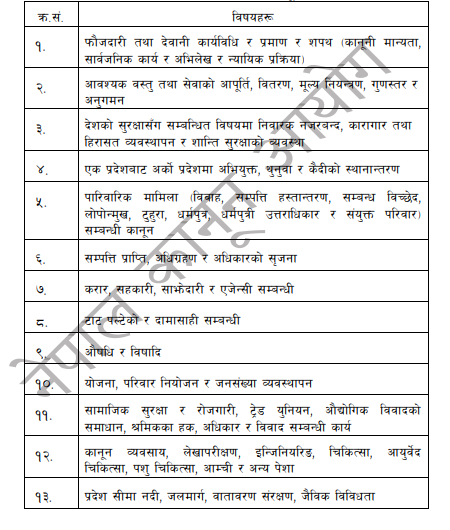
\includegraphics[width=\textwidth]{images/42-1.png}

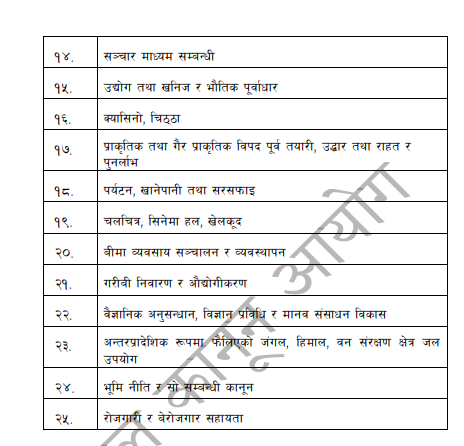
\includegraphics[width=\textwidth]{images/42-2.png}
\pagebreak
\section{अनुसूची–८ स्थानीय तहको अधिकारको सूची}

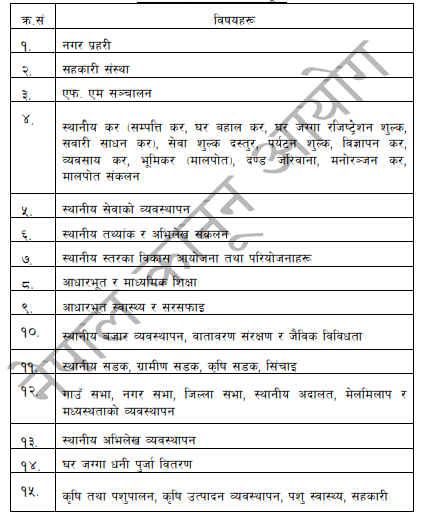
\includegraphics[width=\textwidth]{images/43-1.png}

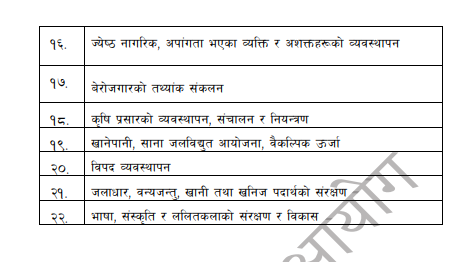
\includegraphics[width=\textwidth]{images/43-2.png}
\pagebreak
\section{अनुसूची–९ संघ, प्रदेश र स्थानीय तहको अधिकारको साझा सूची}

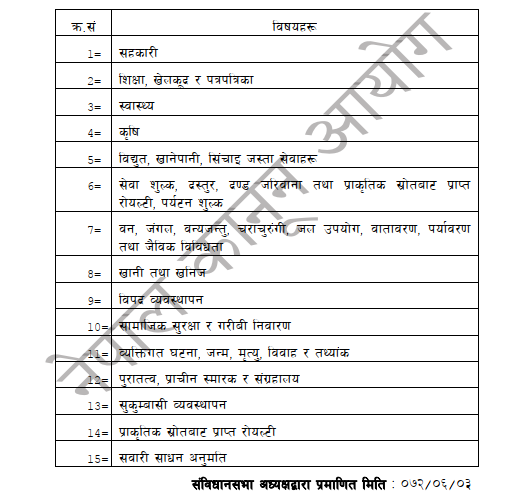
\includegraphics[width=\textwidth]{images/44-1.png}
\pagebreak
\end{document}
